%%%%%%%%%%%%%%%%%%%%%%%%%%%%%%%%%%%%%%%%%%%%%%%%%%%%%%%%%%%%%%%%%%%%%%%%%%%%%%%%%%%%%%%%%
%	Settings of the document
%%%%%%%%%%%%%%%%%%%%%%%%%%%%%%%%%%%%%%%%%%%%%%%%%%%%%%%%%%%%%%%%%%%%%%%%%%%%%%%%%%%%%%%%%


\documentclass[a4paper,12pt,twoside,openright]{book}

% Import all document settings
%----------------------------------------------------------------------------------------
%	Language and font encodings
%----------------------------------------------------------------------------------------


\usepackage[utf8x]{inputenc}
\usepackage[T1]{fontenc}
\usepackage[round]{natbib}
\usepackage[french]{babel}
% french: remove space character after comas in equations
% \DecimalMathComma               


%----------------------------------------------------------------------------------------
%	Sets page size and margins
%----------------------------------------------------------------------------------------


\usepackage{geometry}

%% Pour PDF
\geometry{
	paper=a4paper, % Change to letterpaper for US letter
	% 2,5 cm et 3 cm => textwidth = 21 - 5,5 = 15,5 cm
	inner=2.5cm, % Inner margin
	outer=2.5cm, % Outer margin
	bindingoffset=.5cm, % Binding offset
	top=1.5cm, % Top margin
	bottom=2cm, % Bottom margin
	%showframe, % Uncomment to show how the type block is set on the page
	headheight=4ex,
	includehead,
	includefoot
}

%% Pour impression : avec 2 mm de "fond perdu" à gauche et à droite (version pour rapporteurs avec découpe manuelle)
%\geometry{
%	papersize={21.4cm,29.7cm},
%	% 2,5 cm et 3 cm => textwidth = 21 - 5,5 = 15,5 cm
%	inner=2.7cm, % Inner margin
%	outer=2.7cm, % Outer margin
%	bindingoffset=.5cm, % Binding offset
%	top=1.5cm, % Top margin
%	bottom=2cm, % Bottom margin
%	%showframe, % Uncomment to show how the type block is set on the page
%	headheight=4ex,
%	includehead,
%	includefoot
%}

%% Pour impression : avec 5 mm de "fond perdu" sur chaque côté (version pour repro)
%\geometry{
% 	papersize={22.0cm,30.7cm},
% 	% 2,5 cm et 3 cm => textwidth = 21 - 5,5 = 15,5 cm
% 	inner=3.0cm, % Inner margin
% 	outer=3.0cm, % Outer margin
% 	bindingoffset=.5cm, % Binding offset
% 	top=2.0cm, % Top margin
% 	bottom=2.5cm, % Bottom margin
% 	%showframe, % Uncomment to show how the type block is set on the page
% 	headheight=4ex,
% 	includehead,
% 	includefoot
%}

\setlength{\parindent}{15pt}


%----------------------------------------------------------------------------------------
%	Useful packages
%----------------------------------------------------------------------------------------


\usepackage{calc}
\usepackage{ulem}  % to underline text
\usepackage{pdfpages}  % to integrate pdf pages in the document
\usepackage{hyphenat}  % to specify when hyphenating ('\hyph{}')
\usepackage[autostyle=true]{csquotes}
\usepackage{rotating}


%----------------------------------------------------------------------------------------
%	Maths and symbols
%----------------------------------------------------------------------------------------


\usepackage{icomma}
\usepackage{amsmath}
\usepackage{amssymb}
\usepackage{stmaryrd}  % for double brackets (\llbracket, \rrbracket...)
\setcounter{MaxMatrixCols}{20}
\usepackage{upgreek}  % to display greek letters not in italic in math expressions
\usepackage{marvosym}  % to get the euro symbols
\usepackage{tikz}  % To draw arrows on the side of matrices
\newcommand{\tikzmark}[1]{\tikz[overlay, remember picture] \coordinate (#1);}


%----------------------------------------------------------------------------------------
%	Figures
%----------------------------------------------------------------------------------------


\usepackage{graphicx}
\usepackage[format=plain,labelfont={bf},labelsep=endash]{caption}
\usepackage{subcaption}
% Width of all figure (not subfigures)
\newcommand{\figwidth}{\textwidth}
\usepackage[pagebackref]{hyperref}


%----------------------------------------------------------------------------------------
%	Tables
%----------------------------------------------------------------------------------------


\usepackage{multirow}  % for tables
\renewcommand{\arraystretch}{1.2}


%----------------------------------------------------------------------------------------
%	Mini toc
%----------------------------------------------------------------------------------------


\usepackage[nottoc]{tocbibind}
\usepackage{minitoc}
\setcounter{minitocdepth}{3}

% Space after minitoc
\newlength{\spaceafterminitoc}
\setlength{\spaceafterminitoc}{0.7cm}

% Change the title of minitoc
\addto{\captionsfrench}{% Making babel aware of special titles
  \renewcommand{\mtctitle}{Sommaire}
}


%----------------------------------------------------------------------------------------
%	Acronym settings
%----------------------------------------------------------------------------------------


\usepackage[acronym,toc,shortcuts]{glossaries}
\renewcommand*{\glstextformat}[1]{\textcolor{black}{#1}} % to set the link color of acronyms in text
\makeglossaries
%----------------------------------------------------------------------------------------
%	List of acronym definitions
%----------------------------------------------------------------------------------------


\newacronym{FIRST}{FIRST}{Fibered Interferometer foR a Single Telescope}
\newacronym{FIRSTv1}{FIRSTv1}{Fibered Interferometer foR a Single Telescope version 1}
\newacronym{FIRSTv2}{FIRSTv2}{Fibered Interferometer foR a Single Telescope version 2}
\newacronym{LESIA}{LESIA}{Laboratoire d'\'Etudes Spatiales et d'Instrumentation en Astrophysique}
\newacronym{SCExAO}{SCExAO}{Subaru Coronagraphic Extreme Adaptive Optics}
\newacronym{V2PM}{V2PM}{Visibility To Pixel Matrix}
\newacronym{P2VM}{P2VM}{Pixel To Visibility Matrix}
\newacronym{SVD}{SVD}{Singular Value Decomposition}
\newacronym{CMOS}{CMOS}{Complementary Metal Oxide Semiconductor}
\newacronym{ADU}{ADU}{Analog-Digital Unit}
\newacronym{OPD}{OPD}{Optical Path Difference}
\newacronym{ODL}{ODL}{Optical Delay Line}
\newacronym{MEMS}{MEMS}{Micro-ElectroMechanical Systems}
\newacronym{PSF}{PSF}{Point Spread Function}
\newacronym{UV}{UV}{UltraViolet}
\newacronym{CA}{CA}{Core Accretion}
\newacronym{GI}{GI}{Gravitational Instabilities}
\newacronym{TTS}{TTS}{T Tauri Star}
\newacronym{CTTS}{CTTS}{Classical T Tauri Star}
\newacronym{WTTS}{WTTS}{Weak T Tauri Star}
\newacronym{MUSE}{MUSE}{Multi Unit Spectroscopic Explorer}
\newacronym{VLT}{VLT}{Very Large Telescope}
\newacronym{ELT}{ELT}{Extremely Large Telescope}
\newacronym{NIRC2}{NIRC2}{Near InfraRed Camera 2}
\newacronym{MagAO}{MagAO}{Magellan Adaptive Optics}
\newacronym{LMIRCam}{LMIRCam}{Large binocular telescope Mid-InfraRed Camera}
\newacronym{LBTI}{LBTI}{Large Binocular Telescope Interferometer}
\newacronym{ISIS}{ISIS}{Intermediate-dispersion Spectrograph and Imaging System}
\newacronym{WHT}{WHT}{William Herschel Telescope}
\newacronym{CHARIS}{CHARIS}{Coronagraphic High Angular Resolution Imaging Spectrograph}
\newacronym{SPHERE}{SPHERE}{Spectro-Polarimetic High contrast imager for Exoplanets REsearch}
\newacronym{NACO}{NACO}{Nasmyth Adaptive Optics System - Coude Near Infrared Camera}
\newacronym{GPI}{GPI}{Gemini Planet Imager}
\newacronym{GST}{GST}{Gemini South Telescope}
\newacronym{GAPlanetS}{GAPlanetS}{Giant Accreting Protoplanet Survey}
\newacronym{AMBER}{AMBER}{Astronomical Multi-BEam combineR}
\newacronym{GRAVITY}{GRAVITY}{General Relativity Analysis via VLT InTerferometrY}
\newacronym{SNR}{SNR}{Signal-to-Noise Ratio}
\newacronym{BCD}{BCD}{Beam Commutation Device}
\newacronym{JWST}{JWST}{James Webb Space Telescope}
\newacronym{MIRI}{MIRI}{Mid-Infrared Instrument}
\newacronym{MFD}{MFD}{Mode Field Diameter}
\newacronym{VPH}{VPH}{Volume Phase Holographic}
\newacronym{pyMILK}{pyMILK}{PYthon Multi-purpose Imaging Libraries toolKit}
\newacronym{MILK}{MILK}{Multi-purpose Imaging Libraries toolKit}
\newacronym{SDK}{SDK}{Software Development Kit}
\newacronym{SHM}{SHM}{SHared Memory}
\newacronym{IPAG}{IPAG}{Institut de Plan\'etologie et d'Astrophysique de Grenoble}
\newacronym{RAM}{RAM}{Random Access Memory}
\newacronym{CCD}{CCD}{Charge Coupled Device}
\newacronym{GLINT}{GLINT}{Guided-Light Interferometric Nulling Technology}
% \newacronym{}{}{}

% \newcommand{\aclegend}[1]{(\acs{#1} - \textit{\acl{#1}})}

% https://www.overleaf.com/learn/latex/Glossaries#Compiling_the_glossary
% If you are compiling the document (called main.tex) using pdflatex on your local machine, you have to use these commands:
% pdflatex main.tex
% makeglossaries main
% pdflatex main.tex


%----------------------------------------------------------------------------------------
%	Figure, table and equation numbering
%----------------------------------------------------------------------------------------


\renewcommand{\thefigure}{\thechapter.\arabic{figure}}
\renewcommand{\thetable}{\thechapter.\arabic{table}}
\renewcommand{\theequation}{\thechapter.\arabic{equation}}


%----------------------------------------------------------------------------------------
%	Create a third level of subsection
%----------------------------------------------------------------------------------------


\usepackage{titlesec}
\setcounter{secnumdepth}{4}
\titleformat{\paragraph}{\normalfont\normalsize\bfseries}{\theparagraph}{1em}{}
\titlespacing*{\paragraph}{0pt}{3.25ex plus 1ex minus .2ex}{1.5ex plus .2ex}
\newcommand{\threesubsection}{\paragraph}
\newcommand{\mysubparagraph}[1]{\subparagraph{#1}\mbox{}\\ \mbox{}}


%----------------------------------------------------------------------------------------
%	Abbreviations
%----------------------------------------------------------------------------------------


\newcommand{\vv}[1]{\overrightarrow{#1}}
\newcommand{\ha}[0]{\text{$\text{H}\upalpha$}}
\newcommand{\Lha}[0]{\text{$\text{L}_{\ha}$}}
\newcommand{\Lacc}[0]{\text{$\text{L}_{\text{acc}}$}}
\newcommand{\Wd}[0]{\text{$\text{W}_{10}$}}
\newcommand{\sk}[0]{\textit{Super K}}
\newcommand{\wiggles}[0]{\textit{wiggles}}
\newcommand{\degree}[0]{^{\circ}}
\newcommand{\um}{$\upmu$m}
\newcommand{\Like}[0]{\mathcal{L}}
\newcommand{\MJ}[0]{\text{$\text{M}_\text{J}$}}
\newcommand{\MS}[0]{\text{$\text{M}_{\odot}$}}


%----------------------------------------------------------------------------------------
%	Colored comments
%----------------------------------------------------------------------------------------


\usepackage{xcolor}
\newcommand{\comments}[1]{\textcolor{orange}{#1}}
\newcommand{\kevinco}[1]{\textcolor{red}{#1}}
\newcommand{\elsaco}[1]{\textcolor{blue}{#1}}
\newcommand{\sylvestreco}[1]{\textcolor{green}{#1}}
\usepackage{comment} % to comment parts of the text with \begin{comment} \end{comment}


%----------------------------------------------------------------------------------------
%	
%----------------------------------------------------------------------------------------




%%%%%%%%%%%%%%%%%%%%%%%%%%%%%%%%%%%%%%%%%%%%%%%%%%%%%%%%%%%%%%%%%%%%%%%%%%%%%%%%%%%%%%%%%
%	Begining of the document
%%%%%%%%%%%%%%%%%%%%%%%%%%%%%%%%%%%%%%%%%%%%%%%%%%%%%%%%%%%%%%%%%%%%%%%%%%%%%%%%%%%%%%%%%


\begin{document}

%% A&A bib macros
%
%  These Macros are taken from the AAS TeX macro package version 5.2
%  and are compatible with the macros in the A&A document class
%  version 7.0
%  Include this file in your LaTeX source only if you are not using
%  the AAS TeX macro package or the A&A document class and need to
%  resolve the macro definitions in the TeX/BibTeX entries returned by
%  the ADS abstract service.
%
%  If you plan not to use this file to resolve the journal macros
%  rather than the whole AAS TeX macro package, you should save the
%  file as ``aas_macros.sty'' and then include it in your LaTeX paper
%  by using a construct such as:
%	\documentstyle[11pt,aas_macros]{article}
%
%  For more information on the AASTeX and A&A packages, please see:
%       http://journals.aas.org/authors/aastex.html	
%       ftp://ftp.edpsciences.org/pub/aa/readme.html
%  For more information about ADS abstract server, please see:
%       http://adsabs.harvard.edu/ads_abstracts.html
%

% Abbreviations for journals.  The object here is to provide authors
% with convenient shorthands for the most "popular" (often-cited)
% journals; the author can use these markup tags without being concerned
% about the exact form of the journal abbreviation, or its formatting.
% It is up to the keeper of the macros to make sure the macros expand
% to the proper text.  If macro package writers agree to all use the
% same TeX command name, authors only have to remember one thing, and
% the style file will take care of editorial prefaerences.  This also
% applies when a single journal decides to revamp its abbreviating
% scheme, as happened with the ApJ (Abt 1991).


\newcommand*\aap{A\&A}
\let\astap=\aap
\newcommand*\aapr{A\&A~Rev.}
\newcommand*\aaps{A\&AS}
\newcommand*\actaa{Acta Astron.}
\newcommand*\aj{AJ}
\newcommand*\ao{Appl.~Opt.}
\let\applopt\ao
\newcommand*\apj{ApJ}
\newcommand*\apjl{ApJ}
\let\apjlett\apjl
\newcommand*\apjs{ApJS}
\let\apjsupp\apjs
\newcommand*\aplett{Astrophys.~Lett.}
\newcommand*\apspr{Astrophys.~Space~Phys.~Res.}
\newcommand*\apss{Ap\&SS}
\newcommand*\araa{ARA\&A}
\newcommand*\azh{AZh}
\newcommand*\baas{BAAS}
\newcommand*\bac{Bull. astr. Inst. Czechosl.}
\newcommand*\bain{Bull.~Astron.~Inst.~Netherlands}
\newcommand*\caa{Chinese Astron. Astrophys.}
\newcommand*\cjaa{Chinese J. Astron. Astrophys.}
\newcommand*\fcp{Fund.~Cosmic~Phys.}
\newcommand*\gca{Geochim.~Cosmochim.~Acta}
\newcommand*\grl{Geophys.~Res.~Lett.}
\newcommand*\iaucirc{IAU~Circ.}
\newcommand*\icarus{Icarus}
\newcommand*\jcap{J. Cosmology Astropart. Phys.}
\newcommand*\jcp{J.~Chem.~Phys.}
\newcommand*\jgr{J.~Geophys.~Res.}
\newcommand*\jqsrt{J.~Quant.~Spectr.~Rad.~Transf.}
\newcommand*\jrasc{JRASC}
\newcommand*\memras{MmRAS}
\newcommand*\memsai{Mem.~Soc.~Astron.~Italiana}
\newcommand*\mnras{MNRAS}
\newcommand*\na{New A}
\newcommand*\nar{New A Rev.}
\newcommand*\nat{Nature}
\newcommand*\nphysa{Nucl.~Phys.~A}
\newcommand*\pasa{PASA}
\newcommand*\pasj{PASJ}
\newcommand*\pasp{PASP}
\newcommand*\physrep{Phys.~Rep.}
\newcommand*\physscr{Phys.~Scr}
\newcommand*\planss{Planet.~Space~Sci.}
\newcommand*\pra{Phys.~Rev.~A}
\newcommand*\prb{Phys.~Rev.~B}
\newcommand*\prc{Phys.~Rev.~C}
\newcommand*\prd{Phys.~Rev.~D}
\newcommand*\pre{Phys.~Rev.~E}
\newcommand*\prl{Phys.~Rev.~Lett.}
\newcommand*\procspie{Proc.~SPIE}
\newcommand*\qjras{QJRAS}
\newcommand*\rmxaa{Rev. Mexicana Astron. Astrofis.}
\newcommand*\skytel{S\&T}
\newcommand*\solphys{Sol.~Phys.}
\newcommand*\sovast{Soviet~Ast.}
\newcommand*\ssr{Space~Sci.~Rev.}
\newcommand*\zap{ZAp}


% \let\jnl@style=\rm
% \def\refa@jnl#1{{\jnl@style#1}}

% \def\aj{\refa@jnl{AJ}}                   % Astronomical Journal
% \def\actaa{\refa@jnl{Acta Astron.}}      % Acta Astronomica
% \def\araa{\refa@jnl{ARA\&A}}             % Annual Review of Astron and Astrophys
% \def\apj{\refa@jnl{ApJ}}                 % Astrophysical Journal
% \def\apjl{\refa@jnl{ApJ}}                % Astrophysical Journal, Letters
% \def\apjs{\refa@jnl{ApJS}}               % Astrophysical Journal, Supplement
% \def\ao{\refa@jnl{Appl.~Opt.}}           % Applied Optics
% \def\apss{\refa@jnl{Ap\&SS}}             % Astrophysics and Space Science
% \def\aap{\refa@jnl{A\&A}}                % Astronomy and Astrophysics
% \def\aapr{\refa@jnl{A\&A~Rev.}}          % Astronomy and Astrophysics Reviews
% \def\aaps{\refa@jnl{A\&AS}}              % Astronomy and Astrophysics, Supplement
% \def\azh{\refa@jnl{AZh}}                 % Astronomicheskii Zhurnal
% \def\baas{\refa@jnl{BAAS}}               % Bulletin of the AAS
% \def\bac{\refa@jnl{Bull. astr. Inst. Czechosl.}}
%                 % Bulletin of the Astronomical Institutes of Czechoslovakia 
% \def\caa{\refa@jnl{Chinese Astron. Astrophys.}}
%                 % Chinese Astronomy and Astrophysics
% \def\cjaa{\refa@jnl{Chinese J. Astron. Astrophys.}}
%                 % Chinese Journal of Astronomy and Astrophysics
% \def\icarus{\refa@jnl{Icarus}}           % Icarus
% \def\jcap{\refa@jnl{J. Cosmology Astropart. Phys.}}
%                 % Journal of Cosmology and Astroparticle Physics
% \def\jrasc{\refa@jnl{JRASC}}             % Journal of the RAS of Canada
% \def\memras{\refa@jnl{MmRAS}}            % Memoirs of the RAS
% \def\mnras{\refa@jnl{MNRAS}}             % Monthly Notices of the RAS
% \def\na{\refa@jnl{New A}}                % New Astronomy
% \def\nar{\refa@jnl{New A Rev.}}          % New Astronomy Review
% \def\pra{\refa@jnl{Phys.~Rev.~A}}        % Physical Review A: General Physics
% \def\prb{\refa@jnl{Phys.~Rev.~B}}        % Physical Review B: Solid State
% \def\prc{\refa@jnl{Phys.~Rev.~C}}        % Physical Review C
% \def\prd{\refa@jnl{Phys.~Rev.~D}}        % Physical Review D
% \def\pre{\refa@jnl{Phys.~Rev.~E}}        % Physical Review E
% \def\prl{\refa@jnl{Phys.~Rev.~Lett.}}    % Physical Review Letters
% \def\pasa{\refa@jnl{PASA}}               % Publications of the Astron. Soc. of Australia
% \def\pasp{\refa@jnl{PASP}}               % Publications of the ASP
% \def\pasj{\refa@jnl{PASJ}}               % Publications of the ASJ
% \def\rmxaa{\refa@jnl{Rev. Mexicana Astron. Astrofis.}}%
%                 % Revista Mexicana de Astronomia y Astrofisica
% \def\qjras{\refa@jnl{QJRAS}}             % Quarterly Journal of the RAS
% \def\skytel{\refa@jnl{S\&T}}             % Sky and Telescope
% \def\solphys{\refa@jnl{Sol.~Phys.}}      % Solar Physics
% \def\sovast{\refa@jnl{Soviet~Ast.}}      % Soviet Astronomy
% \def\ssr{\refa@jnl{Space~Sci.~Rev.}}     % Space Science Reviews
% \def\zap{\refa@jnl{ZAp}}                 % Zeitschrift fuer Astrophysik
% \def\nat{\refa@jnl{Nature}}              % Nature
% \def\iaucirc{\refa@jnl{IAU~Circ.}}       % IAU Cirulars
% \def\aplett{\refa@jnl{Astrophys.~Lett.}} % Astrophysics Letters
% \def\apspr{\refa@jnl{Astrophys.~Space~Phys.~Res.}}
%                 % Astrophysics Space Physics Research
% \def\bain{\refa@jnl{Bull.~Astron.~Inst.~Netherlands}} 
%                 % Bulletin Astronomical Institute of the Netherlands
% \def\fcp{\refa@jnl{Fund.~Cosmic~Phys.}}  % Fundamental Cosmic Physics
% \def\gca{\refa@jnl{Geochim.~Cosmochim.~Acta}}   % Geochimica Cosmochimica Acta
% \def\grl{\refa@jnl{Geophys.~Res.~Lett.}} % Geophysics Research Letters
% \def\jcp{\refa@jnl{J.~Chem.~Phys.}}      % Journal of Chemical Physics
% \def\jgr{\refa@jnl{J.~Geophys.~Res.}}    % Journal of Geophysics Research
% \def\jqsrt{\refa@jnl{J.~Quant.~Spec.~Radiat.~Transf.}}
%                 % Journal of Quantitiative Spectroscopy and Radiative Transfer
% \def\memsai{\refa@jnl{Mem.~Soc.~Astron.~Italiana}}
%                 % Mem. Societa Astronomica Italiana
% \def\nphysa{\refa@jnl{Nucl.~Phys.~A}}   % Nuclear Physics A
% \def\physrep{\refa@jnl{Phys.~Rep.}}   % Physics Reports
% \def\physscr{\refa@jnl{Phys.~Scr}}   % Physica Scripta
% \def\planss{\refa@jnl{Planet.~Space~Sci.}}   % Planetary Space Science
% \def\procspie{\refa@jnl{Proc.~SPIE}}   % Proceedings of the SPIE

% \let\astap=\aap
% \let\apjlett=\apjl
% \let\apjsupp=\apjs
% \let\applopt=\ao


%% Build a per-chapter table of content
\dominitoc


%%%%%%%%%%%%%%%%%%%%%%%%%%%%%%%%%%%%%%%%%%%%%%%%%%%%%%%%%%%%%%%%
\pagestyle{empty}
%%%%%%%%%%%%%%%%%%%%%%%%%%%%%%%%%%%%%%%%%%%%%%%%%%%%%%%%%%%
% Karine Perraut <karine.perraut@univ-grenoble-alpes.fr>
% Lucas Labadie <labadie@ph1.uni-koeln.de>
% Arthur Vigan <arthur.vigan@lam.fr>
% Anthony Boccaletti <anthony.boccaletti@obspm.fr>
% Daniel Rouan <daniel.rouan@obspm.fr>
%%%%%%%%%%%%%%%%%%%%%%%%%%%%%%%%%%%%%%%%%%%%%%%%%%%%%%%%%%%

\begin{titlepage}
\parindent=0pt
% www.devoloppez.com \hspace*{\stretch{1}} \LaTeX intermédiaire
% Rubrique \LaTeX\hspace*{\stretch{1}} Tutoriels

% \begin{minipage}{0.33\textwidth}
% \hspace{-1cm}
% \includegraphics[width=\textwidth]{}
% \end{minipage}
% \begin{minipage}{0.33\textwidth}
% \includegraphics[width=\textwidth]{}
% \end{minipage}
% \begin{minipage}{0.33\textwidth}
% \hspace{1cm}
% \includegraphics[width=\textwidth]{}
% \end{minipage}

% \vspace*{\stretch{1}}
% \begin{center}
% % \vspace{-3.4cm}
% \includegraphics[scale=0.2]{}
% \end{center}

\vspace*{\stretch{1}}
\begin{center}\Huge

\end{center}

\hrulefill
\begin{center}\bfseries\Huge
    Caractérisation et intégration de composants d'optique intégrée sur l'interféromètre fibré FIRST au télescope Subaru pour l'étude des protoplanètes en accrétion
\end{center}
% Characterization and deployement of Photonic Integrated Circuits for the FIRST fibered interferometer at the Subaru Telescope in the context of accreting protoplanets studies
\hrulefill

\begin{center}
      du 
\end{center}


\begin{center}\bfseries\Large
par Kevin Barjot
\end{center}

\vspace*{\stretch{1}}
\begin{flushleft}\Large

\end{flushleft}

% \vspace*{\stretch{4}}
% \begin{minipage}{0.2\textwidth}
% \includegraphics[width=0.6\textwidth]{}
% \end{minipage}
% \begin{minipage}{0.4\textwidth}
% \includegraphics[width=1.2\textwidth]{}
% \end{minipage}
% \begin{minipage}{0.4\textwidth}
% \hspace{2cm}
% \includegraphics[width=0.7\textwidth]{}
% \end{minipage}


% \vspace*{\stretch{2}}
% \begin{tikzpicture}[remember picture, overlay]
%  \begin{scope}[shift={(current page.south west)},shift={(1,1)},scale=1]
%  \shade[ball color=blue,opacity=.6] (0,0) circle (10ex);
%  \shade[ball color=blue,opacity=.8] (1.7,1) circle (5ex);
%  \shade[ball color=blue,opacity=.8] (1.5,3) circle (2ex);
%  \shade[ball color=blue,opacity=.5] (-0.5,3) circle (1ex);
%  \shade[ball color=blue,opacity=.8] (1,4) circle (1ex);
%  \shade[ball color=blue,opacity=.6] (3.5,2.5) circle (2ex);
%  \shade[ball color=blue,opacity=.8] (2.5,4.5) circle (4ex);
%  \shade[ball color=blue,opacity=.5] (3,4) circle (3ex);
%  \shade[ball color=blue,opacity=.8] (4.5,4.5) circle (3ex);
%  \shade[ball color=blue,opacity=.5] (5.1,4.7) circle (2ex);
%  \shade[ball color=blue,opacity=.8] (5,6) circle (1.5ex);
%  \shade[ball color=blue,opacity=.6] (3.5,5.5) circle (2ex);
%  \shade[ball color=blue,opacity=.8] (5,3) circle (1ex);
%  \end{scope}
%  \end{tikzpicture}
\end{titlepage}

% Roman page numbering and non-numbered sections still in toc
\frontmatter
\pagestyle{fancy}


%%%%%%%%%%%%%%%%%%%%%%%%%%%%%%%%%%%%%%%%%%%%%%%%%%%%%%%%%%%%%%%%
%----------------------------------------------------------------------------------------
%	FRENCH
%----------------------------------------------------------------------------------------

\newpage
\thispagestyle{empty}
\chapter*{Résumé}

Dans le cadre de ma thèse, j'ai travaillé dans le domaine de l'imagerie haut contraste à haute résolution angulaire (HRA) pour la détection et la caractérisation de compagnon stellaire ou planétaire. Je me suis plus particulièrement intéressé au cas des protoplanètes en cours de formation qui accrètent de la matière, induisant un fort rayonnement à la longueur d'onde \ha. En plus de diminuer le contraste entre l'étoile et la protoplanète à cette longueur d'onde, facilitant sa détection, la mesure de son intensité permettrait d'apporter des contraintes sur ce phénomène à l'oeuvre dans les systèmes planétaires en formation. FIRST (Fibered Interferometer foR a Single Telescope) est un instrument installé sur le banc d'optique adaptative extrême du télescope Subaru (SCExAO) et exploite la technique de masquage et de réarrangement de pupille, qui permet d'atteindre des résolutions angulaires jusqu'à deux fois plus petite que celle du télescope. Pour cela, la pupille d'entrée de l'instrument est sous-divisée en sous-pupilles dont la lumière est injectée dans des fibres optiques monomodes qui appliquent un filtrage spatial du front d'onde supprimant ainsi les aberrations optiques à l'échelle des sous-pupilles. Sur la deuxième version de FIRST (FIRSTv2), la recombinaison de ces faisceaux est effectuée par un composant d'optique intégrée, afin d'augmenter les performances d'imagerie haut contraste. Le développement de la technologie photonique dans le visible est complexe et innovant et l'objectif de ma thèse est d'évaluer ses performances et la faisabilité de son application pour l'imagerie HRA. Cela a nécessité de continuer le développement du banc de test, aussi bien au niveau du montage optique que du logiciel de contrôle, de mettre au point une procédure spécifique d'acquisition des données et de développer un programme de traitement et d'analyse de données.

Une réplique de FIRST a été développée au \ac{LESIA}, afin de pouvoir implémenter, tester et valider les nouveaux développements de composants photoniques avant leur intégration au télescope Subaru. La recombinaison de chaque paire de sous-pupille est ainsi codée sur une ou deux sorties de la puce photonique (selon la technologie utilisée) et sont imagées sur la caméra sur quelques pixels. L'échantillonnage correct des franges d'interférences nécessite une modulation temporelle de la différence de marche. Pour cela, nous utilisons un miroir segmenté contrôlable en position, pour changer le déphasage entre les sous-pupilles. Dans un premier temps, j'ai amélioré le logiciel de contrôle de ce banc pour augmenter sa rapidité ainsi que pour permettre l'acquisition de données interférométriques nécessitant le contrôle synchronisé des différents composants pour la modulation des franges (miroir déformable, lignes à retard et caméra).

J'ai ensuite caractérisé les propriétés optiques de deux puces photoniques qui utilisent deux techniques différentes de recombinaison interférométrique de faisceaux, telles que leur transmission, la quantité de fuite du signal entre les différents guides d'onde (appelé \textit{cross-talk}), leur comportement dans les deux polarisations ainsi que le contraste instrumental. Ensuite, j'ai construit un système optique simulant une source binaire sur le banc de test, qui permet d'injecter à la fois une source avec une large bande spectrale pour simuler une étoile et une source avec une bande spectrale étroite pour simuler une exoplanète avec une raie d'émission. Cela a été crucial pour démontrer les capacités de l'instrument à détecter et mesurer le signal du compagnon. Pour mesurer ce dernier, j'ai tiré profit des propriétés de phase différentielle, qui est une grandeur auto-étalonnée. En effet, la mesure de la phase sur une large bande spectrale permet l'étalonnage des mesures de phases par le signal du continuum mettant en évidence un possible signal dans la raie d'intérêt. J'ai ainsi développé un programme de traitement et d'analyse de données permettant d'estimer la phase différentielle ainsi que la visibilité complexe et la clôture de phase et de les ajuster avec un modèle étoile-compagnon. Cela m'a permis de démontrer que FIRSTv2 pouvait détecter un compagnon de type protoplanète à une séparation équivalente à $0.7 \lambda / B$ de la source centrale, avec un contraste atteignant $0.1$.

Une des puces photoniques a été intégrée dans l'instrument FIRST installé sur le banc SCExAO, ce qui a donné lieu à la première lumière de FIRSTv2 le 10 septembre 2021. J'ai ainsi acquis des données sur ciel lors de plusieurs nuits d'observations à distance mais aussi lors d'une mission à Hawaii en février 2022. Cela a été l'occasion pour moi d'intégrer le deuxième composant pour comparaison avec le premier, ainsi que de déployer le logiciel développé au laboratoire. Les résultats du traitement de ces données sur ciel ont permis d'en apprendre plus sur la méthode d'acquisition et de traitement des données interférométriques.

En conclusion, j'ai caractérisé et étudié les performances de la technologie d'optique intégrée dans le cadre de l'imagerie interférométrique à haut contraste et haute résolution dans le visible. J'ai ainsi développé le logiciel de contrôle de FIRSTv2 en laboratoire avant de le déployer sur le banc SCExAO pour sa première lumière. Ensuite, j'ai développé le programme de traitement et d'analyse de données interférométriques pour FIRSTv2, en y incluant un ajustement des observables interférométriques par un modèle de protoplanète présentant une forte raie d'émission dans son spectre. L'objectif est de caractériser les mécanismes d'accrétion de jeunes systèmes exoplanétaires en formation. Enfin, j'ai eu l'occasion de participer à de nombreuses nuits d'observations durant lesquelles j'ai acquis des données sur des cibles simples telles que des binaires d'étoiles à faible contraste compagnon/étoile.


%----------------------------------------------------------------------------------------
%	ENGLISH
%----------------------------------------------------------------------------------------

\newpage
\thispagestyle{empty}
\chapter*{Abstract}

During my thesis, I worked in the context of high contrast and high angular resolution (HRA) imaging for the detection and the characterisation of stellar or planetary companions. I was particularly interested in the case of forming protoplanets which accrete matter, inducing a strong emission at \ha~wavelength. In addition to decreasing the contrast between the star and the protoplanet at this wavelength, facilitating its detection, the measurement of its intensity would constraints this ongoing phenomenon in protoplanetary systems. FIRST (Fibered Interferometer foR a Single Telescope) is an instrument installed on the Subaru coronagraphic extreme adaptive optics (SCExAO) testbed and exploits the pupil masking and remapping technique, which allows to reach up to twice the angular resolutiono of the telescope. To achieve this, the instrument's entrance pupil is subdivided into sub-pupils whose light is injected into single-mode optical fibres that spatially filter the wavefront, thereby suppressing optical aberrations at the sub-pupil level. In the second version of FIRST (FIRSTv2), the recombination of these beams is performed by an integrated optics component in order to increase the high contrast imaging performance. The development of photonic technology in the visible range is complex and innovative and the objective of my thesis is to evaluate its performance and the feasibility of its application for HRA imaging. In that purpose I conducted the further development of the testbed, both in terms of the optical setup and the control software, developed a specific data acquisition procedure and a data processing and analysis pipeline.

A replica of FIRST has been built at LESIA, in order to implement, test and validate new developments of photonic components before their integration at the Subaru telescope. The recombination of each pair of sub-pupils is encoded on one or two outputs of the photonic chip (depending on the technology used) and imaged on the camera on a few pixels. The correct sampling of the interference fringes requires a temporal modulation of the optical path difference (OPD). For this purpose, we use a segmented mirror controllable in piston and tip/tilt to change the phase shift between the sub-pupils. First, I improved the control software of the testbed to increase its speed and to allow the acquisition of interferometric data requiring the synchronised control of the different components for the modulation of the fringes (deformable mirror, delay lines and camera).

Then I characterised the optical properties of two photonic chips that use two different interferometric beam recombination techniques, such as their transmission, the cross-talk between the waveguides, their behaviour in the two polarisations and the instrumental contrast. I built an optical system simulating a binary source on the testbed, which allows to inject both a source with a wide spectral band to simulate a central star and a source with a narrow spectral band to simulate an exoplanet with an emission line. This was crucial to demonstrate the instrument's ability to detect and measure the companion signal. To measure the latter, I took advantage of the properties of spectral differential phase, which is a self-calibrated quantity. Indeed, the measurement of the phase over a wide spectral band allows the calibration of the phase measurements by the continuum signal highlighting a possible signal in the emission line of interest. Thus, I developed a data processing and analysis program allowing to estimate the differential phase as well as the complex visibility and the closure phase and to fit them with a star-companion model. Therefore I was able to demonstrate that FIRSTv2 could detect a protoplanet-like companion at an equivalent separation of $0.7 \lambda / B$ from the central source, with a contrast of up to $0.1$.

One of the photonic chips was integrated to the FIRST instrument installed on the SCExAO bench, resulting in the first light from FIRSTv2 on 10 September 2021. I acquired on-sky data during several remote observation nights as well as during a mission to Hawaii in February 2022. It was the opportunity for me to integrate the second component for comparison with the first, as well as to deploy the control software developed in the laboratory. The results of the processing of these on-sky data allowed me to learn more about the acquisition and processing methods of interferometric data.

To conclude, I characterised and studied the performance of the integrated optics technology in the context of high contrast and high resolution interferometric imaging in the visible range. I developed the FIRSTv2 control software in the laboratory before deploying it on the SCExAO bench for the first light. Then, I developed the interferometric data processing and analysis program for FIRSTv2, including a fitting of the interferometric observables by a protoplanet model with a strong emission line in its spectrum. The objective is to characterise the accretion mechanisms of young exoplanetary systems in formation. Finally, I have had the opportunity to participate in many observing nights during which I have acquired data on simple targets such as companion-star binaries with low contrast.




%%%%%%%%%%%%%%%%%%%%%%%%%%%%%%%%%%%%%%%%%%%%%%%%%%%%%%%%%%%%%%%%
\newpage
\thispagestyle{empty}
\begingroup
\hypersetup{linkcolor=black}
\tableofcontents
\endgroup

% Re-initialize page numbering and set it to arabic numbers
\mainmatter


%%%%%%%%%%%%%%%%%%%%%%%%%%%%%%%%%%%%%%%%%%%%%%%%%%%%%%%%%%%%%%%%
\clearpage
%%%%%%%%%%%%%%%%%%%%%%%%%%%%%%%%%%%%%%%%%%%%%%%%%%%%%%%%%%%%%%%%
\section{Introduction}
\setcounter{figure}{0}
\setcounter{table}{0}

%%%%%%%%%%%%%%%%%%%%%%%%%%%%%%%%
\subsection{Imagerie haut contraste et haute résolution angulaire pour l'étude des exoplanètes}

%%%%%%%%%%%%%%%%
\subsubsection{L'étude des exoplanètes}
% https://www.britannica.com/biography/Giordano-Bruno

Depuis la première détection d'une exoplanète, 51 Peg b \citep{mayor1995}, en (la bonne année) $1995$, les techniques de détection et de caractérisation de systèmes exoplanétaires n'ont cessées de gagner en sensibilité et de se diversifier. Les détections de plus de $5\,000$ exoplanètes sont confirmées à ce jour et la figure~\ref{fig:ExoplanetDetection} présente une partie de ces détections (celles dont le demi-grand axe a pu être mesuré), pour les quatre techniques de détection par vitesse radiale (cercle orange), par transite (triangle vert), par micro-lentille gravitationnelle (point violet) et par imagerie directe (carré bleu). La masse (en unité de masse de Jupiter) de l'exoplanète est tracée en fonction de son demi-grand axe en \ac{AU} ou \ac{UA}, en français. Les huit planètes du système solaire y sont aussi représentées pour comparaison, par la première lettre de son nom dans une bulle. Enfin, seule les corps ayant une masse inférieure à $13 \,$\MJ (correspondant à la définition d'une planète) ce qui induit un plafonnement horizontal des corps détectés en haut du graphique.

\begin{figure}[ht!]
    \centering
    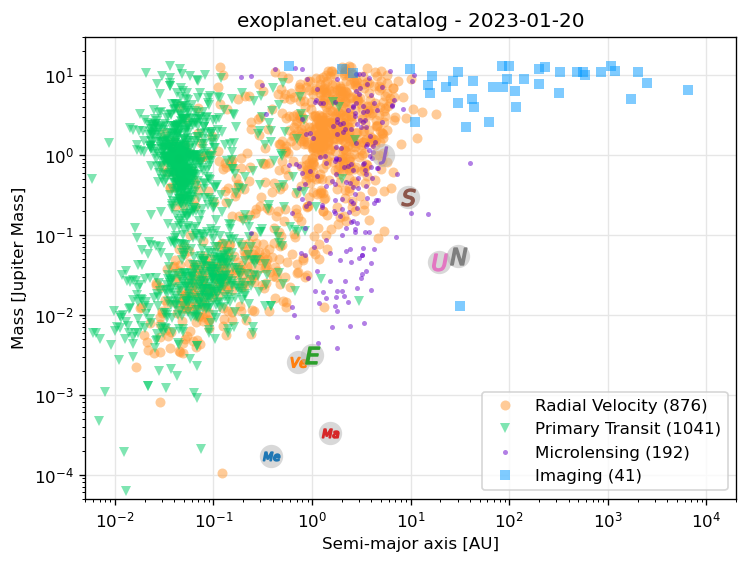
\includegraphics[width=0.8\textwidth]{Figure_Chap1/20230120_exoplanet_diagram_RV_PT_ML_IM.png}
    \caption[Graphique des exoplanètes détectées à ce jour suivant les quatre techniques de détection principales.]{Graphique de la masse mesurées des exoplanètes détectées à ce jour en fonction de leur demi-grand axe estimé. Les détections sont identifiées par les techniques de détection par vitesse radiale (cercle orange), par transite (triangle vert), par micro-lentille gravitationnelle (point violet) et par imagerie directe (carré bleu). Seules $2\,150$ exoplanètes, dont le demi-grand axe est mesuré, sont affichées. Données tirées de la base de données de \textit{exoplanet.eu} (\url{http://exoplanet.eu/}).}
    \label{fig:ExoplanetDetection}
\end{figure}

On remarque que les deux techniques de transite et de vitesse radiale (méthode qui détecte pour la première fois 51 Peg b) ont permis de détecter la majorité des exoplanètes. Cela s'explique par le fait qu'elles sont les plus simples techniquement à implémenter en comparaison des autres. Les missions spatiales Kepler \citep{borucki2010} et \ac{TESS} \citep{ricker2016} ont ainsi été lancées afin de détecter et étudier de nouvelles exoplanètes par la méthode des transites. Ces deux missions ont permis de détecter plus de $2\,700$ et $300$ (pour $6\,000$ candidats) nouvelles exoplanètes, respectivement.

De plus, on remarque que chaque technique de détection découvre une population d'exoplanètes qui sont homologues, se traduisant sur le graphique par un regroupement des points par technique de détection avec peu de chevauchement. En effet, la méthode des transites mesure le passage du compagnon devant son étoile ce qui favorise la détection de ceux qui ont un petit demi-grand axe car cela augmente le nombre de passage et les chances qu'il passe entre l'étoile et la Terre. La méthode des vitesses radiales mesure le déplacement de l'étoile dans la ligne de visée et ce déplacement est d'autant plus élevé que le compagnon est massif ou lorsque le compagnon est plus proche de l'étoile s'il est moins massif. La méthode d'imagerie consistant en l'observation de la lumière provenant du compagnon, elle est plus sensible aux systèmes avec une grande séparation et dont l'exoplanète est très massive (voir plus de détails dans la section~\ref{sec:ImagerieDirecte}) : elle réfléchis alors plus de lumières de son étoile ou émet un rayonnement de plus forte intensité lorsque c'est une exoplanète de type Jupiter chaude nouvellement formée. Enfin, la méthode de micro-lentille gravitationnelle qui consiste à détecter l'augmentation du flux lumineux d'une étoile en arrière-plan par l'effet de lentille gravitationnelle du compagnon d'un système exoplanétaire en avant-plan, est sensible pour une séparation idéale avec l'étoile qui ne peut ni être trop petite car on ne pourrait pas discerner l'effet de lentille de l'étoile de celui du compagnon, ni trop grande car les chances qu'à la fois l'étoile et le compagnon passent devant l'étoile d'arrière-plan sont faibles.

Par conséquent, il est nécessaire de garder à l'esprit que l'exploration de l'espace des paramètres des exoplanètes détectées est limitée et biaisée par la méthode de détection utilisée. Cela motive l'amélioration des technologies existantes et la recherche de nouvelles solutions techniques afin d'accéder à des cas différents d'exoplanètes pour diversifier l'ensemble des connaissances sur les systèmes planétaires. L'imagerie directe a encore peu explorer cet espace des paramètres et se révèle très intéressante en ce qu'elle permet l'étude spectroscopique et photométrique des exoplanètes ce qui est un atout majeur dans la recherche de traces de vie extra-terrestre.


%%%%%%%%%%%%%%%%
\subsubsection{L'imagerie directe des systèmes exoplanétaires}
\label{sec:ImagerieDirecte}

\kevinco{j'ai tiré pas mal des refs de cette partie de currie2022, j'espère que ça ne s'apparente pas à du plagiat ou que c'est ok...}

L'imagerie directe d'un système exoplanétaire permet d'une part l'étude du mouvement orbital du compagnon \citep{chauvin2012, wang2018} et d'autre part la mesure spectroscopique du compagnon. Cette dernière rend possible l'étude de la composition chimique de l'atmosphère de la planète (détection de la présence d'eau ou de molécules organiques comme le méthane ou le monoxyde de carbone), d'inférer la présence de nuages \citep{marley2015} (en ajustant des modèles atmosphériques), la gravité de surface \citep{marley2012} (la présence de nuages dans l'atmosphère et sa chimie sont fortement influencées par la gravité de surface) ou la rotation de l'exoplanète \citep{bryan2020} (à partir de l'élargissement des raies spectrales). Actuellement, seulement une vingtaine d'images directes de systèmes exoplanétaires ont été obtenues \citep{currie2022} car les performances à atteindre sont ambitieuses. En effet, il s'agit de relever deux défis techniques majeures : un grand pouvoir de résolution angulaire et un haut contraste.

Pour illustrer ce propos, la figure~\ref{fig:ContrastSeparation} tirée de \cite{mawet2012} présente le contraste de l'intensité lumineuse entre le compagnon et l'étoile centrale (\textit{Planet/Star Contrast}) en fonction de la séparation apparente, pour les planètes du système solaire (dans la partie inférieur du graphique) telles qu'elles seraient observées à une distance de $10 \,$pc (distance typique entre la Terre et les systèmes exoplanétaires) ainsi que pour les exoplanètes imagées du système HR8799 \citep{marois2008} et $\upbeta$ Pic b \citep{lagrange2010} (dans la partie supérieur du graphique). Les domaines de performances de quelques instruments en services et futurs sont représentés par les lignes colorées nommées par leur nom. On remarque que les performances à atteindre pour observer des planètes telles que celles du système solaire sont encore hors d'atteinte de $1-2$ ordres de grandeur par les instruments futurs (en cours de construction) et de $2-4$ ordres de grandeur pour les instruments actuels.

\begin{figure}[ht!]
    \centering
    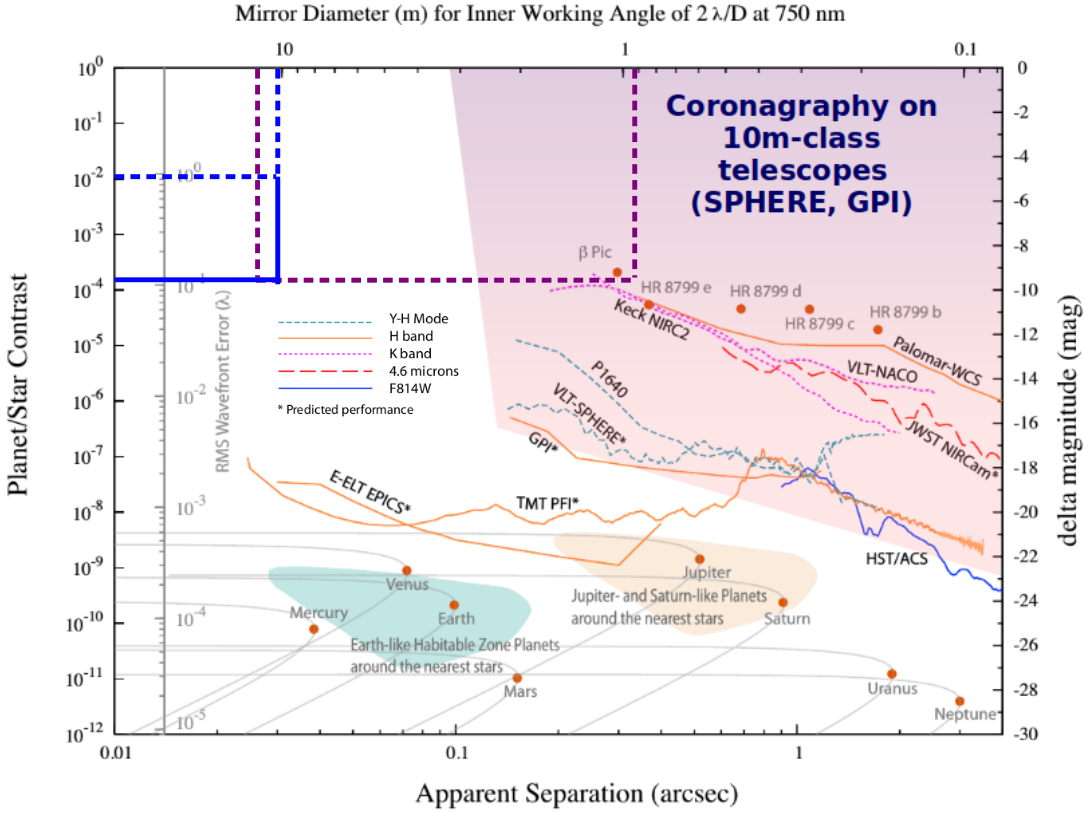
\includegraphics[width=0.8\textwidth]{Figure_Chap1/Mawet2012_ContrastVSSeparation_InstruPerformances_02.png}
    \caption[Contraste en fonction de la séparation apparente de certaines exoplanètes imagées et des planètes du système solaire.]{Contraste (\textit{Planet/Star Contrast}) en fonction de la séparation apparente (en arcsec) des exoplanètes du système HR8799 (bcde) et de $\upbeta$ Pic b (dans la partie supérieur) et des planètes du système solaire telles que vu à une distance de $10 \,$pc (dans la partie inférieur). Un deuxième axe des ordonnées, à gauche, indique l'erreur rms (en unité de longueur d'onde) sur le front d'onde à atteindre pour imager un système exoplanétaire au contraste correspondant à la même ordonnée. Un troisième axe des ordonnées, à droite, indique la différence de magnitude entre l'étoile et la planète. Les limites hautes des performances de quelques instruments actuels (Keck-NIRC2, VLT-NACO, Palomar-WCS, HST-ACS, GPI, SPHERE, Palomar-P3K-P1640 et JWST-NIRCam) et de futurs instruments (TMT-PFI et E-ELT-EPICS) sont tracées par les lignes colorées (on note que ce graphique datant de 2012, il indique par une étoile certains futurs projets qui sont actuellement en fonctionnement). La zone de couleur violette dégradée indique le domaine de performances des systèmes coronographiques sur les télescopes de $10 \,$m. Le rectangle en tirets violets indique le domaine de performances de la technique de masquage de pupille sur les télescopes de $10 \,$m. Les rectangles en tirets bleus et en trait continu bleu indiquent les domaines de performance de la technique de masquage de pupille dans le visible des instruments FIRSTv1 et FIRSTv2, respectivement.}
    \label{fig:ContrastSeparation}
\end{figure}

Le premier défi technique à relever est le haut contraste qui est définis comme le rapport entre l'intensité lumineuse de la planète par celle de l'étoile. Celui-ci atteint $\sim 10^{-3}$ dans le cas des planètes géantes gazeuses qui émettent un rayonnement thermique infrarouge. Ce sont la plupart des systèmes imagés actuellement (car plus facilement détectables) mais sont une population restreinte dans la taxonomie des exoplanètes car ce sont des systèmes très jeunes (de l'ordre de la dizaine de millions d'années ou moins). Mais encore, le contraste est de $\sim 10^{-10}$ pour les planètes de type terrestre. Ce sont des systèmes plus vieux (de l'ordre de centaines de millions à plusieurs milliards d'années) dans lesquels le compagnon réfléchit la lumière de l'étoile dans le visible et constituent donc un plus grand intérêt dans le cadre de la recherche de traces de vie extra-terrestre mais les systèmes imagés jusque maintenant sont majoritairement dans la première catégorie. La technique de la coronographie \citep{lyot1939} a été la plus largement utilisée pour obtenir ces images et son domaine de performance est représenté en dégradé de violet sur la figure~\ref{fig:ContrastSeparation}. Le composant principal de cette technique est un coronographe et il permet de supprimer par interférence destructive la lumière incidente de l'étoile centrée sur son axe optique, tout en laissant apparaître la lumière du compagnon décentré par rapport à l'étoile. En revanche, les perturbations atmosphériques qui perturbent le front d'onde incident lors d'observations au sol diminuent fortement les performances de cette technique. Sur la même figure, un deuxième axe vertical à gauche indique l'erreur rms maximum du front d'onde afin d'obtenir la performance en contraste correspondante. Il s'agit d'erreurs de l'ordre de $100 \,$nm et de $0,01 \,$nm dans les cas des systèmes précédemment imagés dans l'infrarouge et des exoplanètes de type terrestre observées dans le visible, respectivement. Il est donc nécessaire de corriger les perturbations atmosphérique en amont du coronographe \citep{sivaramakrishnan2001} à l'aide de systèmes d'optique adaptative \citep{rousset1990} et d'optique adaptative extrême, qui permettent d'atteindre aujourd'hui des contrastes en entrée de l'instrument de $10^{-3}$ à $10^{-4,5}$ : e.g. \ac{LBTAO} \citep{esposito2011}, PALM-3000 sur le télescope Hale de l'observatoire Palomar \citep{dekany2013}, \ac{GPI} sur le télescope Gemini-South \citep{macintosh2014}, \ac{SPHERE} \citep{beuzit2019} sur le \ac{VLT}, \ac{SCExAO} \citep{jovanovic2015} sur le télescope Subaru, \ac{MagAO-X} \citep{males2020} sur le télescope Clay de l'observatoire Magellan. \kevinco{ajouter peut-être les nouvelles techniques de la correction temps réel des speckles (THD2, ZELDA, SPEED) ?}

Le deuxième défi est d'atteindre un fort pouvoir de résolution angulaire car il s'agit ici de détecter la lumière d'un point se trouvant à de très petites distances apparentes : de l'ordre de $10 - 100 \,$mas, ce qui correspond à $\sim 2-3 \,$AU à une distance de la Terre de $100 - 10 \,$pc. Hors la coronographie n'est performante que pour des grandes séparations angulaires (typiquement à plus de $4 \uplambda / \text{d}$ de l'étoile centrale) car la lumière de l'étoile parvient à fuir aux petites séparations ce qui rend difficile la détection de compagnon trop proches. De nouveaux concepts voient le jour pour améliorer cette performance des coronographes \citep{mawet2012} mais ils parviennent encore difficilement à des séparations de l'ordre de la limite de diffraction $\uplambda / \text{d}$. Le masquage de pupille (voir la section~\ref{sec:PupilMasking}) est une technique permettant d'augmenter le pouvoir de résolution en imagerie jusqu'à $0,5 \uplambda / \text{d}$. Son domaine de performance est tracé sur la figure~\ref{fig:ContrastSeparation} par les rectangles en tirets violets, en tirets bleus et en trait continu bleu sur des télescopes de $8 - 10 \,$m dans l'infrarouge, le visible sur \ac{FIRSTv1} et dans le visible sur \ac{FIRSTv2}, respectivement. On note l'intérêt d'observations dans le visible associées à de meilleurs résolutions angulaires et les bas contrastes jusqu'alors atteint $< 10^{-4}$ par cette technique dû à sa nature peu transmissive.

Enfin, des programmes de traitement et d'analyse de données élaborés permettent d'augmenter un peu plus les performances de contrastes sur les images, de $1 - 2$ ordre de grandeur : e.g. \ac{ADI} \citep{marois2006}, \ac{SDI} \citep{marois2000}, \ac{RDI} \citep{lafreniere2009}. C'est en combinant toutes ces applications instrumentales (optique adaptative, coronographie et traitement de données approfondis) qu'il a été possible d'imager directement quelques systèmes exoplanétaires. Cela a permis d'ouvrir un nouveau domaine de l'étude des exoplanètes qui grandit toujours actuellement et qui a encore beaucoup à faire. Parmi les différentes voies existante, l'interférométrie est une technique proposant d'atteindre de meilleures performances en résolution angulaire de plusieurs ordres de grandeur et c'est dans ce cadre que s'inscrit mon travail de thèse.


%%%%%%%%%%%%%%%%%%%%%%%%%%%%%%%%
\subsection{L'instrument FIRST dans le contexte de l'imagerie directe des exoplanètes}

%%%%%%%%%%%%%%%%
\subsubsection{L'interférométrie}

En reprenant les explications présentées dans la section 1.2.1 de la thèse d'Elsa Huby \citep{huby2013these}, chaque paire de points du front d'onde incident à un télescope interfère et produit un interférogramme dans le plan focal. Ainsi, la tâche de diffraction dans le plan focal du télescope peut s'interpréter comme la superposition de l'ensemble de ces interférogrammes. Pour un front d'onde provenant d'une source lumineuse astrophysique (à l'infini) non résolue incident à un télescope avec une pupille d'entrée circulaire, de diamètre D, la tâche de diffraction au plan focal est une fonction d'Airy, dont l'expression s'écrit :

\begin{equation}
    \text{I}_{\text{Airy}}(x) = \left( \frac{2 \text{J}_{1} (\uppi \text{D}x / \uplambda \text{f})}{\uppi \text{D}x / \uplambda \text{f}} \right)^2
\end{equation}

\noindent où f est la distance focale du télescope et $\text{J}_{1}$ est la fonction de Bessel de première espèce d'ordre 1.

Le pouvoir de résolution du télescope est défini par la largeur à mi-hauteur de cette tâche de diffraction, qui s'écrit : $\uplambda / \text{D}$. Cela correspond au plus petit détail discernable par un télescope. De la même manière, la recombinaison interférométrique des deux faisceaux collectés à la sortie de deux télescopes séparés d'une distance B, appelée base, qui observent simultanément une source lumineuse donne un interférogramme équivalent à celui résultant de l'interférence de deux points séparés d'une distance B sur la pupille d'un télescope. Ainsi, la recombinaison de ces deux faisceaux permet l'observation d'une cible astrophysique avec un pouvoir de résolution égal à $\uplambda / \text{B}$ qui peut être augmenté en éloignant les télescopes, évitant ainsi la construction d'un télescope monolithique de diamètre égal à B.

C'est ce principe qui est implémenter actuellement dans les observatoires \ac{CHARA} \citep{tenbrummelaar2005} sur le Mont Wilson, qui peut combiner six télescopes de $1 \,$m de diamètre, avec des bases de $330 \,$m de longueur, dans l'infrarouge et \ac{VLTI} \citep{haguenauer2012} sur le Cerro Paranal, qui peut combiner quatre télescopes de $\sim 8 \,$m et quatre télescopes de $\sim 2 \,$m de diamètre, avec des bases de $130 \,$m de longueur, dans l'infrarouge proche et moyen. C'est aussi de cette façon que la première image de l'environnement proche du trou noir du centre de la galaxie M87 a été construite \citep{EHTC2019}, à partir de la combinaison des faisceaux radio de télescopes répartis sur Terre, offrant une base de longueur de son diamètre ($\sim 10^4 \,$km). Mais encore, le futur projet \textit{hypertélescope} \citep{labeyrie2013} a pour ambition de combiner les faisceaux de télescopes espacés jusqu'à $10^5 \,$km dans l'espace pour l'étude galactique, l'étude de surface stellaire et l'imagerie directe d'exoplanètes.

Ici, je ne m'intéresse qu'à l'interférométrie optique, qui a ses contraintes techniques spécifiques comparé à l'interférométrie radio ou infrarouge. Premièrement, sans doute la plus exigeante est de s'assurer que les faisceaux collectés par les différents télescopes soit combinés sans retard de phase. Pour cela, les longueurs parcourues par les différents faisceaux sont ajustées grâce à des lignes à retard. Deuxièmement, les technologies de recombinaison des faisceaux proviennent du domaine des télécommunications infrarouges et l'adaptation au visible n'est pas directe (plus de détails dans la section~\ref{sec:PhotonicChip}).


% avantage de la CP qui est une observable auto calibrée
% On the sensitivity of closure phases to faint companions in optical long baseline interferometry https://ui.adsabs.harvard.edu/abs/2012A%26A...541A..89L/abstract
% @ transition à faire
% @ transition à faire
% @ transition à faire
% @ transition à faire
% @ transition à faire
% @ transition à faire
% @ transition à faire
% @ transition à faire
% @ transition à faire
% @ transition à faire
% @ transition à faire
% @ transition à faire
% @ transition à faire
% @ transition à faire


%%%%%%%%%%%%%%%%
\subsubsection{Les techniques de masquage et réarrangement de pupille}
\label{sec:PupilMasking}

Comme nous l'avons vu dans la partie précédente, la figure mesurée dans le plan focal d'un télescope est la superposition d'une infinité d'interférogrammes. Ainsi, une infinité de paires de points de base égale à $\vv{\text{B}}$ (repéré dans le plan pupille) contribuent à une infinité d'interférogrammes de fréquence spatiale égale à $\vv{\text{B}} / \uplambda$ (avec $\uplambda$ la longueur d'onde d'observation) qui se superposent lorsqu'ils sont imagés. Dans le cas où le front d'onde incident est perturbé par la turbulence atmosphérique, y compris après la correction par un système d'optique adaptative qui laisse des résidus, ces paires de points sont déphasés et les interférogrammes (de même fréquence spatiale) ne se superposent plus. Ces perturbations brouillent les franges ce qui induit une diminution du pouvoir de résolution de l'instrument. 

La technique de masquage de pupille \citep{baldwin1986, haniff1987} propose d'appliquer un masque comportant des trous sur la pupille du télescope afin de sélectionner des paires de sous-pupille disposées de façon non-redondante. La non-redondance assure une unique contribution de la part des paires de sous-pupilles à chaque interférogramme ce qui empêche le brouillage des franges. Cela a, par exemple, été implémenté sur l'un des télescopes Keck \citep{tuthill2000}. La figure~\ref{fig:KeckPupilMaskingA} présente le masque utilisé, disposant de $21$ trous, superposé au miroir primaire. La figure~\ref{fig:KeckPupilMaskingB} est une image du détecteur obtenue lors d'une observation avec le masque installé. La tâche est la superposition de $21 \times 20 / 2 = 210$ réseaux de franges. Enfin, la figure~\ref{fig:KeckPupilMaskingC} est la transformée de Fourier de l'image précédente, que l'on nomme plan UV des fréquences spatiales. On remarque que ce plan est échantillonné et donne l'information sur $210$ fréquences spatiales indépendantes.

\begin{figure}[ht!]
    \centering
    \begin{subfigure}[t]{0.3\textwidth}
        \centering
        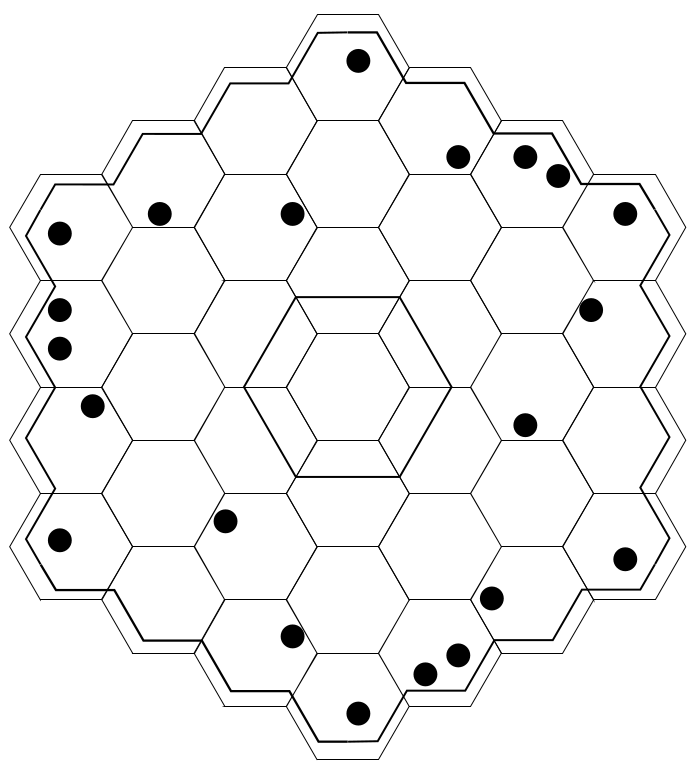
\includegraphics[width=0.9\textwidth]{Figure_Chap1/Tuthill2000_Figure3a.png}
        \caption{Pupille du télescope avec le masque. Le miroir du télescope est composé d'un pavage de segments hexagonaux et les trous du masque sont représentés par des points noirs.}
        \label{fig:KeckPupilMaskingA}
    \end{subfigure}
    \begin{subfigure}[t]{0.3\textwidth}
        \centering
        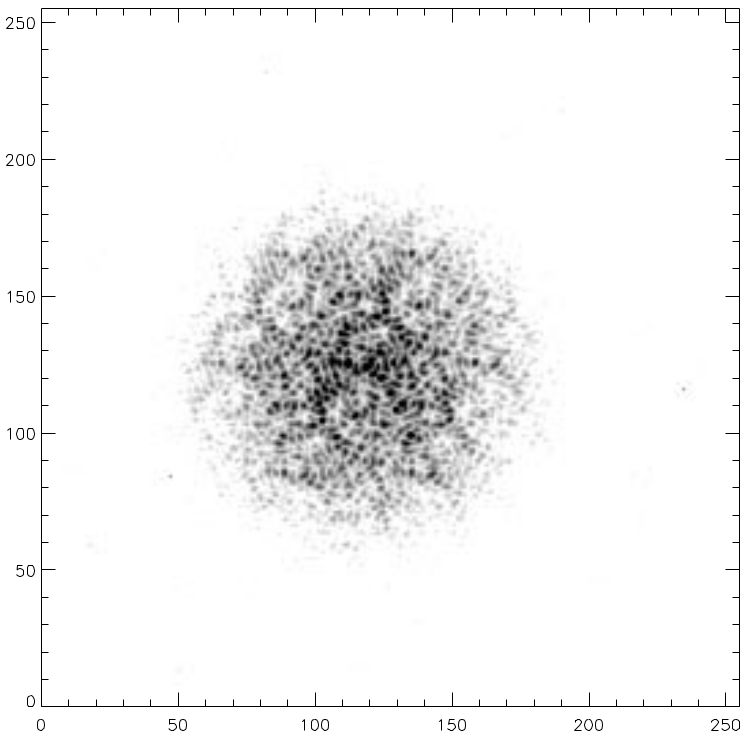
\includegraphics[width=0.9\textwidth]{Figure_Chap1/Tuthill2000_Figure3b.png}
        \caption{Image des réseaux de franges obtenus sur la caméra.}
        \label{fig:KeckPupilMaskingB}
    \end{subfigure}
    \begin{subfigure}[t]{0.3\textwidth}
        \centering
        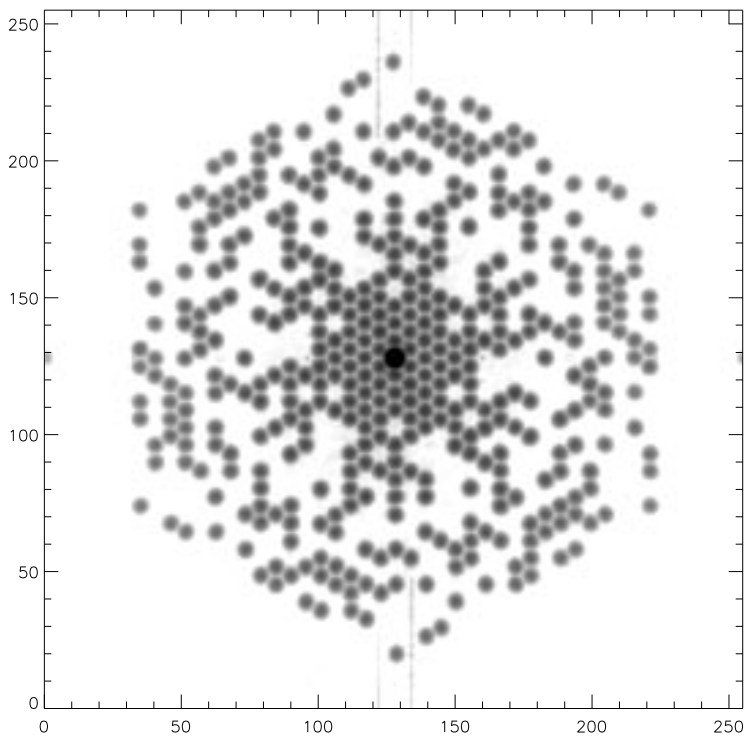
\includegraphics[width=0.9\textwidth]{Figure_Chap1/Tuthill2000_Figure3c.png}
        \caption{Plan UV obtenu par la transformé de Fourier de l'image de la caméra.}
        \label{fig:KeckPupilMaskingC}
    \end{subfigure}
    \caption[Expérience de masquage de pupille sur l'un des télescope Keck.]{Expérience de masquage de pupille sur l'un des télescope Keck. Figures tirées de \cite{tuthill2000}.}
    \label{fig:KeckPupilMasking}
\end{figure}

Cette technique est utilisée comme mode d'observation \ac{SAM} sur l'instrument \ac{NACO} \citep{tuthill2010, lacour2011a} du \ac{VLT}, sur l'instrument \ac{SPHERE} \citep{cheetham2016} du même télescope, ainsi que sur l'instrument \ac{NIRISS} du télescope spatiale \ac{JWST} \citep{sivaramakrishnan2012}. Ce mode est aussi prévu pour l'instrument \ac{MICADO} \citep{lacour2014} du futur télescope \ac{E-ELT} de $39 \,$m de diamètre.

L'avantage majeur de cette technique est qu'il est possible d'atteindre, après analyse des données, un pouvoir de résolution allant jusqu'à $0,5 \uplambda / \text{D}$ où D étant le diamètre du télescope \citep{lacour2011b}. En revanche son désavantage majeur est sa faible transmission du flux lumineux à cause de la faible exploitation de la pupille d'entrée du télescope. E.g. le masque de la figure~\ref{fig:KeckPupilMaskingA} a une transmission du flux lumineux de $10\%$.

Afin de contrebalancer ce problème, le réarrangement de pupille est proposé \citep{perrin2006, lacour2007}. Elle permet  d'exploiter l'entièreté de la pupille du télescope en combinaison avec la technique de masquage de pupille. Pour cela, toute la pupille est divisée en sous-pupille afin d'être réarrangées de manière non-redondante. Pour ce faire, le flux lumineux des faisceaux de chaque sous-pupille est injecté dans des fibres optiques mono-modes. Celles-ci permettent à la fois le réarrangement simple des sous-pupilles et le filtrage du front d'onde de chaque sous-pille des résidus de phase subsistant après l'optique adaptative. \ac{FIRST} est le premier instrument implémentant cette technique de réarrangement de pupille fibré \citep{kotani2008} pour l'imagerie haut contraste à haute résolution angulaire.

Enfin, l'instrument \ac{GLINT} \citep{martinod2021} propose une autre solution technique du réarrangement de pupille, sans fibres optiques, en injectant directement les faisceaux dans un composant d'optique intégré (servant à la recombinaison interférométrique). Les entrées ont alors la même disposition spatiale que celle des sous-pupilles. Les faisceaux sont ensuite guidés dans le composant avant d'être recombinés par paire.

Comme on vient de le voir, ces techniques atteignent un pouvoir de résolution allant jusqu'à $0,5 \uplambda / \text{D}$. Le masquage de pupille sur un télescope unique de $8 \,$m de diamètre permet des mesures sur un compagnon d'étoile avec une séparation de l'ordre de la dizaine de mas. De plus, l'étude faite par \cite{fernandes2019} sur la population des planètes géantes ($0,1 - 20 \text{M}_{\text{J}}$) détectées par la méthode des vitesses radiales et par la mission Kepler, résumée par le graphique de la figure~\ref{fig:Fernandes2019F2}, montre une forte occurrence des exoplanètes avec un demi-grand axe égale à $\sim 2 \,$AU. Or pour des systèmes exoplanétaires à une distance d'environ $100 \,$pc de la Terre (la distance où se trouvent la plupart des nébuleuses d'étoiles en formation) avec de telles valeurs de demi-grand axe, présentent une séparation projetée sur le ciel qui vaut $\sim 10 \,$mas. On voit donc ici l'intérêt du développement d'instrument implémentant la technique de masquage de pupille sur les télescopes de la classe $10 \,$m de diamètre : cela ouvre le champ de l'imagerie directe à une toute nouvelle population d'exoplanètes. 

\begin{figure}[ht!]
    \centering
    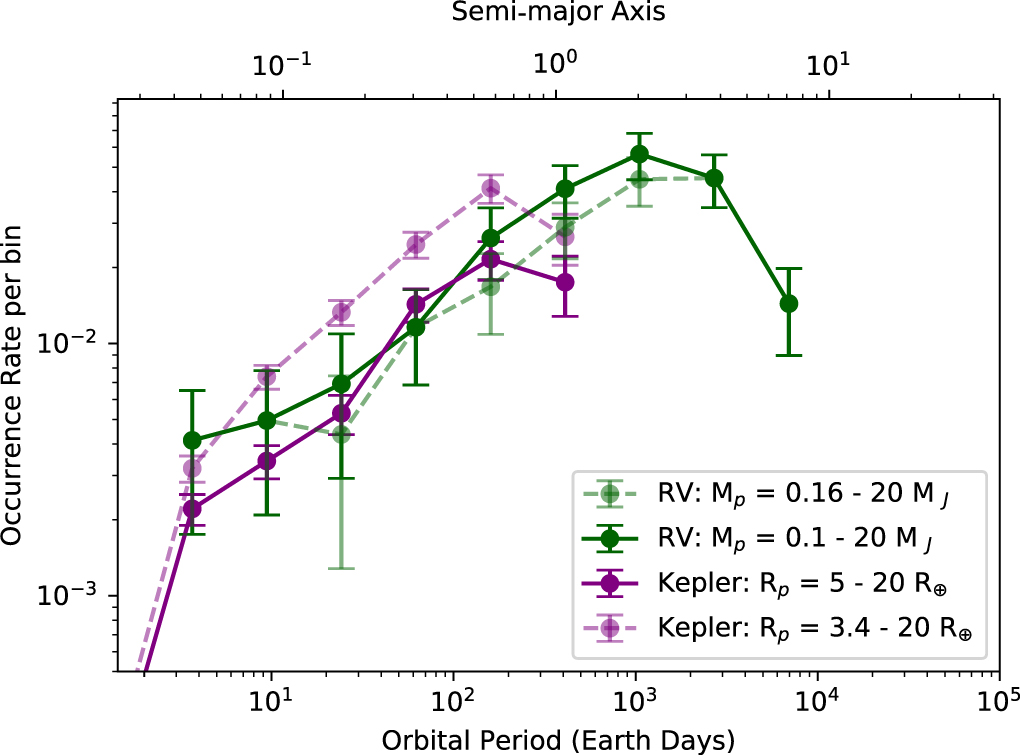
\includegraphics[width=0.8\textwidth]{Figure_Chap1/Fernandes2019_Figure02.jpg}
    \caption[Le nombre d'occurrence des exoplanètes détectées par la méthode des vitesses radiales et par la mission Kepler en fonction de la période orbitale et du demi-grand axe.]{Le nombre d'occurrence des exoplanètes géantes en fonction de la période orbitale (axe du bas) et du demi-grand axe (axe du haut) détectées par la méthode des vitesses radiales (ligne continue verte) et par la mission Kepler (ligne continue violette). Les courbes sont données pour plusieurs intervalles de masse et de rayon (lignes continues ou discontinues). Figure tirée de \cite{fernandes2019}.}
    \label{fig:Fernandes2019F2}
\end{figure}


%%%%%%%%%%%%%%%%
\subsubsection{De FIRSTv1 à FIRSTv2}

L'instrument \ac{FIRST} a été développé \citep{kotani2008} pour appliquer le masquage et le réarrangement de pupille fibré combiné avec un spectrographe, dans la gamme de longueurs d'onde du visible, selon le concept développé par Sylvestre Lacour pendant sa thèse \citep{lacour2010} à partir de l'idée proposée par Guy Perrin \citep{perrin2006}. La figure~\ref{fig:FIRSTv1Scheme} présente un schéma de principe de cet instrument. La pupille du télescope est divisée en sous-pupilles représentée par le miroir déformable segmenté (1) dont les segments bleus (au nombre de $9$) sont ceux dont la lumière est injectée dans les fibres optiques mono-modes (3) à l'aide d'une matrice de micro-lentille (2). Les fibres sont connectées aux fibres d'un V-Groove (la figure~\ref{fig:VGroove} présente des photographies de ce composant) de manière non-redondantes (4) où les sorties sont disposées sur une dimension (réarrangement de pupille). Les sorties du V-Groove sont dispersées par un spectrographe (5) et imagées sur la caméra dont une image est montrée (6). Ici les longueurs des fibres optiques ont dues être égalisées afin d'annuler les retard de phase entre les faisceaux des sous-pupilles au moment d'interférer dans le plan focal (6).

\begin{figure}[ht!]
    \centering
    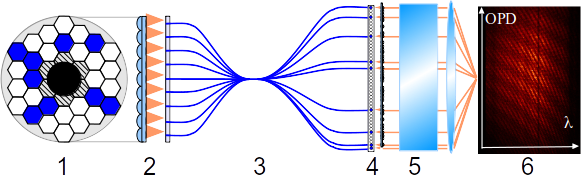
\includegraphics[width=0.8\textwidth]{Figure_Chap1/FIRSTv1Scheme_36Outputs_Fringes_b.png}
    \caption[Schéma de principe de FIRSTv1.]{Schéma de principe de FIRSTv1. La lumière se propage de gauche à droite, sur les composants suivants : (1) le miroir segmenté représenté avec l'obstruction centrale du télescope, (2) la matrice de micro-lentilles, (3) les fibres optiques monomodes, (4) le V-Groove pour le réarrangement de pupille, (5) le spectrographe et (6) la caméra. Crédit : Elsa Huby.}
    \label{fig:FIRSTv1Scheme}
\end{figure}

L'instrument a ensuite été intégré pour sa première lumière \citep{huby2012} sur le télescope de $3 \,$m Shane de l'observatoire Lick durant la thèse d'Elsa Huby \citep{huby2013these}. La figure~\ref{fig:FIRSTv1PupilMaskingA} présente le masquage de pupille utilisé sur \ac{FIRST} (à gauche) et leur réarrangement non-redondant à $1$ dimension à l'aide d'un V-Groove (à droite). Une image des réseaux de franges mesurée lors d'une observation de Véga ($\upalpha$ Lyr) est présentée sur la gauche de la figure~\ref{fig:FIRSTv1PupilMaskingB} sur laquelle l'axe vertical est l'axe des \ac{OPD}s et l'axe horizontal est l'axe des longueurs d'onde. Sur cette image on voit la superposition de $9 \times 8 / 2 = 36$ réseaux de franges donnant l'information de $36$ fréquences spatiales. Enfin, la partie droite de la figure~\ref{fig:FIRSTv1PupilMaskingB} présente la densité spectral de puissance (obtenue par la transformée de Fourier) de l'image précédente, sur laquelle on voit les pics de fréquences spatiales échantillonnées.

\begin{figure}[ht!]
    \centering
    \begin{subfigure}[t]{0.45\textwidth}
        \centering
        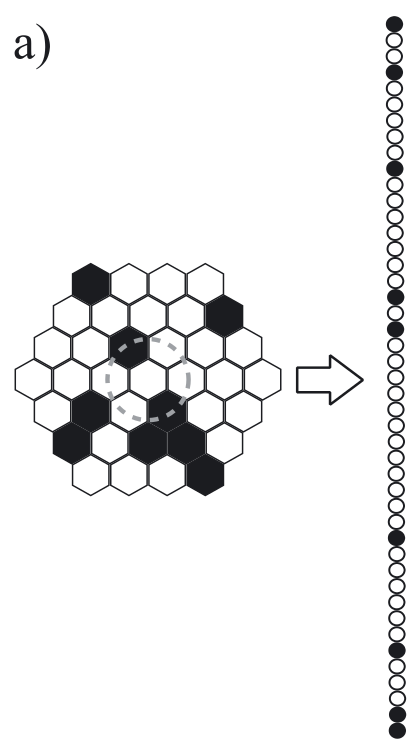
\includegraphics[width=0.7\textwidth]{Figure_Chap1/Huby2012_Figure2a.png}
        \caption{À gauche, la configuration des sous-pupilles choisies, à droite, la configuration 1-D choisie pour le réarrangement de pupille.}
        \label{fig:FIRSTv1PupilMaskingA}
    \end{subfigure}
    \begin{subfigure}[t]{0.45\textwidth}
        \centering
        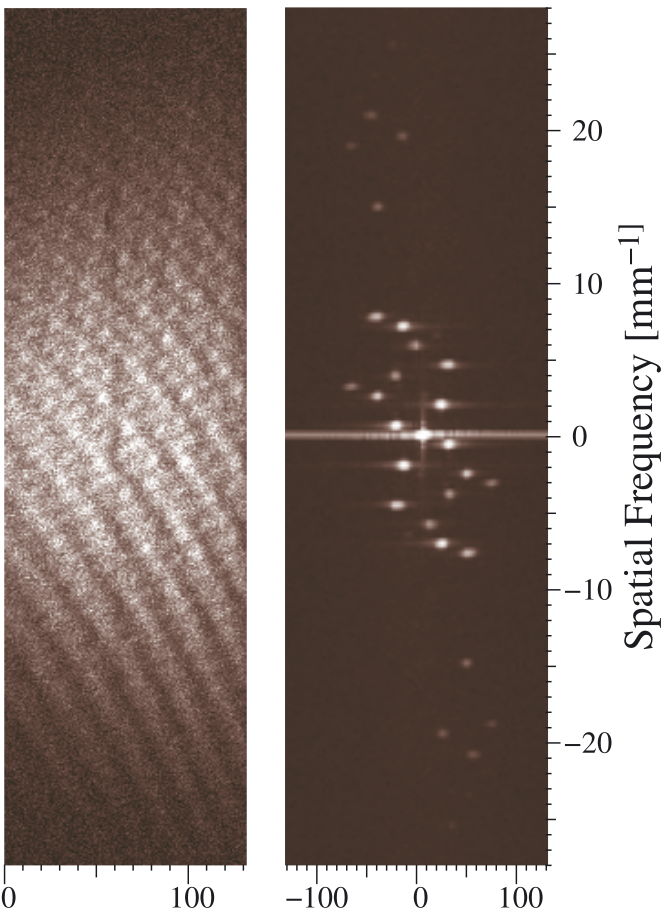
\includegraphics[width=0.9\textwidth]{Figure_Chap1/Huby2012_Figure3.png}
        \caption{À gauche, une image des réseaux de franges mesurée sur la caméra lors d'une observation de Véga, à droite la densité spectrale de puissance de cette image, montrant la répartition de l'échantillonnage du plan UV.}
        \label{fig:FIRSTv1PupilMaskingB}
    \end{subfigure}
    \caption[Expérience de masquage et de réarrangement de pupille de l'instrument FIRSTv1.]{Expérience de masquage et de réarrangement de pupille de l'instrument FIRSTv1, tiré de \cite{huby2012}.}
    \label{fig:FIRSTv1PupilMasking}
\end{figure}

De cette manière, les performances de ces techniques ont été démontrées durant la thèse d'Elsa Huby \citep{huby2013} à partir d'observations sur l'étoile multiple Capella ($\upalpha$ Aur) sur le télescope de $3 \,$m Shane de l'observatoire Lick. La séparation des deux composantes résolues par \ac{FIRST} est estimée à $50 \,$mas avec une précision de l'ordre de $1 \,$mas, ce qui est en-deçà du pouvoir de résolution du télescope ($58 \,$mas à $850 \,$nm). L'orbite d'une des deux composantes (l'autre étant centrée dans le champ de vue du télescope), est aussi reconstruite et est en accord avec les prédictions dans un intervalle de $1 \sigma$. Cela a aussi donné lieu à la première mesure du spectre du rapport de flux des deux composantes ($\sim 1$) aux longueurs d'onde $600 - 850 \,$nm avec une résolution spectrale de $\sim 300$. Des raies d'émission ont pu être identifiées (notamment la raie \ha, les bandes TiO et CN) et analysées en regard de simulations.

À la fin de sa thèse, Elsa Huby a participé à l'intégration de \ac{FIRST} sur la plateforme \ac{SCExAO} sur le télescope de $8 \,$m Subaru. Le concept est resté le même et cela a permis de bénéficier du plus grand miroir du Subaru afin d'augmenter le flux lumineux injecté dans l'instrument ainsi que son pouvoir de résolution, tout en bénéficiant de la correction extrême d'optique adaptative de la plateforme \ac{SCExAO} ainsi que la meilleure qualité de ciel (en terme de turbulence atmosphérique) à disposition sur Terre. Cela permet en conséquence d'acquérir des images interférométriques avec un temps d'exposition plus long et donc d'augmenter la sensibilité de l'instrument. Les premiers résultats et la démonstration de l'instrument sur ciel ont été publiés par Sébastien Vievard dans \cite{vievard2020a, vievard2022} afin de démontrer la faisabilité du concept sur un télescope faisant partie de la classe des télescopes d'une dizaine de mètres de diamètre avec un système d'optique adaptative extrême, grâce à de nouvelles observations sur le système Capella ($\upalpha$ Aur) amenant à la mesure de leur séparation et orientation.

Une réplique de cet instrument a été développée par Nick Cvetojevic sur le banc de test \ac{FIRSTv2} au laboratoire \ac{LESIA} (à Meudon) dans le but de tester de nouvelles solutions de recombinaison des sous-pupilles. Ce banc de test est amplement détaillé dans la section~\ref{sec:FIRSTv2Concept} mais je résume son principe ici. Il s'agit ici de recombiner indépendamment les faisceaux par paire en injectant les faisceaux des sous-pupilles dans un composant d'optique intégré, là où sur la première version les faisceaux interféraient sur le plan focal de l'instrument. Cette technologie est dite photonique car elle consiste en un bloc de verre dans lequel sont gravés des guides d'onde. Les faisceaux des n sous-pupilles y sont injectés, puis sont divisés en $\text{n} - 1$ sous-faisceaux pour être ensuite recombinés par paire. Enfin, les sorties de la puce sont connectées aux fibres d'un V-Groove, dont ses sorties (qui n'ont pas besoin d'être disposées de manière non-redondante comme précédemment) sont dispersées par un spectrographe et imagées sur un détecteur. La figure~\ref{fig:FIRSTv2FringesCameraB} présente les interférogrammes obtenus sur ce banc de test imagés par la caméra, pour la configuration de sous-pupilles montrée sur la figure~\ref{fig:FIRSTv2FringesCameraA} (pour plus de détails voir la section~\ref{sec:BaseConfig}). Chaque interférogramme est imagé sur des pixels différents sur le détecteur selon l'axe vertical, en étant dispersés selon l'axe horizontal. On note que ces interférogrammes sont pour une valeur d'\ac{OPD} et les franges sont mesurées sur l'axe des \ac{OPD}s grâce au miroir segmenté qui est contrôlable en piston. L'objectif avec cette nouvelle version est d'augmenter les performances en contraste et en sensibilité afin de permettre des mesures de systèmes exoplanétaires présentant de plus haut contrastes.

\begin{figure}[ht!]
    \centering
    \begin{subfigure}[t]{0.4\textwidth}
        \centering
        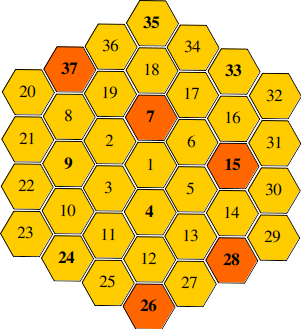
\includegraphics[width=0.9\textwidth]{Figure_Chap2/BaselineMap_37_7_26_15_28.png}
        \caption{Configuration des sous-pupilles choisies sur FIRSTv2.}
        \label{fig:FIRSTv2FringesCameraA}
    \end{subfigure}
    \begin{subfigure}[t]{0.55\textwidth}
        \centering
        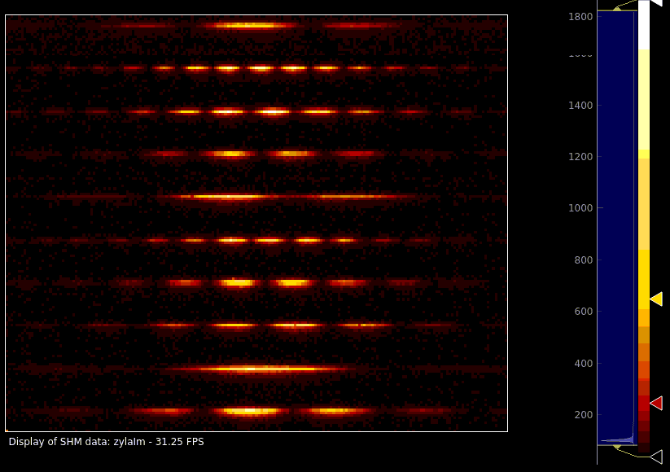
\includegraphics[width=0.9\textwidth]{Figure_Chap1/20220505_5TC_AY_InjectionOpti_Fringes_Meudon_crop.png}
        \caption{Image des interférogrammes sur la fenêtre de visionnage temps réel de la caméra de FIRSTv2 sur une source interne.}
        \label{fig:FIRSTv2FringesCameraB}
    \end{subfigure}
    \caption[Expérience de masquage et réarrangement de pupille de l'instrument FIRSTv2.]{Expérience de masquage et réarrangement de pupille de l'instrument FIRSTv2.}
    \label{fig:FIRSTv2PupilMasking}
\end{figure}

L'instrument \ac{GRAVITY} implémente ce même concept dans le proche infrarouge en recombinant les faisceaux des quatre télescopes du \ac{VLT} dans une puce photonique \cite{perraut2018}. Cela a mené à la première imagerie directe d'une exoplanète par interférométrie \citep{lacour2019} ce qui démontre la capacité de cette technique pour l'étude de systèmes exoplanétaires. Le développement de \ac{FIRSTv2} se fait dans les gammes de longueurs d'onde du visible afin d'améliorer les performances en résolution angulaire des mesures (celle-ci étant proportionnelle à la longueur d'onde) et de permettre la détection de la raie \ha~dans le spectre de protoplanètes, qui est probablement crucial pour la caractérisation des systèmes protoplanétaires, comme nous le verrons plus loin (section~\ref{sec:AccretionAlpha}).

Pour finir, \ac{FIRST} permet d'évaluer les futures performances de l'ensemble des techniques que nous avons vu ici sur les futurs \ac{ELT} de $> 30 \,$m de diamètre \citep{vievard2020b}. Un tel concept d'instrument sur cette classe de télescope permettrait d'atteindre un pouvoir de résolution angulaire égal à $\sim 2 \,$mas à $700 \,$nm, sur des systèmes avec un contraste allant jusqu'à $10 ^{-6}$. Cela augmenterait le nombre de candidats d'exoplanètes au champ de l'imagerie directe mais aussi à d'autres domaines d'études comme les centre actif des galaxies dans le visible.


%%%%%%%%%%%%%%%%
\subsubsection{L'apport de ma thèse au projet FIRST}

Le travail de ma thèse s'inscrit dans la continuité du développement de la réplique de \ac{FIRST} au laboratoire à Meudon. L'objectif est de tester en laboratoire la technologie d'optique intégré pour la recombinaison interférométrique des sous-pupilles. Cette technologie dans les gammes de longueur d'onde du visible est nouvelle dans le domaine de l'astronomie. En effet, elle a été développée et optimisée ces derniers décennies dans le domaine des télécommunications en infrarouge et son adaptation dans le domaine du visible nécessite de nombreuses années de développement et de test. J'ai ainsi caractérisé deux technologies différentes de composants d'optique intégré, présentés dans la section~\ref{sec:FIRSTv2Concept}, dans laquelle je présente toute l'expérience \ac{FIRSTv2}. 

De plus, une partie de mon travail de thèse a été de développer le logiciel de contrôle afin de le restructurer pour l'améliorer et d'ajouter de nouvelles fonctionnalités. Je présenterai ce travail dans la section~\ref{sec:ControlSoftware}. Ensuite, j'ai travaillé sur le développement du programme de traitement et d'analyse de données (section~\ref{sec:DataReduction}). Ce programme permet d'analyser des données acquises sur une source de type protoplanétaire que j'exposerai dans la section~\ref{sec:Protoplanetes}. J'ai alors démontré pendant ma thèse, la capacité de l'instrument \ac{FIRSTv2} à détecter une telle cible en intégrant au banc de test un système de sources lumineuses simulant une protoplanétaire compagnon d'une étoile (section~\ref{sec:SystBinaire}), en acquérant des données interférométriques sur celle-ci et en les traitant avec le programme développé pour l'occasion. Il s'agissait également d'implémenter pour la première fois sur le projet \ac{FIRST} la mesure des phases différentielles, qui est une observable particulièrement bien adapté à la détection de système protoplanétaire. Je présenterai les résultats de ces mesures dans la section~\ref{sec:BinaryCharac}. 

Enfin, La dernière partie de ma thèse a été l'intégration des puces photoniques sur la plateforme \ac{SCExAO} au télescope Subaru, pour la prise de données sur ciel lors de la première lumière de \ac{FIRSTv2}, que je présenterai dans la section~\ref{sec:FIRSTv2Subaru}. Lors de cette première lumière j'ai aussi eu l'occasion de déployer le logiciel de contrôle que j'avais développé et tester en laboratoire, à Meudon.


%%%%%%%%%%%%%%%%%%%%%%%%%%%%%%%%
\subsection{L'observation des systèmes protoplanétaires}
\label{sec:Protoplanetes}

%%%%%%%%%%%%%%%%
\subsubsection{La formation planétaire}

La variété des exoplanètes jusqu'alors détectées permet d'étudier des conditions physiques, astrométriques et chimiques différentes, constituant une source d'informations pour la compréhension des systèmes planétaires. Notamment, l'étude de leur évolution au cours du temps retient notre attention ici et est possible en étudiant différents systèmes d'exoplanètes se trouvant à différents stades de leur formation. 

Tout d'abord, l'étoile centrale se forme par effondrement de matière au sein d'un nuage de gaz, dominé par de l'hydrogène moléculaire. Lorsqu'un corps de quelques masses de Jupiter est formé, la densité y est suffisante pour qu'il y ait un état d'équilibre hydrostatique dans lequel la force de gravité compense la force de pression de la matière. Tout en s'effondrant sur l'étoile, le nuage de gaz acquiert un moment cinétique dominant et, en conséquence, se répartit sur un disque en rotation par effet centrifuge, ce qui explique que l'on retrouve les planètes et beaucoup de corps diverse du système solaire sur un même plan (l'écliptique). Ce disque protoplanétaire \citep{williams2011} se forme rapidement, en moins de $10 \,$kyr et est à des températures telles qu'il est observable dans les grandes longueurs d'ondes millimétriques à infrarouge. La figure~\ref{fig:DiskEvo} est une schématisation des étapes majeures de l'évolution de ce disque. L'étoile est totalement formée en $0.5 - 1 \,$Myr et induit sur le disque des rayonnements \ac{UV} qui ont pour effet d'évacuer tout le gaz de la partie interne du disque vers les plus lointaines orbites en l'espace de $\sim 0.1 \,$Myr (figure~\ref{fig:DiskEvo} (a), (b) et (c)). Jusqu'à environ $10 \,$Myr, le disque est encore protoplanétaire et est optiquement épais (la lumière visible ne s'échappe pas de l'intérieur du disque). Il contient encore du gaz primordial ainsi que de la poussière mais des intervalles vides se forment déjà, dû à la présence de protoplanètes. Entre $\sim 10 \,$Myr et $\sim 100 \,$Myr le disque est appelé disque de débris \citep{wyatt2008} car il ne contient plus du tout de gaz, qui a été accrété par les planètes, et il est constitué de poussières de seconde génération, provenant des nombreuses collisions d'astéroïdes et de planétésimaux (figure~\ref{fig:DiskEvo} (d)). L'âge maximal typique d'un disque de débris est de quelques $100 \,$Myr. Il est possible d'étudier ces détails des systèmes planétaires via les mesures de leur spectre électromagnétique. En effet, selon la taille des grains de poussières (qui augmente avec le temps) le rayonnement détecté évoluera vers les courtes longueurs d'ondes. De plus, les disques protoplanétaires, dans leurs premiers stades d'évolution, sont optiquement épais et l'étude de la répartition spectrale d'énergie permet d'inférer dans quelle mesure le disque modifie le spectre de l'étoile centrale.

\begin{figure}[ht!]
    \centering
    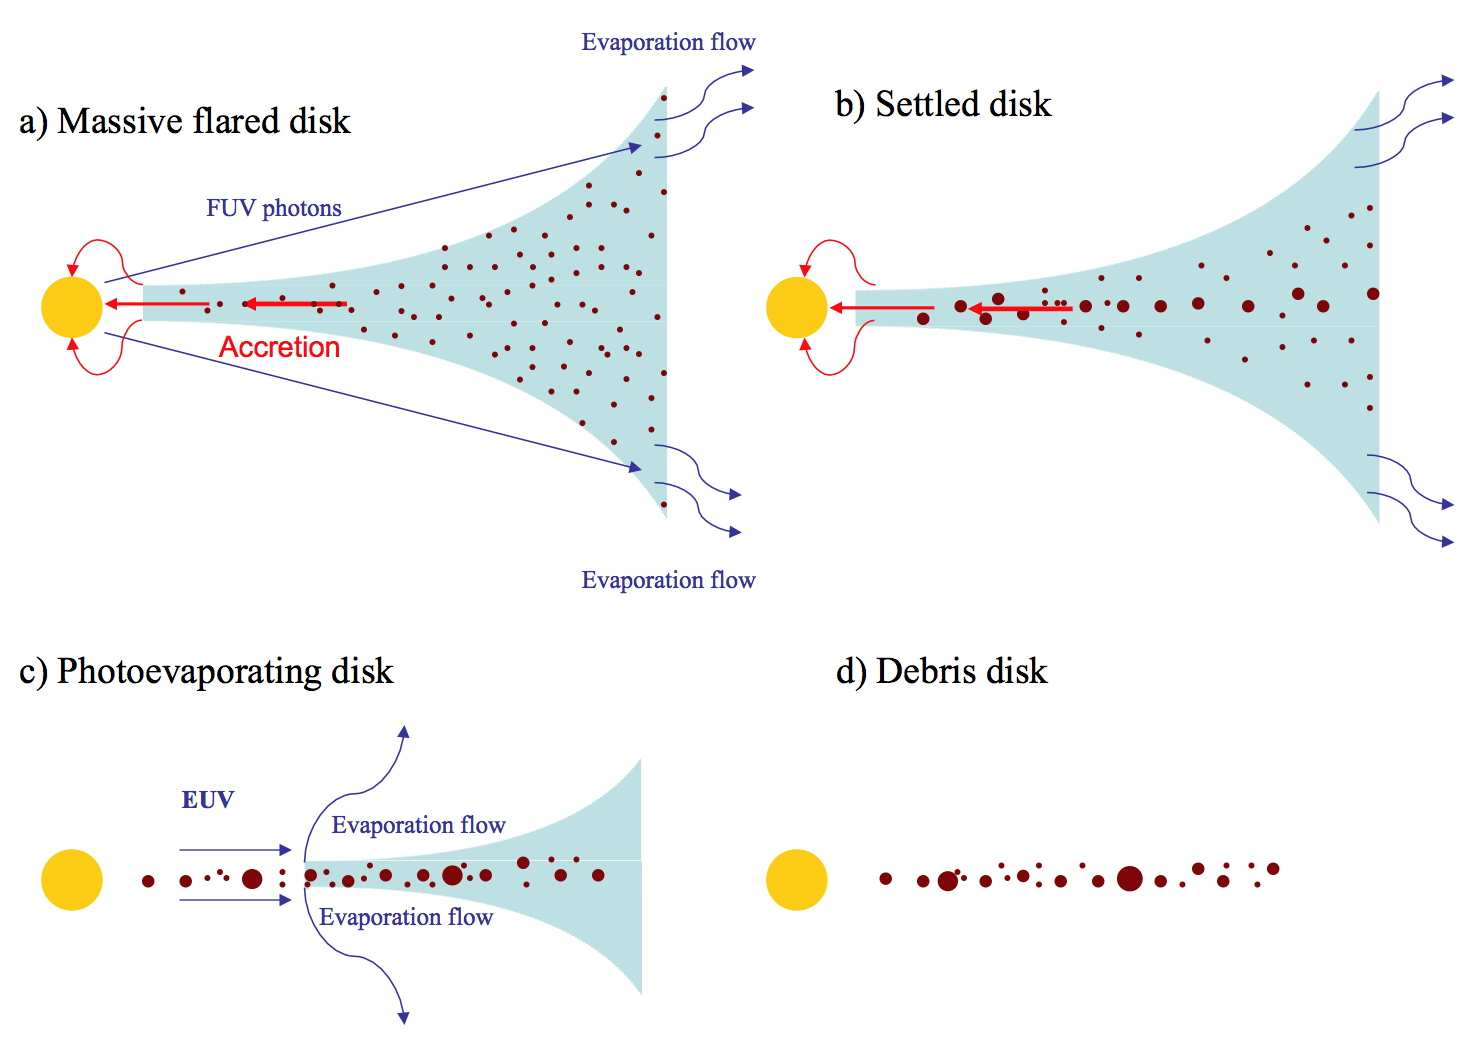
\includegraphics[width=\linewidth]{Figure_Chap1/Williams2011_Fig06_PlanetaryDiskEvolution.png}
    \caption[Évolution typique d'un disque protoplanétaire.]{Évolution typique d'un disque protoplanétaire, tiré de \cite{williams2011}. Le gaz est représenté en bleu et les poussières en marron. (a) Le disque dans son stade d'évolution primitif ($0-1\,$Myr) perd de la matière par accrétion sur l'étoile et photo-évaporation par les rayonnements \ac{UV} émis par l'étoile. (b) Les grains de poussières s'agglomèrent en débris de plus en plus gros tout en se répartissant sur un même plan. (c) L'étoile a fini de se former et le disque interne est dépourvu de gaz, devenant optiquement fin en quelques $0.1 \,$Myr. (d) Les plus petits grains de matière se font soit retirer par pression de radiation soit sont accrétés par les planètes et il ne reste que les planétésimaux au sein du disque, qui devient de plus en plus difficile à détecter, en l'espace de quelques $100 \,$Myr.}
    \label{fig:DiskEvo}
\end{figure}

Dans le même temps, on identifie $3$ stades d'évolutions des exoplanètes observées, pendant lesquels les exoplanètes sont nommées :

\begin{enumerate}
    \item protoplanètes lorsque le système est âgé de moins de $4 \,$Myr, ce sont les exoplanètes qui m'intéressent dans le cadre de mon projet de thèse, elles sont toujours en formation et accrètent de la matière, au sein du disque protoplanétaire et ont une forte émission dans la raie \ha~(comme on le verra plus en détails dans la section~\ref{sec:AccretionAlpha});
    
    \item jeunes planètes géantes lorsque le système est âgé de $4 \,$Myr à $100 \,$Myr, sont au sein d'un disque de débris, elles n'accrètent plus de matière mais ont une température assez élevée ($\sim 700 - 1700 \,$K) pour émettre un rayonnement thermique visible et infrarouge et font partie du groupe d'exoplanètes les plus détectées en imagerie directe (e.g. Beta Pictoris b \citep{lagrange2010});
    
    \item planètes complètement formées lorsque le système est âgé de plus de $100 \,$Myr, constituant la grande majorité des exoplanètes connues et sont trop froides pour rayonner dans le visible (elles n'ont qu'un rayonnement infrarouge) comme sur les deux types d'exoplanètes précédemment cités, mais peuvent refléter suffisamment la lumière de leur étoile pour être détectées en imagerie directe (dans le visible).
\end{enumerate}

À ce jour, deux grandes théories existent pour décrire les mécanismes de formation planétaire. La première théorie est la formation par accrétion de matière (\ac{CA}, en anglais), pour la première fois énoncée dans \cite{safronov1972}. Les grains de poussières microscopiques se combinent pour former des corps de plus en plus gros : des astéroïdes, puis des planétésimaux (future planète). Enfin, si ces corps ont une masse d'au moins $10 \,$ M$_{\bigoplus}$, ils accrètent du gaz et deviennent des géantes gazeuses \citep{pollack1996}. Pour le système solaire, cela explique donc bien la présence de quatre planètes rocheuses dépourvues de gaz car il a été expulsé par le Soleil (comme expliqué dans le paragraphe précédent) sur les plus petites orbites ainsi que de planètes géantes gazeuses sur les orbites les plus lointaines et dont on soupçonne qu'elles contiennent un noyaux rocheux.

Bien que cette première théorie est la plus acceptée par la communauté, notamment pour expliquer la formation du système solaire, de récents travaux montrent qu'une deuxi\hyp{}ème théorie est plausible. Cette théorie fait appel à des processus d'instabilité gravitationnelle (\ac{GI}, en anglais) et est, par exemple, simulée dans \cite{nayakshin2017}. Ici, juste après la formation de l'étoile, des régions localisées dans le disque exoplanétaire se condensent par instabilités gravitationnelles en des corps de plusieurs fois la masse de Jupiter. Dans ces conditions, les grains de poussière sédimentent et forment un noyau rocheux central. Certaines simulations \citep{boley2010} montrent que ces amas se forment à $\gtrsim 50 \,$AU et migrent jusqu'aux basses orbites ($\sim 1 \,$AU), où ils perdent leur couche de gaz à cause des effets de marrée. Cela réussit aussi à expliquer la présence de petites planètes rocheuses aux orbites les plus proches du Soleil et des géantes gazeuses dotées de noyaux rocheux sur des orbites plus éloignées, où les effets de marrées ne sont pas suffisamment forts pour dissiper leur gaz.

Il est probable que les mécanismes de ces deux théories soient à l'oeuvre au cours de la formation planétaire. L'étude d'un plus grand nombre de systèmes protoplanétaires est donc indispensable pour contraindre ces théories.


%%%%%%%%%%%%%%%%
\subsubsection{L'accrétion de matière des protoplanètes}
\label{sec:AccretionAlpha}

Comme nous l'avons vu dans la section~\ref{sec:ImagerieDirecte}, l'imagerie directe permet l'étude de systèmes exoplanétaires encore jamais étudiés et permet une étude photométrique et spectroscopique de ceux-ci. Cette technique est adaptée à l'observation de protoplanètes car d'une part ce sont des systèmes jeunes et chauds donc ce sont les plus lumineux et d'autre part elle permet la mesure d'observables directement liées aux processus de formation planétaire.

L'une de ces observables qui nous intéresse est le spectre d'émission. En effet, l'accrétion de matière par un astre induit l'émission de raies associées à l'hydrogène dans le spectre mesuré. Lorsque le gaz, principalement composé d'hydrogène s'effondre sur une étoile ou une planète, il atteint des vitesses qui dépassent la vitesse du son locale. Le gaz génère en conséquence des ondes de choc augmentant la température de plusieurs milliers à plusieurs dizaines de milliers de Kelvins. À cette température, l'hydrogène est excité et émet les raies spectrales des bandes Lyman, Balmer, Paschen, etc. Ces émissions ont été simulées pour des proto-étoiles jeunes en accrétion à partir de modèles d'accrétion magnétosphérique \citep{muzerolle2001, natta2004, espaillat2008}, dans lesquels le gaz interagit avec le champ magnétique stellaire, permettant ainsi de déterminer les liens entre ces émissions et le taux d'accrétion. De telles émissions hydrogènes ont été mesurées pour un échantillon d'étoiles jeunes du nuage Lupus \citep{alcala2014, alcala2017}, permettant d'estimer leur taux d'accrétion de matière ainsi que les liens entre la géométrie des flux d'accrétion et le taux d'accrétion. Une étude similaire sur le taux d'accrétion de l'étoile PDS70 a aussi été conduite dans \cite{thanathibodee2020} en utilisant un modèle d'accrétion magnétosphérique. PDS70 est dite de type T Tauri (\ac{TTS}, en anglais) \citep{appenzeller1989}, qui définit les étoiles variables jeunes en formation, âgées de moins de $10 \,$Myr et appartenant à la pré-séquence principale (PDS70 est de type spectral K7). Comme beaucoup d'étoiles de type \ac{TTS}, PDS70 est dotée d'un disque de transition (stade d'évolution entre le disque protoplanétaire et le disque de débris). Ces disques se caractérisent par la présence d'orbites pratiquement vides contenant parfois des protoplanètes. Les taux d'accrétion ont plusieurs fois été calculés pour les étoiles de type \ac{TTS} \citep{natta2004, rigliaco2012, ingleby2013}.

Ces modèles d'accrétion de matière, initialement développés pour des étoiles jeunes et peu massives, ont été adaptés pour le cas de protoplanètes \citep{aoyama2018, thanathibodee2019}. Les difficultés d'une telle adaptation sont que les conditions d'accrétion sur les protoplanètes sont différentes de celles sur les étoiles : dans le cas des protoplanètes, (1) la température du gaz en accrétion est moins élevée (d'au moins un ordre de grandeur), (2) le milieu dans le voisinage de la protoplanète (le disque circumplanétaire) n'a pas les mêmes structures (c'est parfois un bras de gaz et de poussière \citep{boccaletti2020} approvisionnant en matière l'étoile encore en formation) et (3) les champs magnétiques locaux sont différents en intensité et en structure, entraînant des écoulements de gaz différents dans l'un ou dans l'autre des cas. Plus simplement, dans le cas des étoiles, le gaz est excité avant le choc supersonique et est ionisé après le choc car les champs magnétiques locaux sont assez puissants pour accélérer les écoulements alors que dans le cas des protoplanètes, le gaz n'est excité seulement qu'après le choc supersonique \citep{aoyama2019}.

L'étude des raies d'émissions hydrogène de Balmer, plus particulièrement la raie Balmer-$\alpha$ ($656.28 \,$nm), aussi appelée raie \ha, est un bon moyen d'estimer le taux d'accrétion de matière en cours sur les protoplanètes \citep{aoyama2019, marleau2022}. \ac{FIRSTv2} est conçu pour travailler dans cette gamme de longueur d'onde et ainsi détecter une raie \ha. C'est pour cela que dans la suite, je vais m'intéresser essentiellement aux travaux effectués sur la détermination du taux d'accrétion à partir de la mesure de cette raie.

Il est possible de contraindre le taux d'accrétion de matière de plusieurs manières différentes :

\begin{itemize}
    \item soit par l'utilisation de modèles magnétosphériques d'accrétion \citep{natta2004, ingleby2013, thanathibodee2019}, de modèles hydrodynamiques d'écoulement du gaz lorsqu'il s'effondre sur la protoplanète \citep{aoyama2018, aoyama2019, aoyama2020} ou de modèles d'émission par un bloc d'hydrogène à certaines conditions de température et de pression \citep{alcala2017, rigliaco2012}. Ces modèles sont ajustés aux spectres mesurés pour inférer la luminosité des raies d'émission ou directement la luminosité d'accrétion $log(L_{acc})$, qui sont alors utilisées pour calculer le taux d'accrétion avec les méthodes énoncées au point suivant.
    
    \item Soit par la mesure de l'intensité du pic \ha~qui permet de déduire la luminosité \ha~émise par la protoplanète connaissant sa distance à la Terre. Pour des étoiles de faibles masses ($< 0.1 \, M_{\odot}$), comme celles de type \ac{TTS}, la luminosité $log(L_{\text{\ha}})$ est reliée à la luminosité d'accrétion $log(L_{acc})$ par une relation affine selon $log(L_{acc}) = b + a \times log(L_{\text{\ha}})$. Enfin, le taux d'accrétion $\dot{M}$ est proportionnelle à la luminosité $L_{acc}$ libérée à l'impacte du flux d'accrétion sur la surface du corps selon une équation de chute libre provenant du modèle d'accrétion magnétosphérique \citep{gullbring1998}. \cite{wagner2018} applique cette méthode sur le système PDS70 et \cite{rigliaco2012} l'applique sur un échantillon d'une dizaine d'étoiles de type \ac{TTS} pour plusieurs raies d'absorptions de l'hydrogène. Il propose ainsi d'étalonner la relation entre l'émission \ha~et le taux d'accrétion pour ce type d'étoiles afin d'être employée à l'avenir sur le même type d'objet \citep{close2014}.
    
    \item Soit par la mesure de la largeur du pic \ha~émis. Plus précisément, de la largeur du pic à $10 \, \%$ de sa hauteur (W$_{10}$) qui est élargie en fonction du taux d'accrétion. En effet, \cite{natta2004, fang2009} suggèrent un seuil indiquant que des cibles qui présentent une largeur W$_{10}$ du pic \ha~inférieur à $4.4 \,$\AA (ou $200 \,$km.s$^{-1}$) n'accrètent pas de matière, dans le cas de corps de faibles masses de type stellaire (\ac{CTTS} ou \ac{WTTS}) ou géantes gazeuses. C'est aussi ce que montre les simulations de \cite{thanathibodee2019} (figure 4b) pour les protoplanètes du système PDS70 : il existe un seuil en dessous duquel (W$_{10} = 100 \,$km.s$^{-1}$) la largeur de l'émission \ha~ne dépend pas du taux d'accrétion $\dot{M}$ pour $\dot{M} < 10^{-8} \,$M$_{\text{Jup}}$.yr$^{-1}$. Les valeurs de seuil de taux d'accrétion diffèrent selon ces études car les modèles de simulations utilisés sont appliqués dans les premiers cas pour des corps stellaires de faibles masses et dans le deuxième cas pour des protoplanètes. Mais encore, le taux d'accrétion des protoplanètes du système PDS70 a pu être calculé à partir des largeurs W$_{10}$ mesurées sur les spectres obtenus sur l'instrument MUSE \cite{haffert2019, hashimoto2020}.
\end{itemize}

L'intérêt d'étudier les protoplanètes dans la raie \ha~est que le contraste de luminosité planète / étoile est bien moins élevé (d'un facteur $50$ à  $1000$ selon \cite{close2014}) ce qui augmente les chances de détection par \ac{FIRSTv2}. La mesure d'une telle raie permettrait à la fois de discriminer la présence d'une protoplanète qui, dans le reste de la bande spectrale, serait en dehors de la gamme de performances de l'instrument; mais aussi d'étudier son taux d'accrétion.

Dans les cas précédemment cités où le flux de la raie d'émission est utilisé, le taux d'extinction devra, dans certains cas, être pris en compte. En effet, étant donné que les protoplanètes se trouvent dans un disque de gaz et de poussières, ce dernier atténue son flux lumineux d'un facteur $A_R$. Pour le système PDS70, par exemple, la limite basse de ce taux a été estimé à $2.0 \,$mag et $1.1 \,$mag, respectivement pour la planète b et la planète a \citep{hashimoto2020}. Cette estimation a été faite à partir de modèles d'hydrodynamique simulant la quantité d'hydrogène moléculaire qui peut être liée à l'extinction de la poussière interstellaire. Ce taux d'extinction en \ha~de l'émission mesurée d'une protoplanète se fait donc en se basant sur nos connaissances du système, notamment sur la présence de gaz et de poussières (qui diffère pour un disque de transition par rapport à un disque plus jeune sans transition) qui peut être inféré par l'étude des spectres du système à d'autres longueurs d'ondes.

Il est aussi intéressant de noter que ce facteur d'extinction n'affecte que la hauteur des pics d'émissions et non leur largeur. On voit donc ici l'intérêt d'être capable de mesurer la largeur du pic \ha, notamment la largeur à $10 \, \%$ de la hauteur W$_{10}$, qui peut ainsi se faire sans se soucier de l'extinction au sein du disque. Mais pour cela, il est nécessaire de disposer d'une résolution spectrale suffisante. Par exemple, la raie spectrale mesurée sur PDS70b \citep{haffert2019} a une largeur à mi hauteur égale à FWHM$\, = 0.27 \pm 0.03 \,$nm et on souhaite mesurer six points sur cette raie, correspondant à un élément de résolution de $\delta\lambda = 0.09 \,$nm. Cela nécessite un spectrographe avec une résolution spectrale à $656.28 \,$nm de R$\, = 7292$. Actuellement, la résolution spectrale du spectrographe de \ac{FIRSTv2} est de R$_{FIRSTv2} = 4000$ (section~\ref{sec:InstruSpectro}) et ne permet donc pas de mesure fiable de la largeur d'une raie d'émission \ha~mais seulement sa mesure d'intensité.

Actuellement plusieurs systèmes semblent être pourvus de protoplanètes : 

\begin{itemize}
    \item les deux protoplanètes mises en évidence \citep{keppler2018, muller2018} autour de l'étoile PDS70, déjà mentionnée plus haut, qui présentent une émission \ha~plusieurs fois mesurée et étudiée. Je les présenterai plus amplement dans la section~\ref{sec:pds70}.
    
    \item Le système LkCa 15 présentant 3 protoplanètes observées, entre autres, par les instruments \ac{NIRC2} sur le télescope Keck-II \citep{kraus2012}, \ac{LMIRCam} sur le \ac{LBTI} et \ac{MagAO} sur le télescope Magellan Clay \citep{sallum2015}. De plus, lors d'observations avec l'instrument \ac{ISIS} sur le \ac{WHT} \citep{mendigutia2018} et avec \ac{CHARIS} sur le télescope SUBARU en combinaison avec \ac{NIRC2} sur le télescope Keck-II \citep{currie2019}, il a été mis en évidence qu'il se pourrait que ce soit le disque lui-même ou un compagnon Jovien qui émettent le rayonnement \ha et non des protoplanètes.
    
    \item La protoplanète Delorme 1 (AB)b \citep{eriksson2020, ringqvist2021} observée avec l'instrument \ac{MUSE} du \ac{VLT}.
    
    \item Le système MWC 758 observée avec un coronographe vortex installé sur l'instrument \ac{NIRC2} du télescope Keck-II \citep{reggiani2018} ainsi qu'avec l'instrument \ac{SPHERE} sur le \ac{VLT} \citep{cugno2019}.
    
    \item L'étoile T Cha observée par la technique de masquage de pupille avec \ac{NACO} sur le \ac{VLT} \citep{huelamo2011}.
    
    \item L'étoile HD 100546 observée par l'instrument \ac{NACO} du \ac{VLT} \citep{quanz2013, quanz2015}, par l'instrument \ac{GPI} du \ac{GST} \citep{currie2015, follette2017} et par \ac{SPHERE} sur le \ac{VLT} \citep{mendigutia2017}.% evidence for orbital motion is not yet clear \citep{rameau2017, sissa2018}
    
    \item Ainsi que l'échantillon de cibles étudié dans le cadre de la recherche de protoplanètes en accrétion \ac{GAPlanetS} avec l'instrument \ac{MagAO} \citep{follette2022}.
\end{itemize}
%  HD 169142 
%  Quanz et al. 2013b [https://ui.adsabs.harvard.edu/abs/2013ApJ...766L...2Q/abstract]
%  Biller et al. 2014 [https://ui.adsabs.harvard.edu/abs/2014ApJ...792L..22B/abstract]
%  Reggiani et al. 2014 [https://ui.adsabs.harvard.edu/abs/2014ApJ...792L..23R/abstract]

% Kraus & Ireland 2012 : mise en évidence d'une exoplanète dans une division d'un disque stellaire avec la technique de Non-Redundant Masking sur Keck-II


%%%%%%%%%%%%%%%%
\subsubsection{Le cas du système PDS70}
\label{sec:pds70}
% PDS70 is 5Myr old, mass of 0.87Ms
% PDS70b: sep of 180mas, semi-major axes 20au \citep{wang2021}, mass less than 10Mj
% PDS70c: sep of 240mas, semi-major axes 34au \citep{wang2021}, mass poorly constrained

% contraste de pds70 : $\sim 2.10^{-2}$

% lire aoyama 2020 sec 4.1.1 pour une review de pds70

% aoyama2019 : utilisation des simu de taux d'accrétion sur le cas pds70
% planete découverte en IR par \cite{keppler2018, muller2018}
% émission halpha de PDS70b mesurée par \cite{wagner2018} puis de PDS70c par \cite{haffert2019} (confirmation de b)
% Zhou et al. 2021

% e.g. \cite{rigliaco2012} étalonne une telle relation sur des étoiles de types \ac{TTS} et permet d'exprimer le logarithme de la luminosité d'accrétion $log(L_{acc})$ en fonction du logarithme de la luminosité \ha~$log(L_{\text{\ha}})$ selon une fonction affine selon : $log(L_{acc}) = 2.27 \pm 0.23 + (1.25 \pm 0.07) \times log(L_{\text{\ha}})$.

% haffert2019 calcule que les planetes b et c sont en résonance orbital 2:1 et comme suggéré par walsh2011, While the most massive planet Jupiter was formed first and was migrating towards the young Sun, the formation and subsequent faster inward migration of Saturn locked the two planets in a 3:2 mean motion resonance. This is thought to have reversed their, now coupled, migration direction outward towards their current orbits. Finding other systems, like PDS 70, in mean-motion resonance lends credibility to this formation scenario for our solar system.
% @article{walsh2011,
% 	doi = {10.1038/nature10201},
% 	url = {https://doi.org/10.1038%2Fnature10201},
% 	year = 2011,
% 	month = {jun},
% 	publisher = {Springer Science and Business Media {LLC}},
% 	volume = {475},
% 	number = {7355},
% 	pages = {206--209},
% 	author = {Kevin J. Walsh and Alessandro Morbidelli and Sean N. Raymond and David P. O{\textquotesingle}Brien and Avi M. Mandell},
% 	title = {A low mass for Mars from Jupiter's early gas-driven migration},
% 	journal = {Nature}
% }

% \citep{thanathibodee2019}
% formule avec l'intensité de la raie halpha, obtenue à partir de la comparaison de modèle magnétosphérique et des données du système PDS70 \citep{thanathibodee2019} : log(M) = (0.280 +- 0.002)log(Lhalpha) - (6.14+-0.02)
% Robust planet detections have been reported around the star
% PDS 70, a K7 star in the ∼5–10 Myr old Upper Sco
% association. PDS 70 is surrounded by a disk with an ∼80 au
% cavity (Riaud et al. 2006; Hashimoto et al. 2012, 2015; Keppler
% et al. 2018); it is also a pre-transitional disk (Espaillat et al.
% 2007), that is, a disk with a large cavity but with another
% optically thick disk in the innermost au from the star. This
% configuration was first identified by spectral energy distribution
% fitting (Dong et al. 2012; Hashimoto et al. 2012), and later
% confirmed by observations in the near-IR with SPHERE
% (Keppler et al. 2018) and in the submillimeter with ALMA
% (Long et al. 2018; Keppler et al. 2019). Keppler et al. (2018)
% reported the discovery of a companion at ∼22 au from the star
% in the gap between these two disks, confirmed by the 4σ
% detection of \ha emission at the location of the companion
% using MagAO narrow filters (Wagner et al. 2018). The
% companion, PDS 70b, has a mass between 5 and 14 Jupiter
% masses, as indicated by a comparison of magnitudes and colors
% with different model predictions. However, hydrodynamic
% simulations including PDS 70b on a circular orbit failed to
% reproduce the large width of the cavity, and an additional
% companion beyond the orbit of PDS 70b was suggested
% (Keppler et al. 2019). Indeed, using adaptive-optics-assisted
% integral-field spectroscopy with the Very Large Telescope
% (VLT)/MUSE, Haffert et al. (2019) detected Hα emission from
% PDS70b and reported additional Hα emission from a second
% planet, PDS70c.


\begin{comment}
%%%%%%%%%%%%%%%%%%%%%%%%%%%%%%%%
\subsection{L'observation de protoplanètes avec FIRSTv2}
\label{sec:ObsProto}
% Les mesures d'intensité du pic \ha~ainsi que sa largeur permettent de contraindre le taux d'accrétion mesuré (nécessitant des hautes résolution spectrales car width = $200 \,$ km.s$^{-1}$, impliquant resol spectrale de R$\, = 9000$ à la longueur d'onde \ha~pour avoir 6 points de mesure sur un pic).
% compagnon d'étoile en accrétion de matière, détecté avec la technique de SAM-interfero, HD 142527 B, in transtional disk  \citep{biller2012} + calculs de taux d'accrétion dans  \citep{close2014}
%  \citep{kraus2012} premières mesures avec technique de non redundant masking sur Keck-II, de la cible LkCa 15 (2Myr) montre une exoplanète dans un gap de disque circumplanétaire
% It should be noted that the community remains unsure of the formation mechanism of the PDS 70 planets. Bright and widely separated exoplanets such as the HR 8799 planets are often thought to have been formed by disk instability (Boss 2011). However, due to the presence of accretion on the PDS 70 planets, core accretion is one of the potential scenarios (as for the planets in our own solar system, e.g. Nesvorny, 2018). In the case of planets formed by core accretion, the accretion rate is expected to be at least as high as what is observed in the PDS 70 planets. The closer in time they are to the run-away accretion phase (that is when the planets acquire a critical mass to clear the gas and create a gap in the transitional disk), the more material the planets accrete (Fig. 1 top panel)
% Des forts taux d'accrétion favorisent CA


%%%%%%%%%%%%%%%%
\subsubsection{Étude de cas}
% sur la population des systèmes du nuage du Taureau :
% - intervalle sur les séparations angulaires des syst
% - intervalle sur les rapports de flux en halpha

% les instru actuels : MagAO (close 2018) et subaru (Jovanovic 2015) (Uyama 2020)
% n'observent des planètes qu'au-delà de 10AU (coronographe)
% avec masquage de pupille on peut sonder des zones de 1AU-10AU correspondant à une résolution angulaire entre 10 et 100mas

% meilleure resolution

%%%%%%%%%%%%%%%%
\subsubsection{Le signal attendu sur FIRSTv2 sur un système tel que PDS70}
\end{comment}
%%%%%%%%%%%%%%%%%%%%%%%%%%%%%%%%%%%%%%%%%%%%%%%%%%%%%%%%%%%%%%%%
\chapter{La réplique de FIRST en laboratoire : FIRSTv2}
\label{sec:FIRSTv2Concept}
\setcounter{figure}{0}
\setcounter{table}{0}
\setcounter{equation}{0}

\minitoc

\clearpage
\ac{FIRSTv2} est la deuxième version l'instrument \ac{FIRST} (installé sur le télescope Subaru) qui implémente une nouvelle solution de recombinaison interférométrique. Alors que la première version est un interféromètre multi-axial qui fait interférer la lumière des sous-pupilles du télescope dans un plan focal sur la caméra, dans la deuxième nous proposons de recombiner par paire ces sous-pupilles au sein d'un composant d'optique intégré.

Dans ce chapitre je présenterai le banc de test en laboratoire qui réplique \ac{FIRSTv2} dans sa globalité et je décrirai en détails les différents composants qui y sont intégrés. Je montrerai aussi la caractérisation des composants les plus cruciaux. Je décrirai également le logiciel de contrôle du banc dont j'ai poursuivi le développement et l'amélioration. Enfin, je montrerai les sous-pupilles que j'ai choisies de recombiner lors des prises de données présentées plus tard dans le manuscrit ainsi qu'une étude de stabilité des mesures de phases sur le banc.


%%%%%%%%%%%%%%%%%%%%%%%%%%%%%%%%
\section{Le banc de test à Meudon}

Le banc de test en laboratoire à Meudon (que je nommerai \ac{FIRSTv2} par simplification dans la suite) est une réplique de l'instrument \ac{FIRST}, qui est déjà installé au télescope de $8 \,$m de diamètre, le Subaru, sur le banc d'optique adaptative extrême \ac{SCExAO}. Ce banc de test a pour objectif de tester et valider les nouveaux développements expérimentaux, notamment des composants d'optique intégré pour la recombinaison interférométrique des faisceaux pour l'imagerie haut contraste de systèmes exoplanétaires.

\begin{figure}[ht!]
    \centering
    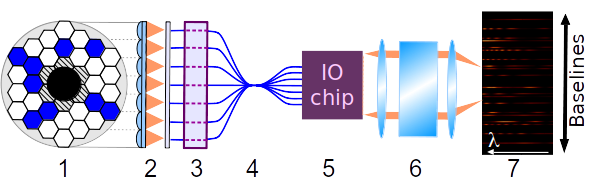
\includegraphics[width=\figwidth]{Figure_Chap2/FIRSTv2Scheme_20Outputs_Fringes_b.png}
    \caption[Schéma de principe du banc de test de FIRSTv2.]{Schéma de principe du banc de test de FIRSTv2. La lumière se propage de gauche à droite, sur les composants suivants : (1) le miroir segmenté représenté avec une obstruction centrale (non présente sur le banc de test de Meudon), (2) la matrice de micro-lentilles, (3) les lignes à retard (ODL), (4) les fibres optiques monomodes, (5) la puce d'optique intégrée, (6) le spectrographe et (7) la caméra.}
    \label{fig:FIRSTv2Scheme}
\end{figure}

La figure~\ref{fig:FIRSTv2Scheme} présente le schéma de principe de \ac{FIRSTv2}. Une source est injectée à gauche et parcourt tous les composants principaux suivants :

\begin{enumerate}
    \item le miroir segmenté, fabriqué par \textit{Iris AO Inc}, composé de $37$ segments hexagonaux contrôlables en piston, tip et tilt;
    \item la matrice de micro-lentilles fabriquée par \textit{SÜSS Optics MicroOptics}, qui applique le masquage de la pupille en focalisant les faisceaux des sous-pupilles dans les fibres optiques regroupées dans un toron fabriqué par \textit{Fiberguide Industries}\footnote{\url{https://www.molex.com/molex/products/group/fiberguide}};
    \item les lignes à retard fabriquées par \textit{Oz Optics}\footnote{\url{https://www.ozoptics.com/}}, que je nommerai par la suite \ac{ODL}, qui appliquent un aller-retour en air libre aux faisceaux injectés à l'aide d'un prisme réfléchissant contrôlable en position, afin de changer la longueur de chemin optique pour compenser les longueurs différentes entre les fibres optiques;
    \item les fibres optiques monomodes fabriquées par \textit{Thorlabs}, qui sont à maintient de polarisation et qui filtrent le front d'onde des faisceaux lumineux des aberrations optiques et permettent le réarrangement de pupille;
    \item la puce d'optique intégrée qui est un bloc de verre dans lequel ont été gravés des guides d'onde afin de recombiner par paires cinq faisceaux d'entrée;
    \item le spectrographe, composé d'un réseau holographique fabriqué par \textit{Wasatch Photonics} et donnant une résolution spectrale de $\sim 3\,200$ à $650 \,$nm;
    \item la caméra sCMOS, fabriquée par \textit{Andor}, sur laquelle sont imagés les interférogrammes pour chaque base sur l'axe vertical et en étant dispersés horizontalement.
\end{enumerate}

Tous ces composants seront plus amplement détaillés par la suite. De plus, la figure~\ref{fig:FIRSTv2BenchPhoto} montre une photographie du banc en laboratoire. Tous les composants sont numérotés et la source est injectée dans un V-Groove (1) (voir la figure~\ref{fig:VGroove}) qui est un composant alignant plusieurs fibres optiques (ici $8$ fibres) avec une séparation connue et qui peut être utilisé ici pour simuler une source protoplanétaire (voir la section~\ref{sec:SystBinaire}). La lentille (2) de focale égale à $300 \,$mm focalise le faisceau à l'infini. Ce dernier est réfléchi par le miroir plan (3) puis par le miroir en forme de D (4) avant d'atteindre le miroir segmenté (nommé aussi \ac{MEMS} par la suite) (5) selon une incidence quasi-normale. Les lentilles (6) et (7) de focales égales à $300 \,$mm et à $125 \,$mm, respectivement, forment un doublet afocal permettant un grandissement de $125 / 300 \simeq 0,42$ entre le diamètre du cercle inscrit des segments du \ac{MEMS} égal à $606,2 \,$\um~et le diamètre des micro-lentilles (8) égal à $250 \,$\um~($250 / 606,2 \simeq 0,41$). Les micro-lentilles (8) sont disposées sous forme d'une matrice et focalisent les faisceaux des sous-pupilles dans les fibres optiques monomodes disposées dans le toron (9). Les fibres optiques sont alors branchées sur les \ac{ODL}s (10). Les fibres d'entrées (à gauche de la puce sur la photographie) de la puce photonique (11) sont branchées en sortie de ces \ac{ODL}s et les fibres de sorties (à droite de la puce sur la photographie) sont branchées à un V-Groove (12) (disposant de $36$ fibres). Les sorties des fibres de ce V-Groove sont collimatées par un objectif de microscope (13) et sont enfin dispersées par un réseau holographique (14) et imagées par un doublet de lentilles (16) de focales égales à $150 \,$mm et à $80 \,$mm, sur la caméra (17). Un prisme de Wollaston peut être placé sur la plaque de métal (15). La partie spectrographique (éléments (13) à (16)) a été conçu et installé par Manon Lallement (voir plus de détails dans la section~\ref{sec:InstruSpectro}).

\begin{figure}[ht!]
    \centering
    \begin{subfigure}[t]{0.4\textwidth}
        \centering
        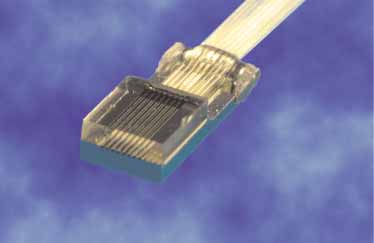
\includegraphics[width=\textwidth]{Figure_Chap2/VGroove_PigtailArray.png}
        \caption{V-Groove.}
        \label{fig:VGrooveA}
    \end{subfigure}%
    \begin{subfigure}[t]{0.4\textwidth}
        \centering
        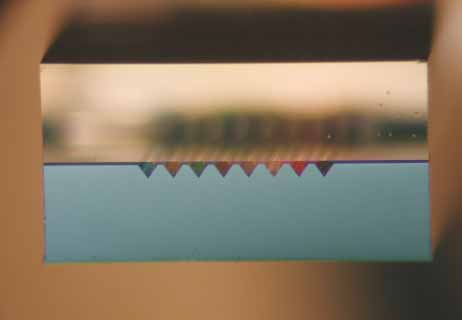
\includegraphics[width=0.94\textwidth]{Figure_Chap2/VGroove_EndFace.png}
        \caption{Face de sortie du V-Groove où l'extrémité des fibres sont placées dans des encoches en forme de V.}
        \label{fig:VGrooveB}
    \end{subfigure}
    \caption[Photographies d'un V-Groove.]{Photographies d'un V-Groove. Crédit : \textit{Oz Optics}.}
    \label{fig:VGroove}
\end{figure}

\begin{figure}[ht!]
    \centering
    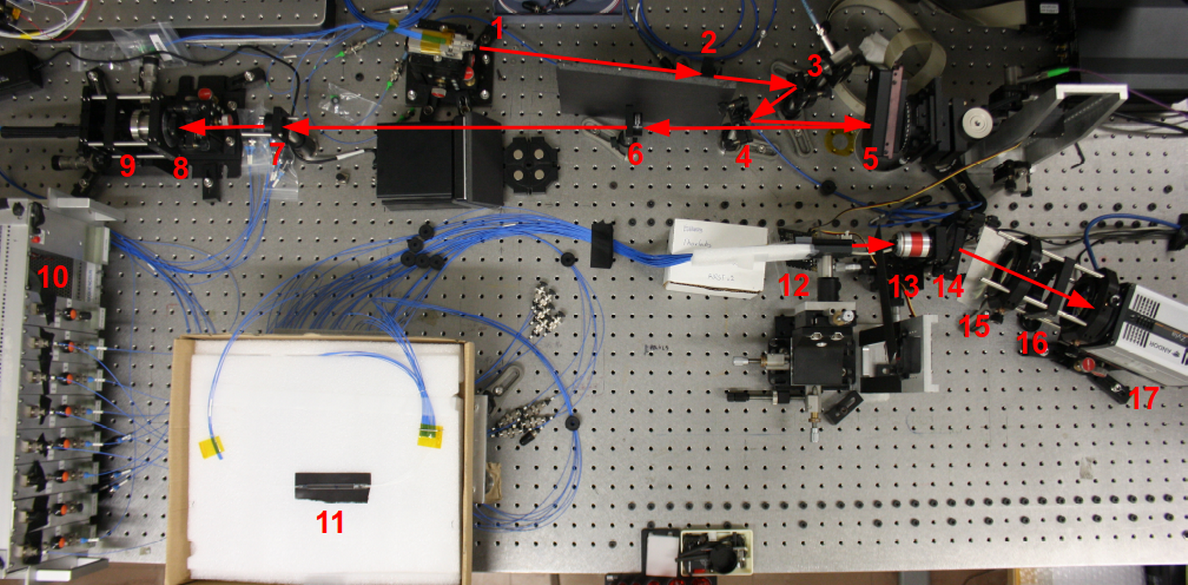
\includegraphics[width=\figwidth]{Figure_Chap2/20211215_FIRSTv2_MeudonBench_03.png}
    \caption[Photographie du banc de test FIRSTv2 à Meudon.]{Photographie du banc de test FIRSTv2 à Meudon. Tous les composants sont numérotés comme suit : (1) le V-Groove d'injection de la source, (2) une lentille, (3) un miroir plan, (4) un miroir D, (5) le MEMS, (6) et (7) le doublet de lentille, (8) la matrice de micro-lentilles, (9) le toron de fibres optiques, (10) les lignes à retard (ODL), (11) la puce d'optique intégrée, (12) un V-Groove, (13) un objectif de microscope, (14) le réseau holographique, (15) une plateforme pour disposer un prisme de Wollaston, (16) un doublet de lentille et (17) la caméra d'imagerie.}
    \label{fig:FIRSTv2BenchPhoto}
\end{figure}


%%%%%%%%%%%%%%%%
\subsection{Le miroir déformable Iris AO}

Le miroir déformable installé sur le banc de test de \ac{FIRSTv2} est fabriqué par \textit{Iris AO Inc} et je le nommerai par la suite \ac{MEMS}. La figure~\ref{fig:IrisAOMapA} est une photographie du miroir, sur laquelle on voit un des segments qui est coincé, les électrodes de lecture tout autour du miroir et la fenêtre d'ouverture noire. Le miroir dispose de $37$ segments hexagonaux identifiés sur la carte présentée sur la figure~\ref{fig:IrisAOMapB} (la carte est tournée de $+60\degree$ par rapport à la photographie) : le segment gris $17$ est le segment coincé inutilisable et les segments oranges sont ceux devant lesquels est placée une fibre optique du toron (voir plus de détails pour cela dans la section~\ref{sec:FiberInjection}). Lors du choix des cinq sous-pupilles à injecter dans la puce d'optique intégrée, les cinq segments correspondant ne peuvent donc être choisis que parmi ces $10$ segments oranges. Enfin, le cercle circonscrit de chaque segment mesure $700 \,$\um~de diamètre et celui de l'ensemble du pavage mesure $4,2 \,$mm de diamètre. Tous les segments, excepté le segment $17$, sont contrôlables en piston sur une plage de $\pm 1,5 \,$\um~et en tip-tilt sur une plage de $\pm 2\,$mrad.

\begin{figure}[ht!]
    \centering
    \begin{subfigure}[t]{0.4\textwidth}
        \centering
        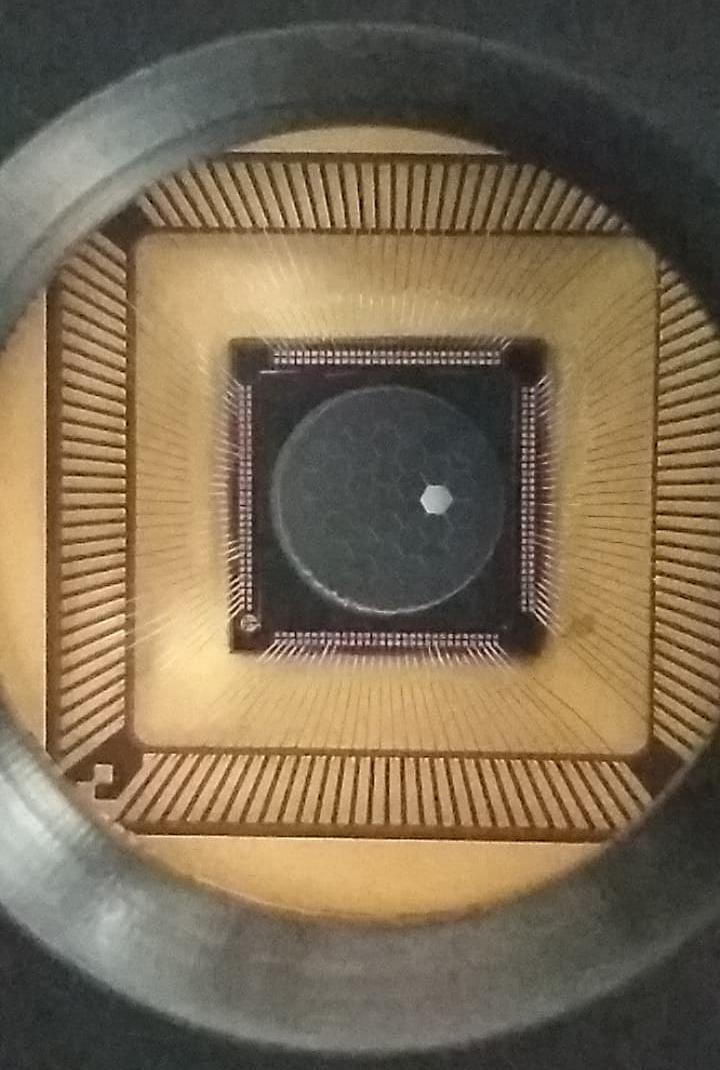
\includegraphics[width=0.8\textwidth]{Figure_Chap2/20191114_BrokenSegment_02.jpg}
        \caption{Photographie de la surface du miroir segmenté.}
        \label{fig:IrisAOMapA}
    \end{subfigure}\hspace{0.01\textwidth}
    \begin{subfigure}[t]{0.5\textwidth}
        \centering
        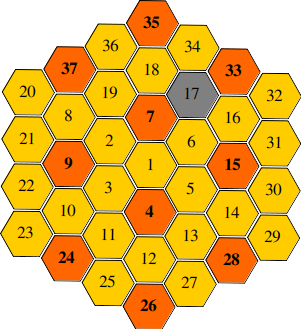
\includegraphics[width=0.8\textwidth]{Figure_Chap2/MemsMap_AllFibers.png}
        \caption{Carte d'identification des segments du miroir : en orange sont les segments devant lesquels est disposée une fibre optique et en gris est le segment cassé.}
        \label{fig:IrisAOMapB}
    \end{subfigure}
    \caption[Pavage du miroir segmenté \textit{Iris AO}.]{Pavage du miroir segmenté \textit{Iris AO}.}
    \label{fig:IrisAOMap}
\end{figure}


%%%%%%%%%%%%%%%%
\subsection{L'injection dans les fibres optiques}
\label{sec:FiberInjection}

%%%%%%%%
\subsubsection{Mise en oeuvre}

Les faisceaux des sous-pupilles sont injectés dans des fibres optiques monomodes à maintien de polarisation de type panda, de la gamme PM630-HP, fabriquées par \textit{Thorlabs}. Les fibres ont une ouverture numérique égale à $0,12$, un diamètre de mode égal à $4,5 \pm 0,5 \,$\um~(à $630 \,$nm) et leur cœur a un diamètre égal à $3,5 \,$\um. La propriété monomode de ces fibres permet de filtrer les aberrations du front d'onde du faisceau injecté, convertissant ainsi les variations de phases en variations d'intensité. Un ensemble de $19$ fibres est disposé dans un toron fabriqué par \textit{Fiberguide Industries}\footnote{\url{https://www.molex.com/molex/products/group/fiberguide}}, dont la photographie est montrée sur la figure~\ref{fig:InjectionCompB}, selon un motif hexagonal avec un espacement de $500 \,$\um~schématisé sur la figure~\ref{fig:InjectionCompC}. Cela explique la disposition des segments utiles (orange) sur la figure~\ref{fig:IrisAOMapB}.

\begin{figure}[ht!]
    \centering
    \begin{subfigure}{0.5\textwidth}
        \centering
        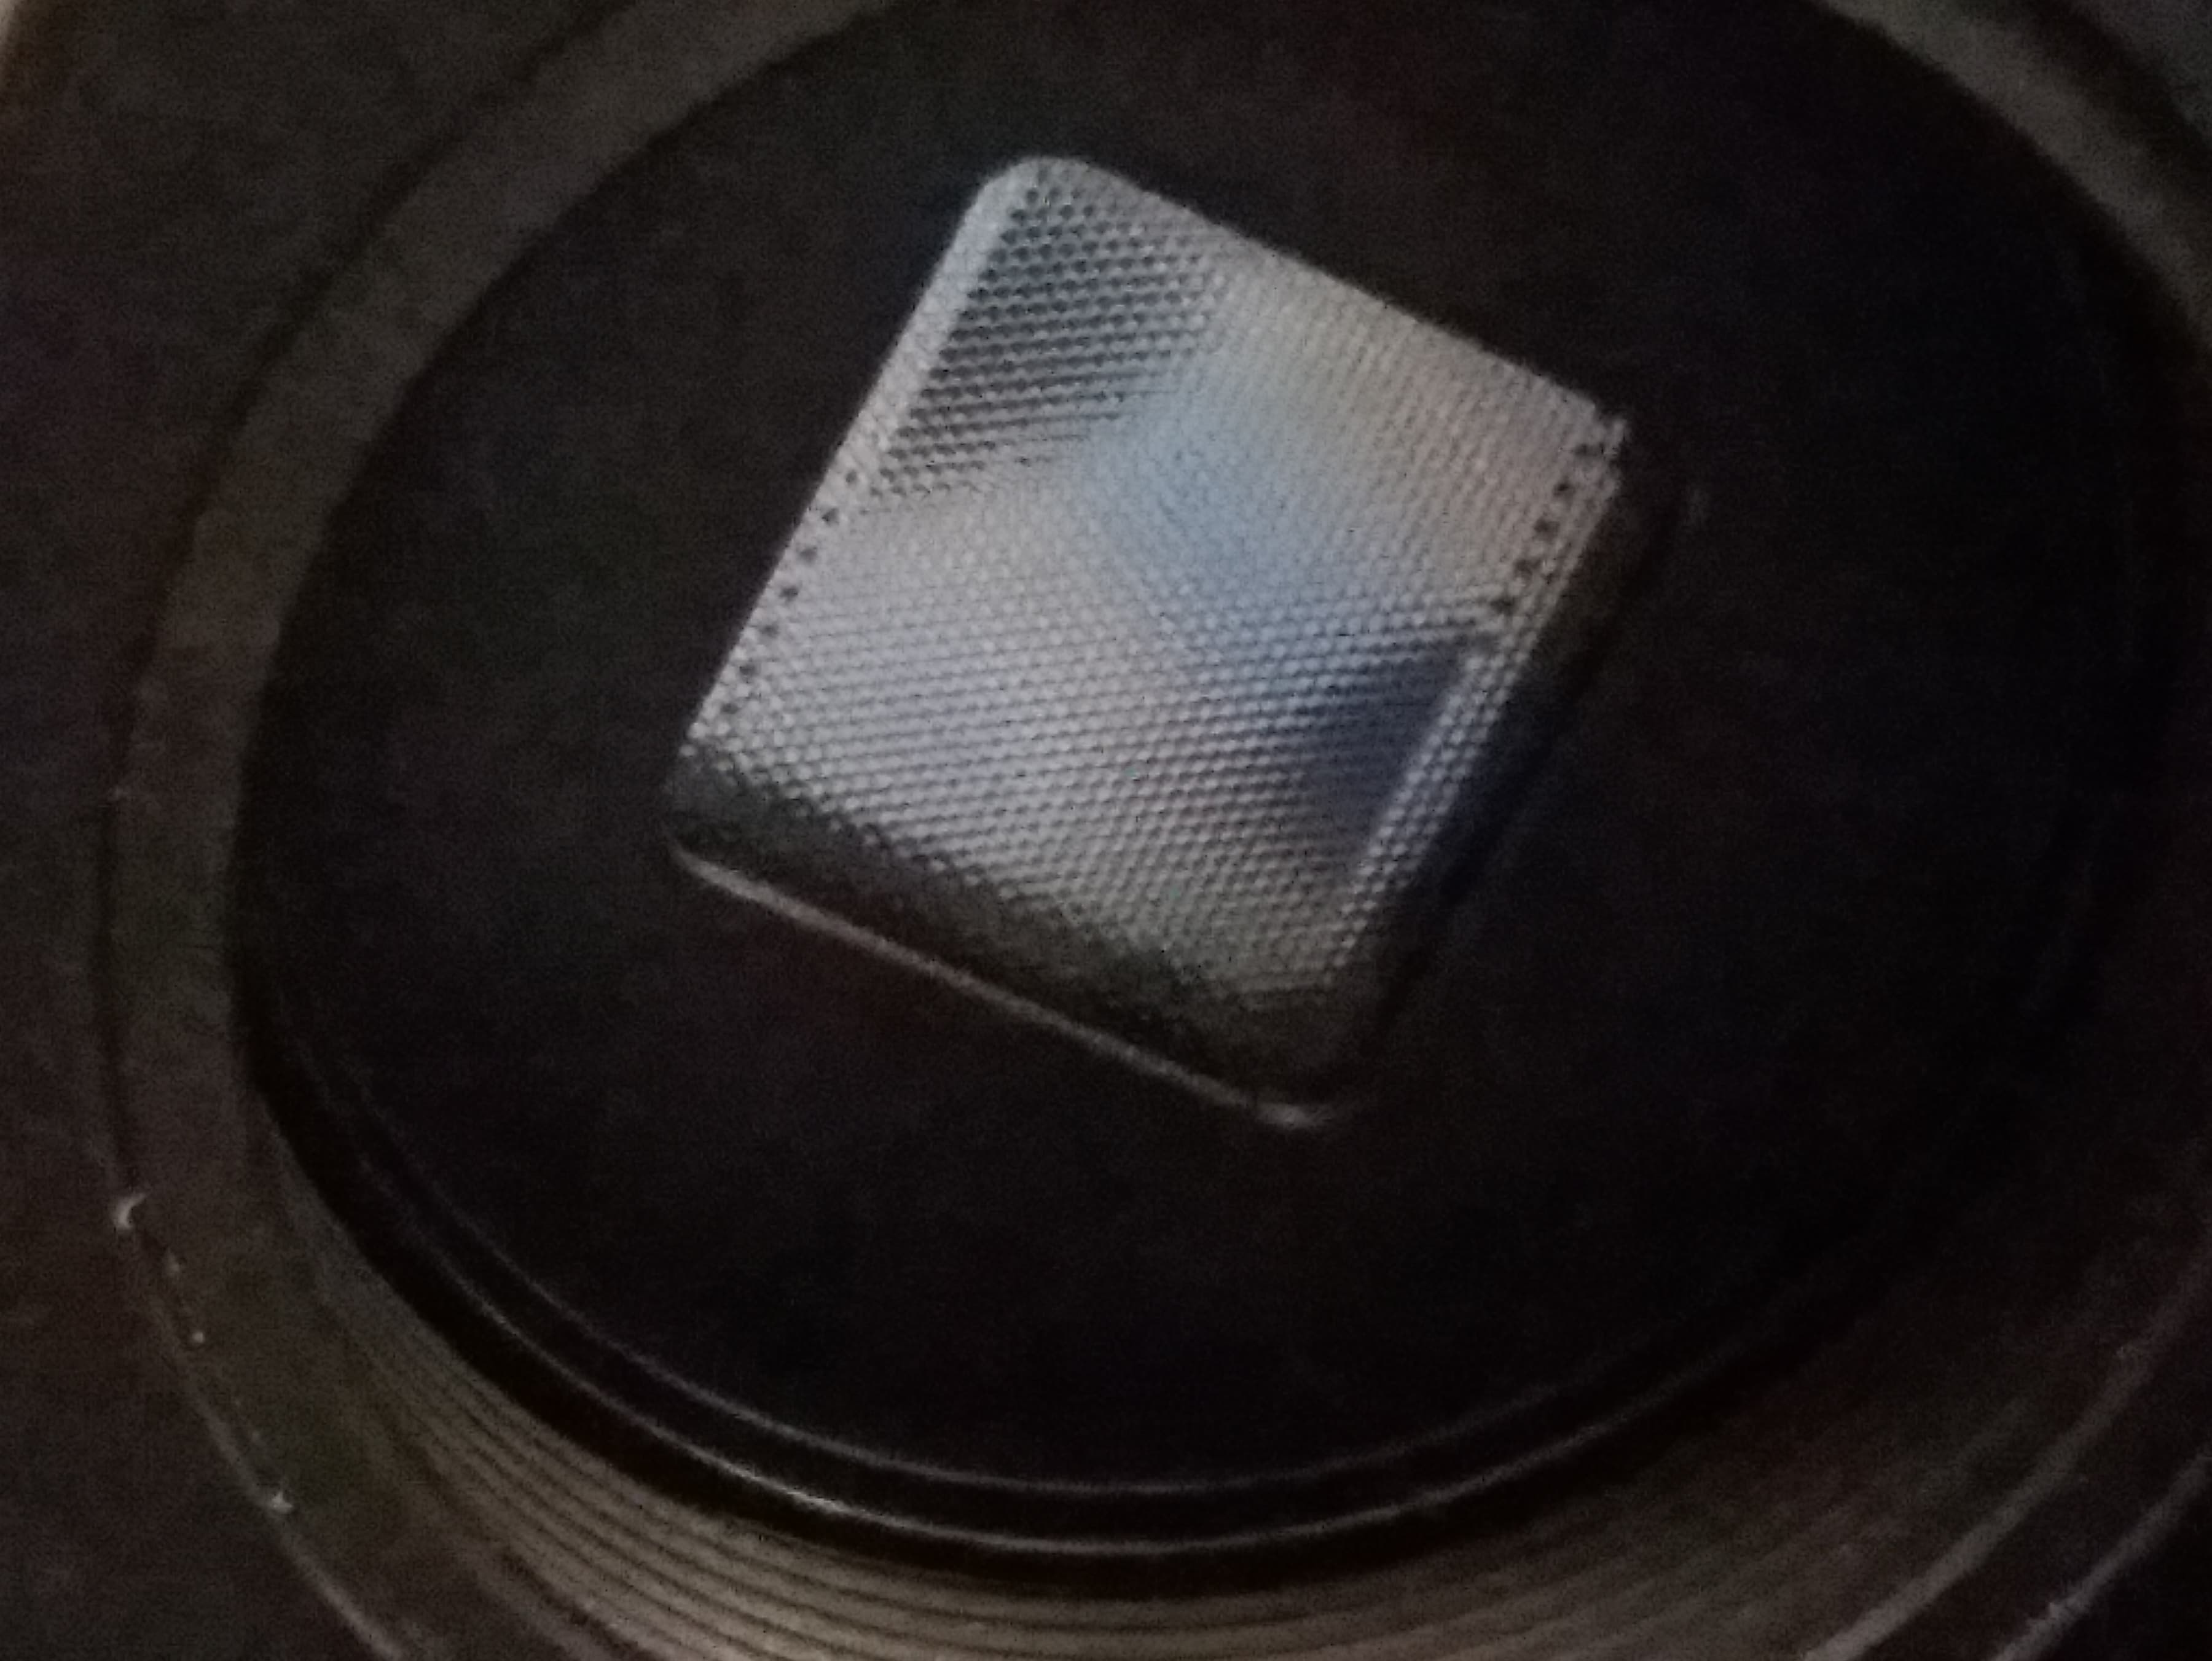
\includegraphics[width=0.9\textwidth]{Figure_Chap2/MicroLensArray.jpg}
        \caption{Photographie de la matrice de micro-lentilles utilisée pour diviser la pupille en sous-pupilles et focaliser les faisceaux dans les fibres optiques.}
        \label{fig:InjectionCompA}
    \end{subfigure}
    \begin{subfigure}[t]{0.5\textwidth}
        \centering
        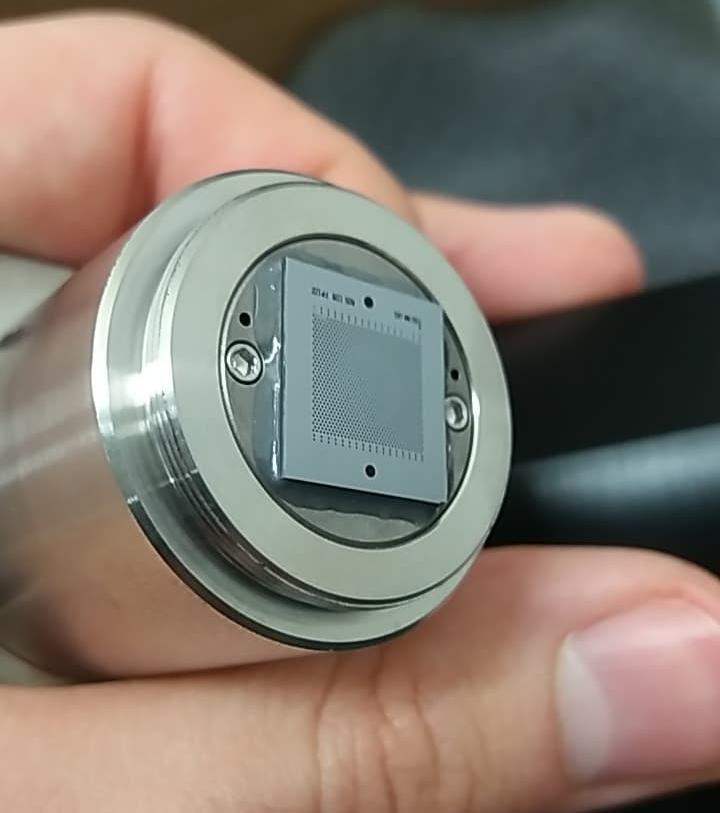
\includegraphics[width=0.8\textwidth]{Figure_Chap2/FiberBundle_Meudon03.jpg}
        \caption{Photographie du toron de $19$ fibres optiques utilisé pour l'injection des faisceaux des sous-pupilles.}
        \label{fig:InjectionCompB}
    \end{subfigure}%
    \begin{subfigure}[t]{0.5\textwidth}
        \centering
        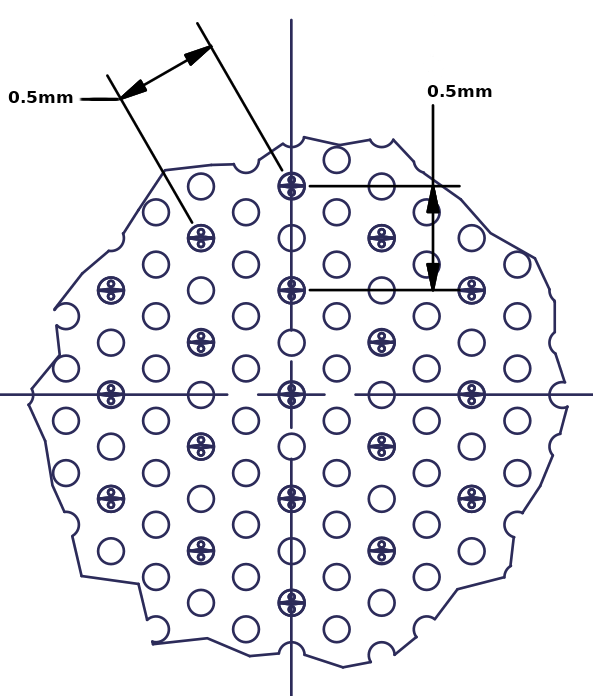
\includegraphics[width=0.8\textwidth]{Figure_Chap2/FiberBundle_Scheme.png}
        \caption{Schéma de la disposition des entrées des fibres optiques du toron. Crédit : \textit{Fiberguide Industries}.}
        \label{fig:InjectionCompC}
    \end{subfigure}
    \caption[Matrice de micro-lentilles et toron de fibres utilisés pour l'injection des faisceaux dans les fibres optiques.]{Matrice de micro-lentilles et toron de fibres utilisés pour l'injection des faisceaux dans les fibres optiques.}
    \label{fig:InjectionComp}
\end{figure}

Une matrice de micro-lentille, dont une photographie est présentée sur la figure~\ref{fig:InjectionCompA}, est disposé à $300 \,$\um~du toron. Les micro-lentilles ont une focale de $\sim 1 \,$mm et ont pour rôle de sous-diviser la pupille (masquage de pupille) et de focaliser les faisceaux des sous-pupilles dans les fibres optiques du toron. La matrice est placée dans le plan pupille conjugué du plan dans lequel est placé le miroir segmenté de telle sorte qu'une lentille, donc par extension une fibre optique, est alignée devant chaque segment. Les micro-lentilles ont un diamètre de $250 \,$\um~et ont donc un pas qui est la moitié du pas des fibres du toron. Un doublet de lentille de focales égales à $300 \,$mm et à $125 \,$mm adapte la taille des faisceaux provenant des segments du \ac{MEMS} de diamètre égal à $606,2 \,$\um~à la taille des micro-lentilles, par un grandissement d'un facteur $\sim 0,42$. Enfin, le faisceau de la source est en incidence quasi-normale sur le \ac{MEMS} pour déformer les sous-faisceaux le moins possible et maximiser la surface utile.


%%%%%%%%
\subsubsection{Procédure d'alignement}

Ce trio de composants nécessite d'être précisément aligné et toute la procédure qui suit est effectuée régulièrement car les dilatations mécaniques dues aux variations de température induisent un désalignement. Le toron de fibres est d'abord retiré du foyer des micro-lentilles et une caméra est installée à la place afin d'imager les segments du miroir à travers les micro-lentilles. Une telle image est montrée sur la figure~\ref{fig:MLAalignment} où l'on voit les faisceaux des sous-pupilles défocalisés à travers les micro-lentilles, elles-mêmes entourées des bords des segments hexagonaux. Le but est d'aligner les cercles au centre des hexagones et les lignes jaunes sont tracées sur l'image pour effectuer cet alignement sur toutes les micro-lentilles du champ à la fois.

\begin{figure}[ht!]
    \centering
    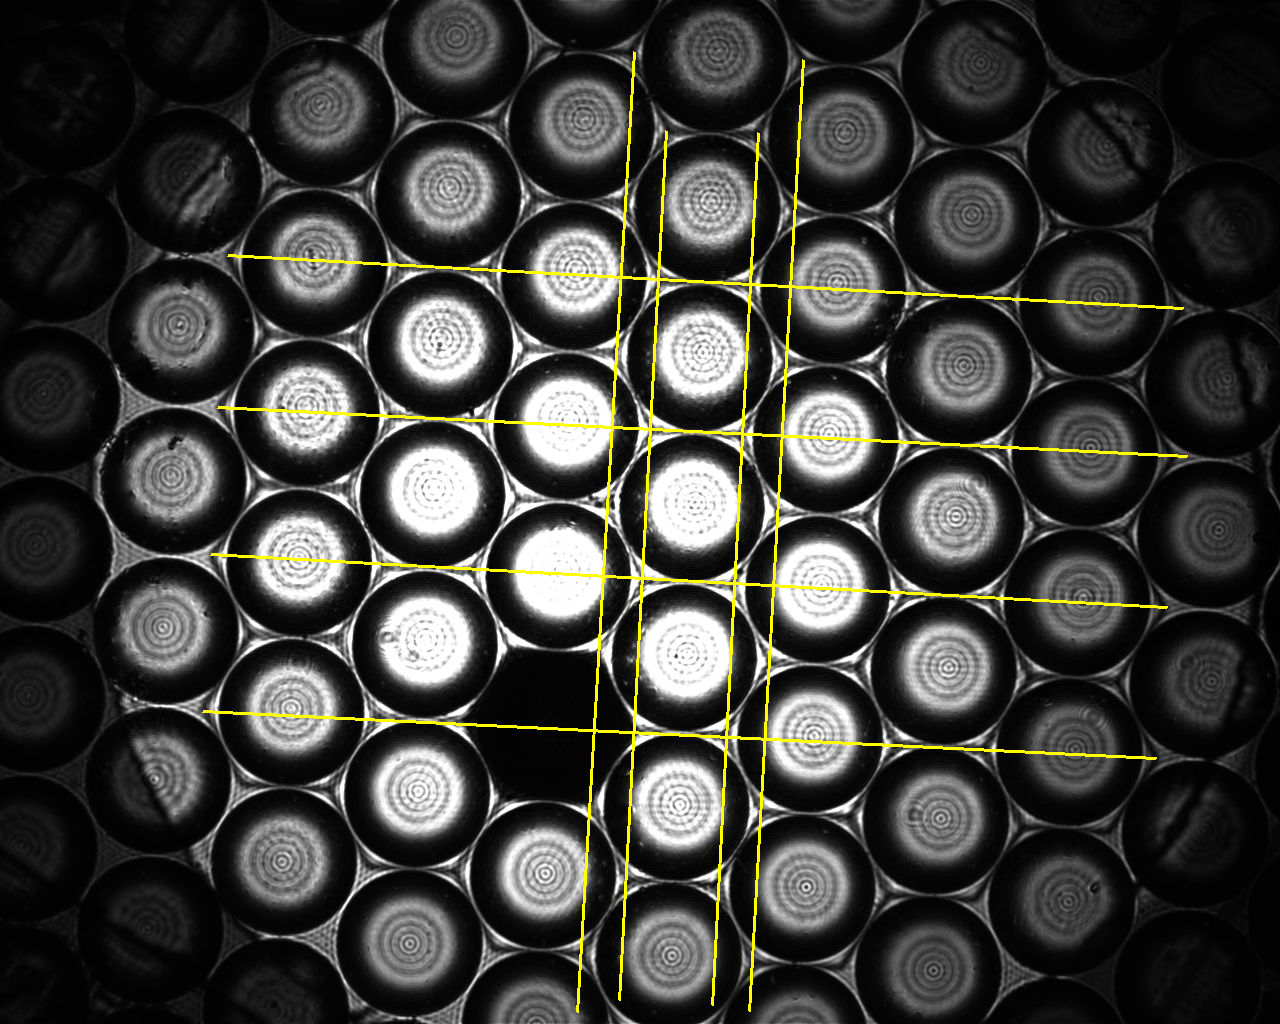
\includegraphics[width=0.7\textwidth]{Figure_Chap2/20191120_microlens_pupil_plane_2.jpg}
    \caption[Image du plan pupille après la matrice de micro-lentilles, prise lors de leur alignement par rapport au MEMS.]{Image du plan pupille après la matrice de micro-lentilles où les faisceaux des sous-pupilles sont défocalisés pour aligner les micro-lentilles par rapport aux segments hexagonaux du MEMS. On peut voir les hexagones entourant les micro-lentilles et les traits jaunes sont tracés pendant l'alignement pour aligner toutes les micro-lentilles du champ en même temps.}
    \label{fig:MLAalignment}
\end{figure}

Ensuite, la caméra est retirée et le toron est remis devant la matrice de micro-lentilles. Une source lumineuse est rétro-injectée dans les fibres optiques du toron et le faisceau réfléchi par le miroir segmenté est projeté sur un écran. Les segments sont déplacés en tip-tilt les uns après les autres afin d'identifier la position de la fibre illuminée par rapport au \ac{MEMS} et le toron est déplacé sur ses axes X et Y. Pour finir, la bonne position du toron sur son axe Z est trouvée en focalisant l'image par une des micro-lentilles de la source rétro-injectée.


%%%%%%%%
\subsubsection{Optimisation de l'injection}
\label{sec:OptiInj}

Une procédure programmée dans le logiciel de contrôle du banc permet d'optimiser l'injection des faisceaux des sous-pupilles dans les fibres optiques, en contrôlant les segments du \ac{MEMS} en synchronisation avec la caméra. Pour ce faire, les segments sont un à un déplacés en tip et en tilt sur un quadrillage dont la taille et le pas sont donnés en paramètres d'entrée de la procédure. Chaque segment quadrille la zone pendant que les autres sont mis en bout de course (à $2 \,$mrad) pour ne pas injecter de lumière. Pour chaque nouvelle position du segment, une image est prise sur la caméra et le flux total sur les sorties illuminées est calculé. Une carte de ces valeurs de flux est construite en fonction des positions de tip et de tilt pour déduire les coordonnées pour lesquelles le maximum de flux est mesuré, à l'aide d'un ajustement d'une fonction gaussienne. 

La figure~\ref{fig:OptiInj} est une capture d'écran de l'ordinateur de contrôle du banc de test et montre le résultat d'une optimisation de l'injection. En haut à gauche on peut voir les cinq cartes de transmission des cinq fibres tracées côte à côte, pour un intervalle de tip et de tilt de $\pm 2 \,$mrad avec un pas de $0.25 \,$mrad. Chacune de ces cartes présente un profil quasi-gaussien, correspondant à la convolution de la fonction d'étalement du point (\ac{PSF}) du faisceau injecté par le mode de la fibre optique. Une fonction gaussienne est alors ajustée à ces cartes pour inférer les positions qui maximisent les flux et sont enregistrées afin d'être ré-utilisées par la suite pour optimiser le flux injecté avant chaque nouvelle prise de données. En haut à droite de l'écran est affichée la carte de phase du \ac{MEMS} avec les cinq segments sur les positions qui optimisent le flux. En bas à droite est montrée l'image en temps réel de la caméra, sur laquelle on peut voir des franges d'interférences sur dix bases (axe vertical), dispersées horizontalement et dont les flux sont égalisés. On peut voir en arrière plan les terminaux de commandes des différents composants (voir la section~\ref{sec:ControlSoftware} pour plus de détails).

\begin{figure}[ht!]
    \centering
    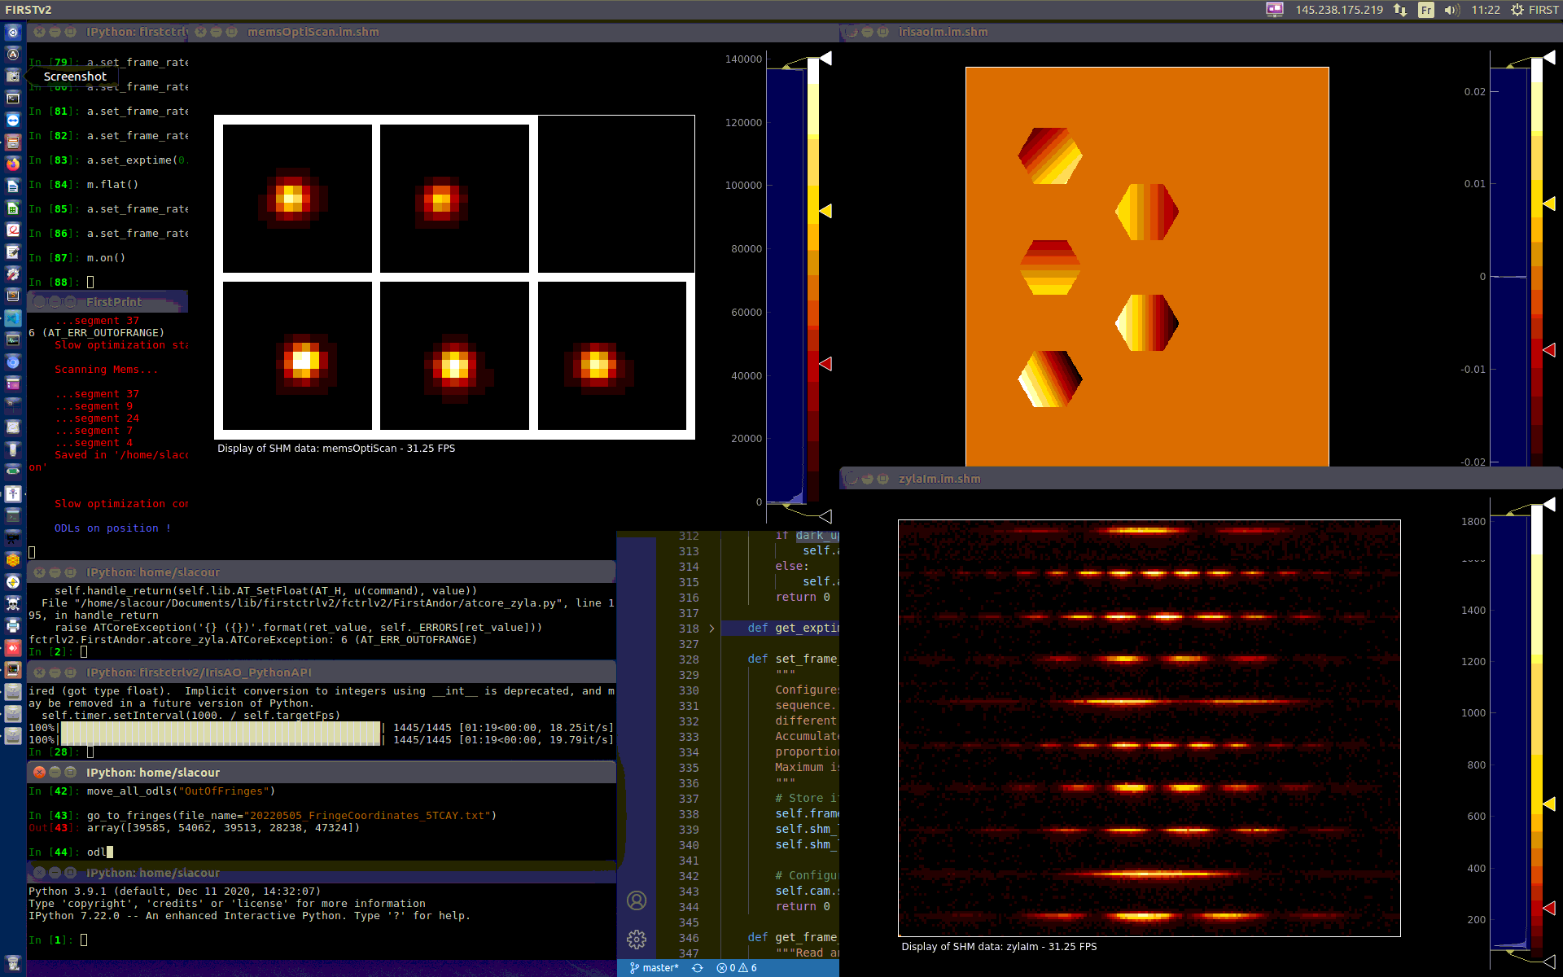
\includegraphics[width=\figwidth]{Figure_Chap2/20220505_5TC_AY_InjectionOpti_Fringes_Meudon.png}
    \caption[Capture d'écran de l'ordinateur de contrôle de FIRSTv2 montrant une optimisation de l'injection et les interférogrammes.]{Capture d'écran de l'ordinateur de contrôle de FIRSTv2. En haut à gauche : les cinq cartes de transmission des fibres, après le quadrillage par les segments du MEMS sur un intervalle de tip-tilt de $\pm 2 \,$mrad avec un pas $0.25 \,$mrad. En haut à droite : la carte de phase du MEMS avec les cinq segments en question en position d'injection du flux maximale. En bas à droite : l'image en direct de la caméra avec les dix sorties de la puce Y, présentant des franges, illuminées par une source SLED à $650 \,$nm.}
    \label{fig:OptiInj}
\end{figure}


%%%%%%%%%%%%%%%%
\subsection{Les lignes à retard}

%%%%%%%%
\subsubsection{Concept}

Les lignes à retard (ou \acrfull{ODL}) sont cruciales pour compenser les longueurs différentes entre les fibres optiques utilisées. En effet, il est nécessaire que la différence de marche (ou \acrfull{OPD}) entre toutes les fibres optiques soit nulle pour obtenir la frange centrale des interférogrammes imagés sur la caméra. La figure~\ref{fig:ODLScheme} montre le schéma de principe d'une ligne à retard, fabriquée par \textit{Oz Optics}. Le faisceau d'une fibre d'entrée, en haut à gauche, est collimaté par une lentille (nommé \textit{lenses} sur le schéma) sur un prisme utilisé en réflexion totale (équivalent à $2$ miroirs), à droite. Ce prisme induit un aller-retour au faisceau qui est focalisé par une autre lentille dans une fibre de sortie (qui est ensuite branché à une fibre d'entrée de la puce photonique), en bas à gauche du schéma. Le prisme est monté sur un moteur contrôlable en position depuis le logiciel de contrôle du banc, sur un intervalle de $25 \,$mm, ce qui résulte en une distance parcourue de $50 \,$mm par le faisceau. Cet intervalle est subdivisé en $100\,000$ pas de $500 \,$nm.

\begin{figure}[ht!]
    \centering
    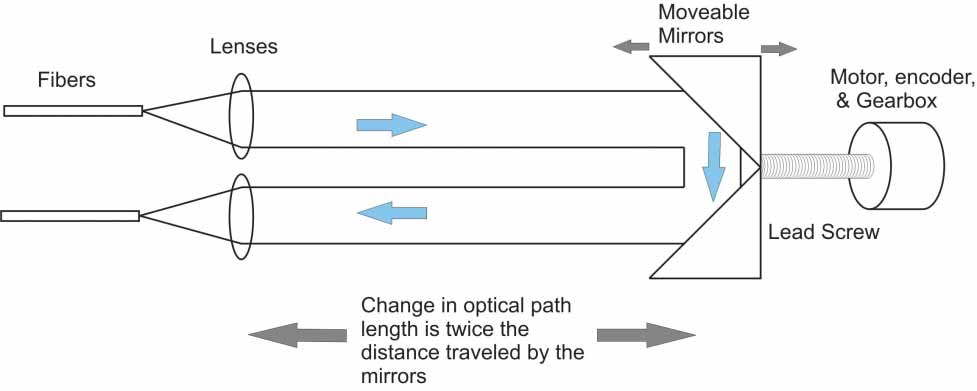
\includegraphics[width=\figwidth]{Figure_Chap2/ODL_Scheme.png}
    \caption[Schéma de fonctionnement d'une ligne à retard.]{Schéma de fonctionnement d'une ligne à retard. Le faisceau est injecté par une fibre en haut à gauche, est collimaté par une lentille (nommé \textit{lenses}) avant d'être réfléchis deux fois par un prisme, à droite, pour faire demi-tour vers la fibre de sortie en bas à gauche. Le prisme est monté sur un moteur permettant de contrôler sa position sur un intervalle de $50\,$mm avec un pas de $500 \,$nm. Crédit : \textit{Oz Optics}.}
    \label{fig:ODLScheme}
\end{figure}


%%%%%%%%
\subsubsection{Transmission}
\label{sec:OdlThroughput}

Au cours de ma thèse, on s'est rendu compte que les \ac{ODL}s transmettaient peu de flux lumineux. En effet, lors de l'intégration anticipée de cinq nouvelles \ac{ODL}s sur l'instrument \ac{FIRSTv1}, la différence d'intensité lumineuse mesurée sur la caméra a été flagrante. Les transmissions les plus basses de celles-ci ont été mesurées à $20 - 30 \%$ alors que la spécification constructeur était une perte de $1,2\,$dB maximum à $650 \,$nm, correspondant à une valeur de transmission de $75\%$. Avec Elsa Huby et Manon Lallement, on a mesuré des transmissions entre $30\%$ et $80\%$ à $675 \,$nm. La figure~\ref{fig:ODLThroughput} présente les mesures de transmission des \ac{ODL}s (exceptée l'\ac{ODL} $\#2$) en fonction de la longueur d'onde à l'aide d'un spectrographe fibré. Pour chaque \ac{ODL}, ces mesures sont effectuées en injectant la lumière soit dans la fibre d'entrée (\textit{In Out}) soit dans la fibre de sortie (\textit{Out In}) pour évaluer si on peut obtenir de meilleures transmissions en injectant dans le sens opposé. On remarque premièrement que la transmission ne dépend pas significativement du sens de propagation dans l'\ac{ODL}. Deuxièmement, la transmission est chromatique (à cause des lentilles) et atteint un maximum vers $675 \,$nm. Les transmissions les plus basses sont celles des lignes à retard $\#3$ et $\#4$. De plus, nous ne disposons pas de la mesure de transmission de l'\ac{ODL} $\#2$ car elle avait été expédiée au fabriquant pour investigation sur la très mauvaise transmission (mesurée à $12\%$ au laboratoire). Il a été diagnostiqué que les fibres d'entrée et de sortie étaient la cause de la faible transmission car elles ont été trouvées endommagées.

\begin{figure}[ht!]
    \centering
    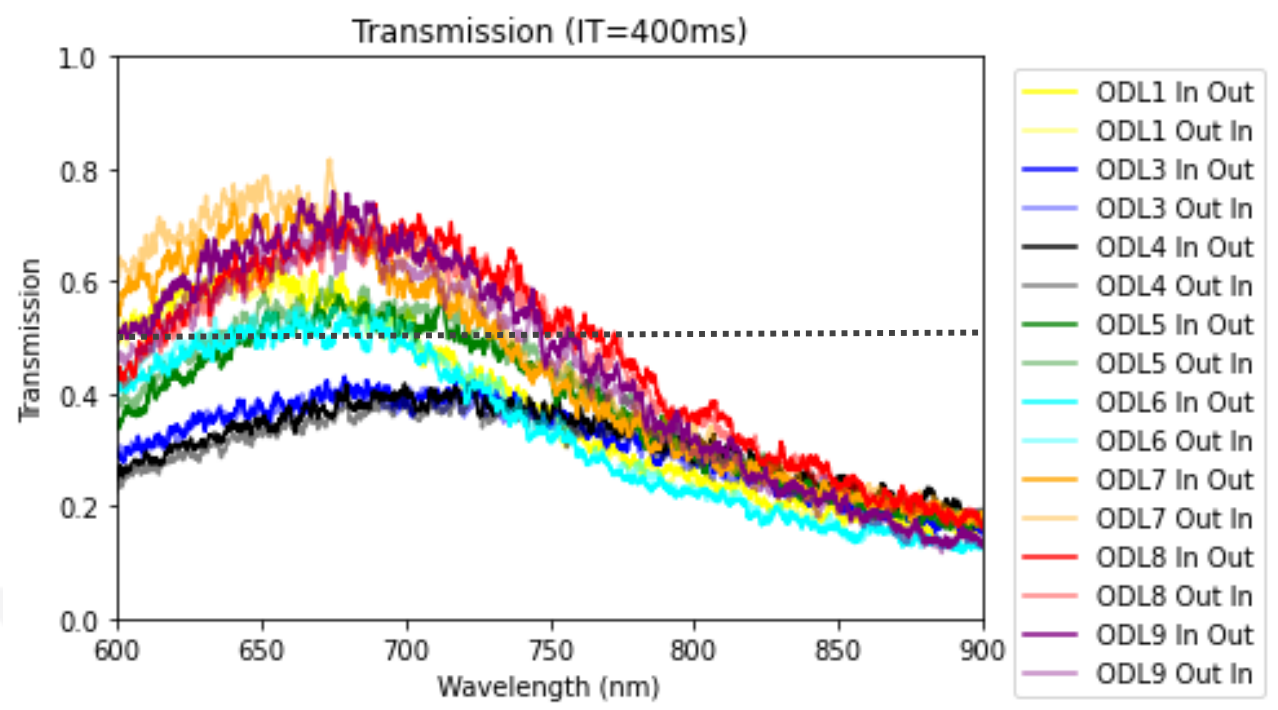
\includegraphics[width=\figwidth]{Figure_Chap2/ODL_Throughput_VS_Wavelength.png}
    \caption[Transmissions des ODLs du banc de test FIRSTv2 mesurées en fonction de la longueur d'onde.]{Transmissions des ODLs du banc de test FIRSTv2 mesurées en fonction de la longueur d'onde à l'aide d'un spectrographe fibré. Pour chaque ODL, la transmission est mesurée en injectant la lumière dans la fibre d'entrée (courbe en couleur foncée) et en injectant la lumière dans la fibre de sortie (en couleur claire). Crédit : Elsa Huby et Manon Lallement.}
    \label{fig:ODLThroughput}
\end{figure}

Nous avons finalement décidé d'en ouvrir une afin d'investiguer par nous-même la cause du problème. La figure~\ref{fig:ODLOpened} présente une photographie de l'intérieur de l'\ac{ODL} $\#1$ après son ouverture au laboratoire. On peut y voir les deux fibres d'entrée (à gauche) et de sortie (à droite). Un laser rouge est injecté dans la fibre d'entrée afin de voir comment se propage le faisceau à travers le système et on peut voir la diffusion d'une partie de la lumière à travers la lentille de collimation et à travers la colle qui la maintient. Ce pourrait être à ce niveau là que la transmission est en grande partie dégradée. Enfin, on aperçoit le prisme collé sur une pièce noire vissée sur la monture motorisée, en bas de l'image et qui réfléchit le faisceau lumineux.

\begin{figure}[ht!]
    \centering
    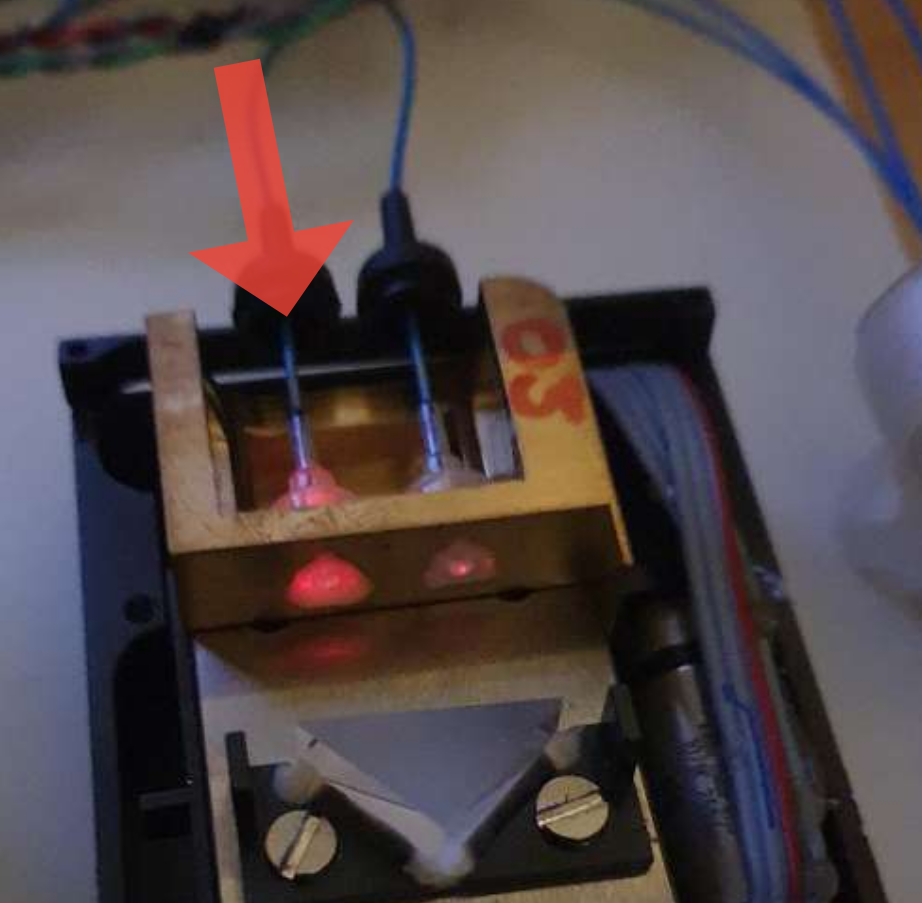
\includegraphics[width=0.6\textwidth]{Figure_Chap2/ODL_Inside_LightInjected_02.png}
    \caption[Photographie d'une ODL ouverte.]{Photographie de l'ODL $\#1$ ouverte. En haut, sont les fibres d'entrée (à gauche) et de sortie (à droite). La lumière d'un laser rouge est injectée dans la fibre d'entrée. Puis plus bas, on voit les lentilles de collimation des faisceaux ainsi que la colle qui les maintient. Le prisme qui réfléchit le faisceau est en bas. Crédit : Elsa Huby et Manon Lallement.}
    \label{fig:ODLOpened}
\end{figure}


%%%%%%%%
\subsubsection{La recherche des franges}

J'ai programmé une procédure de recherche de franges dans le logiciel de contrôle du banc consistant à balayer les lignes à retard sur leur intervalle de position. Plus précisément, une des lignes à retard est laissée immobile à la position la plus basse pendant que toutes les autres \ac{ODL}s sont commandées en translation. Pendant que les \ac{ODL}s se déplacent, la variation de flux est inspectée sur les quatre sorties correspondant aux quatre bases formées par le faisceau passant par l'\ac{ODL} immobile et les quatre autres faisceaux des \ac{ODL}s en mouvement. Dès que les franges sont détectées sur une base, l'\ac{ODL} correspondante est arrêtée et sa position est enregistrée. Si les franges sur les quatre bases sont trouvées, les franges sur toutes les autres bases le sont aussi, nécessairement. Si à la fin du balayage des quatre \ac{ODL}s les franges de toutes les bases ne sont pas trouvées, la ligne à retard restée immobile est déplacée en bout de course (à la position $100\,000$) et le balayage recommence. A la fin de la procédure, lorsque les franges de toutes les bases sont trouvées, on affine les positions des \ac{ODL}s à la main, en regardant l'image en temps réel de la caméra afin de trouver la frange centrale avant de les enregistrer dans un fichier local à l'ordinateur de contrôle. Dans le cas où les franges ne sont pas trouvées sur toutes les bases, cela signifie que la différence de longueur entre les fibres excède $5 \,$cm. Il y a alors la possibilité d'utiliser d'autres \ac{ODL}s dont la longueur de fibre est différente (nous disposons en tout de neuf lignes à retard car à terme il est question de recombiner neuf sous-pupilles comme sur \ac{FIRSTv1}). Les fibres internes aux lignes à retard ont une longueur égale à $\sim 1 \,$m et les incertitudes sur ces longueurs ainsi que celles sur les longueurs des fibres du toron et du V-Groove d'entrée de la puce impliquent qu'il n'est parfois pas possible d'égaliser les longueurs de toutes les fibres du banc.


%%%%%%%%
\subsubsection{Discussions}

Étant donné que la transmission est le point critique à améliorer pour augmenter la sensibilité de l'instrument, il est essentiel d'identifier les sources de pertes de transmission. L'étude présentée dans la partie~\ref{sec:OdlThroughput}, nous montre que les lignes à retard présentent une perte de transmission considérable et de nouvelles solutions sont envisagées afin de les retirer de l'instrument.

% Alternative 1 : fibres de compensation
La solution qui sera probablement implémentée prochainement est de remplacer les lignes à retard par des fibres de compensation. C'est la solution choisie sur \ac{FIRSTv1} et présentée dans la thèse d'Elsa Huby \citep{huby2013these}. Cela demanderait de mesurer les longueurs des fibres du toron et des fibres d'entrée de la puce afin de les égaliser. La longueur de cohérence étant ici égale à $\text{l}_\text{c} = 2,21 \,$mm à $650 \,$nm, pour une résolution spectrale égale à $3\,400$ (voir la section~\ref{sec:InstruSpectro}), la précision sur l'égalisation des longueurs doit donc être de $1,1 \,$mm. C'est une charge conséquente de travail en plus mais qui serait justifiée par le gain conséquent en transmission.

% Alternative 2 : puce photonique 3D
Une autre solution serait de changer tout le système d'injection et deux concept sont envisagés. Premièrement, la matrice de micro-lentille pourrait être placée directement entre le \ac{MEMS} et la puce d'optique intégrée afin d'injecter les faisceaux des sous-pupilles directement dans cette dernière. Les guides d'ondes de la puce seraient alors gravées dans les trois dimensions de la puce (et non dans un plan comme c'est le cas sur les puces utilisées lors de cette thèse) afin de les placer devant les sous-pupilles choisies pour la recombinaison interférométrique et de les placer sur une ligne en sortie de la puce. En plus d'avoir l'avantage de se passer du toron de fibres et des lignes à retard, cela permet aussi de recombiner par paire tous les faisceaux sans aucun croisement des guides d'ondes, ce qui constitue une source de \textit{cross-talk} et de perte de transmission (voir plus de détails dans la section~\ref{sec:ChipCharacterization}). Ce concept est déjà exploité dans l'instrument \ac{GLINT} \citep{martinod2021} et a été développé à l'\ac{IPAG} (voir son schéma de principe sur la figure~\ref{fig:Chip5T3D}) pour le projet \ac{FIRST} et testé sur le banc de test de \ac{FIRSTv2} \citep{martin2022a}.

\begin{figure}[ht!]
    \centering
    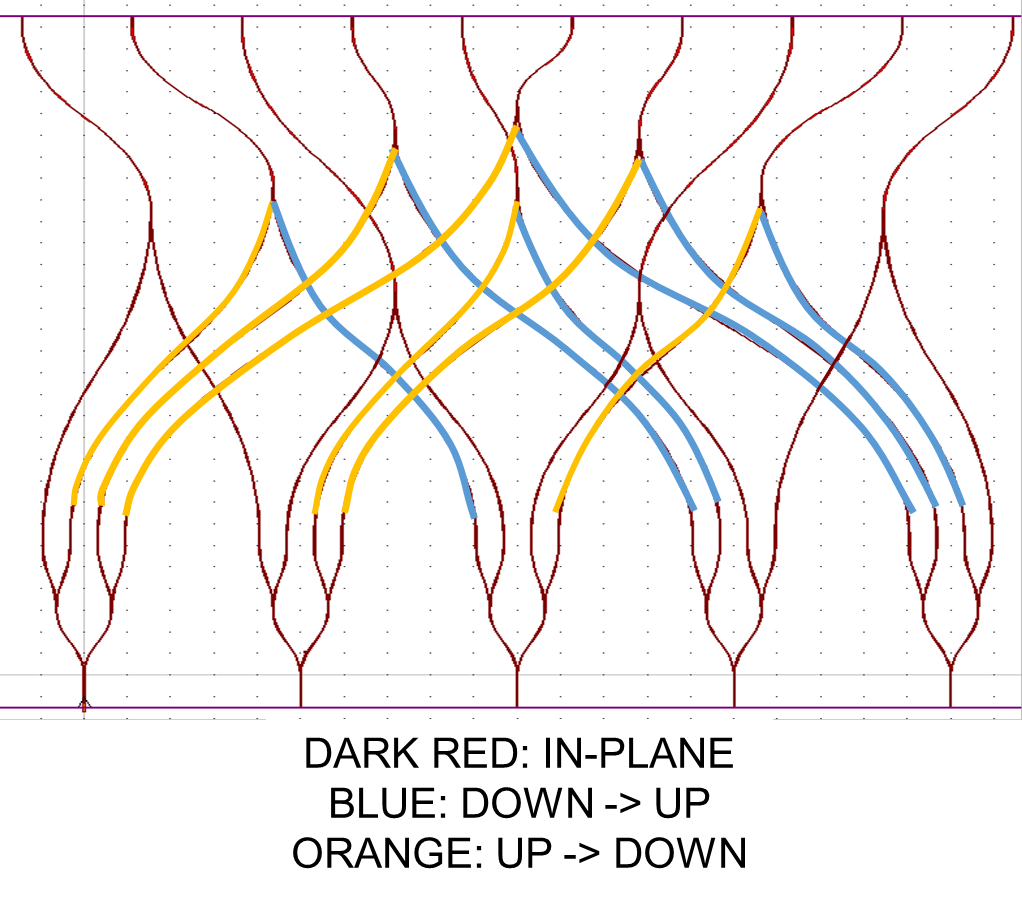
\includegraphics[width=0.8\textwidth]{Figure_Chap1/Martin2022_FIRST573D_Figure1.png}
    \caption[Schéma de principe du concept de puce photonique 3D.]{Schéma de principe du concept de puce photonique 3D. Les entrées sont en bas et les sorties en haut. Trois types de guides d'onde sont représentés : dans le plan (en rouge), qui monte puis descend (en orange) et qui descend puis monte (en bleu). Crédit : Guillermo Martin.}
    \label{fig:Chip5T3D}
\end{figure}

% Alternative 3 : photonic lantern
Deuxièmement, on envisage d'intégrer une lanterne photonique \citep{leonsaval2005} à la place des puces actuelles. Le principe de cette technologie est de convertir un faisceau injecté dans une fibre optique multi-mode en plusieurs faisceaux dans des fibres optiques mono-modes. En mesurant l'intensité en sortie des fibres optiques mono-modes, il est possible de remonter à la phase du front d'onde d'entrée. La relation entre les sorties et l'entrée d'une telle puce est non-linéaire et \cite{norris2020a} propose d'utiliser un réseau de neurones pour remonter aux aberrations du front d'onde d'entrée et utilise ce système comme senseur de front-d'onde pour l'optique adaptative. Des discussions ont lieu avec Barnaby Norris afin de dimensionner un tel composant travaillant dans le visible pour son application future dans le projet \ac{FIRST}. Cela permettrait de se passer de la matrice de micro-lentille, du toron de fibres et des lignes à retard (seule une lentille suffirait pour injecter le faisceau dans la fibre d'entrée de la lanterne photonique) et optimiserait l'utilisation de tout le flux lumineux injecté dans l'instrument puisque toute la pupille est injectée dans le composant.


%%%%%%%%%%%%%%%%
\subsection{Les composants d'optique intégrée}
\label{sec:PhotonicChip}
% Low bend radius ---> high refractive index difference
% IMEC material of Si3N4 core with SiO2 cladding but the waveguide has to be very small and difficult to use them in the visible
% The material thickness is such that at a 670nm wavelength the mode is well confined in the core. As a result the bend radius is small, at 20 microns.

% High bend radius ---> low refractive index difference
% Teem material of SiN core and SiO2 cladding
% LioniX is same material but deposited differently

% The bend radius decreases with the thickness of the waveguide

% A small bend radius allows us to use adiabatic bends which will further decrease the loss but that is the next level. An adiabatic bend (if you don't know) just means that we don't just use one bend radius but start high at the start of the bend and decrease until a bend radius minima at the middle before increasing it again. This increases the total length of the bend but removes any loss between the straight waveguides and the bend.


%%%%%%%%
\subsubsection{Concept}
\label{sec:ChipConcept}

Les puces d'optique intégrée (photonique) sont conçues à l'\ac{IPAG} et testées sur le banc \ac{FIRSTv2} \citep{martin2020, martin2022b, lallement2022} et sont fabriquées par \textit{Teem Photonics}\footnote{\url{https://www.teemphotonics.com}}. Elles consistent en un bloc de verre de quelques centimètres (voir la photographie de la puce $Y$ sur la figure~\ref{fig:ChipYPhoto}), utilisant la technologie IoNext par échange des ions $\text{K}_+ : \text{Na}_+$, dans lequel des guides d'onde sont fabriqués par des techniques classiques de photolithographie. Les fibres d'entrée et de sortie sont celles de V-Grooves collés au bloc de verre par le fabriquant et sont branchées sur les \ac{ODL}s et sur un autre V-Groove, respectivement. Cette technologie est très utilisée dans le domaine des télécommunications optiques dans l'infrarouge proche alors que les puces développées pour le projet \ac{FIRSTv2} ont été optimisées pour être transmissives dans la bande spectrales $\sim 600 - 800 \,$nm.

\begin{figure}[ht!]
    \centering
    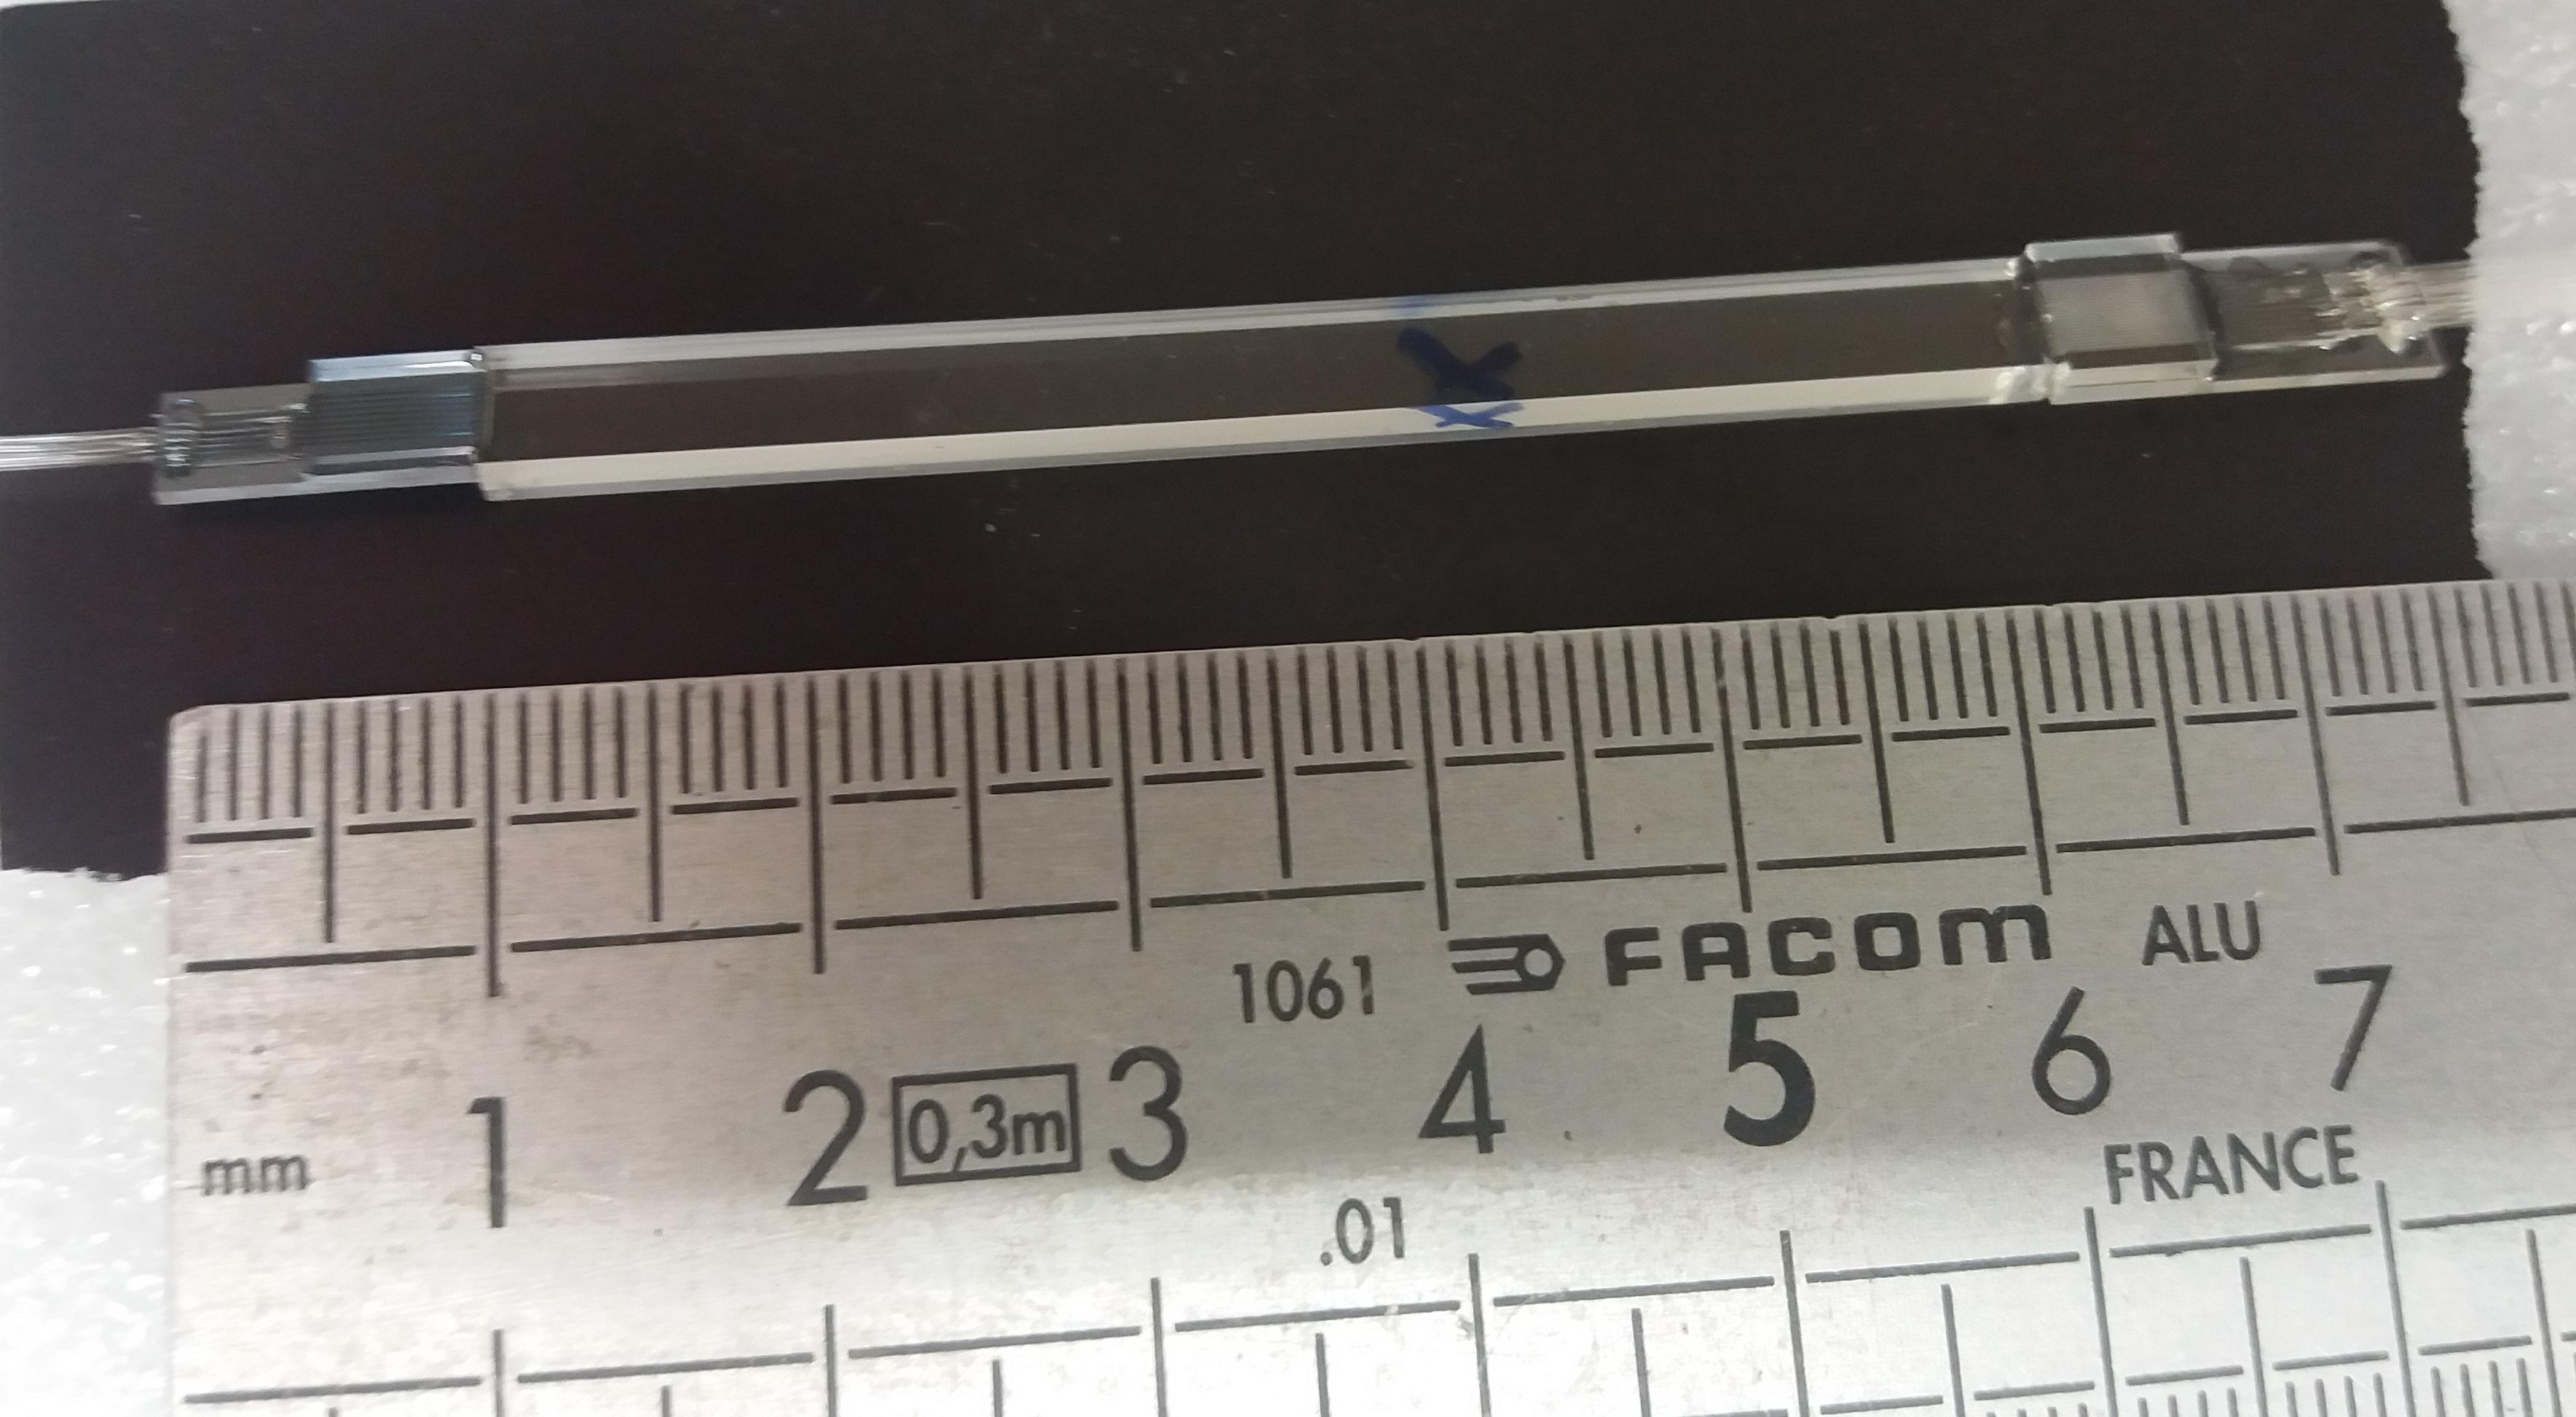
\includegraphics[width=\figwidth]{Figure_Chap2/PhotonicChip_5T_YComb_Meudon_04_crop.jpg}
    \caption[Photographie de la puce $Y$ testée sur le banc de test de \ac{FIRSTv2} à Meudon.]{Photographie de la puce $Y$ testée sur le banc de test de \ac{FIRSTv2} à Meudon.}
    \label{fig:ChipYPhoto}
\end{figure}

Durant ma thèse, j'ai testé \citep{barjot2020} sur \ac{FIRSTv2} deux technologies de puces photoniques nommées $X$ et $Y$, dont les schémas de principe sont montrés sur la figure~\ref{fig:ChipSchemes}, à gauche et à droite, respectivement. Les deux puces ont cinq guides d'onde en entrée (à gauche des schémas) qui sont chacun divisé en quatre (zone nommée \textit{splitting}). Chaque faisceau est recombiné par paires avec les quatre autres (zone nommée \textit{recombination}). Les faisceaux des cinq sous-pupilles du banc sont injectés dans ces entrées. La puce $X$ contient des coupleurs dit directionnels qui recombinent les faisceaux par couplage évanescent : il y a deux guides d'entrée et deux guides de sortie. La puce $Y$ recombine les faisceaux à l'aide de coupleurs $Y$ qui fusionne deux guides en un seul : il y a deux guides d'entrée et un guide de sortie. En sortie, dix bases ($5 \times 4 / 2$) sont ainsi formées. Dans le cas de la puce $X$ on dispose de deux sorties par base, du fait de la technique de couplage directionnel. On mesure alors le double de flux avec cette puce par rapport à la puce $Y$. Pour chaque base, les franges d'interférences obtenues sur les deux sorties ont un déphasage théorique de $\pi \,$rad.

\begin{figure}[ht!]
    \centering
    \begin{subfigure}{0.5\textwidth}
        \centering
        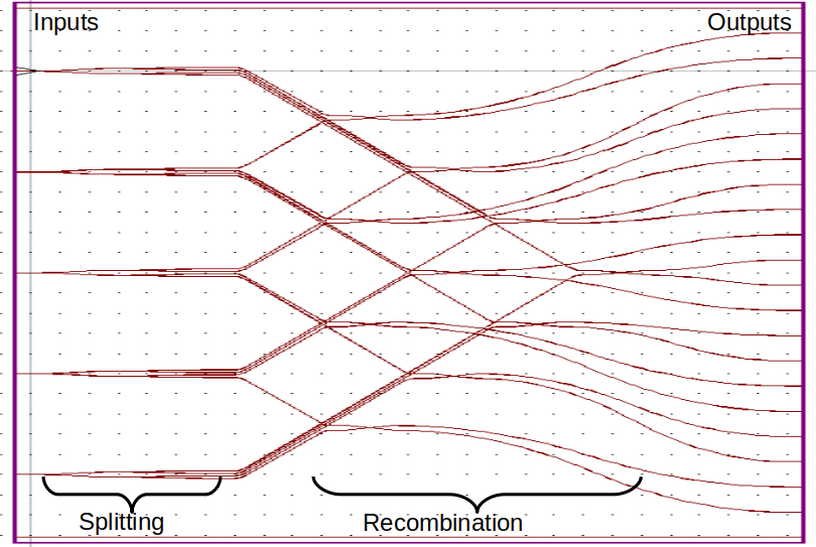
\includegraphics[width=\textwidth]{Figure_Chap2/5TC_X_ChipScheme_rot_l_01.png}
    \end{subfigure}%
    \begin{subfigure}{0.5\textwidth}
        \centering
        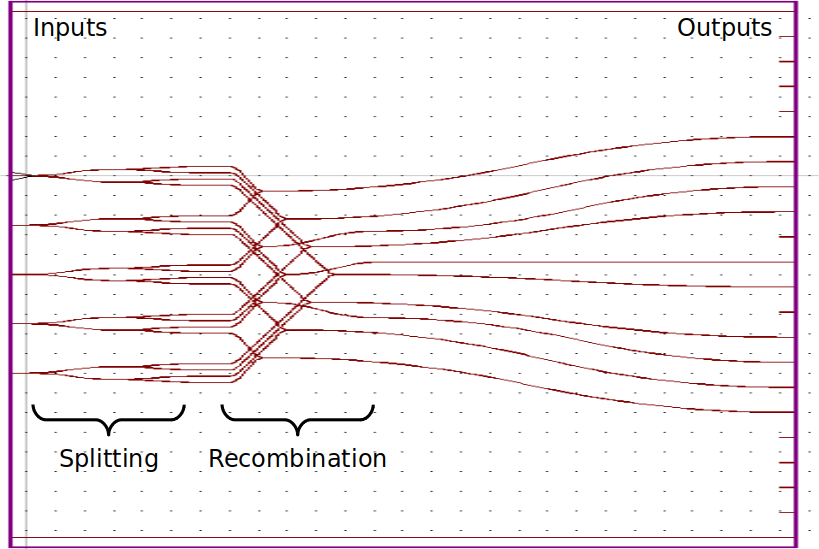
\includegraphics[width=\textwidth]{Figure_Chap2/5TC_Y_ChipScheme_rot_l_02.png}
    \end{subfigure}
    \caption[Schémas de principe des puces photoniques $X$ et $Y$.]{Schémas de principe des puces photoniques $X$ à gauche et $Y$ à droite. Les lignes représentent les guides d'onde dont les entrées sont à gauche et les sorties sont à droite. De la gauche vers la droite, les deux puces ont cinq guides d'onde en entrée qui sont d'abord divisés en quatre (zone nommée \textit{splitting}), afin d'être (plus loin) recombinés par paires avec les quatre autres (zone nommée \textit{recombination}). La puce $X$ a deux fois plus de fibres de sortie que la puce $Y$ du fait de la technique de couplage directionnel. Crédit : Guillermo Martin.}
    \label{fig:ChipSchemes}
\end{figure}


%%%%%%%%
\subsubsection{Caractérisation}
\label{sec:ChipCharacterization}

Pour caractériser les deux puces photoniques, j'ai utilisé une source large bande halogène de la gamme \textit{HL-2000-FHSA-HP}, fabriquée par \textit{Ocean Insight}\footnote{\url{https://www.oceaninsight.com/}}, lumineuse dans la gamme spectrale $360 - 2400 \,$nm. Cette caractérisation est publiée dans \cite{barjot2020} (voir la section~\ref{sec:SPIEproceeding}) et je la rappelle ici. Trois études sont conduites sur les deux puces :

\begin{enumerate}
    \item le cross-talk, qui caractérise la quantité de fuite du signal entre les différents guides d'onde
    \item la transmission
    \item le contraste interférométrique
\end{enumerate}


% Caractérisation du cross-talk
\threesubsection{\textit{Cross-talk}}

Pour estimer le \textit{cross-talk}, cinq images de la caméra sont acquises successivement en illuminant les cinq entrées des puces photoniques, sans passer par le reste du banc de test en amont. La figure~\ref{fig:ChipCrossTalk} présente les cinq histogrammes correspondant à l'intensité lumineuse mesurée sur toutes les sorties de la puce $X$ en haut et de la puce $Y$ en bas. On s'attend à mesurer une intensité lumineuse sur $4$ ou $8$ sorties (représentées par les barres de couleur bleue) pour les puces $Y$ et $X$, respectivement et une intensité nulle sur les sorties restantes (représentées par les barres de couleur rouge). Ainsi, le flux mesuré sur les sorties en rouge est l'estimation du \textit{cross-talk}. On estime ainsi que le \textit{cross-talk} est en moyenne égal à $\sim 1\%$ pour les deux puces et est dans le pire des cas égal à $10 \%$ et à $20 \%$ en moyenne pour la puce $X$ et pour la puce $Y$, respectivement. Notre objectif est d'abaisser ce niveau à moins de $1\%$ (dans le pire des cas) et de nouvelles puces utilisant d'autre technologies et d'autres matériaux sont en cours de développement et de test par l'équipe travaillant à Grenoble, dans ce but.

Le \textit{cross-talk} intervient ici de deux façons différentes. Premièrement, la lumière fuit au niveau des croisements entre les guides et la fuite est d'autant plus importante que l'angle au croisement est petit \citep{labeye2008}. En effet, les niveaux de \textit{cross-talk} les plus élevés sur la figure~\ref{fig:ChipCrossTalk} correspondent aux guides d'onde qui croisent les guides dans lesquels la lumière est injectée. Par exemple, sur le graphique du haut (de la puce $X$), dans l'histogramme du cas où la lumière est injectée dans l'entrée $1$, ce sont les sorties $5$, $6$ et $7$ qui sont concernées par ce phénomène. La difficulté dans la conception des puces réside dans le fait que la courbure des guides d'onde est limitée (la fuite de la lumière en dehors des guides augmente avec la courbure des guides) car ces puces sont basées sur des guides à faible contraste d'indice ($10^{-3} - 10^{-4}$). Cela ne permet donc pas de croiser les guides avec des angles plus grand que $5\degree$, non atteignables avec le faible confinement obtenu (c'est l'ordre de grandeur des angles des croisements utilisés dans les puces testées sur \ac{FIRSTv2}). Il est possible d'utiliser des matériaux différents dans le but de diminuer les rayons de courbure des guides d'onde. Il s'agit pour cela de choisir les matériaux du coeur et de la gaine de sorte que la différence de leurs indices de réfraction soit plus élevée. Les inconvénients de cette solution sont que ces puces sont moins transmissives dans le visible et que les coeurs doivent être plus petits : typiquement de l'ordre de quelques centaines de nanomètres pour des guides avec des contrastes d'indice de $0,1 - 0,5$. Cela augmente la difficulté de couplage entre les modes de petite taille des guides de la puce avec les modes des fibres optiques standard. Deuxièmement, une partie du flux est diffusée dans toute la puce à l'extérieur des guides, au niveau de l'injection de la lumière en entrée de la puce, due aux erreurs de couplage entre les modes d'injection et les modes guidés. Ce phénomène peut se mesurer sur les sorties qui ne sont pas en aval de croisements avec les guides dont la lumière est injectée. Sur les mesures de caractérisation, le niveau de \textit{cross-talk} sur ces sorties est mesuré $10 \times$ inférieur que les autres sorties (en aval de croisement). Par exemple sur le graphique du haut de la figure~\ref{fig:ChipCrossTalk}, lorsque l'entrée $1$ est illuminée, les sorties dont le niveau de \textit{cross-talk} est concerné par ce phénomène sont celles numérotées de $12$ à $20$. De plus, on remarque que ce niveau décroît avec la distance entre la sortie et l'entrée dans laquelle la lumière est injectée. On retrouve cet effet sur tous les histogrammes des deux graphiques.

\begin{figure}[ht!]
    \centering
    \begin{subfigure}{0.9\textwidth}
        \centering
        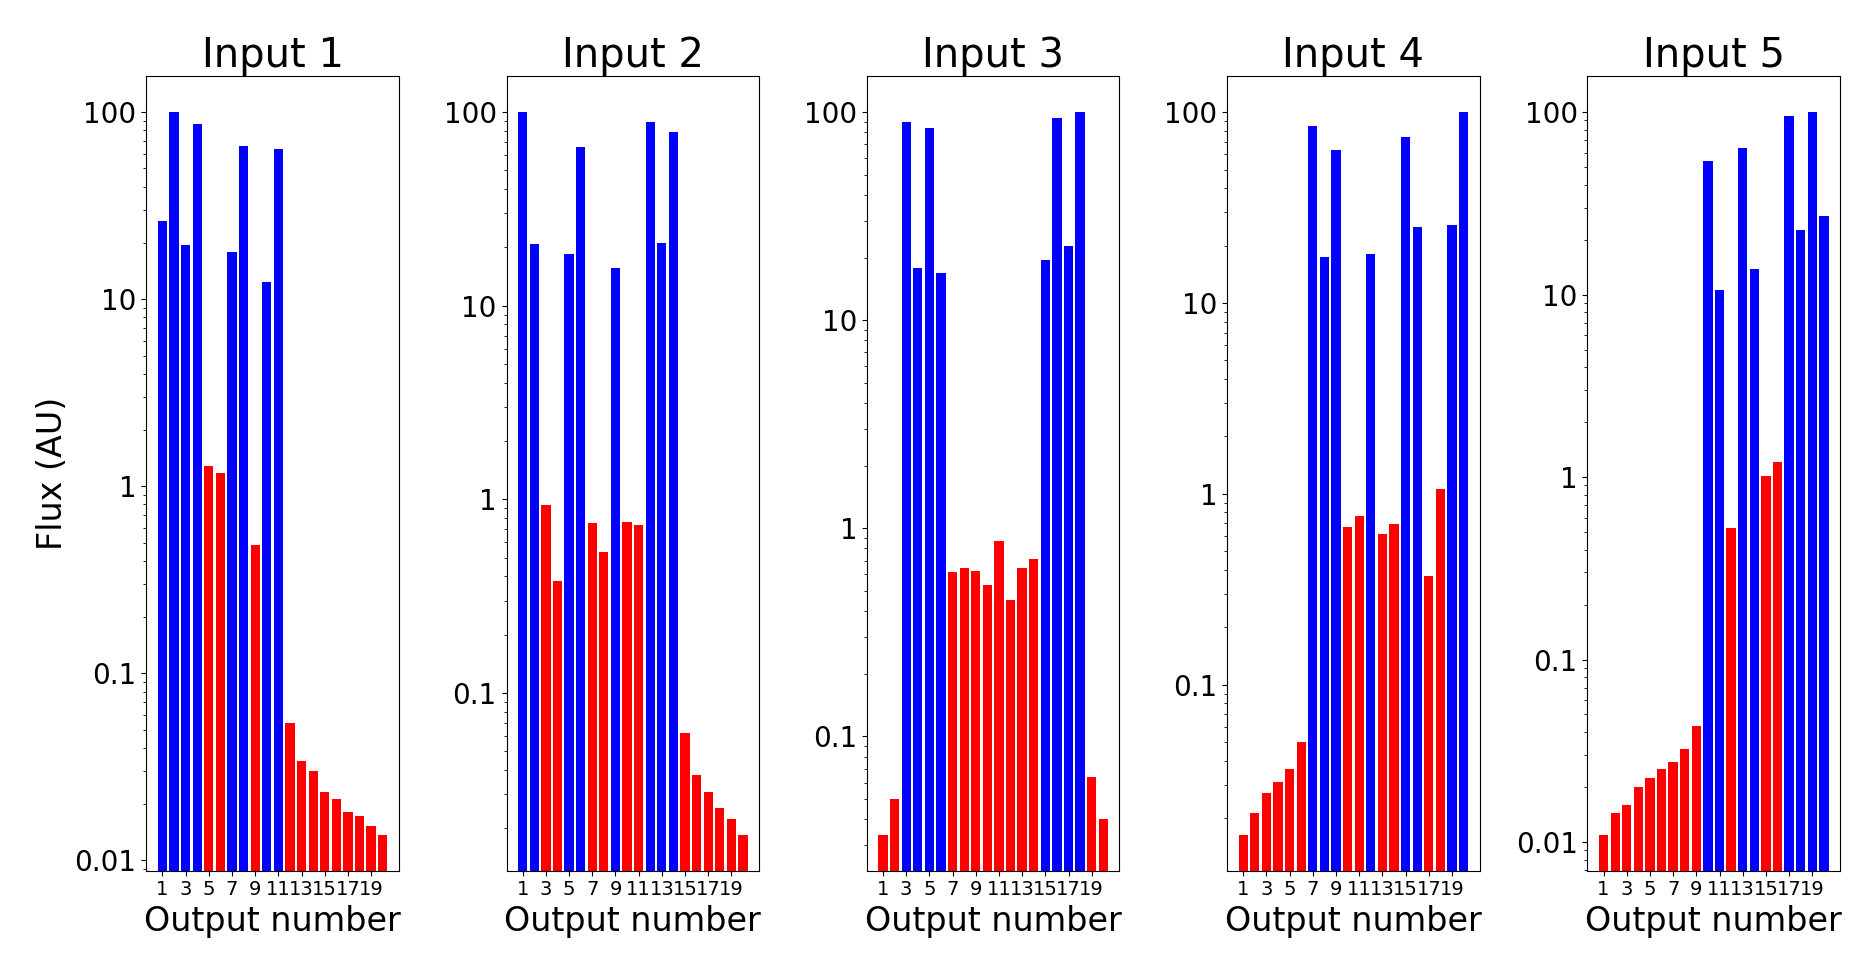
\includegraphics[width=\textwidth]{Figure_Chap2/20201124_5TC_5OutputFluxesLog_OOptics_LaTex.png}
    \end{subfigure}
    \begin{subfigure}{0.9\textwidth}
        \centering
        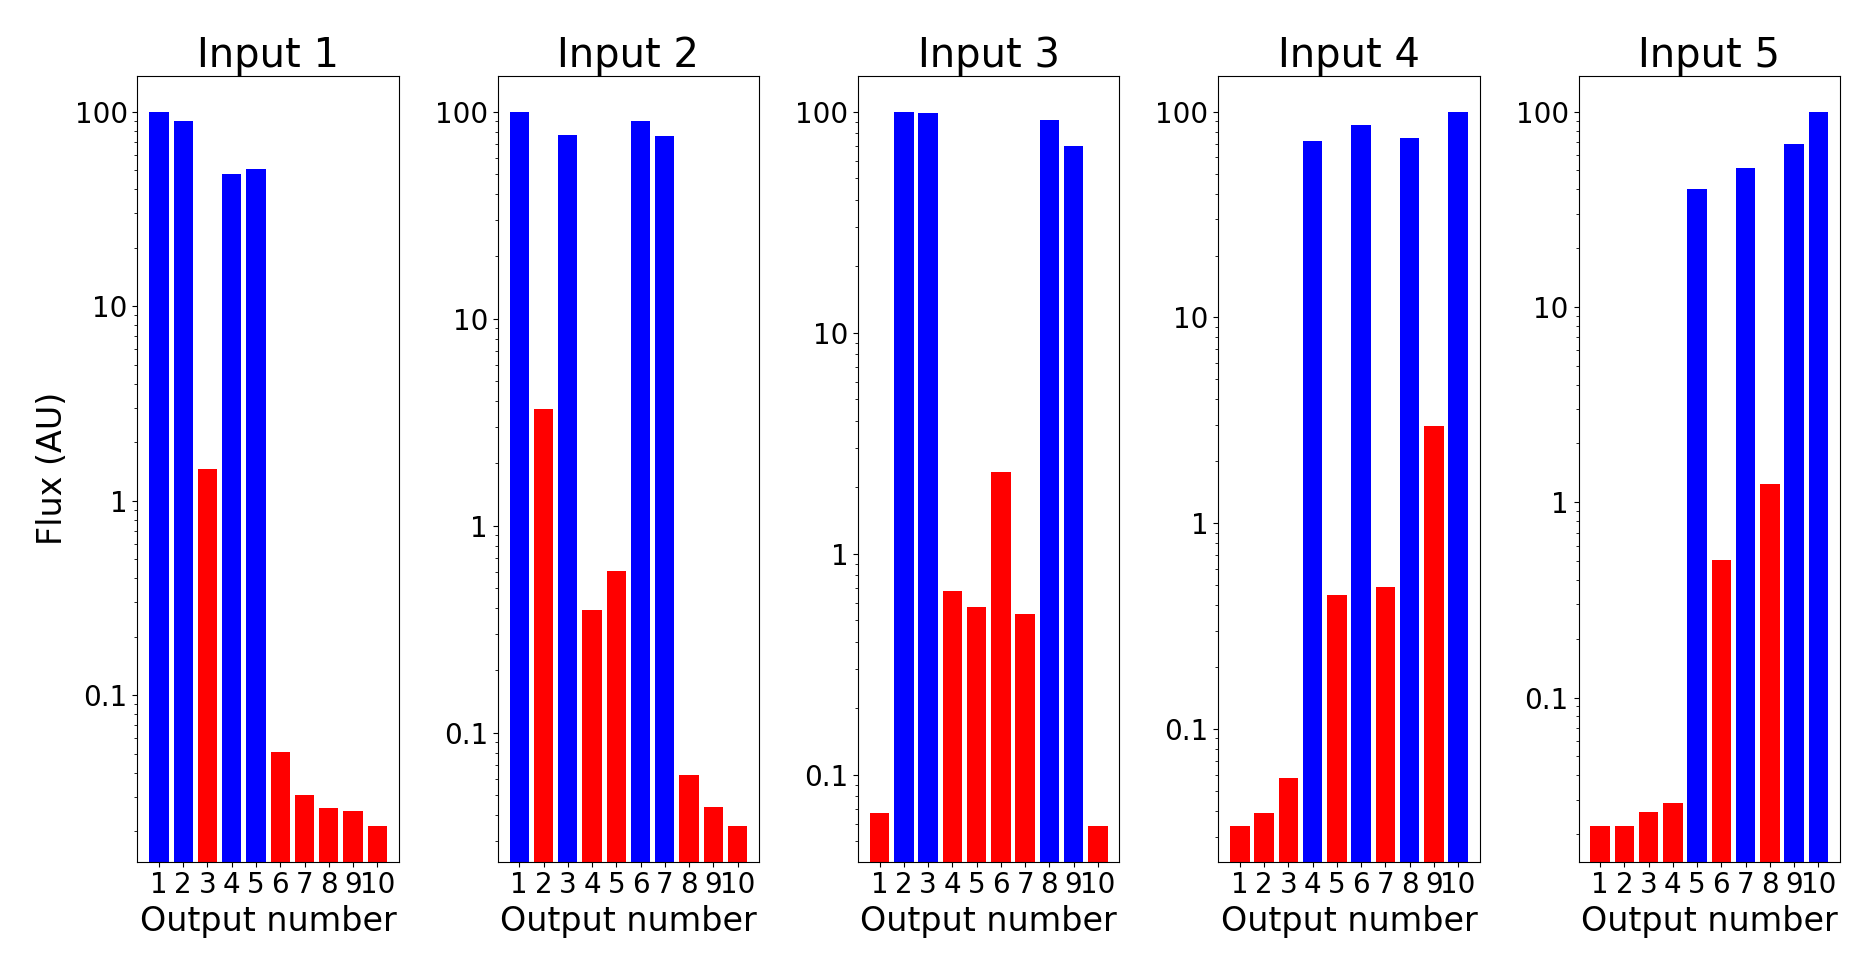
\includegraphics[width=\textwidth]{Figure_Chap2/20201119_5TC_5OutputFluxesLog_OOptics_LaTex.png}
    \end{subfigure}
    \caption[Histogrammes de l'estimation du \textit{cross-talk} des puces photoniques $X$ et $Y$.]{Histogrammes en échelle logarithmique de l'estimation du \textit{cross-talk} des puces photoniques $X$ (en haut) et $Y$ (en bas). La source lumineuse est successivement injectée dans les cinq entrées des puces (nommé \textit{input \#} dans les sous-titres) et l'intensité lumineuse de toutes les sorties est à chaque fois estimée sur l'image de caméra. La mesure de l'intensité lumineuse des sorties illuminées par l'entrée ($4$ et $8$ pour les puces $Y$ et $X$) est représentée par des barres bleues et la mesure de l'intensité lumineuse des sorties non-illuminées par l'entrée ($6$ et $12$ pour les puces $Y$ et $X$) est représentée par des barres rouges sur les histogrammes.}
    \label{fig:ChipCrossTalk}
\end{figure}


% Caractérisation de la transmission
\threesubsection{Transmission}

Le flux total transmis par la puce est calculé par la somme des flux mesurés sur les cinq images acquises pour la caractérisation du \textit{cross-talk}. On note que le flux provenant du \textit{cross-talk} n'a pas été retiré dans la somme du flux total, ainsi les valeurs de transmission présentées ci-après sont surestimées d'environ $5\%$. Ensuite on obtient la transmission par la normalisation de ce flux par le flux mesuré en injectant la lumière juste après la puce, dans une des fibres du V-Groove connecté aux sorties de la puce. La figure~\ref{fig:ChipThroughput} présente les courbes de transmission calculées de cette façon, en fonction de la longueur d'onde, pour la puce $X$ en trait continu et pour la puce $Y$ en pointillés. Dans la bande spectrale $600 - 800 \,$nm, la transmission de la puce $X$ et de la puce $Y$ est mesurée à $\sim 30\%$ et à $\sim 13\%$, respectivement. Ces valeurs de transmission sont bien plus élevées que celles des puces précédentes testées avant ma thèse (moins de $1\%$) et sont mêmes suffisantes pour qu'on puisse intégrer les puces sur \ac{SCExAO} afin de les tester sur des cibles astrophysiques (pour plus de détails voir la section~\ref{sec:FIRSTv2Subaru}). Le facteur $2$ entre les deux transmissions mesurées est attendu, étant donné que le flux injecté dans le coupleur $Y$ est à moitié transmis dans le sortie et à moitié diffusé en dehors des guides. Le couplage directionnel transmet cette moitié diffusée dans le deuxième guide de sortie (voir plus de détails dans la section II-B-6 de \cite{labeye2008}). On pourrait avoir une préférence pour l'utilisation de la puce $X$ sur \ac{FIRSTv2} pour sa meilleure transmission, mais comme on le verra par la suite, elle ne permet pas d'estimation satisfaisante des observables interférométriques et la puce $Y$ se révèle bien meilleure de ce point de vue là.

\begin{figure}[ht!]
    \centering
    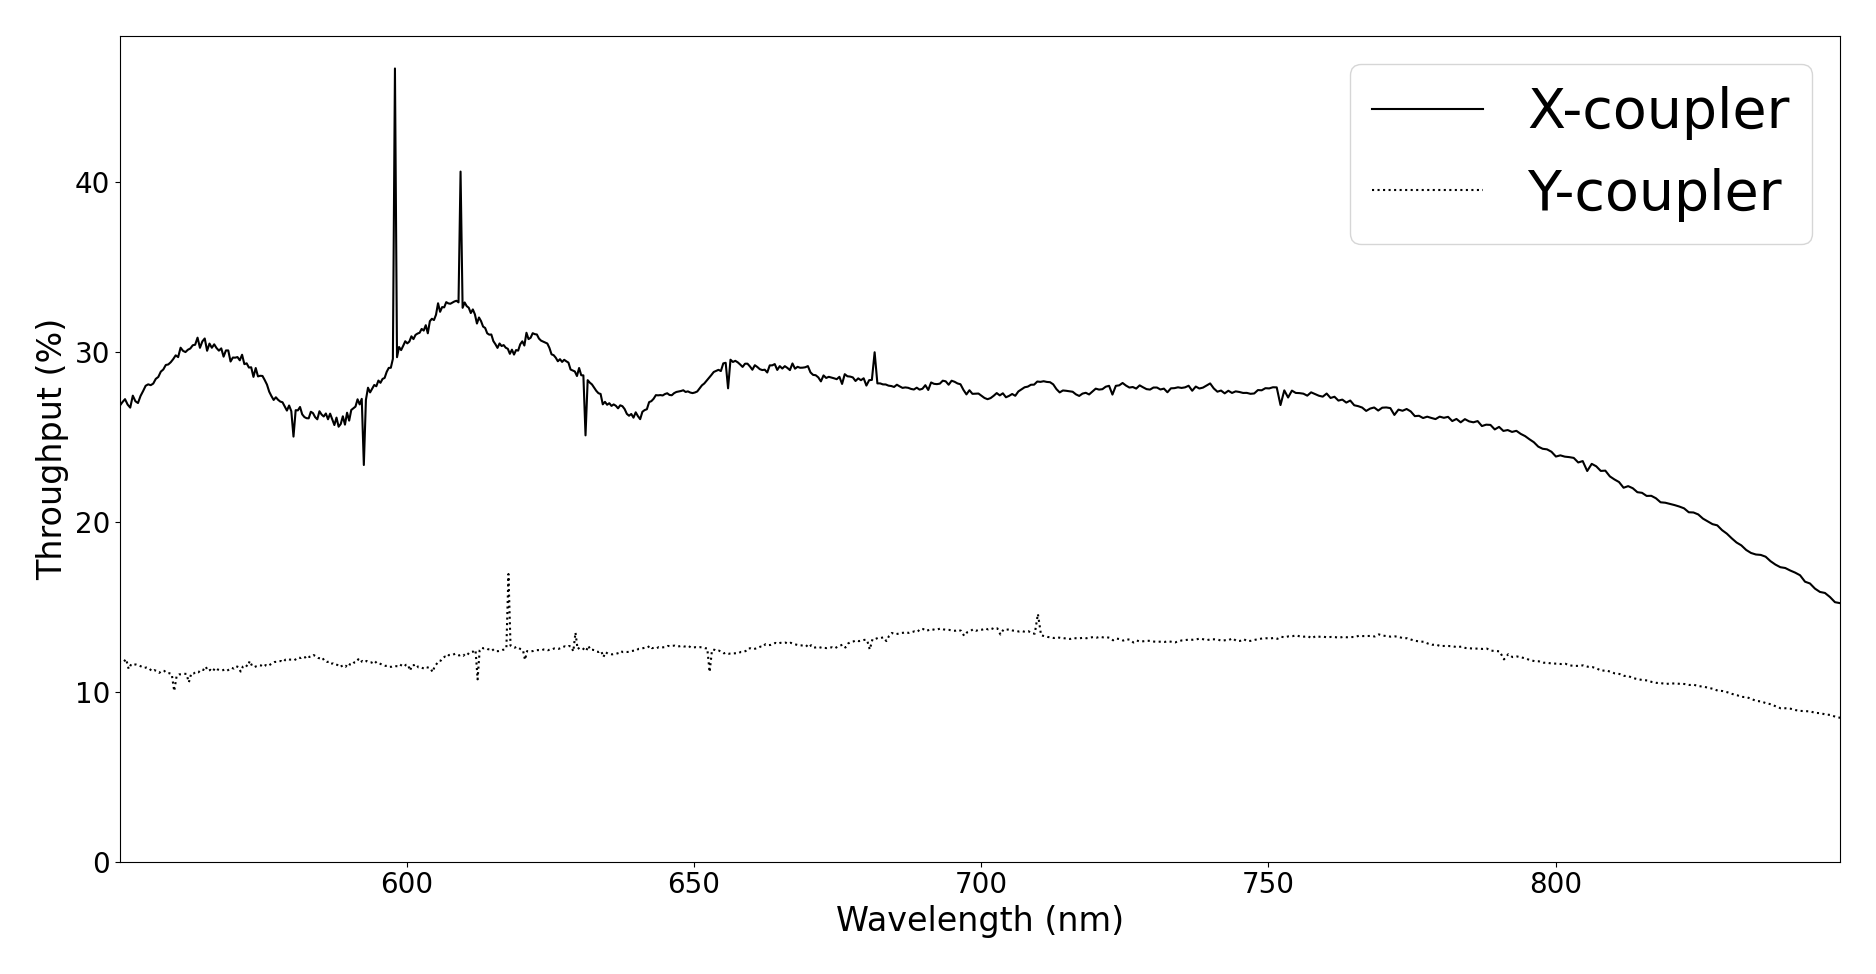
\includegraphics[width=\figwidth]{Figure_Chap2/ThroughputComparison_20201124_20201119_LaTex.png}
    \caption[Transmission spectrale mesurée des puces $X$ et $Y$.]{Transmission spectrale mesurée des puces $X$ en trait continu et $Y$ en pointillés.}
    \label{fig:ChipThroughput}
\end{figure}


% Caractérisation du contraste interférométrique
\threesubsection{Contraste interférométrique}

Cette partie présente la limite haute du contraste interférométrique des bases des deux puces calculé par la différence de flux entre les paires de faisceaux qui interfèrent. Pour une base donnée résultante de la combinaison des faisceaux $n$ et $n'$, je calcule ce contraste C à partir de la mesure de l'intensité des faisceaux $\text{I}_{n}$ et $\text{I}_{n'}$ selon l'équation :

\begin{equation}
    \text{C} = \frac{2 \sqrt{\text{I}_{n} \text{I}_{n'}}}{\text{I}_{n} + \text{I}_{n'}}
\end{equation}

J'utilise les cinq images décrites précédemment pour estimer les valeurs d'intensité de la sortie illuminée par les deux entrées $n$ et $n'$. Autrement dit, les valeurs $\text{I}_{n}$ et $\text{I}_{n'}$ sont obtenues sur la sortie qui est commune aux deux images obtenues en illuminant les entrées $n$ et $n'$ et qui est représentée par une barre bleue sur les histogrammes de la figure~\ref{fig:ChipCrossTalk}. Par exemple, le contraste de la base $5$, formée par les entrées $2$ et $3$, est estimé à partir des intensités mesurées sur la sortie $3$ des histogrammes nommées \textit{Input 2} et \textit{Input 3}, pour la puce $Y$. La figure~\ref{fig:ChipContrast} présente les contrastes interférométriques estimés de cette façon pour toutes les sorties de la puce $X$ (points) et de la puce $Y$ (croix). Les contrastes obtenus avec les puces $X$ et $Y$ sont en moyenne égaux à $0,78$ et $0,994$, respectivement, avec un écart-type de $0,04$ et $0,004$, respectivement. On remarque que le contraste est pratiquement maximal pour la puce $Y$ et est dégradé de $\sim 20\%$ pour la puce $X$ ce qui peut s'expliquer par le fait que les coupleurs directionnels ne sont pas parfaitement équilibrés en transmission de flux sur les deux sorties (visible sur les histogrammes du haut de la figure~\ref{fig:ChipCrossTalk}). Ce contraste correspond à une transmission dans les deux bras de sortie d'environ $80\% / 20\%$ alors que dans l'idéal on s'attend à une transmission de $50\% / 50\%$.

\begin{figure}[ht!]
    \centering
    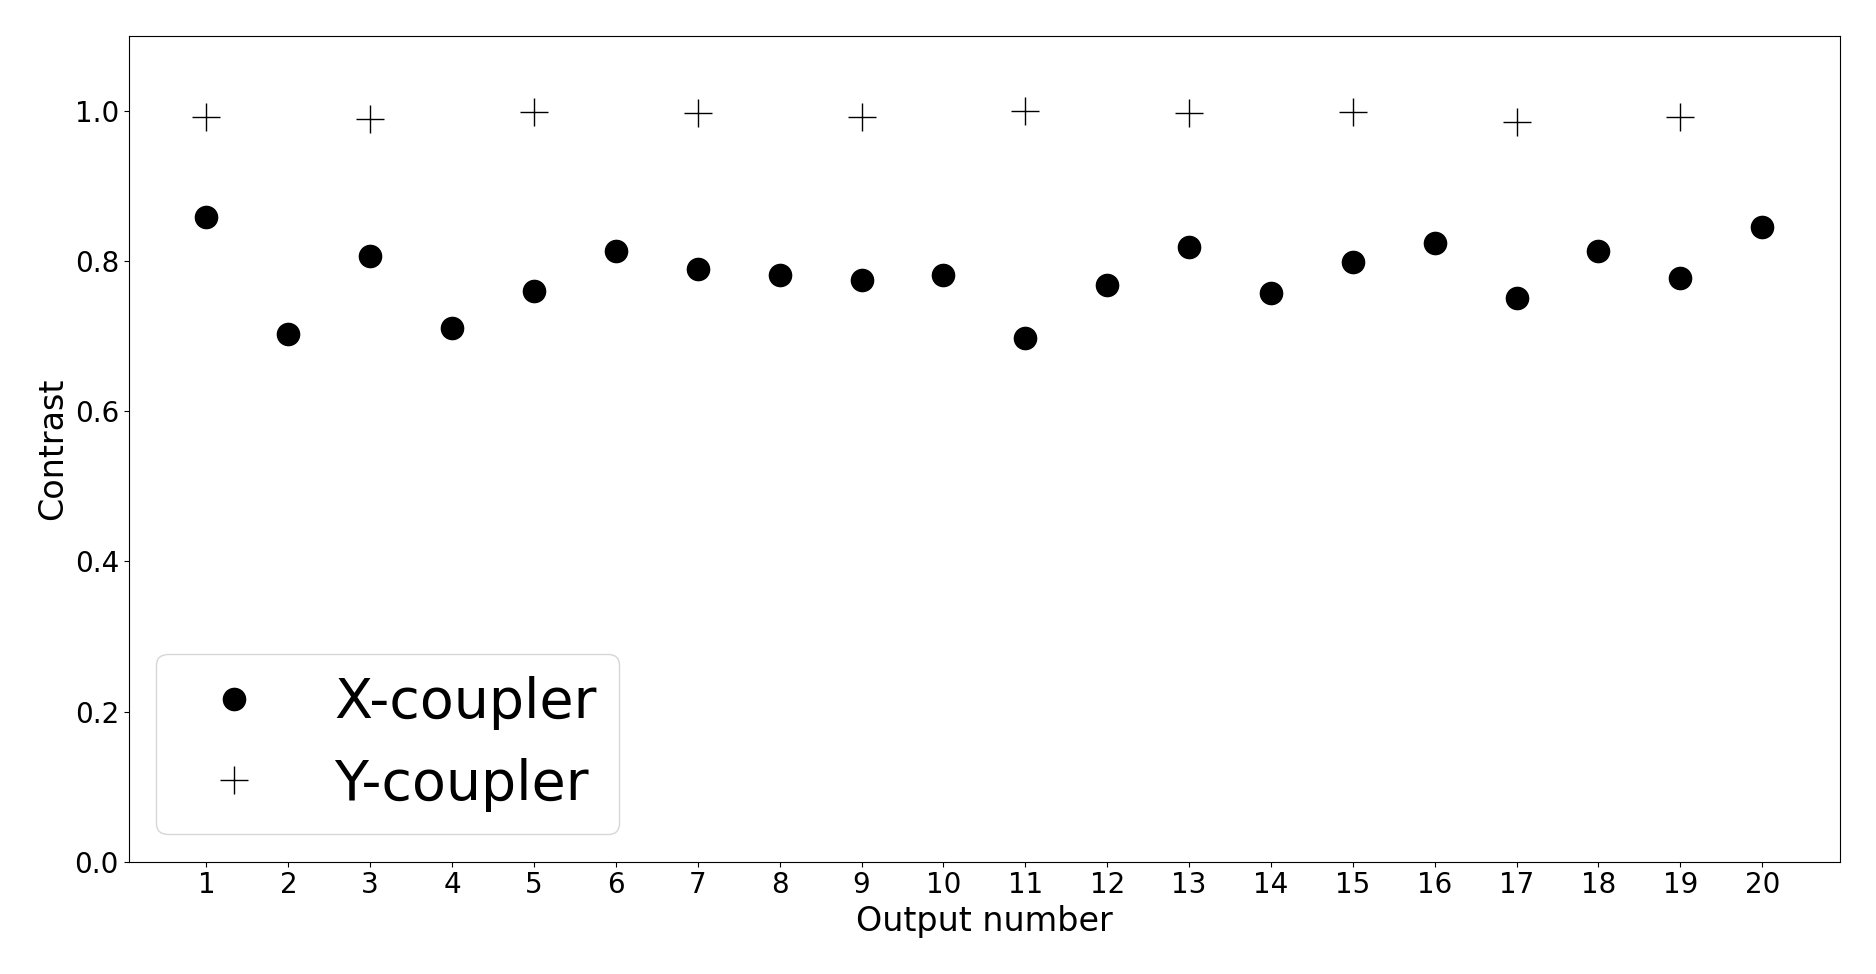
\includegraphics[width=\figwidth]{Figure_Chap2/ContrastComparison_20201124_20201119_LaTex.png}
    \caption[Contraste interférométrique estimé pour toutes les bases avec les puces $X$ et $Y$.]{Contraste interférométrique estimé pour toutes les bases avec les puces $X$ (représenté par les points) et $Y$ (représenté par les croix).}
    \label{fig:ChipContrast}
\end{figure}


% Conclusion
\threesubsection{Conclusion sur la caractérisation}

En résumé, j'ai mesuré un niveau de \textit{cross-talk} équivalent pour les deux puces, mais un contraste interférométrique dégradé de $\sim 20\%$ sur les mesures de la puce $X$. De plus, les transmissions des puces $X$ et $Y$ sont estimées à $30\%$ et $13\%$, respectivement. Le facteur $2$ observé entre les transmissions des deux puces est attendu du fait des natures transmissives différentes des coupleurs directionnel et des jonctions $Y$. La puce $X$ offre ainsi le double avantage, premièrement, d'être plus transmissive et, deuxièmement, de disposer de deux points de mesures des franges déphasés de $\pi \,$rad sur chaque image acquise, permettant de diviser par 2 la quantité de données nécessaire (plus de détails dans la section~\ref{sec:Modulation}).

On peut alors conclure qu'il sera préférable d'utiliser la puce $X$ lors de futurs prises de données, mais comme nous le verrons dans la section~\ref{sec:BinaryCharac}, je ne suis pas parvenu à estimer les observables interférométriques avec cette puce et la puce $Y$ produit de bien meilleurs résultats.

Ainsi, les valeurs de transmission mesurées sont suffisantes pour permettre leur intégration et de les tester sur le banc \ac{SCExAO} en conditions d'observations du ciel, ce que j'ai pu faire durant ma thèse et que j'exposerai dans la section~\ref{sec:FIRSTv2Subaru}. En revanche, elles ne sont pas suffisantes pour une exploitation de l'instrument \ac{FIRSTv2} ouverte à la communauté scientifique. Guillermo Martin et Manon Lallement travaillent à Grenoble sur le développement de nouvelles puces avec de meilleures performances. Par exemple, des puces fabriquées avec un dopage aux ions Ag+, augmentant le contraste d'indice des guides ce qui permet des rayons de courbure plus petits. Le but est de faire les croisements avec des angles plus grands afin de diminuer le \textit{cross-talk}. Mais aussi, des puces 3D \citep{martin2022a} dont les guides d'onde ont été gravés par laser non pas dans un même plan mais dans le volume de la puce, permettent d'éviter les croisements qui engendrent le \textit{cross-talk} et les pertes en transmission. De même, des puces avec une modulation électro-optique fabriquées par \textit{FEMTO-ST}\footnote{\url{https://www.femto-st.fr/en}} dans un matériau différent (Niobate de Lithium LiNi) avec une meilleure transmission ont été caractérisées sur le banc de test \ac{FIRSTv2} durant ma thèse \citep{martin2022b}. Enfin, des puces utilisant différents types de coupleurs (ABCD, directionnel asymétrique) dont les paramètres physiques sont explorés ont été fabriquées et caractérisées dans \cite{lallement2022}.


%%%%%%%%
\subsubsection{La polarisation}

Les deux polarisations ne sont pas transmises de la même façon à travers les composants d'optique intégrée. En effet, en plaçant un prisme de Wollaston en sortie de la puce (juste après le réseau holographique) pour imager les deux polarisations et un polariseur en entrée de la puce (juste avant la matrice de micro-lentilles) que l'on place successivement sur les deux polarisations, on peut estimer la façon dont les deux polarisations se propagent dans la puce. On note que le prisme de Wollaston ne peut pas être réglé en rotation autour de son axe $Z$, contrairement au polariseur en entrée. La figure~\ref{fig:PolaComparison} présente le flux des $20$ sorties de la puce $Y$ ($10$ pour chaque polarisation) lorsque le polariseur sélectionne la polarisation verticale (V) (dénommée ici \og Pola X \fg) sur l'image de gauche, lorsque le polariseur est enlevé du chemin optique sur l'image du milieu et lorsque le polariseur sélectionne la polarisation horizontale (H) (dénommée ici \og Pola Y \fg) sur l'image de droite. Les flèches bleues et rouges identifient les polarisation V et H séparées par le prisme de Wollaston, respectivement. La source utilisée ici est la source SLED 650 fabriquée par \textit{Exalos Inc.}\footnote{\url{https://www.exalos.com/}} de largeur spectrale mesurée de $\sim 10 \,$nm. Ce qu'on peut déduire de ces mesures c'est que premièrement, lorsque le polariseur sélectionne l'une ou l'autre des polarisations à l'injection de la puce, on mesure une intensité lumineuse sur les sorties dans les deux polarisations discriminées par le prisme de Wollaston (et aucune position du polariseur ne permet d'annuler totalement le flux d'une des deux moitiés des sorties sur la caméra). Il semblerait qu'une partie de la polarisation sélectionnée est projetée dans l'autre polarisation au cours de la transmission dans la puce. Deuxièmement, on remarque qu'il y a moins de flux converti dans l'autre polarisation lorsque c'est la polarisation V qui est sélectionnée par le polariseur en entrée de la puce.

\begin{figure}[ht!]
    \centering
    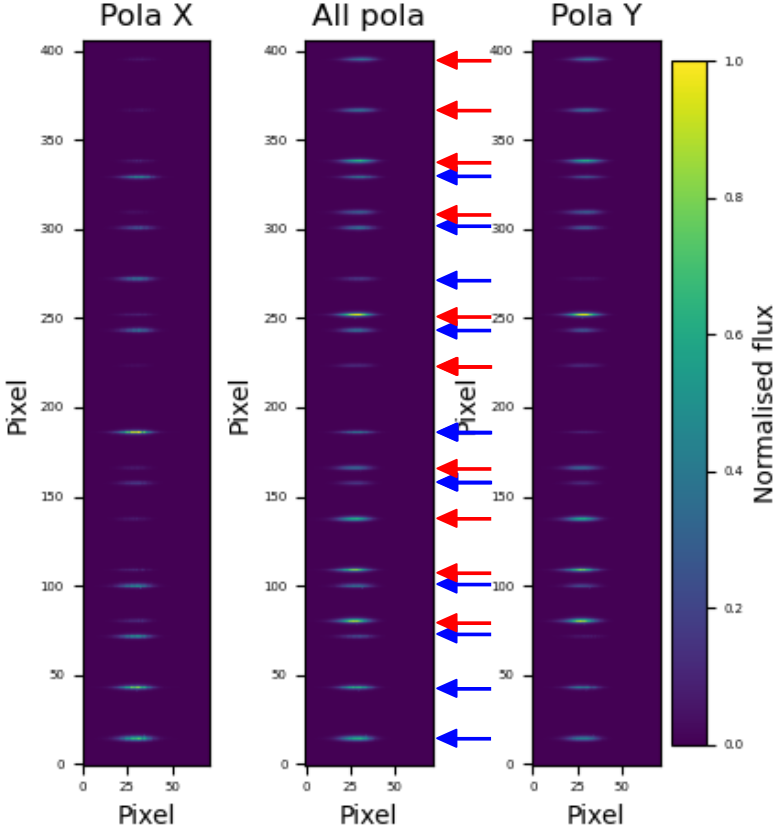
\includegraphics[width=0.7\textwidth]{Figure_Chap2/20210707_PolaComparison_PolId.png}
    \caption[Images de la caméra montrant le flux sur les dix sorties de la puce $Y$ dans les deux polarisations.]{Images de la caméra montrant le flux normalisé par le maximum de l'image sur les dix sorties de la puce $Y$ (multiplié par deux par le prisme de Wollaston), lorsque le polariseur en amont de la puce sélectionne la polarisation V (à gauche), est retiré (au milieu) et sélectionne la polarisation H (à droite). Dans les titres, les polarisations V et H sont nommées X et Y, respectivement et l'axe horizontal est l'axe de dispersion. Les flèches bleues et rouges identifient la polarisation V et H, respectivement.}
    \label{fig:PolaComparison}
\end{figure}

Ainsi, lors de l'intégration du polariseur sur le banc de test, l'angle de celui-ci est réglé sur la polarisation V et affiné de façon à minimiser le flux observé sur les sorties dans la polarisation H sur l'image de la caméra. La figure~\ref{fig:PolaRotation} montre l'intensité lumineuse moyenne de toutes les sorties de la puce $X$, en polarisation V en trait continu et en polarisation H en trait-point, en fonction de l'angle du polariseur. La polarisation V est sélectionnée lorsque l'angle du polariseur est égal à $\sim -15\degree$. Ce graphique permet de quantifier l'échange de polarisation dans la puce photonique et on voit que la polarisation H (angle du polariseur égal à $\sim 75\degree$) est celle dont le flux est le plus converti dans la polarisation opposée (V). On souhaite donc placer le polariseur à l'angle égal à $\sim 0\degree$ qui sélectionne la polarisation V. Autrement dit, on souhaite régler l'angle du polariseur qui minimise le flux dans la polarisation opposée à celle qu'il sélectionne.

\begin{figure}[ht!]
    \centering
    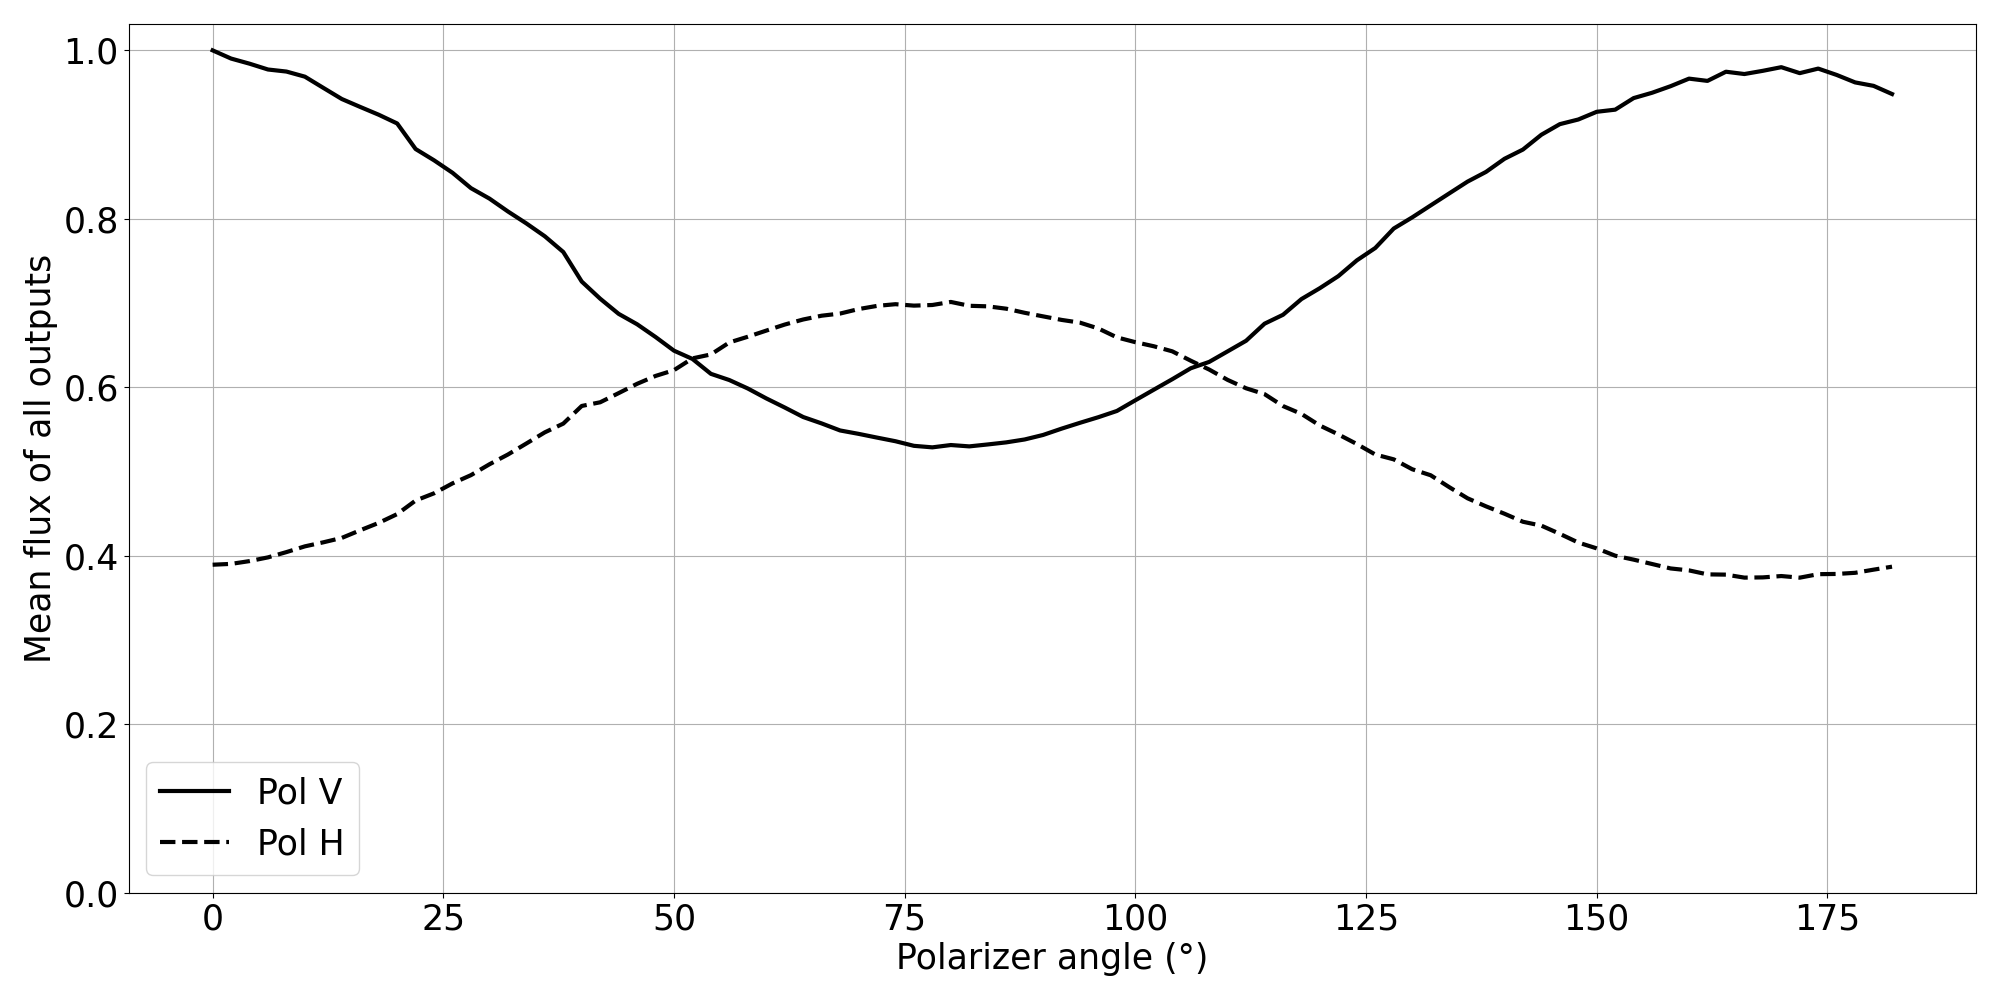
\includegraphics[width=\figwidth]{Figure_Chap2/20221019_5TC_PX_OutputFlux_Mean_VS_Angle.png}
    \caption[Flux intégré moyenné sur toutes les sorties de la puce $X$ en fonction de l'angle du polariseur, dans les deux polarisations.]{Flux intégré moyenné sur toutes les sorties de la puce $X$, sur toute la gamme spectrale transmise, en polarisation V (en trait continu) et en polarisation H (en trait discontinu) sélectionnées par le prisme de Wollaston, en fonction de l'angle du polariseur en amont de la puce. Les courbes sont normalisées par le maximum des deux (le premier point de la courbe en polarisation V).}
    \label{fig:PolaRotation}
\end{figure}

Des travaux sont actuellement en cours par Harry-Dean Kenchington Goldsmith et Manon Lallement, afin d'améliorer notre compréhension du comportement de la polarisation dans les puces photoniques. À ce jour nous pensons que les axes principaux des guides de la puce ne sont pas alignés avec les axes de toutes les fibres optiques ainsi que du polariseur en entrée et du prisme de Wollaston. Cela a pour conséquence de rendre la polarisation elliptique et expliquerait les mesures montrées sur le graphique de la figure~\ref{fig:PolaRotation}. Ce sujet est lié aux problèmes de \wiggles~que nous discuterons par la suite dans la section~\ref{sec:wiggles}. De plus, de récentes analyses montreraient que la biréfringence des fibres optiques ai un effet sur la polarisation des faisceaux injectés. Cela constitue une source de perturbations à prendre en compte dans l'analyse présentée ici.


%%%%%%%%%%%%%%%%
\subsection{Le spectro-imageur}
\label{sec:InstruSpectro}

Le principe optique du spectro-imageur du banc de test a été changé au cours de ma thèse dans le but d'augmenter sa résolution spectrale. À l'origine, il était composé d'un objectif de microscope, d'un prisme de Wollaston, d'un prisme équilatéral en SF2 et d'une lentille d'imagerie et fournissait une résolution spectrale égale à $\sim 600$. Durant son stage en 2021, Manon Lallement a spécifié, optimisé et intégré au banc le nouveau concept de spectro-imageur. Les caractéristiques requises (récapitulées dans la deuxième colonne du tableau~\ref{tab:SpectroSpec}) étaient (CR1) d'imager une bande spectrale égale à $\Delta \lambda = 140 \,$nm (entre $633 \,$nm et $773 \,$nm) sur moins que la largeur de la caméra; (CR2) que la résolution spectrale $\lambda / \delta \lambda$ soit égale à $2\,200$ pour $\lambda = 656,3 \,$nm; (CR3) que les sorties dans les deux polarisations ne se superposent pas lorsqu'elles sont imagées sur la caméra.

\begin{table}[ht!]
    \centering
    \renewcommand*{\arraystretch}{1}
    \begin{tabular}{|c|c|c|}
        \hline
        Composant & Spécification & Solution \\
        \hline
        Source & N/A & V-Groove de séparation de $127 \,$\um\\
        \hline
        \multirow{5}{*}{Collimateur} & \multirow{5}{*}{N/A} & objectif de microscope Thorlabs TL2X SAP \\
         & & NA $= 0,1$ \\
         & & distance de travail d$= 56,3 \,$mm \\
         & & focale $\text{f'} = 100\,$mm \\
         & & grossissement $\times 2$ \\
        \hline
        \multirow{2}{*}{Wollaston} & \multirow{2}{*}{N/A} & dimensions $50 \times 50 \times 11,4\,$mm \\
         & & séparation $10,8' = 0,18\degree$ \\
        \hline
        \multirow{2}{*}{Réseau} & \multirow{2}{*}{(CR1), (CR2)} & holographique en transmission \\
         & & fréquence spatiale $600 \,\text{l}.\text{mm}^{-1}$\\
        \hline
        \multirow{3}{*}{Imageur} & \multirow{3}{*}{(CR1), (CR2), (CR3)} & objectif de Lister de focale $83 \,$mm (deux lentilles) \\
         & & $\text{f'}_1 = 150 \,$mm \\
         & & $\text{f'}_2 = 80 \,$mm \\
        \hline
        \multirow{3}{*}{Caméra} & \multirow{3}{*}{N/A} & Andor Zyla 5.5 USB 3.0 \\
         & & taille des pixels $6,5 \,$\um \\
         & & $2\,560 \,$px en largeur \\
        \hline
    \end{tabular}
    \caption[Spécifications de conception et caractéristiques des composants du nouveau spectro-imageur.]{Spécifications de conception et caractéristiques des composants du nouveau spectro-imageur. Le type de composant est indiqué dans la colonne de gauche, la caractéristique requise est rappelée dans la colonne du milieu (N/A est indiqué lorsque le composant existait déjà au laboratoire) et les caractéristiques finales du composant sont présentées dans la colonne de droite. CR1 : imager une bande spectrale égale à $\Delta \lambda = 160 \,$nm (entre $623 \,$nm et $781 \,$nm) sur moins que la largeur de la caméra ($1430 \,$px). CR2 : la résolution spectrale $\lambda / \Delta \lambda$ doit être égale à $2\,200$ pour $\lambda = 656,3 \,$nm. CR3 : les sorties dans les deux polarisations ne doivent pas se superposer lorsqu'elles sont imagées sur la caméra.}
    \label{tab:SpectroSpec}
\end{table}

Les caractéristiques des composants choisis pour la solution du nouveau spectro-imageur sont récapitulées dans la colonne de droite du tableau~\ref{tab:SpectroSpec}. Les composants dont la spécification n'est pas renseignée sont ceux qui étaient déjà disponibles au laboratoire, constituant les paramètres fixés de l'optimisation de la conception du spectro-imageur.

La figure~\ref{fig:SpectroPhoto} montre une photographie du nouveau spectro-imageur après intégration sur le banc de test. La source est le V-Groove (1) sur lequel sont branchées les fibres optiques de sortie de la puce photonique. Les faisceaux des fibres sont ensuite collimatés par un objectif de microscope (2) fabriqué par \textit{Thorlabs}\footnote{\url{https://www.thorlabs.com/}} qui a un grossissement $\times 2$. L'élément de dispersion (3) choisi est un réseau \ac{VPH} fabriqué par \textit{Wasatch Photonics}\footnote{\url{https://wasatchphotonics.com/}}, que j'appelle réseau holographique dans tout le manuscrit, de fréquence spatiale égale à $600 \,\text{l}.\text{mm}^{-1}$. Celui-ci travaille en transmission et est constitué d'une couche de gélatine photosensible dans laquelle le réseau de diffraction a été gravé au laser. Cette couche est confinée entre deux parois de verre en BK7 traitées en surface avec un revêtement anti-réflection pour les longueurs d'onde du visible. Le prisme de Wollaston (4) est fabriqué par \textit{Optique Fichou}\footnote{\url{https://optique-fichou.com/}} et les nouvelles optiques ont été dimensionnées en s'assurant que les sorties de la puce photonique imagées sur la caméra, après la séparation des polarisations par le prisme, soient séparées d'environ $5 - 8 \,$px sur l'axe vertical pour éviter une superposition du flux de deux sorties adjacentes. Le système imageur juste avant la caméra doit avoir une focale de $83 \,$mm pour répondre aux performances attendues et il a été choisi d'installer un objectif de Lister\footnote{\url{https://www.degruyter.com/document/doi/10.1515/aot-2019-0002/html}} afin de limiter les aberrations optiques, composé de deux lentilles (5) et (6) de focales égales à $150 \,$mm et $80 \,$mm, respectivement, disposées à $80 \,$mm l'une de l'autre. Enfin, la caméra (7) est de la gamme Andor Zyla $5.5$ disposant de $2\,560 \,$px de taille égale à $6,5 \,$\um. Le nombre de pixels choisis sur lesquels la bande spectrale est imagée est de $1\,430 \,$px ce qui permet d'intégrer le spectro-imageur sur le banc \ac{SCExAO} avec des caméras de tailles différentes, sans changer son concept et la largeur de la bande spectrale imagée.

\begin{figure}[ht!]
    \centering
    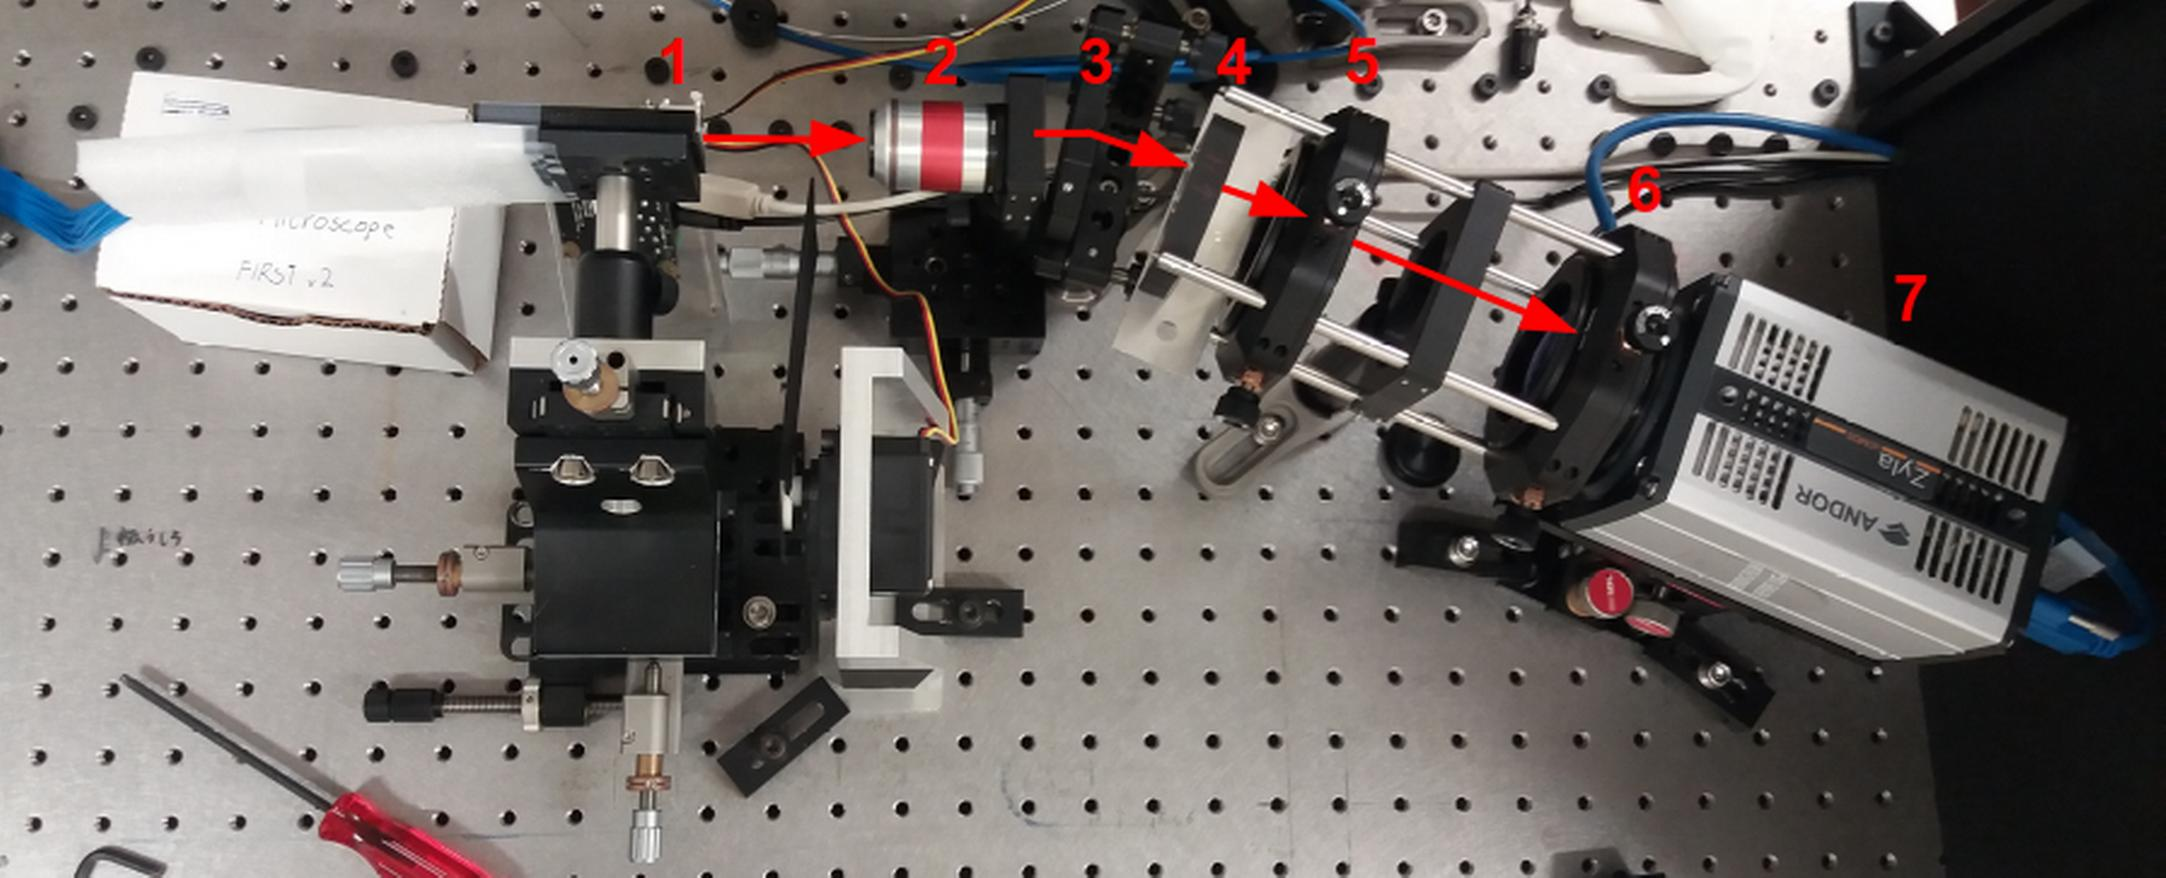
\includegraphics[width=\figwidth]{Figure_Chap2/20210817_Spectro04.jpg}
    \caption[Photographie du spectro-imageur du banc de test de FIRSTv2.]{Photographie du spectro-imageur du banc de test de FIRSTv2. Les composants sont numérotés comme suit : (1) le V-Groove branché aux fibres de sorties de la puce photonique; (2) l'objectif de microscope de collimation (grossissement $\times 2$); (3) le réseau holographique; (4) le prisme de Wollaston; (5) la première lentille d'imagerie de focale égale $150 \,$mm; (6) la deuxième lentille d'imagerie de focale égale à $80 \,$mm; (7) la caméra.}
    \label{fig:SpectroPhoto}
\end{figure}

La caméra de la gamme ORCA-Quest qCMOS fabriquée par \textit{Hamamatsu}\footnote{\url{https://www.hamamatsu.com/}} a récemment été acquise et est intégrée dans \ac{FIRSTv1} au télescope Subaru. Elle dispose de meilleurs performances que la caméra utilisant la technologie \ac{EMCCD} jusqu'ici utilisée : entre autre, l'écart-type sur le bruit de courant d'obscurité est égal à $0,006 \,\text{e}^-.px^{-1}.s^{-1}$ et l'efficacité quantique est de $65 - 80\%$ dans la gamme $600 - 700\,$nm. Le capteur est composé de $4\,000 \times 2\,300 \,$px et les pixels ont une taille égale à $4,6 \,$\um. Cela nous permettrait d'augmenter, à terme, la résolution spectrale, lorsque la transmission de l'instrument sera plus élevée, ce qui est un atout non négligeable pour l'étude de protoplanètes, comme nous l'avons vu dans la section~\ref{sec:Protoplanetes}.

L'analyse des mesures effectuées pour l'étalonnage spectral de l'instrument, présentés dans la section~\ref{sec:EtalonnageSpectral}, permet d'estimer la résolution spectrale du nouveau spectro-imageur à $\sim 3\,400$. Celle-ci est plus élevée que prévu car les composants ont été alignés à l'aide du visionnage de l'image de la caméra ce qui ne permet pas de s'assurer que les spots lumineux aient une taille de $2 \,$px a minima (pour respecter le critère de Shanon). Comme nous le verrons par la suite, cela n'empêche pas de caractériser la source protoplanétaire simulée présentée plus loins dans la section~\ref{sec:SystBinaire} car la source utilisée pour le compagnon a une largeur spectrale s'étendant sur plus de quatre pixels.


%%%%%%%%%%%%%%%%
\subsection{La caméra}
\label{sec:InstruCamera}

% Brève description
La caméra utilisée sur le banc \ac{FIRSTv2} est de la gamme Andor Zyla $5.5$ fabriquée par \textit{Oxford Instruments}\footnote{\url{https://www.oxinst.com/}}. Elle utilise la technologie de capteur \ac{CMOS}, d'une taille de $2\,160 \,\text{px} \times 2\,560 \,\text{px}$ de taille de pixel égale à $6,5 \,$\um. Ses caractéristiques sont résumées dans le tableau~\ref{tab:CameraSpec}. Elle est refroidie par air à l'aide d'un ventilateur. Le spectro-imageur et la caméra sont isolés des lumières parasites de la pièce grâce à un coffrage en carton amovible (l'ordinateur de contrôle étant dans la même pièce). La caméra est opérée avec le mode obturateur déroulant (\textit{rolling shutter}) de lecture des pixels à une fréquence de $280 \,$MHz. Les charges des pixels de chaque image sont donc lues en $3,6 \,$ns, garantissant que les franges ne sont pas brouillées pendant l'acquisition d'une image.

\begin{table}[ht!]
    \centering
    \renewcommand*{\arraystretch}{1}
    \begin{tabular}{cc}
        \hline
        \hline
        \multicolumn{2}{c}{Caractéristiques du détecteur} \\
        \hline
        \hline
        Technologie & CMOS \\
        Connexion & USB $3.0$ \\
        Nombre de pixels & $2\,160 \times 2\,560$ \\
        Taille des pixels & $6,5 \,$\um \\
        Efficacité quantique max & $60$\% \\
        Efficacité quantique $> 30 \%$ & $400 - 800 \,$nm \\
        Mode de lecture & \textit{Rolling shutter} \\
        Fréquence de lecture & $280 \,$MHz \\
        Sensibilité & $0,49 \, \text{e}^- \,$/ADU \\
        Bruit de lecture & $1,11 \, \text{e}^- \,$RMS \\
        Courant d'obscurité & $0,1453 \, \text{e}^{-}.\text{px}^{-1}.\text{s}^{-1}$ \\
        Dynamique & $65\,536:1$\\
        \hline
    \end{tabular}
    \caption[Caractéristiques de la caméra Andor Zyla 5.5 USB 3.0 du banc de test de FIRSTv2.]{Caractéristiques de la caméra Andor Zyla 5.5 USB 3.0 du banc de test de FIRSTv2.}
    \label{tab:CameraSpec}
\end{table}

% Image de Dark
La figure~\ref{fig:CameraDark} présente la médiane de cent images de la caméra sans flux, à un temps d'exposition de $100 \,$ms. Cette image permet d'étalonner le bruit sur le courant d'obscurité et le bruit de lecture de la caméra sur toutes les données acquises (pour plus de détails voir la section~\ref{sec:CameraDark}). On remarque des motifs par colonne visibles aussi sur la visualisation en temps réel du capteur de la caméra. Ce sont des motifs fixes qui résultent de la structure de l'électronique d'amplification des pixels inhérente aux capteurs \ac{CMOS}\footnote{\url{https://www.mdpi.com/2076-3417/10/11/3694/htm}}. Ces structures étant constantes en fonction du temps, elles se corrigent très bien lors du traitement de données.

\begin{figure}[ht!]
    \centering
    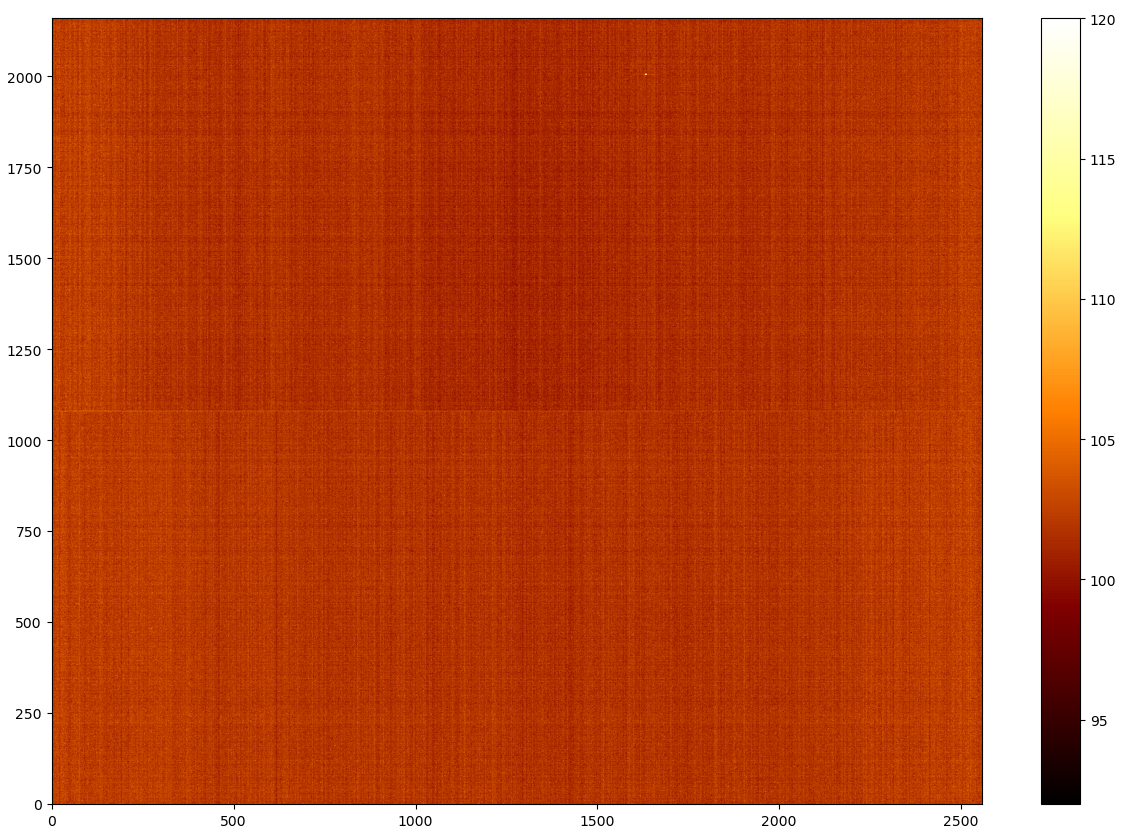
\includegraphics[width=\figwidth]{Figure_Chap3/20220705_DarkFullImage_100ms_24C_median.png}
    \caption[Image sans flux de la caméra Andor Zyla de FIRSTv2.]{Médiane de cent images de temps d'exposition égal à $100 \,$ms de la caméra Andor Zyla, sans flux. Les valeurs des pixels données sur les échelles sont en \ac{ADU}.}
    \label{fig:CameraDark}
\end{figure}

% Calcul du SNR
Le rapport signal sur bruit obtenu ou \ac{SNR} sur les images de la caméra avec un temps d'exposition t et pour un flux de photons P, s'écrit :

\begin{equation}
    \text{SNR} = \frac{\eta \times \text{P} \times \text{t}}{\sqrt{\sigma_{lec}^{2} + \sigma_{obsc}^{2} + \sigma_{p}^{2}}}
\end{equation}

\noindent avec $\eta$ l'efficacité quantique, $\sigma_{lec} = 1,11 \,\text{e}^-$ l'écart-type du bruit de lecture, $\sigma_{obsc} = \sqrt{\text{t} \times 0,1453 \,\text{e}^-.px^{-1}.s^{-1}}$ l'écart-type du bruit sur le courant d'obscurité et $\sigma_{p} = \sqrt{\eta \times P \times t}$ l'écart-type du bruit de photons. Les capteurs de type \ac{CMOS} actuellement fabriqués remplacent petit à petit les capteurs \ac{CCD} qui étaient incontournables ces dernières décennies. En effet, les capteurs \ac{CMOS} consomment moins d'énergie, sont plus rapides lors de la lecture des charges des pixels du capteur et présentent un bruit de courant d'obscurité et de lecture bien plus faibles. La caméra de \ac{FIRSTv1} utilise la technologie \ac{EMCCD} qui dispose d'un gain d'amplification du signal mais, comparée à la technologie \ac{CMOS}, cela nécessite un fort gain induisant une faible dynamique et un bruit d'amplification est ajouté (voir plus de détails dans la section 2.1.1.3 de la thèse d'Elsa Huby \cite{huby2013these}).

% Par exemple, l'équipe travaillant sur \ac{SCExAO} a pu montré que leur caméra fabriquée par \textit{Hamamatsu}\footnote{\url{https://www.hamamatsu.com/eu/en.html}} comptait les photons incident au capteur (de type \ac{CMOS}). Comme le montre le graphique de la figure~\ref{fig:HamamatsuSCExAO}, qui est le nombre d'occurrence (axe des ordonnées) des valeurs d'\ac{ADU} (axe des abscisses) mesurées à faible intensité lumineuse, le bas bruit permet d'atteindre une résolution sur la mesure de l'intensité lumineuse pour mesurer.
% First, we've tried photon counting in the lab in Hilo with one of the Hamamatsu cameras. Attached is a histogram of pixel counts in the near-dark and another in the slightly less dark. #of occurence (y-axis) vs. px value in ADU (x-axis). Blue is the standard readout mode (fast) and orange is the "ultraquiet readout". As you can see, we're counting photons with probably just a few percent of errors due to the feet of each lobe.
% \begin{figure}[ht!]
%     \centering
%     \includegraphics[width=\figwidth]{Figure_Chap3/}
%     \caption[]{}
%     \label{fig:HamamatsuSCExAO}
% \end{figure}

Ainsi, les bruits de lecture et sur le courant d'obscurité sont négligeables par rapport au bruit de photons (dans le régime de flux élevé), le \ac{SNR} peut se ré-écrire comme suit :

\begin{equation}
    \text{SNR} = \sqrt{\eta \times \text{P} \times \text{t}}
\end{equation}

Les détecteurs permettent aujourd'hui l'acquisition de données très peu affectées par le bruit instrumental et le \ac{SNR} est donc uniquement limité par le bruit de photons. La technique d'interférométrie \textit{nulling} qui permet de s'affranchir du bruit de photon de l'étoile, se révèle alors très pertinente et constitue l'avenir du projet \ac{FIRST}.


%%%%%%%%%%%%%%%%%%%%%%%%%%%%%%%%
\section{Le logiciel de contrôle}
\label{sec:ControlSoftware}

%%%%%%%%%%%%%%%%
\subsection{L'architecture}

Une partie du travail de ma thèse a consisté en l'amélioration du logiciel de contrôle du banc de test \ac{FIRSTv2}, écrit en Python\footnote{\url{https://www.python.org/}}. Il s'agissait d'une part de faire la mise à jour des programmes depuis la version $2.7$ vers la version $3.9$ de Python (avec l'aide précieuse de Pierre Fedou, Franck Marchis et Clément Chalumeau), ce qui n'est pas évident surtout vis-à-vis des \ac{SDK} associées aux composants, fournis par les constructeurs. Le \ac{SDK} du miroir déformable \textit{Iris AO} que nous avons adapté à la version $3+$ de Python est disponible sur GitHub\footnote{\url{https://github.com/scexao-org/Iris-AO_MEMS_Software-control.git}} et celui de la caméra est fourni directement par \textit{Andor}. D'autre part, il s'agissait de changer toute l'architecture du logiciel car un unique script (dont un schéma est présenté sur la figure~\ref{fig:SoftwareArchitecture} du haut) était exécuté pour établir la connexion et contrôler tous les composants (\ac{MEMS}, \ac{ODL} et caméra), ce qui induisait une lenteur dans l'utilisation du terminal de commande par l'opérateur. Sur le schéma, chaque rectangle jaune correspond à un script et décrit son contenu. Certaines parties du logiciel étaient écrites dans d'autres scripts comme \texttt{memsCtrl.py} et \texttt{odlCtrl.py} mais étaient exécutés dans le script principal. Les rectangles bleus clairs représentent des connexions entre processus/processus ou processus/composants et les rectangles bleus foncés représentent les composants.

\begin{figure}[ht!]
    \centering
    \begin{subfigure}{1\textwidth}
        \centering
        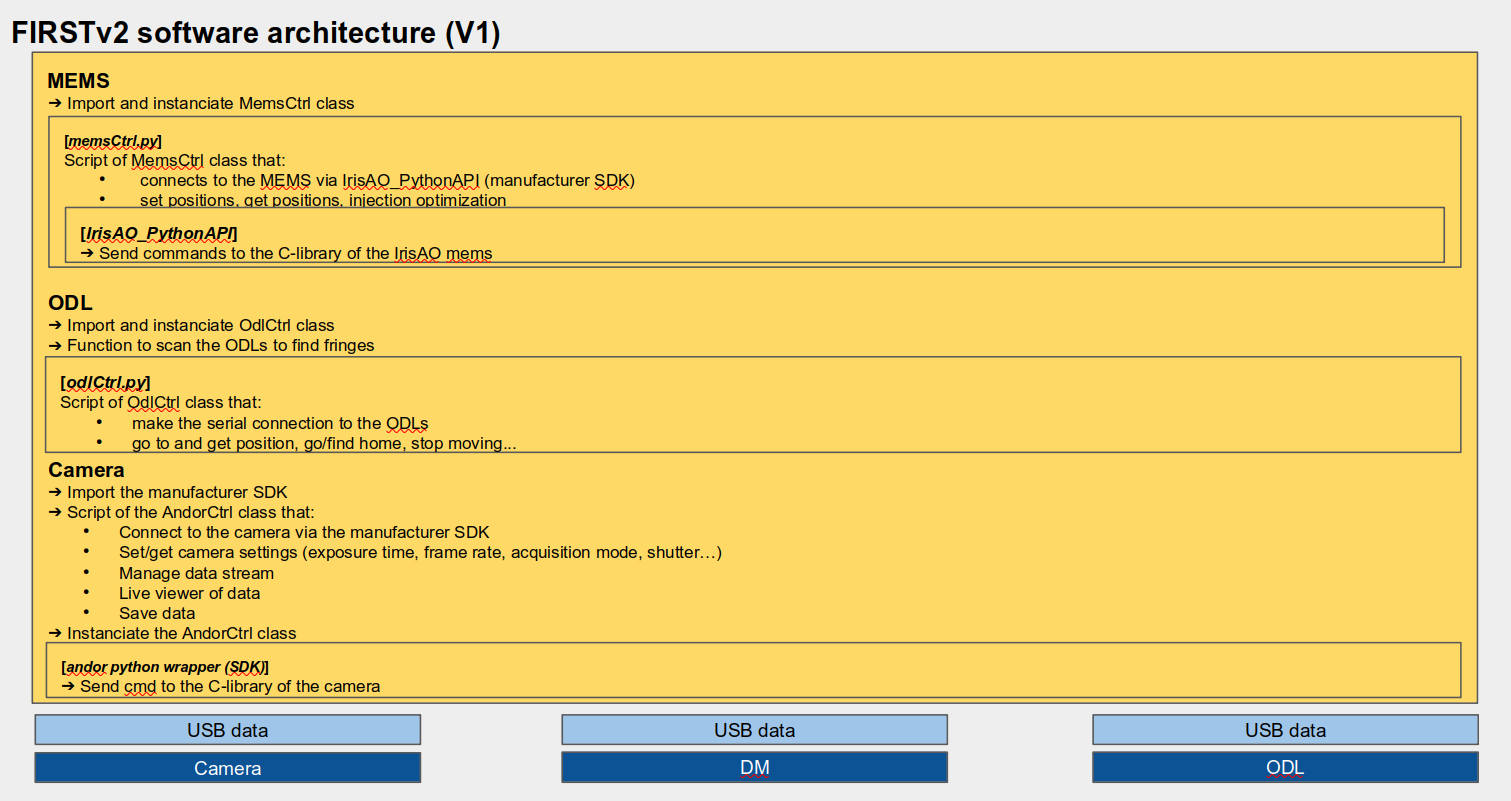
\includegraphics[width=\textwidth]{Figure_Chap2/SoftwareArchitecture_FIRSTv2_v1.png}
    \end{subfigure}
    \line(1,0){430}\\
    \begin{subfigure}{1\textwidth}
        \centering
        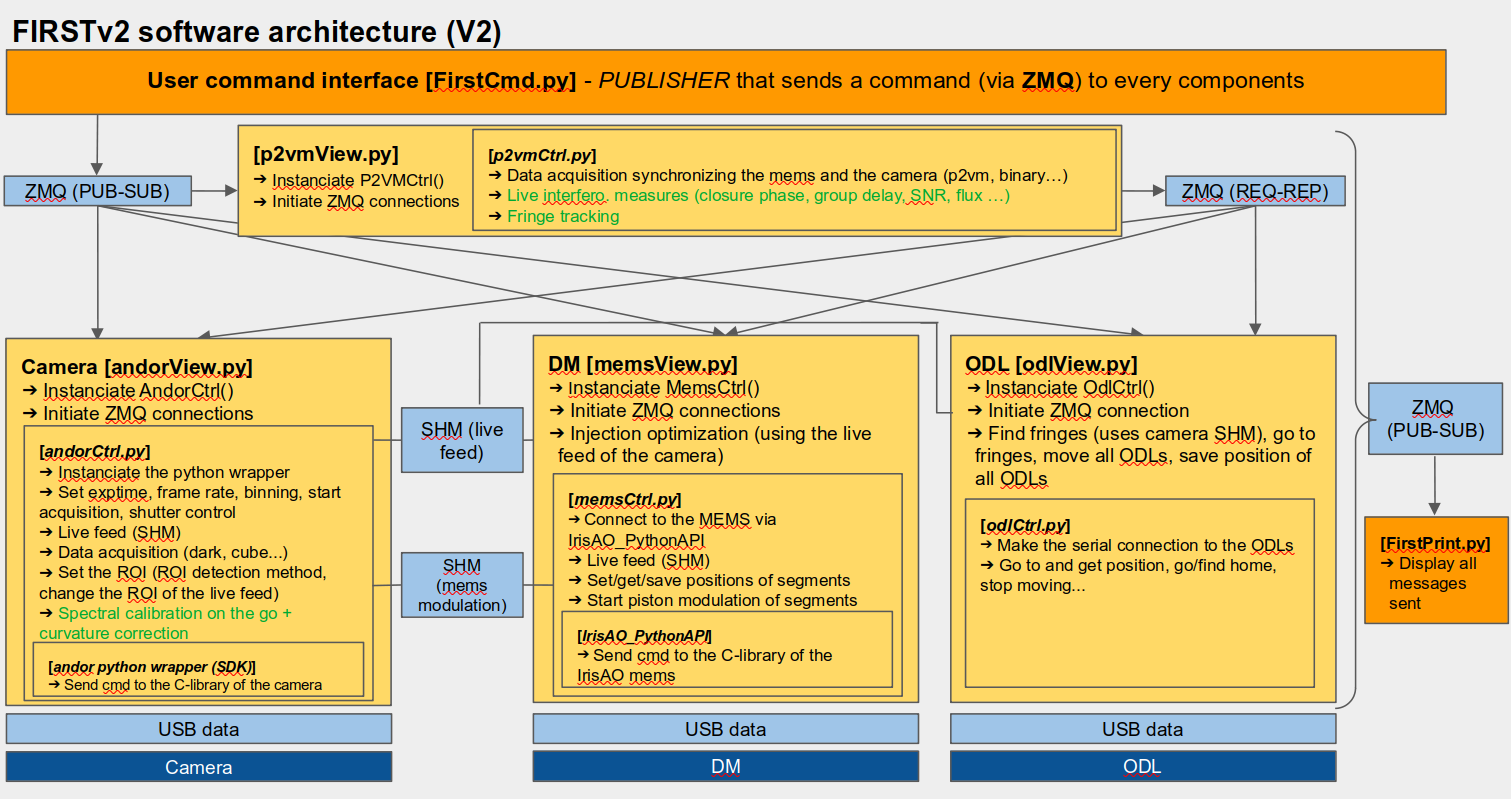
\includegraphics[width=\textwidth]{Figure_Chap2/SoftwareArchitecture_FIRSTv2_v2.png}
    \end{subfigure}
    \caption[Schémas de l'architecture du logiciel de contrôle de FIRSTv2 avant et après ma thèse.]{Schémas de l'architecture du logiciel de contrôle de FIRSTv2 avant (en haut) et après (en bas) ma thèse. Les rectangles jaunes sont des scripts, les rectangles oranges sont les scripts qui implémentent une interface utilisateur, les rectangles bleus clairs sont des interfaces et les rectangles bleus foncés sont les composants. Les flèches montrent les liens établis entre les différents processus et ce qui est écrit en vert est ce qui n'est pas encore implémenté.}
    \label{fig:SoftwareArchitecture}
\end{figure}

La figure~\ref{fig:SoftwareArchitecture} du bas présente le schéma de cette nouvelle architecture, avec les mêmes codes couleurs que celui du haut, précédemment décrit et où les flèches indiquent une interaction entre processus. J'ai ainsi amélioré l'architecture du logiciel en créant un script pour chaque composant afin de les exécuter en parallèle. Les rectangles oranges sont des terminaux d'interface logiciel/utilisateur. Le terminal nommé \textit{User command interface} permet de centraliser l'envoi de toutes les commandes vers les différents processus par l'opérateur, via des protocoles de communication serveur/client (voir plus de détails dans la section~\ref{sec:ZMQ}) et le terminal nommé \texttt{FirstPrint.py} centralise l'affichage de tous les messages de tous les processus. Toutes les fonctions de bas niveau permettant d'établir la connexion et de contrôler les composants sont dans un script nommé \texttt{XCtrl.py} et sont importés dans un script nommé \texttt{XView.py} (\texttt{X} étant le nom du composant) qui les exécute et implémente des fonctions de plus haut niveau, comme l'optimisation de l'injection par le \ac{MEMS}. Ce sont ces derniers scripts qui sont exécutés lors du démarrage du logiciel de contrôle.

De plus, par rapport à l'ancienne version du logiciel, un processus nommé \texttt{p2vmView.py} qui n'est pas directement lié à un composant a été ajouté. Il fonctionne avec la même architecture que les autres programmes liés aux composants et permet l'envoi successif de commandes à la caméra, au \ac{MEMS} et aux \ac{ODL}s, via également des protocoles de communication serveur/client (démarrer une acquisition d'images, changer les positions des segments du \ac{MEMS}, envoyer les \ac{ODL}s en position de zéro \ac{OPD}, etc...). C'est ce processus qui fait l'acquisition automatique des données (une soixantaine de fichiers d'images) permettant de calculer les \ac{V2PM} et \ac{P2VM} ainsi que les données interférométriques (moins d'une dizaine de fichiers d'images) sur la source protoplanétaire simulée (voir plus de détails dans la section~\ref{sec:SystBinaire}). Les fonctionnalités écrites en vert sont celles qui ne sont pas encore implémentées.

Enfin, pour la visualisation en temps réel des données (les images de la caméra et la carte de phase de la surface du miroir segmenté) j'utilise un système de mémoire partagée sur l'ordinateur, nommé \ac{SHM} sur le schéma (voir plus de détails dans la section~\ref{sec:SHM}). Par exemple, le processus associé à la caméra envoie les images dans une mémoire partagée allouée et un autre processus récupère les images de cet espace mémoire en la lisant et les affiche. Cela permet aussi de transmettre des données entre les différents programmes en cours d'exécution.

La figure~\ref{fig:SoftwareScreenShot} montre une capture de l'écran de l'ordinateur de contrôle du banc de test lorsque le logiciel de contrôle est ouvert. Le premier terminal en haut à gauche permet la saisie des commandes par l'utilisateur. Trois commandes y ont été exécutées : (1) \texttt{m.on()} commandant les cinq segments du \ac{MEMS} dans leur position d'optimisation de l'injection du flux dans les fibres optiques préalablement enregistrées; (2) \texttt{a.get\_exptime()} interrogeant la caméra sur son temps d'exposition actuel; (3) \texttt{odl3.get\_position()} interrogeant la troisième ligne à retard sur sa position actuelle. Le terminal du dessous, est pour l'affichage de tous les messages et affiche ceux envoyés lors de l'ouverture du logiciel : initialisation du \ac{MEMS}, le processus associé au script \texttt{p2vmView.py} est prêt, les informations générales sur la caméra sont rappelées et elle est prête à l'emploi, ainsi que les messages de couleur blanche rendant compte de la mise en place des liens de communication. Les derniers messages sont ceux envoyés par le processus de la caméra renseignant la valeur du temps d'exposition actuel et par le processus de la troisième ligne à retard renseignant sa position actuelle, en réponse aux commandes envoyées sur le premier terminal. Une couleur de message est associée à chaque processus afin de faciliter leur lecture. Ensuite, ce sont les terminaux qui s'ouvrent à l'exécution des programmes de la caméra, du \ac{MEMS}, des \ac{ODL}s et de \texttt{p2vmView.py}. Ces quatre derniers sont ouverts pour des raisons de développement et de débogage, mais ils pourraient ne pas être affichés. Enfin, en haut à droite est la fenêtre d'affichage en temps réel du flux d'images de la caméra (actuellement sans flux lumineux) et en bas à droite est la fenêtre d'affichage en temps réel de la carte de phase de la surface du \ac{MEMS}. Les cinq segments dont les faisceaux sont recombinés, sont sur leur position qui optimise l'injection du flux dans les fibres et sont ceux choisis dans la section~\ref{sec:BaseConfig}. Ils ont été commandés sur ces positions à la suite de l'exécution de la commande \texttt{m.on()} dans le premier terminal.

\begin{figure}[ht!]
    \centering
    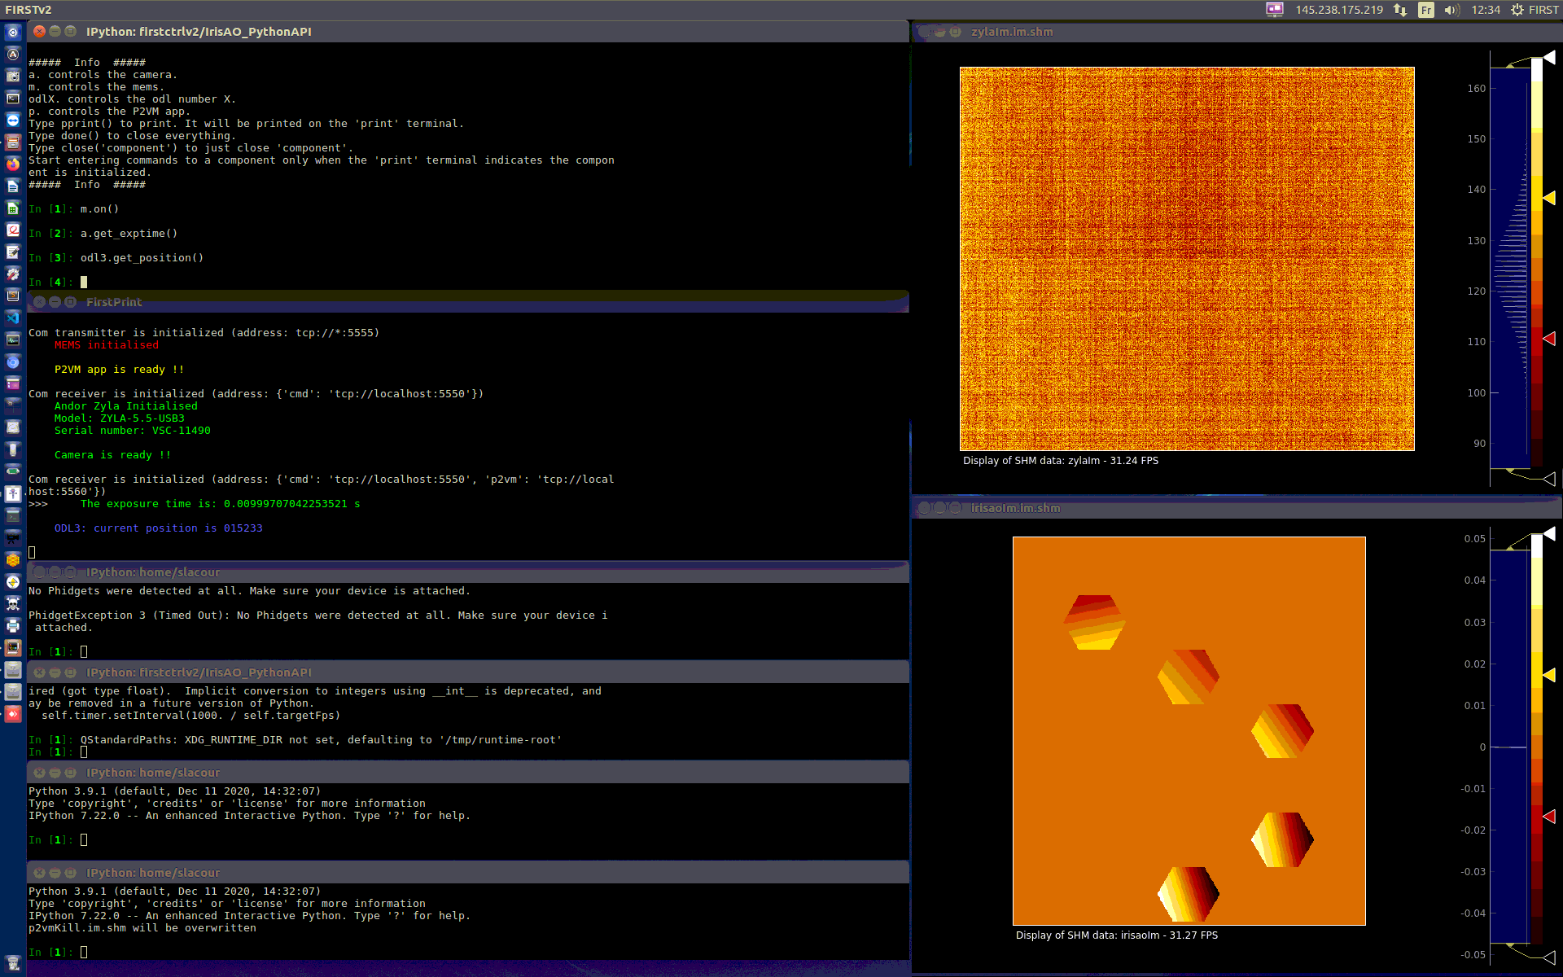
\includegraphics[angle=90,height=0.78\textheight]{Figure_Chap2/FIRSTv2_ControlSoftware_ScreenShot.png}
    \caption[Capture d'écran du logiciel de contrôle du banc de test de FIRSTv2, à Meudon.]{Capture d'écran du logiciel de contrôle du banc de test de FIRSTv2, à Meudon. À gauche, sont affichés les terminaux, de haut en bas, pour l'exécution des commandes par l'utilisateur, de l'affichage de tous les messages des différents processus et ceux qui s'ouvrent à l'exécution des programmes de la caméra, du MEMS, des ODLs et de \texttt{p2vmView.py}. En haut à droite est la fenêtre d'affichage en temps réel du flux d'images de la caméra. En bas à droite est la fenêtre d'affichage en temps réel de la carte de phase de la surface du MEMS, dont cinq segments sont commandés sur leur position qui optimise l'injection du flux dans les fibres.}
    \label{fig:SoftwareScreenShot}
\end{figure}


%%%%%%%%%%%%%%%%
\subsection{La communication serveur/client avec la librairie ZeroMQ}
\label{sec:ZMQ}

La version écrite en Python de la librairie \textit{ZeroMQ}\footnote{\url{https://github.com/zeromq/pyzmq.git}} permet de créer en parallèle des processus se comportant comme des serveurs et des clients se connectant ensemble afin de s'échanger des chaînes de caractères ou des dictionnaires (objet simple du langage Python). Cette librairie rend l'implémentation de ces processus très facile (une vingtaine de lignes de code suffisent). Il existe plusieurs types de schéma de communication et les deux que j'ai utilisés son schématisés sur la figure~\ref{fig:ZMQProtocols}. Le premier (schématisé à gauche), est le schéma \textit{request/reply} nommé \textit{REQ/REP}. Un script est écrit pour le processus serveur et un autre est écrit pour le processus client. Le principe est que le processus associé au client envoie une requête sous forme d'une chaîne de caractères à une adresse définie et se met en attente d'une réponse. Le serveur est implémenté en étant associé à cette adresse et se met dans un premier temps en attente d'une requête et dans un second temps envoie une réponse (sous forme d'une chaîne de caractères) lorsqu'il reçoit la requête, avant de se remettre en attente. Enfin, le client reçoit à son tour la réponse du serveur. Cela permet, par exemple, de mettre en place un serveur hébergeant un site internet sur lequel des utilisateurs font des requêtes de connexion. La librairie \textit{ZeroMQ} se charge d'implémenter les ports de connexion identifiés par une adresse, l'envoi des informations, la mise en attente du serveur et du client, etc de manière très simple. J'ai ainsi utilisé ce schéma de communication pour que le processus nommé \texttt{p2vmView.py} puisse se connecter successivement à chaque composant, en s'assurant que les composants sont disponibles, afin d'envoyer des commandes de contrôle et d'attendre que l'exécution de ces commandes se termine avant d'en envoyer une autre.

\begin{figure}[ht!]
    \centering
    \begin{subfigure}{0.45\textwidth}
        \centering
        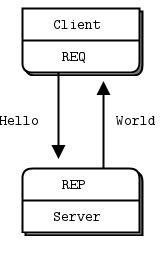
\includegraphics[width=0.5\textwidth]{Figure_Chap2/ZMQ_ReqRep_Figure.png}
    \end{subfigure}%
    \begin{subfigure}{0.45\textwidth}
        \centering
        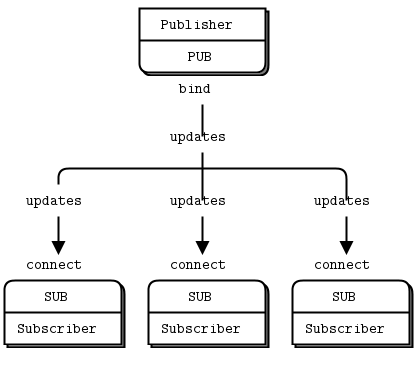
\includegraphics[width=\textwidth]{Figure_Chap2/ZMQ_PubSub_Figure.png}
    \end{subfigure}
    \caption[Schémas des processus de communication request/reply et publisher/subscriber de la librairie ZeroMQ.]{Schémas des processus de communication request/reply (à gauche) et publisher/subscriber (à droite) implémenté par la librairie ZeroMQ. Crédit : \textit{ZeroMQ}.}
    \label{fig:ZMQProtocols}
\end{figure}

Le deuxième schéma de communication (à droite sur la figure~\ref{fig:ZMQProtocols}) que j'ai utilisé est le \textit{publisher/subscriber} nommé \textit{PUB/SUB}. Il s'agit d'implémenter un publieur qui peut envoyer à n'importe quel moment une chaîne de caractère et des abonnés (\textit{subscriber}) qui se connectent au publieur et reçoivent la chaîne de caractère. Je me suis servis de ce schéma de communication pour l'envoi des commandes par l'utilisateur (le terminal de commande utilisateur est le publieur) aux processus associés aux composants (qui sont les abonnés). Une partie du message envoyé contient un caractère d'identification lu par tous les abonnés afin de savoir quel composant doit exécuter la commande en question. J'ai aussi implémenté ce système pour afficher tous les messages sur un unique terminal (\texttt{FirstPrint.py}) dont le processus s'abonne à tous les processus des composants qui sont des publieurs. Chaque script peut en fait implémenter des processus publieur, abonné, serveur et client en parallèle (via la technique de \textit{Threading}\footnote{\url{https://fr.wikipedia.org/wiki/Thread_(informatique)}}).


%%%%%%%%%%%%%%%%
\subsection{La gestion des flux de données avec la librairie pyMilk}
\label{sec:SHM}
% Vincent Déo : MILK est tout a fait concu pour le streaming à haute fréquence. La limite est imposée par la vitesse à laquelle la mémoire arrive à copier les données encore et encore, plus quelques glitch quand on dépasse les 10kHz. On fait régulièrement des acquisitions à 10kHz sur SCExAO. On a déjà fait tourner des SHMs à 35kHz expérimentalement. C'est moins stable mais c'est possible!

% Vincent Déo (mail) : 
% Si j'étais toi, je schématiserai un peu plus en clarifiant ce qu'est exactement le contenu d'un stream:
% - Des données, accessibles en écriture par tous les processus sur la machine
% - Des métadonnées (compteur, temps d'accès et d'écriture, compteurs en écriture, ID des processus qui consultent la SHM), accessibles idem
% - Des sémaphores, qui permettent une synchronisation à sens unique entre le process qui écrit et les process qui lisent.
% On peut s'en servir pour des pipelines temps réel, et les sémaphore permettent 1/ d'attendre passivement la prochaine trame, donc d'économiser des ressources; et 2/ de démarrer instantanément lorsque le sémaphore est posté, donc d'économiser du temps.
% On peut aussi s'en servir juste comme de la mémoire partagée non-synchronisée, et c'est juste pratique.

% Enfin, si on imaginait que tu voudrais moduler tes franges à vitesse kHz+, ce n'est pas seulement l'utilisation de sémaphores qui permet la synchronisation, c'est:
% - les sémaphores, plus
% - L'utilisation d'un OS temps-réel, dans le quel une action donnée prend une durée (quasi) déterministe
% - La calibration propre de la latence du système pour "aligner" temporellement les trames sur le DM et les durées d'exposition de la caméra.

% La combinaison de ces trois éléments permet, in fine, d'utiliser l'horloge interne d'une caméra comme primitive de synchronisation pour tout où partie d'une manip, à une précision de quelques microsecondes RMS, là où par le passé il fallait utiliser des triggers en hardware dès lors qu'il fallait des précisions sub-ms.

La librairie écrite en Python \ac{pyMILK}\footnote{\url{https://github.com/milk-org/pyMilk.git}} permet un interfaçage simple (moins d'une dizaine de lignes de codes suffisent) entre les scripts du logiciel écrits en Python et la librairie \ac{MILK}\footnote{\url{https://github.com/milk-org/milk-package.git}} écrite en langage C et utilisée dans le contrôle du banc \ac{SCExAO} \citep{guyon2020}. Elle permet d'allouer un espace mémoire partagée sur la \ac{RAM} de l'ordinateur (nommé \ac{SHM}) pour le stockage, la lecture, la réduction et l'analyse de données, en temps réel et à haute fréquence.

Ce flux de données se compose :
\begin{itemize}
    \item des données stockées dans l'espace de mémoire partagée \ac{SHM}, qui sont accessibles par n'importe quel processus sur l'ordinateur;
    \item des méta-données composées de compteurs du nombre de données, du temps d'accès et d'écriture des données, des numéros d'identification des processus qui consultent la \ac{SHM} et sont aussi accessibles par les autres processus;
    \item des sémaphores\footnote{\url{https://fr.wikipedia.org/wiki/S\%C3\%A9maphore_(informatique)}} qui permettent la synchronisation entre le processus qui écrit et celui qui lit.
\end{itemize}

Ces sémaphores permettent aux processus qui lisent les \ac{SHM}s de se mettre en attente de manière passive jusqu'à ce qu'une nouvelle donnée est écrite et, lorsqu'elle est écrite, de reprendre le cours de l'exécution. Cette pratique permet ainsi d'économiser des ressources et du temps de calcul. De plus, en les utilisant en combinaison avec la connaissance de la durée (qui est en fait quasi-déterministe) que prend une action sur le système d'exploitation de l'ordinateur et avec l'étalonnage de la latence de ce système, il est possible de synchroniser plusieurs éléments logiciels ou matériels (comme un miroir déformable) à l'horloge interne d'une caméra à des fréquences de plus de $1 \,$kHz et avec une précision de quelques $\upmu$s rms. C'est ce qui est implémenté pour faire fonctionner l'optique adaptative sur \ac{SCExAO} et il a été mesuré des fréquences de fonctionnement de la caméra et du miroir déformable en synchronisation jusqu'à $\sim 10 \,$kHz et plus. Un ordinateur doté d'une puissance de calcul suffisante pour faire une telle synchronisation a récemment été acheté pour le projet \ac{FIRST} sur \ac{SCExAO}. Lors de futurs développements, il s'agira de mettre en place la modulation des franges à une fréquence de l'ordre du kHz, permettant la mesure des interférogrammes sans que les franges subissent les perturbations de phase de l'environnement du banc et des résidus de l'optique adaptative.

Dans le logiciel de contrôle du banc \ac{FIRSTv2}, cette librairie est cruciale pour échanger des données entre différents processus de manière fluide et rapide. En effet, par exemple, pour la modulation des franges, une \ac{SHM} (nommée \og mems modulation \fg~sur la figure~\ref{fig:SoftwareArchitecture} du bas) est créée par le processus de la caméra. Celle-ci contient un nombre qui est incrémenté par la caméra après l'acquisition de chaque image et le processus associé au \ac{MEMS} change les segments de positions en conséquence. Cela permet ainsi de parfaitement synchroniser la caméra et le \ac{MEMS} pour la modulation rapide des franges (typiquement à $20 \,$Hz mais pouvant aller jusqu'à la centaine de Hz). Mais encore, ce principe est utilisé pour l'optimisation de l'injection du flux dans les fibres par le logiciel. En effet, le processus associé au \ac{MEMS} se connecte à la mémoire partagée des images de la caméra (nommée \og live feed \fg) et à chaque fois qu'un segment est déplacé en tip-tilt, une image de la caméra est récupérée pour estimer l'intensité du flux des sorties afin de construire les cartes de transmission des fibres optiques (pour plus de détails voir la section~\ref{sec:OptiInj}). La même chose est implémentée sur le programme associé aux \ac{ODL}s pour la recherche des franges.

La librairie dispose aussi d'un module de visualisation de données qui passent par les \ac{SHM}s, qui est utilisé par le logiciel de \ac{FIRSTv2} pour visualiser en temps réel le flux d'images de la caméra ainsi que la carte de phase instantanée de la surface du \ac{MEMS}. Le module ouvre une fenêtre sur l'écran de l'ordinateur, dans laquelle la dernière image est affichée. Ce sont les deux fenêtres sur la droite de la capture d'écran présentée sur la figure~\ref{fig:SoftwareScreenShot}.


%%%%%%%%%%%%%%%%%%%%%%%%%%%%%%%%
\section{La configuration des bases}
\label{sec:BaseConfig}

Les sous-pupilles choisies sur le banc de test lors de l'acquisition de toutes les données qui sont présentées et analysées par la suite, sont représentées sur la figure~\ref{fig:SegUVSimuleA} à l'aide de la carte des segments du \ac{MEMS}. Les segments considérés pour former les bases sont en orange et le plan UV correspondant est tracé sur la figure~\ref{fig:SegUVSimuleB}. J'ai choisi ces sous-pupilles pour échantillonner au mieux le plan UV dans la direction horizontale, qui correspond à la direction du système simulé. En effet, comme l'indique l'équation~\ref{eq:PhaseBinaireCentree} les signaux de phases dépendent de la projection des bases sur l'orientation du système protoplanétaire observé et étant orienté horizontalement par rapport à la carte des segments (dans la même direction que la base $37-33$ par exemple), il n'y a bien que trois signaux d'intensités différentes qui peuvent être mesurés. Ces trois types de signaux proviennent des groupes de bases suivants :
\begin{itemize}
    \item les bases qui sont orthogonales à la source et qui donnent un signal nul e.g. les bases $7-26$ et $15-28$;
    \item les bases qui s'étendent sur un segment et demi projeté e.g. $37-7$, $37-26$, $7-15$, $7-28$, $26-15$ et $26-28$, de longueur égale à $1,05 \,$mm 2,1;
    \item et les bases qui s'étendent sur trois segments projetés e.g. $37-15$ et $37-28$, de longueur égale à $2,10 \,$mm, équivalentes aux plus grandes bases sur le télescope Subaru de longueur $6,86 \,$m.
\end{itemize}

\begin{figure}[ht!]
    \centering
    \begin{subfigure}{0.39\textwidth}
        \centering
        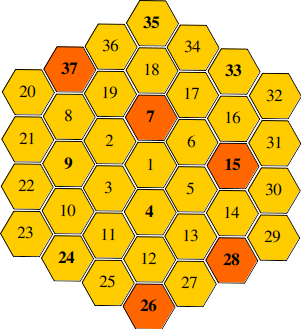
\includegraphics[width=\textwidth]{Figure_Chap2/BaselineMap_37_7_26_15_28.png}
        \caption{Configuration des sous-pupilles choisies (en orange) dans le plan pupille sur la carte des segments du MEMS.}
        \label{fig:SegUVSimuleA}
    \end{subfigure}\hfill
    \begin{subfigure}{0.59\textwidth}
        \centering
        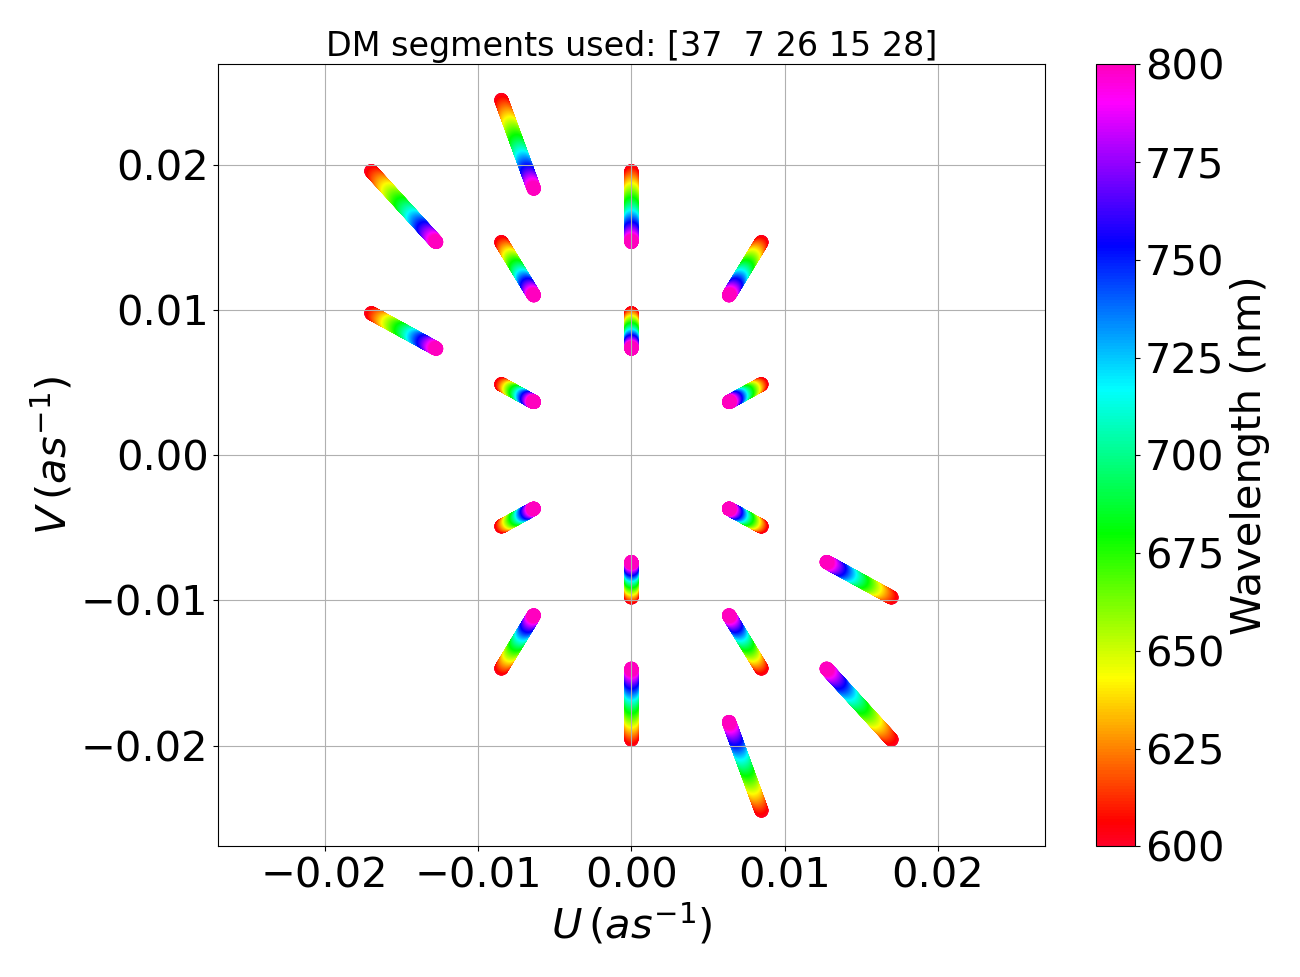
\includegraphics[width=\textwidth]{Figure_Chap2/UVplane_Meudon_37_7_26_15_28.png}
        \caption{La répartition des bases choisies représentée dans l'espace de Fourier, appelée aussi la couverture du plan UV des fréquences spatiales. Les couleurs représentent la longueur d'onde.}
        \label{fig:SegUVSimuleB}
    \end{subfigure}
    \caption[Configuration des sous-pupilles et couverture du plan UV du banc de test de FIRSTv2.]{Configuration des sous-pupilles et couverture du plan UV du banc de test de FIRSTv2.}
    \label{fig:SegUVSimule}
\end{figure}

Historiquement, sur les instruments implémentant la technique de masquage de pupille, les bases sont choisies non-redondantes pour éviter le brouillage des franges (voir la section~\ref{sec:PupilMasking}). Ici, les bases peuvent être choisies redondantes car on utilise le principe de réarrangement de pupille ce qui empêche les interférogrammes provenant de chaque base de se superposer sur le détecteur. Il n'y a donc pas de risque que les franges se brouillent. Cependant, lorsque l'instrument sera utilisé sur une cible astrophysique, les bases seront choisies de manière la plus non-redondante possible pour que la couverture du plan UV soit maximisée et homogène dans le but de sonder le plus possible de fréquences spatiales différentes. C'est ce que j'ai fait ici et les bases $37-7$ et $7-15$ sont les seules à être redondantes. Finalement, seulement deux fréquences spatiales sont sondées (correspondant à deux longueurs de base projetée différentes) car le montage du banc n'en permet pas plus du fait que seul les segments $37 - 9 - 24 - 35 - 7 - 4 - 26 - 33 - 15 - 28$ peuvent être utilisés (pour plus de détails, voir la section~\ref{sec:FiberInjection}). Enfin, on note que la couverture du plan UV présentée sur la figure~\ref{fig:SegUVSimuleB} est calculée pour toute la bande spectrale transmise par l'instrument, mais que lors de la détection de protoplanètes grâce à leur raie d'émission \ha, la couverture de ce plan UV effective est alors réduite aux canaux spectraux correspondant.


%%%%%%%%%%%%%%%%%%%%%%%%%%%%%%%%
\section{Conclusion}

Ce chapitre nous a permis de présenter les avancées de l'intégration de la technologie d'optique intégrée sur le banc de test \ac{FIRSTv2} tout en le présentant dans sa globalité. Une partie de mon travail de thèse, qui est présentée dans ce chapitre, est la caractérisation en transmission, \textit{cross-talk}, contraste interférométrique et polarisation de deux puces photoniques utilisant deux concepts de recombinaison différentes : couplage directionnel et jonction $Y$. La transmission de la première est estimée à $30\%$ et celle de la deuxième à $13\%$, ce qui nous a conduit à décider de les intégrer sur le banc \ac{SCExAO} pour la première lumière de \ac{FIRSTv2} (présentée dans le chapitre~\ref{sec:FIRSTv2Subaru}). Ainsi, de nouvelles puces sont actuellement en cours de développement à l'\ac{IPAG} pour améliorer ces performances, dans l'objectif d'atteindre une transmission d'au moins $75\%$.

Dans le même but d'augmenter la transmission de l'instrument, il est envisagé de retirer les lignes à retard car leur transmission s'avère être trop faible. Pour cela, on pourra concevoir des fibres de compensation qui égaliseraient tous les chemins optiques et/ou opter pour une nouvelle technologie de puce photonique telle qu'un composant 3D ou une lanterne photonique qui permettraient aussi de se passer du toron de fibres en plus des \ac{ODL}s.

Une autre partie de mon travail est la restructuration et la continuation du développement du logiciel de contrôle du banc de test. Cela a permis d'améliorer sa rapidité d'exécution, sa modularité ainsi que d'ajouter des processus d'acquisitions automatiques de données interférométriques. Je l'ai ainsi déployé sur l'ordinateur de contrôle de \ac{FIRSTv1} au télescope Subaru et il a été utilisé lors de quelques nuits d'observations avec succès.


%%%%%%%%%%%%%%%%%%%%%%%%%%%%%%%%
\clearpage
\section*{Conférence SPIE}
\label{sec:SPIEproceeding}
\phantomsection
\addcontentsline{toc}{section}{Conférence SPIE}

\clearpage

\includepdf[pages=-, pagecommand={}, offset=-10 -20, templatesize={0.8\textwidth}{0.8\textheight}]{Paper/Barjot2020_SPIE_FIRSTv2LabPhotonicCharacterization.pdf}



\clearpage
%%%%%%%%%%%%%%%%%%%%%%%%%%%%%%%%%%%%%%%%%%%%%%%%%%%%%%%%%%%%%%%%
\section{Le traitement des données FIRSTv2}
\setcounter{figure}{0}
\setcounter{table}{0}

L'objectif de cette section est de présenter les données de \ac{FIRSTv2}, depuis leur acquisition et les procédures mises en place dans ce cadre jusqu'à leur traitement. Il s'agit aussi de présenter le formalisme mathématique de ce traitement de données afin d'établir les observables que l'on infère des données de \ac{FIRSTv2}.


%%%%%%%%%%%%%%%%%%%%%%%%%%%%%%%%
\subsection{L'acquisition des données}

%%%%%%%%%%%%%%%%
\subsubsection{Morphologie des images}

%%%%%%%%
\threesubsection{Étalonnage du détecteur}
\label{sec:CameraDark}

Comme décrit dans la section~\ref{sec:InstruCamera}, les images sont d'une taille de $2160 \,$px de hauteur par $2559 \,$px de largeur. La figure~\ref{fig:DarkFull} montre, à gauche, une image sans frange prise avec un temps d'exposition de $100 \,$ms et à droite la médiane d'un cube de $100$ images sans frange au même temps d'exposition. Ces images permettent de caractériser le courant d'obscurité et le bruit du détecteur de la caméra. 

Un tel cube sans frange est systématiquement acquis à chaque prise de données interférométriques. Le début du traitement des images consiste au calcul de la médiane de ce cube sans frange qui est ensuite soustraite aux images interférométriques diminuant ainsi le biais du détecteur et les structures fixes mentionnées dans le paragraphe précédent, présents sur toutes les données. Afin d'effectuer cette soustraction sans se soucier d'une possible dépendance non linéaire du courant d'obscurité du détecteur en fonction du temps d'exposition, ce dernier est choisi identique pour les deux types de données (sans et avec franges).

\begin{figure}[ht!]
    \begin{subfigure}{.5\textwidth}
        \centering
        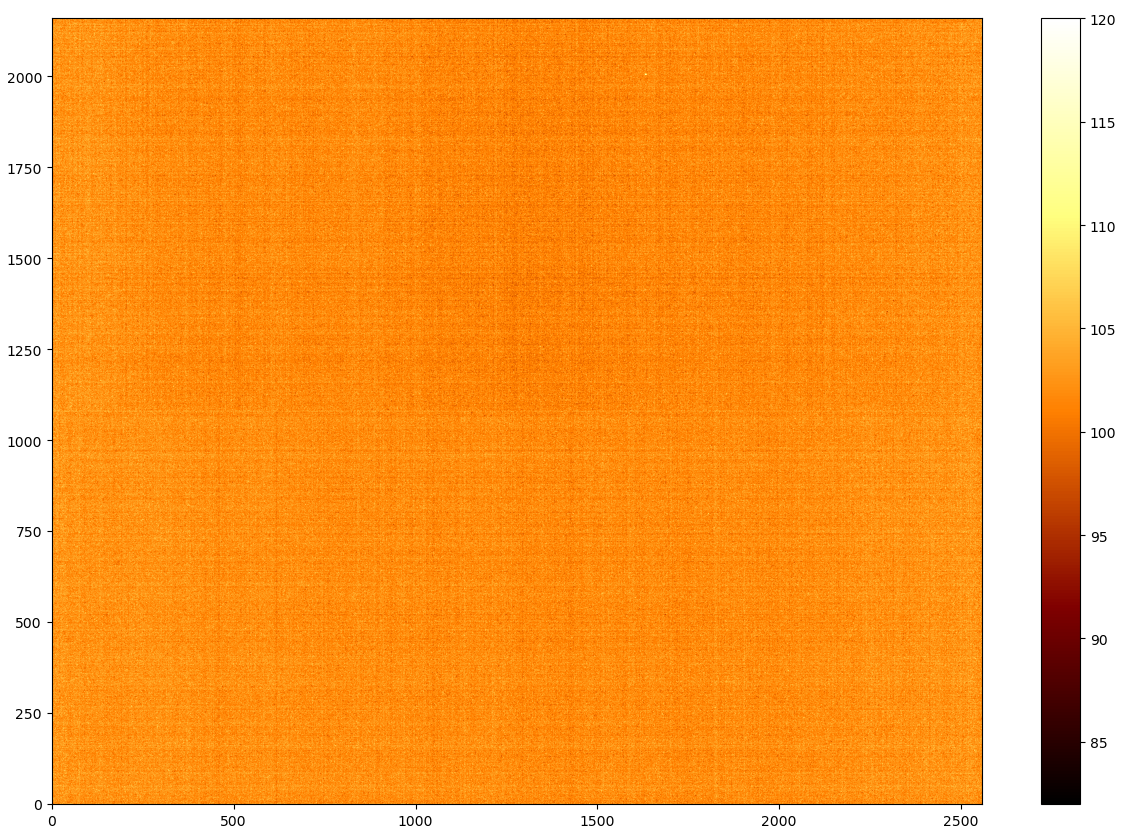
\includegraphics[width=0.9\textwidth]{Figure_Chap3/20220705_DarkFullImage_100ms_24C_Im0.png}
    \end{subfigure}%
    \begin{subfigure}{.5\textwidth}
        \centering
        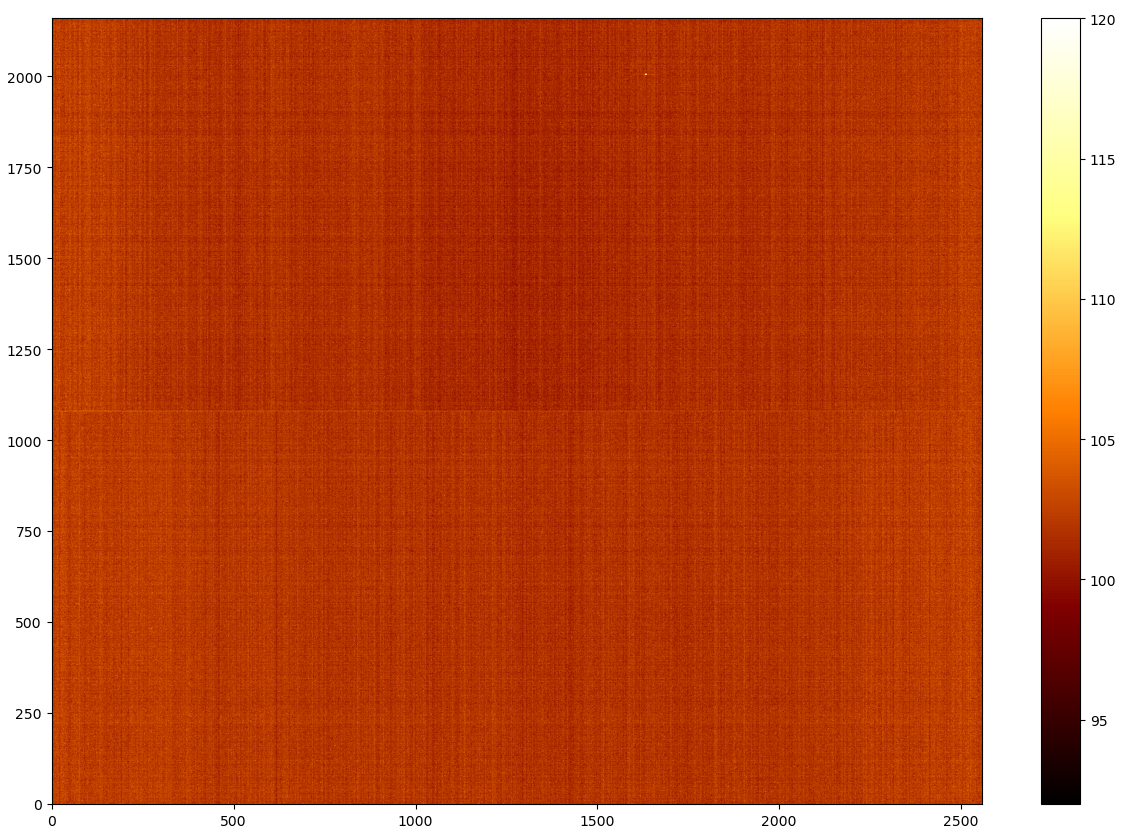
\includegraphics[width=0.9\textwidth]{Figure_Chap3/20220705_DarkFullImage_100ms_24C_median.png}
    \end{subfigure}
    \caption[Images du courant d'obscurité de la caméra de FIRSTv2.]{A gauche une image de la caméra non illuminée et à droite la médiane de $100$ de ces images, pour le même temps d'exposition de $100 \,$ms. Les valeurs des pixels données sur les échelles sont en \ac{ADU}.}
    \label{fig:DarkFull}
\end{figure}


%%%%%%%%
\threesubsection{Les images interférométriques}

Les images acquises avec la caméra sont rognées pour cadrer les sorties de la puce d'optique intégrée. La puce $Y$ a $10$ sorties et la puce $X$ a $20$ sorties, qui peuvent être dédoublées lorsqu'elles sont imagées par la caméra quand le prisme de wollaston est installé sur le chemin optique. Les différentes configurations possibles peuvent donc amener à avoir $10$, $20$ ou $40$ sorties à cadrer. Ce rognage dépend aussi de la bande spectrale de la source utilisée (changeant la largeur de l'image) et est choisi de façon à encadrer celle-ci le plus largement possible. Pour chaque montage sur le banc toutes les images (sans franges, \textit{flats} ou interférométriques) sont acquises avec le même rognage. La figure~\ref{fig:FringeCrop} présente deux images obtenues avec la caméra avec les sorties de la puce $X$ imagées sans que le prisme de wollaston soit installé ($20$ sorties sont donc visibles). La \sk est la source utilisée et les images ont alors une taille de $320 \,$px par $1800 \,$px ($1800$ canaux spectraux). En haut est montrée la médiane de $300$ images sans frange, qui est soustraite à une image avec des franges dont le résultat est montré en bas, pour un temps d'exposition de $50 \,$ms.

\begin{figure}[ht!]
    \centering
    \begin{subfigure}{0.9\textwidth}
        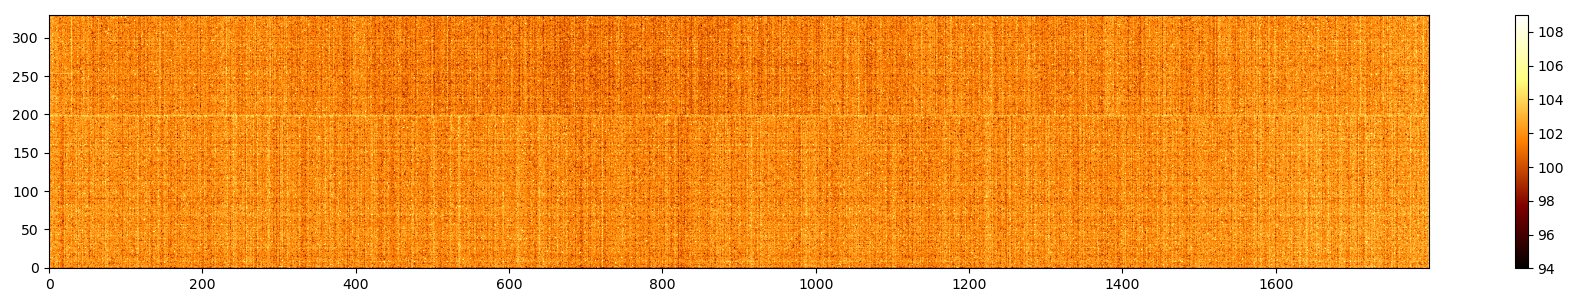
\includegraphics[width=\textwidth]{Figure_Chap3/20220614_P2VM_Dark1_50ms_median300.png}
    \end{subfigure}
    \begin{subfigure}{0.9\textwidth}
        \includegraphics[width=\textwidth]{Figure_Chap3/20220614_P2VM_FullOn_001_50ms_Im0_SubDark.png}
    \end{subfigure}
    \caption[Image interférométrique obtenues sur FIRSTv2.]{En haut la médiane de $300$ images de la caméra sans franges et en bas une image avec des franges, avec la source \sk. Les deux images ont été acquises avec un temps d'exposition de $50 \,$ms et le même rognage induisant une taille d'image de $320 \, px$ de hauteur par $1800 \, px$ de largeur.}
    \label{fig:FringeCrop}
\end{figure}

Les lignes à retard sont au voisinage de leur position d'\ac{OPD} nulle, ce qui se traduit par la présence de franges sur l'image du bas. Il y a donc pour chacun des $1800$ canaux spectraux, un point de mesure du flux interférométrique pour chacune des $20$ sorties, correspondant à une valeur d'\ac{OPD}. L'objectif est alors de reconstruire les $20$ figures d'interférences par la mesure du flux des $20$ sorties pour au moins $4$ valeurs d'\ac{OPD}s par base. A cette fin, nous avons besoin de bouger en piston les cinq segments du \ac{MEMS} qui illuminent les cinq entrées de la puce selon la méthode décrite dans la section~\ref{sec:Modulation}.


%%%%%%%%%%%%%%%%
\subsubsection{Étalonnage spectral}
\label{sec:EtalonnageSpectral}

Ici on souhaite associer à chaque pixel une valeur de longueur d'onde. Pour cela, j'utilise une lampe à vapeur de néon (Avalight-CAL-NEON par Avantes, avec sortie fibrée FC-PC). Le spectre d'émission de la vapeur de Néon est connu et présente de nombreuses raies sur la bande spectrale détectée par \ac{FIRSTv2}. La figure~\ref{fig:NeonReference} montre deux spectres de référence de l'émission de la vapeur de Néon, que j'ai utilisés pour les étalonnages spectraux durant ma thèse, celui de gauche étant un spectre que j'ai trouvé sur le site internet Astrosurf\footnote{\url{http://www.astrosurf.com/buil/us/spe2/calib2/neon1.gif}} et le deuxième étant celui mesuré par \ac{FIRSTv1} pendant la thèse d'Elsa Huby. Les deux spectres présentent des pics d'émission à des longueurs d'onde différentes et permettent donc d'identifier toutes les raies mesurées par \ac{FIRSTv2}.

\begin{figure}[ht!]
    \centering
    \begin{subfigure}{0.5\textwidth}
        \includegraphics[width=\textwidth]{Figure_Chap3/Neon_SpectrumReference_Astrosurf.png}
    \end{subfigure}%
    \begin{subfigure}{0.5\textwidth}
        \includegraphics[width=\textwidth]{Figure_Chap3/Neon_SpectrumReference_ThesisEHuby.png}
    \end{subfigure}
    \caption[Spectres de référence d'émission du Néon utilisés pour l'étalonnage spectral de \ac{FIRSTv2}.]{Spectres de références d'émission du Néon utilisés pour l'étalonnage spectral de \ac{FIRSTv2}. À gauche est un spectre trouvé sur le site Astrosurf, présentant l'intensité des raies d'émissions du Néon (axe des ordonnées) en fonction de la longueur d'onde en Angstrom (axe des abscisses). À droite est le spectre tel que mesuré par FIRSTv1 pendant la thèse d'Elsa Huby traçant l'intensité des raies d'émission du Néon (axe des ordonnées) en fonction des pixels (axe des abscisses) de la caméra utilisée. Sur les deux spectres la longueur d'onde des pics est notée sur le graphique au-dessus de chaque pic.}
    \label{fig:NeonReference}
\end{figure}

La méthodologie utilisée pour conduire l'étalonnage spectral est la suivante :

\begin{enumerate}
    \item cinq séquences d'images sont acquises en illuminant successivement les cinq entrées de la puce avec la lampe néon;
    \item la somme des cinq moyennes de ces séquences est calculée pour donner une unique image avec toutes les sorties de la puce;
    \item une première étape d'identification des raies est effectuée avec une fonction de détection de pics pour chaque sortie;
    \item ensuite ces positions des pics sont passées en paramètres d'une fonction d'ajustement gaussien, afin de calculer finement la position centrale des pics et permettre leur identification en longueur d'onde;
    \item enfin, les longueurs d'ondes des pics sont ajustées aux positions des pics à l'aide d'une fonction polynomiale de degré 4.
\end{enumerate}

La figure~\ref{fig:NeonSpecCal} du haut montre l'image résultante de l'étape \textit{1.} en échelle logarithmique, la courbe du milieu montre l'identification précise des pics à l'issue de l'étape \textit{4.} sur le spectre d'émission de la lampe néon mesurée sur la sortie 1 de \ac{FIRSTv2} et la courbe du bas présente l'ajustement polynomial de l'étape \textit{5.}, pour la sortie 1 également. L'équation du polynôme trouvée par ajustement est montrée dans la légende et on remarque que la répartition des longueurs d'ondes sur les pixels du détecteur suit une loi affine. Cet ajustement a l'avantage de permettre l'extrapolation du modèle sur l'entièreté du détecteur, ce qui est utile lorsqu'on utilise la source \sk qui a une plus large bande que la lampe néon. Finalement, nous disposons d'autant d'équations de cet ajustement qu'il y a de sorties imagées sur la caméra et elles seront utilisées dans la suite du traitement de données, à chaque calcul en fonction de la longueur d'onde (notamment sur les phases) ou à chaque fois que des courbes seront tracées en fonction de la longueur d'onde. Enfin, il est indiqué dans le titre du graphique du milieu la résolution spectrale mesurée lors de l'étalonnage, qui est ici de $3184$ à $651 \,$nm. Elle a été mesurée sur toutes les sorties en moyenne à $3254$ avec un écart-type de $127$.

\begin{figure}[ht!]
    \centering
    \begin{subfigure}{0.8\textwidth}
        \includegraphics[width=\textwidth]{Figure_Chap3/20210722_5TC_Y_5InputsSum_Neon.png}
    \end{subfigure}
    \begin{subfigure}{0.8\textwidth}
        \includegraphics[width=\textwidth]{Figure_Chap3/20210722_5TC_PY_SpectralCalFlux01_Neon.png}
    \end{subfigure}
    \begin{subfigure}{0.8\textwidth}
        \includegraphics[width=\textwidth]{Figure_Chap3/20210722_5TC_Y_SpectralCalFitFort01_Neon_Manuscript.png}
    \end{subfigure}
    \caption[Résultat de l'étalonnage spectrale de FIRSTv2 avec une lampe spectrale au néon.]{Étalonnage spectral de FIRSTv2 à l'aide d'une lampe spectrale au néon. En haut : image de la caméra avec le spectre de la lampe néon sur chaque sortie. Au milieu : identification des pics du spectre du néon sur les pixels de la caméra pour la sortie 1. En bas : les longueurs d'onde du néon en fonction des positions des pics sur la caméra ainsi que l'ajustement polynomial associé, de la sortie 1.}
    \label{fig:NeonSpecCal}
\end{figure}


%%%%%%%%%%%%%%%%
\subsubsection{La modulation des franges}
\label{sec:Modulation}

L'acquisition des données interférométriques s'effectue en modulant les franges à l'aide des \ac{MEMS}. Ces derniers sont synchronisés avec la caméra de telle sorte que chaque image d'une séquence contienne les franges pour une valeur différente d'\ac{OPD}. La figure~\ref{fig:FringeSamplingABCD} montre la méthode ABCD utilisée pour mesurer une frange, représentée sur le graphique par une période de la fonction sinusoïdale ($2 \pi$). Cette période est divisée en $8$ et un déphasage de $\frac{3}{8} 2 \pi \,$rad, $\frac{-1}{8} 2 \pi \,$rad, $\frac{1}{8} 2 \pi \,$rad et $\frac{-3}{8} 2 \pi \,$rad est appliqué sur chaque base pour mesurer quatre points de la frange. Pour cela on applique quatre valeurs de piston sur deux segments du \ac{MEMS}, définis comme multiples de la longueur d'onde, prise égale à $750 \,$nm : $\frac{3}{8} \frac{0.750}{4} \,$\um, $\frac{-1}{8} \frac{0.750}{4} \,$\um, $\frac{1}{8} \frac{0.750}{4} \,$\um~et $\frac{-3}{8} \frac{0.750}{4} \,$\um. Comme ce sont les valeurs mises en consignes des segments, deux facteurs $1/2$ sont présents pour prendre en compte que (1) l'\ac{OPD} effective est la somme des déplacements de $2$ segments ainsi que (2) la lumière parcourt deux fois la même distance en étant réfléchie sur les segments.

\begin{figure}[htp!]
    \centering
    \includegraphics[width=0.8\textwidth]{Figure_Chap3/Fringe_Sampling_ABCD.png}
    \caption[Méthode ABCD d'échantillonnage d'une frange.]{Méthode ABCD d'échantillonnage d'une frange. Ici la frange est représentée par une période de la fonction sinusoïdale ($2 \pi$) et pour l'échantillonner, les quatre valeurs de déphasage égales à $\frac{3}{8} 2 \pi \,$rad, $\frac{-1}{8} 2 \pi \,$rad, $\frac{1}{8} 2 \pi \,$rad et $\frac{-3}{8} 2 \pi \,$rad sont appliquées par les segments du MEMS.}
    \label{fig:FringeSamplingABCD}
\end{figure}

Une première approche est d'appliquer quatre valeurs de pistons, successivement, par paire de segments, pour effectuer les quatre points de mesures par base, ce qui constitue une séquence de modulation de $20$ points de mesure. La figure~\ref{fig:ModSeq20} du haut montre les valeurs de piston (en couleur) appliquées aux segments (selon l'axe vertical) en fonction des étapes de modulation (selon l'axe horizontal). La figure du bas montre les valeurs effectives d'\ac{OPD}s tout au long de la séquence de modulation pour les dix bases. On remarque qu'il y a deux types de quadruplets de valeurs d'\ac{OPD}s dans cette séquence. Le premier type (aux valeurs les plus élevées sur la figure) contient les valeurs précédemment définies ($\frac{3}{8} \frac{0.750}{4} \,$\um, $\frac{-1}{8} \frac{0.750}{4} \,$\um, $\frac{1}{8} \frac{0.750}{4} \,$\um~et $\frac{-3}{8} \frac{0.750}{4} \,$\um) car elles sont obtenues en déplaçant deux segments et sont appliquées sur les bases $1-2$, $2-3$, $3-4$, $4-5$ et $1-5$. Le deuxième type contient quatre valeurs dont les amplitudes sont moitié moindres que celles du premier type ($\frac{3}{8} \frac{0.750}{8} \,$\um, $\frac{-1}{8} \frac{0.750}{8} \,$\um, $\frac{1}{8} \frac{0.750}{8} \,$\um~et $\frac{-3}{8} \frac{0.750}{8} \,$\um) car elles sont obtenues avec un des deux segments immobile et sont appliquées sur les bases $1-3$, $1-4$, $2-4$, $2-5$ et $3-5$. Par conséquent, la moitié des bases sont modulées sur une OPD deux fois trop petite ce qui ne permet pas un bon échantillonnage des franges et empêchant le code de traitement de données de converger.

\begin{figure}[ht!]
    \centering
    \begin{subfigure}{0.8\textwidth}
        \centering
        \includegraphics[width=\textwidth]{Figure_Chap3/20210503_MEMSModulationSequence_Standard_step20.png}
    \end{subfigure}
    \begin{subfigure}{0.8\textwidth}
        \centering
        \includegraphics[width=\textwidth]{Figure_Chap3/20210503_MEMSModulationSequence_Standard_step20_DiffBase.png}
    \end{subfigure}
    \caption[Séquence basique de modulation des MEMS à 20 pas pour échantillonner les franges sur FIRSTv2.]{En haut la séquence des pistons (en $\upmu$m) appliqués aux cinq segments du MEMS qui illuminent les entrées de la puce. En bas les valeurs d'OPDs (en $\upmu$m) induites sur les dix bases en application de cette séquence de modulation. Les couleurs sont les valeurs appliquées, les axes horizontaux sont les étapes de la séquence et les axes verticaux sont les segments et les bases, respectivement, pour la figure du haut et du bas.}
    \label{fig:ModSeq20}
\end{figure}

Une deuxième approche est de moduler plusieurs bases en même temps et non une seule à la fois comme précédemment. Il faut alors s'assurer que chaque base soit modulée au moins une fois par le bon quadruplet de pistons durant la séquence de modulation. La figure~\ref{fig:ModSeq12} montre un exemple d'une telle séquence. De même que sur la figure~\ref{fig:ModSeq20}, en haut est présentée la séquence des pistons appliqués aux segments. Sur les quatre premiers pas, tous les segments sont modulés, la condition étant que la moitié des segments soient modulés avec des valeurs opposées à l'autre moitié (ici trois segments sont modulés de la même façon et deux sont modulés avec la valeur opposée). A partir de la figure du bas on peut voir les valeurs d'\ac{OPD}s induites sur les bases pour ces quatre premières étapes, nous permettant de définir les bases sur lesquelles appliquer le quadruplet pour les étapes suivantes. Ici seules les bases $1-3$, $1-5$, $2-4$ et $3-5$ ne sont pas modulées et doivent donc l'être par la suite. Ces quatre bases ne pouvant pas être modulées sur le bon quadruplet d'\ac{OPD}s en même temps, il faut alors les moduler sur huit étapes de plus. La séquence résultante est ainsi composée de $12$ étapes. Cette nouvelle séquence a les deux atouts suivants :

\begin{enumerate}
    \item elle permet la modulation des franges sur les quatre points d'échantillonnage, à la bonne amplitude;
    \item elle a aussi le bon goût d'être plus courte ($12$ étapes contre $20$) ce qui permet de réduire l'influence des perturbations atmosphériques (lorsque l'instrument fait des mesures sur ciel) et/ou présents sur le banc (mouvements d'air, vibrations, etc.).
\end{enumerate}

On note que la longueur de cette séquence peut être divisée par deux lorsqu'on utilise la puce $X$. En effet, avec cette puce, chaque image contient deux mesures de frange, déphasées de $\pi \,$rad (voir la section~\ref{sec:ChipConcept}). Mais au cours de cette thèse, cette propriété de la puce $X$ n'a pas été utilisée et les interférogrammes mesurés avec cette puce ont été exploités séparément car il serait nécessaire d'écrire une partie en plus dans le programme de réduction de données et de faire de nouveaux tests pour vérifier la valeur du déphasage entre les couples de sorties. La même séquence de modulation a ainsi été utilisée pour les deux puces.

\begin{figure}[ht!]
    \centering
    \begin{subfigure}{0.8\textwidth}
        \centering
        \includegraphics[width=\textwidth]{Figure_Chap3/20220826_MEMSModulationSequence_GoodSampling_step12.png}
    \end{subfigure}
    \begin{subfigure}{0.8\textwidth}
        \centering
        \includegraphics[width=\textwidth]{Figure_Chap3/20220826_MEMSModulationSequence_GoodSampling_step12_DiffBase.png}
    \end{subfigure}
    \caption[Séquence optimisée de modulation des MEMS à 12 pas pour échantillonner les franges sur FIRSTv2.]{En haut la séquence optimisée des pistons (en $\upmu$m) appliqués aux cinq segments du MEMS qui illuminent les entrées de la puce. En bas les valeurs d'OPDs (en $\upmu$m) induites sur les dix bases en application de cette séquence de modulation. Les couleurs sont les valeurs appliquées, les axes horizontaux sont les étapes de la séquence et les axes verticaux sont les segments et les bases, respectivement, pour la figure du haut et du bas.}
    \label{fig:ModSeq12}
\end{figure}


%%%%%%%%%%%%%%%%%%%%%%%%%%%%%%%%
\subsection{Étalonnage de l'instrument}

La méthode pour calculer les termes de visibilité complexe qui est utilisée dans le traitement des données de \ac{FIRSTv2} a été adaptée de celle déjà utilisée sur \ac{FIRSTv1}~\citep{huby2012, huby2013these, vievard2022}.

%%%%%%%%%%%%%%%%
\subsubsection{L'interférométrie : une mesure de la cohérence des ondes lumineuses}

Pour écrire cette partie, je me suis beaucoup aidé du fabuleux cours de Guy Perrin, que j'ai pu suivre pendant ma deuxième année de master, sur l'interférométrie astronomique et qui fait référence dans le domaine.

Commençons par considérer une source astrophysique étendue incohérente à l'infini dans la direction $\vv{Z}$, émettant une onde lumineuse qui a pour champ électrique, au point $P$ et à l'instant $t$ : $E(P,\vv{Z},t) = |E(P,\vv{Z},t)| e^{i(\omega t - \vv{k}.\vv{P})}$, avec le vecteur d'onde $\vv{k} = 2\pi \frac{\vv{Z}}{\lambda}$ et la pulsation $\omega = 2\pi \frac{c}{\lambda}$. Alors, en un point $P$ du foyer image d'un interféromètre qui combine deux faisceaux séparés par la base $\vv{B}$, est mesurée l'intensité $I_{tot}(\vv{B})$ de la superposition de deux champs électriques, intégré sur la surface de la source, selon l'équation :

\begin{align}
	I_{tot}(\vv{B}) &= \int_{source} \langle | E(P,\vv{Z},t) + E(P+\vv{B},\vv{Z},t) |^2 \rangle d^2\vv{Z} \label{eq:Interferogramme1} \\
	&= 2 \int_{source} I(\vv{Z},\lambda) d^2\vv{Z} + 2 \Re \left[\int_{source} I(\vv{Z},\lambda) e^{-2i\pi \vv{Z}.\frac{\vv{B}}{\lambda}} d^2\vv{Z} \right] \\
	&= 2 \int_{source} I(\vv{Z},\lambda) d^2\vv{Z} + 2 \left(\int_{source} I(\vv{Z},\lambda) d^2\vv{Z} \right) \Re [\mu_{nn'}(\vv{B})]
\end{align}

Où l'intensité lumineuse des deux faisceaux est supposée égale et où le facteur de cohérence complexe de la base $n-n'$ est défini selon :

\begin{equation}
    \mu_{nn'}(\vv{S}) = \frac{\int_{\alpha, \beta} I_{\lambda}(\alpha,\beta) e^{-2i\pi (\alpha u + \beta v)} d\alpha d\beta}{\int_{\alpha, \beta} I_{\lambda}(\alpha,\beta) d\alpha d\beta} \label{eq:ZVC}
\end{equation}

Avec $(\alpha,\beta)$ les coordonnées du vecteur $\vv{Z}$, $(u, v)$ les coordonnées du vecteur fréquence spatiale $\vv{S} = \vv{B}/\lambda$ projeté selon $\vv{Z}$. L'équation~\ref{eq:ZVC} est le résultat du théorème de Zernike - Van Cittert, qui énonce que la cohérence complexe est la transformée de Fourier de la distribution spatiale d'intensité de la source. C'est donc ce terme là que l'on cherche à mesurer pour obtenir des informations sur la cible observée. On l'appelle aussi communément la visibilité complexe que l'on note donc comme suit :

\begin{equation}
	\mu_{nn'} = |V_{nn'}| e^{i\varphi_{nn'}} A_n A_{n'} e^{i(\psi_{nn'} + \Delta\Phi_{nn'})} \label{eq:mu}
\end{equation}

Les termes $|V_{nn'}|$ et $\varphi_{nn'}$ sont, respectivement, le module et la phase de la visibilité complexe. $A_n$ et $A_n'$ sont, respectivement, le flux des sous-pupilles $n$ et $n'$. $\psi_{nn'}$ est le piston différentiel intrinsèque à l'instrument (résultant des OPDs résiduelles entre les différentes fibres et autres aberrations optiques) dont nous verrons l'étalonnage dans la section~\ref{sec:P2VM}. Enfin, $\Delta\Phi_{nn'}$ est le piston atmosphérique correspondant aux aberrations non corrigées par l'optique adaptative (dans le cas où l'instrument est sur ciel) qui sera étalonné par la méthode d'analyse de données présentée dans la section~\ref{sec:PhaseSpecDiff}.

A partir d'une séquence d'images sur laquelle les franges sont modulées selon la séquence présentée dans la section~\ref{sec:Modulation}, l'interférogramme en fonction de l'\ac{OPD} est reconstruit et un modèle est ajusté pour en déduire les termes de visibilités complexes, comme décrit dans la section suivante.


%%%%%%%%%%%%%%%%
\subsubsection{Pixel-To-Visibility Matrix (la pitouvièm)}
\label{sec:P2VM}

\kevinco{Pourquoi on ne fait pas une DSP sur chaque base ?}

Dans cette section, je vais exposer la partie du traitement de données consistant à retrouver les termes de visibilités complexes dans les interférogrammes mesurés. Il s'agit d'une méthode adaptée aux instruments possédant une pupille de sortie peu diluée (la dilution étant définie par le rapport entre les longueurs de base et le rayon des sous-pupilles), ce qui est le cas sur FIRSTv2. Elle a été pour la première fois utilisée pour les données de l'instrument \ac{AMBER}~\citep{millour2004, tatulli2007} et consiste en la modélisation des franges dans le but de les ajuster et d'étalonner le terme complexe dû à l'instrument (le terme $e^{i(\psi_{nn'})}$ de l'équation~\ref{eq:mu}).

On commence par exprimer l'intensité de la base $n-n'$ de l'équation~\ref{eq:Interferogramme1} de la façon suivante :

\begin{align}
    I_{nn'}(x) &= \left( \sum_{i \in \{n,n'\}} A_i E_i \right)^2 \\
    &= \sum_{i \in \{n,n'\}} A_{i}^{2} E_{i}^{2} + 2 \Re \left[ A_n E_n A_{n'} E_{n'} e^{i(\frac{2 \pi}{\lambda}x + \varphi_{nn'} + \psi_{nn'} + \Delta\Phi_{nn'})}  \right] \\
    &= \sum_{i \in \{n,n'\}} A_{i}^{2} E_{i}^{2} + 2 A_n E_n A_{n'} E_{n'} cos \left(\frac{2 \pi}{\lambda}x + \varphi_{nn'} + \psi_{nn'} + \Delta\Phi_{nn'} \right)
\end{align}

Avec $x$ la variable spatiale discrète (selon l'axe des OPDs) et $A_i$ et $E_{i}$, respectivement, le flux et l'enveloppe de la cohérence temporelle, de la sortie issue de la sous-pupille $i$. Le terme $E_{i}$ est étalonné selon $x$ et en est donc indépendant. Les termes $A_i^2 E_i^2$ caractérisent notamment la transmission de la puce. En effet, une sortie donnée du détecteur est la combinaison interférométrique de deux faisceaux qui ne traversent pas le même guide d'onde dans la puce.

En reformulant cette équation et en utilisant la relation~\ref{eq:mu}, on trouve une relation linéaire entre l'interférogramme $I_{nn'}(x)$ et le terme de cohérence complexe $\mu_{nn'}$, s'écrivant :

\begin{equation}
    I_{nn'}(x) = \sum_{i \in \{n,n'\}} A_{i}^{2} E_{i}^{2}(x) + \Re [\mu_{nn'}] C_{nn'}(x) + \Im [\mu_{nn'}] S_{nn'}(x) \label{eq:InterferogrammeLineaire}
\end{equation}

Avec
\begin{align}
    \left\{
    \begin{array}{r@{}l}\displaystyle
    &C_{nn'}(x) = 2E_n E_{n'}\cos \left( \frac{2 \pi}{\lambda}x \right) \\
    &S_{nn'}(x) = -2E_n E_{n'}\sin \left( \frac{2 \pi}{\lambda}x \right)
    \end{array}\right. \label{eq:V2PMtermesComplexes}
\end{align}

Ainsi, $\{ F_{nn'} \text{; } C_{nn'}(x) \text{; } S_{nn'}(x)  \}$ forme une base sur laquelle sont projetés les interférogrammes (avec $F_{nn'} = \sum_{i \in \{n,n'\}} A_{i}^{2} E_{i}^{2}$). Ce sont les termes qui contiennent les erreurs instrumentales de l'instrument et ils devront être étalonnés, comme cela sera montré plus loin.

Enfin, on peut ré-écrire l'équation~\ref{eq:InterferogrammeLineaire} pour toutes les bases sous forme matricielle, ce qui est plus adapté au calcul numérique. On note $n_B$ le nombre de bases correspondant à toutes les combinaisons par paire des faisceaux $n$ et $n'$ ($n_B = n_I(n_I-1)/2$ pour $n_I$ sous-pupilles), le nombre de pixels $n_p$ sur une séquence de modulation ($n_p = 12$ pour la séquence montrée dans la section~\ref{sec:Modulation}). La matrice est alors la concaténation en ligne des équations des interférogrammes de toutes les bases $b_i$. Pour $5$ sous-pupilles d'entrées, cette matrice s'écrit donc :

\begin{align}
    \text{\textbf{I}}=
    \begin{bmatrix}
    	I_{b_1}(x_1) \\
    	\vdots \\
    	I_{b_1}(x_{n_p}) \\
    	\vdots \\
    	I_{b_{n_B}}(x_1) \\
    	\vdots \\
    	I_{b_{n_B}}(x_{n_p})
    \end{bmatrix}
    = V2PM \cdot
    \begin{bmatrix}
        A_{1}^2 \\
        \vdots \\
        A_{n_I}^2 \\
        \Re [\mu_{b_1}] \\
        \vdots \\
        \Re [\mu_{b_{n_B}}] \\
        \Im [\mu_{b_1}] \\
        \vdots \\
        \Im [\mu_{b_{n_B}}]
    \end{bmatrix}
    =V2PM\cdot\text{\textbf{P}} \label{eq:IV2PMP}
\end{align}

avec V2PM =
\begin{align}\tiny
	\begin{bmatrix}
	E_{1}^2(x_1)     & E_{2}^2(x_1)     &        & \vdots               & \vdots             & C_{b_1}(x_1)     &        & 0                    & S_{b_1}(x_1)     &        & 0 \\
	\vdots           & \vdots           &        & \vdots               & \vdots             & \vdots           &        & \vdots               & \vdots           &        & \vdots \\
	E_{1}^2(x_{n_p}) & E_{2}^2(x_{n_p}) &        & \vdots               & \vdots             & C_{b_1}(x_{n_p}) &        & 0                    & S_{b_1}(x_{n_p}) &        & 0 \\
	\vdots           & \vdots           & \ddots & \vdots               & \vdots             & 0                & \ddots & 0                    & 0                & \ddots & 0 \\
	\vdots           & \vdots           &        & E_{n_I-1}^2(x_1)     & E_{n_I}^2(x_1)     & 0                &        & C_{b_{n_B}}(x_1)     & 0                &        & S_{b_{n_B}}(x_1) \\
	\vdots           & \vdots           &        & \vdots               & \vdots             & \vdots           &        & \vdots               & \vdots           &        & \vdots \\
	\vdots           & \vdots           &        & E_{n_I-1}^2(x_{n_p}) & E_{n_I}^2(x_{n_p}) & 0                &        & C_{b_{n_B}}(x_{n_p}) & 0                &        & S_{b_{n_B}}(x_{n_p})
	\end{bmatrix}
\end{align}

La \ac{V2PM}, relie le vecteur $\textbf{P}$ des termes de cohérence complexe aux interférogrammes $\textbf{I}$. Elle contient les termes qui caractérisent les erreurs (e.g. \textit{cross-talk}, désalignement, mauvais pixels du détecteur, ...) et les caractéristiques (e.g. utilisation d'une puce photonique, les transmissions différentes dans les fibres, ...) instrumentales. Cette matrice constitue un modèle de l'instrument et est calculée pour chaque canal spectral. Elle permet alors d'étalonner la réponse de l'instrument à un signal d'entrée modulé selon la séquence de modulation.

Enfin, à partir de l'équation~\ref{eq:IV2PMP} nous cherchons à déduire le vecteur $\textbf{P}$, or la \ac{V2PM} est une matrice rectangulaire de dimensions $(n_B \times n_p) \times (n_I + 2 n_B)$ et ne peut donc être simplement inversée. Nous calculons donc la matrice pseudo-inverse (de Moore-Penrose) de la \ac{V2PM} afin d'estimer les paramètres :

\begin{equation}
    \text{\textbf{P}} = P2VM \cdot \text{\textbf{I}} \label{eq:VisibiliteMes}
\end{equation}

avec $P2VM = V2PM^\dag$ (\textit{Pixel To Visibility Matrix}) la matrice pseudo-inverse de la \ac{V2PM}. La \ac{P2VM} associe donc le flux mesuré à une visibilité en faisant la transformation entre les deux.


%%%%%%%%%%%%%%%%
\subsubsection{Étalonnage de la V2PM}
\label{sec:V2PMEtalonnage}

Dans cette partie sont présentées les procédures de mesure de la \ac{V2PM}. Une nouvelle \ac{V2PM} est mesurée sur une source interne avant chaque nouvelle session de mesures : si les conditions instrumentales ont changé (e.g. changement de la séquence de modulation) ou avant chaque nuit d'observation. La figure~\ref{fig:V2PMP2VMmesure}, à gauche, est une représentation graphique de \ac{V2PM} mesurées sur \ac{FIRSTv2} pour le canal spectral $\sim 706 \,$nm et à droite la \ac{P2VM} associée, pour la puce $Y$ (ligne du haut) et la puce $X$ (ligne du bas). Pour $5$ sous-pupilles, la \ac{V2PM} de \ac{FIRSTv2} a donc $25$ colonnes : les cinq premières contiennent les termes $E_{n}^2$, les dix suivantes contiennent les termes $C_{b_i}(x)$ et les dix dernières contiennent les termes $S_{b_i}(x)$. Enfin, il y a $n_B$ paquets de $n_p$ (nombre de pixels sur l'axe des \ac{OPD}s) lignes, ce qui correspond ici à $10 \times 12 = 120$ lignes et $10 \times 20 = 200$ lignes pour la puce $X$, respectivement. Cette différence du nombre de ligne pour l'une et l'autre puce est due au fait que les données sur la puce $X$ ont été prises antérieurement aux données prises sur la puce $Y$, à une période où la séquence de modulation n'avait pas encore été optimisée (de $20$ à $12$ pas) de la façon expliquée dans la section~\ref{sec:Modulation}. Enfin, chaque colonne contient en majorité des zéros et la matrice agit comme un masque sur les pixels des bases lors de la multiplication matricielle de la \ac{V2PM} par les données.

\begin{figure}[ht!]
    \begin{subfigure}{0.5\textwidth}
        \centering
        \includegraphics[width=0.8\textwidth]{Figure_Chap3/20221010_V2PM_Pola1_706nm.png}
    \end{subfigure}%
    \begin{subfigure}{0.5\textwidth}
        \centering
        \includegraphics[width=0.8\textwidth]{Figure_Chap3/20221010_P2VM_Pola1_706nm.png}
    \end{subfigure}
    \begin{subfigure}{0.5\textwidth}
        \centering
        \includegraphics[width=0.8\textwidth]{Figure_Chap3/20220811_V2PM_Pola1_706nm.png}
    \end{subfigure}%
    \begin{subfigure}{0.5\textwidth}
        \centering
        \includegraphics[width=0.8\textwidth]{Figure_Chap3/20220811_P2VM_Pola1_706nm.png}
    \end{subfigure}
    \caption[Représentation graphique de la V2PM et de sa P2VM mesurée sur FIRSTv2, pour les deux puces.]{Représentation graphique de la V2PM (colonne de gauche) et de la P2VM associée (colonne de droite) mesurée sur la puce $Y$ (ligne du haut) et la puce $X$ (ligne du bas). Ce sont les V2PM (P2VM) du canal spectral $\sim 706 \,$nm, mesurées sur FIRSTv2 avec une source \sk. L'axe vertical (respectivement l'axe horizontal) de la V2PM (respectivement de la P2VM) est le nombre de points de la séquence de modulation (OPD) multiplié par le nombre de bases ($12 \times 10 = 120$ pour la $Y$ et $20 \times 10 = 200$ pour la $X$) et l'axe horizontal (respectivement l'axe vertical) contient $5$ termes de transmission en plus de $2 \times 10$ termes interférométriques.}
    \label{fig:V2PMP2VMmesure}
\end{figure}


%%%%%%%%
\subparagraph{Mesure des termes de transmission \\}

Les termes de transmission $E_{n}^2$, arrangés par couple de sous-pupilles,  remplissent les cinq premières colonnes. Pour un paquet de $n_p$ lignes donné (correspondant à une base) les lignes se composent des deux termes $E_{n}^2$ et $E_{n'}^2$ et de zéros. Les bases sont ordonnées, de haut en bas, dans l'ordre des bases $1-2$, $1-3$, $1-4$, $1-5$, $2-3$, $2-4$, $2-5$, $3-4$, $3-5$ et $4-5$, les termes non nuls étant placés dans les colonnes $n$ et $n'$ correspondantes à la base.

Afin d'effectuer leur mesure, cinq séries d'images sont prises en illuminant tour à tour les sous-pupilles. Pour cela, tous les segments sont commandés en bout de course du tip-tilt sauf le segment de la sous-pupille d'intérêt qui est commandé sur sa position d'optimisation de l'injection (voir section~\ref{sec:OptiInj}). Ainsi, $4$ ($8$ pour la puce $X$) sorties sont illuminées sur la caméra et une série de quelques centaines d'images est acquise pendant que les segments sont modulés en piston selon la séquence de modulation des franges, afin de normaliser les transmission selon les \ac{OPD}s (celles-ci sont en fait très peu dépendantes de l'\ac{OPD} mais cela permet de se prémunir d'une potentielle variation du taux d'injection du flux lumineux dans les fibres en fonction du piston). La figure~\ref{fig:flats} montre les cinq images obtenues après la moyenne de ces cinq séries, où les sorties sont réparties sur l'axe vertical et la dispersion spectrale sur l'axe horizontal. Les bases sont identifiées sur la caméra en regardant par quel couple d'entrées (ou images sur la figure) les sorties qui sont illuminées.

\begin{figure}[ht!]
    \begin{subfigure}{\textwidth}
        \centering
        \includegraphics[width=0.8\textwidth]{Figure_Chap3/20221010_Flats.png}
    \end{subfigure}
    \begin{subfigure}{\textwidth}
        \centering
        \includegraphics[width=0.8\textwidth]{Figure_Chap3/20220811_Flats.png}
    \end{subfigure}
    \caption[Les flats mesurés sur les deux puces, sur FIRSTv2.]{Les cinq images de la caméra lorsque les entrées de la puce $Y$ (en haut) et de la puce $X$ (en bas) sont individuellement éclairées. Sur chaque image, on peut identifier les $4$ ($8$ pour la puce $X$) sorties selon l'axe vertical et la dispersion spectrale selon l'axe horizontal. On note que sur ces images, le nombre de sorties visibles est en réalité le double à cause de la présence d'un prisme de wollaston sur le chemin optique.}
    \label{fig:flats}
\end{figure}

Pour chaque entrée illuminée, le flux de chaque sortie est normalisé par la somme des flux des $4$ ($8$ pour la puce $X$) sorties illuminées par cette entrée. Et cela est fait pour chaque pas de la séquence de modulation et pour chaque canal spectral. La figure~\ref{fig:V2PMtransmission} présente les spectres de transmission à la suite de cette opération pour les quatre sorties des cinq entrées de la puce $Y$, pour le premier pas de la séquence de modulation. On remarque que les deux courbes, pour une sortie donnée, ne sont pas nécessairement les mêmes selon que la sortie est illuminée par l'une ou l'autre des deux entrées. Cela est dû au fait que chaque sortie est illuminée par deux chemins différents. De plus, la partie inférieure à $640 \,$nm présente de grandes variations par rapport au reste du spectre, car la puce a été spécifiée monomode dans la bande spectrale $700 - 800 \,$nm et ne l'est peut-être pas en dehors. Les prochaines puces seront conçues pour être monomodes au minimum dans la gamme spectrale $600 - 700 \,$nm pour être capable de faire des mesures de raie d'émission \ha~à $656.28 \,$nm, ce qui correspond à notre cas scientifique (voir la section~\ref{sec:AccretionAlpha}).

\begin{figure}[ht!]
    \begin{subfigure}{\textwidth}
        \centering
        \includegraphics[width=0.8\textwidth]{Figure_Chap3/20221010_P2VM_01_SpectralThroughput.png}
    \end{subfigure}
    \begin{subfigure}{\textwidth}
        \centering
        \includegraphics[width=0.8\textwidth]{Figure_Chap3/20220811_P2VM_01_SpectralThroughput.png}
    \end{subfigure}
    \caption[Transmissions relatives mesurées sur chaque entrée des puces $Y$ et $X$, constituant les 5 premières colonnes de la V2PM.]{Les spectres de transmissions relatives pour le premier pas de la séquence de modulation mesurés sur les quatre sorties (voir les légendes) en illuminant une à une les cinq entrées de la puce (de haut en bas). Les cinq graphiques du haut sont les transmissions mesurées avec la puce $Y$ et les cinq du bas avec la puce $X$. Ces courbes remplissent les cinq premières colonnes des V2PMs pour les canaux spectraux correspondant.}
    \label{fig:V2PMtransmission}
\end{figure}


%%%%%%%%
\subparagraph{Mesure des termes interférométriques \\}

Pour l'estimation des termes $C_{b_i}(x)$ et $S_{b_i}(x)$ qui remplissent les vingt dernières colonnes de la \ac{V2PM}, la procédure de l'instrument \ac{AMBER} préconise de mesurer les franges d'interférences indépendamment sur chaque base. Pour cela, seules les entrées $n$ et $n'$ de la puce formant la base $b_i$ sont illuminées et une série d'images est acquise en appliquant la séquence de modulation des franges. Cette acquisition est répétée cinq fois en translatant de manière aléatoire de quelques micromètres les cinq \ac{ODL}s afin de mesurer les interférogrammes sur une plus grande diversité de phase. Il résulte ainsi $5$ séries d'images avec les franges modulées pour chacune des $10$ bases.

Par la suite, une image est formée à partir des $5$ séries, pour chaque base successivement, en considérant une partie du spectre seulement. Dans l'idéal on ne souhaiterait utiliser qu'un seul canal spectral, mais en pratique on en choisit de l'ordre de la dizaine sur la partie du spectre avec le plus de flux (ce qui correspond à une largeur spectrale de $\sim 6\,$nm), afin d'améliorer la précision de l'estimation des phases dans la suite. Cette image est formée en disposant les interférogrammes mesurés ($12$ points) par colonne, donnant une taille d'image de $12$ lignes par $5 \times n_{sm} \times \Delta\lambda_{px}$, $5$ étant le nombre de série d'images acquises, $n_{sm}$ le nombre de séquence de modulation effectuées lors de cette série et $\Delta\lambda_{px} = 50$ le nombre de canaux spectraux utilisée. Pour une série de $400$ images ($20$ acquisitions répétées $5$ fois), la taille de l'image finale est donc de $12$ lignes par $5 \times 33 \times 50 = 8250$ colonnes. Une décomposition en valeur singulière, ou \ac{SVD}, est alors opérée sur cette image afin d'en déduire les vecteurs propres sur lesquels l'image se projette. Comme elle est composée des interférogrammes mesurés, on s'attend à ce que seulement deux vecteurs propres aient des valeurs singulières qui dominent la décomposition. Ces deux vecteurs propres sont les fonctions cosinus et sinus sur lesquels l'interférogramme s'exprime et à partir desquelles on en déduit la phase de l'interférogramme.

La figure~\ref{fig:SVD} illustre le résultat de la \ac{SVD} appliquée aux données qui ont permis d'estimer la \ac{V2PM} de la figure~\ref{fig:V2PMP2VMmesure}. A gauche sont représentées les valeurs singulières pour chaque base (selon les couleurs de la légende), normalisées par rapport à la première et on voit effectivement que les deux premières dominent les autres. Sur la figure de droite sont tracés dans le plan complexe, pour chaque base, les deux vecteurs propres associés aux deux premières valeurs singulières. Dans cette représentation, une frange idéalement échantillonnée formerait un cercle, constitué de points régulièrement espacés. On voit que des cercles apparaissent sur le graphique des vecteurs propres estimés et sont en fait les phases de l'interférogramme. La séquence de modulation est conçue pour que ces points soient le mieux répartis sur ces cercles. La séquence de modulation a pour but d'échantillonner au mieux ces cercles. Ces graphes nous ont servi de point de vérification que la \ac{SVD} a bien fonctionné, nous permettant de faire des corrections ou des améliorations du code lui-même ou nous indiquant que le traitement peut poursuivre. Dans le cas où cela ne fonctionne pas et que les deux premières valeurs singulières ne dominent pas les autres ou que les vecteurs propres ne forment pas des cercles (cela peut apparaître comme des ellipses ou des formes non régulières ou non équitablement échantillonnés), cela peut vouloir dire qu'il y a un problème dans la prise de données (e.g. il est arrivé que les segments du \ac{MEMS} soient restés immobiles), dans la séquence de modulation choisie (plusieurs séquences ont été testées) ou dans le processus de réduction de données en amont.
% peut être ajouter le graphique du principe de l'échantillonnage d'une frange 

\begin{figure}[ht!]
    \begin{subfigure}{0.5\textwidth}
        \centering
        \includegraphics[width=\textwidth]{Figure_Chap3/20221010_SingValue_PolaBase_LaTex.png}
    \end{subfigure}%
    \begin{subfigure}{0.5\textwidth}
        \centering
        \includegraphics[width=\textwidth]{Figure_Chap3/20221010_ComplexVisibility_Pola1_Base_LaTex.png}
    \end{subfigure}
    \caption[Résultats de la SVD appliquée aux données de FIRSTv2 mesurées avec la puce $Y$.]{Résultats de la SVD appliquée aux données de FIRSTv2 mesurées avec la puce $Y$. A gauche sont tracées les valeurs singulières trouvées pour chaque base (selon les couleurs de la légende), normalisées par rapport à la première. A droite sont représentées dans le plan complexe les vecteurs propres.}
    \label{fig:SVD}
\end{figure}

Ensuite, sont déduites les phases pour chaque point de la séquence de modulation à partir de ces deux vecteurs propres. Les \ac{OPD}s $\delta_0$ sont déduites des phases afin d'être ajustées par rapport aux \ac{OPD}s appliquées par la séquence de modulation. Pour cela, la longueur d'onde $\lambda_0$ à laquelle sont mesurées ces phases $\psi_0$ est calculée comme la moyenne des longueurs d'ondes sur les $50$ canaux spectraux choisis. Enfin, les phases $\psi_i$ sur toutes les longueurs d'ondes $\lambda_i$ de la bande spectrale sont obtenues à partir de $\psi_i = 2 \pi \delta_0 / \lambda_i$. Le résultat est tracé sur la figure~\ref{fig:PhaseEstimees}, pour chaque base, la phase attendue est tracée en trait continu noir et la phase estimée est tracée en trait discontinue bleue, pour la longueur d'onde $\sim 706 \,$nm. On voit que les phases sont correctement estimées par rapport à celles attendues. Finalement, ces phases remplissent les $20$ dernières colonnes de la \ac{V2PM} à l'aide du système d'équations~\ref{eq:V2PMtermesComplexes}.

\begin{figure}[ht!]
    \centering
    \includegraphics[width=0.8\textwidth]{Figure_Chap3/20221010_ModSeq_L874_EstPhase830_880_Pola1_Base_LaTex.png}
    \caption[Phases estimées par la SVD comparées aux phases attendues en fonction des pas de la séquence de modulation.]{Phases estimées par la SVD comparées aux phases attendues en fonction des pas de la séquence de modulation, sur la puce $Y$. Pour chaque base, les phases attendues, induites par les pistons appliqués sur le MEMS, sont tracées en trait continu noir et les phases estimées sont tracées par dessus en trait discontinu bleu. Ces graphique sont tracés pour la longueur d'onde $\sim 706 \,$nm.}
    \label{fig:PhaseEstimees}
\end{figure}


%%%%%%%%%%%%%%%%
% \subsubsection{Estimation du contraste interférométrique}
% les premiers termes de la V2PM
% comparaison pour les 2 puces
% comparaison avec le contraste obtenu dans la caractérisation des puces (section précédente)


%%%%%%%%%%%%%%%%%%%%%%%%%%%%%%%%
\subsection{Ajustement des franges}

Maintenant qu'on a formé la \ac{V2PM} il s'agit de faire l'acquisition d'images contenant toutes les bases modulées en phase simultanément. La figure~\ref{fig:FullOnData} présente les interférogrammes mesurés pour la puce $Y$ et la puce $X$ sur les lignes d'images $1$ et $3$, respectivement (pour le canal spectral $\sim 706 \,$nm). Chaque colonne d'images est associé à une base et chaque image est une matrice de dimension $n_p \times n_S$ avec $n_p$ le nombre de points échantillonnés par base en fonction de l'\ac{OPD} (correspondant à une séquence de modulation) et $n_S$ le nombre de fois que la séquence de modulation a été acquise (les interférogrammes sont en fait empilés verticalement). On dispose ainsi de ces matrices pour chaque canal spectral et elles sont toutes associées en une grande matrice $\text{\textbf{I}}$ de dimension $n_{\lambda} \times (n_B*n_p) \times n_S$ avec $n_{\lambda}$ le nombre de canaux spectraux. Cette grande matrice est multiplié par la \ac{P2VM} selon l'équation~\ref{eq:VisibiliteMes} et on obtient la matrice des visibilités $\text{\textbf{P}}$, de dimensions $25 \times n_S$ pour cinq sous-pupilles considérés (et dix bases). On a alors pour chaque base le terme de visibilité complexe selon l'équation~\ref{eq:mu}. Nous verrons dans la section~\ref{sec:PhaseSpecDiff} comment extraire le terme de phase associée à l'objet observé $\varphi_{nn'}$.

\begin{figure}[ht!]
    \begin{subfigure}{\textwidth}
        \centering
        \includegraphics[width=0.8\textwidth]{Figure_Chap3/20221010_FringeFitting_TemporalModulation_Pola1_Base_LaTex.png}
    \end{subfigure}
    \begin{subfigure}{\textwidth}
        \centering
        \includegraphics[width=0.8\textwidth]{Figure_Chap3/20220811_FringeFitting_TemporalModulation_Pola1_Base_LaTex.png}
    \end{subfigure}
    \caption[Interférogrammes mesurés et ajustés par la P2VM des puces $Y$ et $X$ mesurés sur FIRSTv2.]{Images des interférogrammes mesurés (lignes du haut) et ajustés (lignes du bas) sur les $10$ bases (en colonne), pour la puce $Y$ (les deux premières lignes) et la puce $x$ (les deux dernières lignes). L'axe horizontal est composé des $20$ et $12$ pas des séquences de modulation pour la puce $Y$ et la puce $X$, respectivement. Les axes verticaux sont le nombre de fois que la séquence de modulation a été acquise. Ces images sont pour le canal spectral $\sim 706 \,$nm.}
    \label{fig:FullOnData}
\end{figure}

En multipliant la matrice des visibilités $\text{\textbf{P}}$ par la \ac{V2PM} selon l'équation~\ref{eq:FullOnFit}, on reconstruit l'ajustement des interférogrammes mesurés $I_r$. Les lignes d'image $2$ et $4$ de la figure~\ref{fig:FullOnData} sont les ajustements des interférogrammes des lignes $1$ et $3$, respectivement pour la puce $Y$ et la puce $X$.

\begin{equation}
    I_r = V2PM \cdot \text{\textbf{P}} \label{eq:FullOnFit}
\end{equation}

On note que sur tous ces interférogrammes on peut reconnaître la séquence de modulation en s'attardant sur les variations d'intensité selon l'axe horizontal des interférogrammes mesurés de la figure~\ref{fig:FullOnData}, en comparant chaque image de celle-ci à chaque ligne des séquence appliquées des figure~\ref{fig:ModSeq12} et figure~\ref{fig:ModSeq20}.


%%%%%%%%%%%%%%%%%%%%%%%%%%%%%%%%
\subsection{La phase différentielle spectrale : une observable auto-étalonnée}
\label{sec:PhaseSpecDiff}
% (gravity~\citep{sturm2018}) mesure du décalage de photo-centre du quasar 3C 273 par la phase différentielle
% (gravity~\citep{amorim2020}) mesure de la masse du trou noir central de la galaxie active IRAS 09149-6206 avec la phase différentielle

%%%%%%%%%%%%%%%%
\subsubsection{Estimation de la phase différentielle}

La phase différentielle spectrale est une observable auto-étalonnée des erreurs et biais de phases instrumentales qui s'ajoutent à la phase inhérente à la source astrophysique lors de la mesure. Pour l'obtenir, on utilise le fait que la phase est mesurée en fonction de la longueur d'onde pour s'affranchir de ces termes d'erreurs. Le concept de base~\citep{buscher2015} est de soustraire la moyenne de la phase sur deux canaux spectraux $\lambda_0 - \Delta\lambda$ et $\lambda_0 + \Delta\lambda$ à la phase du canal spectral central $\lambda_0$. Trois mesures sont donc requises a minima.

En pratique, on explicite l'expression de la phase mesurée en fonction du nombre d'onde $\sigma = 1 / \lambda$ pour mettre en évidence les erreurs de phase instrumentale, comme cela a été fait pour le traitement des données d'\ac{AMBER}~\citep{millour2008} mais aussi de l'instrument \ac{GRAVITY}~\citep{lapeyrere2014}. Premièrement, la phase de l'objet astrophysique peut être décomposée selon :

\begin{equation}
    \varphi^{*}_{nn'}(\sigma) = a^{*}_0 + a^{*}_1 \sigma + \delta\varphi^{*}_{nn'}(\sigma) \label{eq:PhaseSource}
\end{equation}

\noindent où $\delta\varphi^{*}_{nn'}(\sigma)$ est un terme de phase de hauts ordres contenant les informations sur la cible observée.

De plus, l'atmosphère ajoute un terme de phase $\varphi^{atmos}_{nn'}(t, \sigma)$ via une différence de marche achromatique (appelée piston) $p_{nn'}(t)$ s'exprimant :

\begin{equation}
    \varphi^{atmos}_{nn'}(t, \sigma) = 2\pi p_{nn'}(t) \sigma
\end{equation}

La transition que subissent les faisceaux optiques en passant du matériau des fibres optiques à l'air des \ac{ODL}s induit un terme de dispersion quadratique (voir la section~\ref{sec:PhaseDiffFIRSTv2}) noté $\varphi^{disp}_{nn'}(\sigma^2)$. \kevinco{pour la dispersion quadratique, peut-on l'exprimer comme dans lacour2014 (section 5.2) ? $D(l1, l2) = delta_air * (n^{l1}_{air} - n^{l2}_{air}) + delta_fibre * (n^{l1}_{fibre} - n^{l2}_{fibre})$ d'où dans nos phases mesurées le terme $(2 pi D(1/l)) / l, en sigma**2$ ?}

Aussi, un terme de phase inhérent à l'instrument est mesuré, de différence de marche $\delta_{nn'}$ et la phase mesurée $\varphi^{m}_{nn'}(t, \sigma)$ s'écrit finalement :

\begin{align}
    \varphi^{m}_{nn'}(t, \sigma) &= \varphi^{*}_{nn'}(\sigma) + 2\pi\delta_{nn'}\sigma + \varphi^{atmos}_{nn'}(t, \sigma) + \varphi^{disp}_{nn'}(\sigma)\\
    &= a^{*}_0 + 2\pi(a^{*}_1 + \delta_{nn'} + p_{nn'}(t)) \sigma + \varphi^{disp}_{nn'}(\sigma^2) + \delta\varphi^{*}_{nn'}(\sigma)\label{eq:phasefit}
\end{align}

La phase différentielle $\delta\varphi^{m}_{nn'}(\sigma)$ s'obtient par la soustraction de la phase mesurée à une longueur d'onde de travail $\lambda_{work} = 1 / \sigma_{work}$ par la phase mesurée à une longueur d'onde de référence $\lambda_{ref} = 1 / \sigma_{ref}$. Pour cela, on calcule l'argument du produit inter-spectral de la cohérence complexe dans ces deux canaux spectraux :

\begin{equation}
	\delta\varphi^{m}_{nn'}(\sigma) = arg \left ( \langle \mu_{nn'}(t, \sigma_{work}) \mu_{nn'}(t, \sigma_{ref})^* \rangle_t \right )
\end{equation}


%%%%%%%%%%%%%%%%
\subsubsection{En pratique sur FIRSTv2}
\label{sec:PhaseDiffFIRSTv2}

Les canaux spectraux de référence sont définis par toute la bande spectrale en excluant les canaux spectraux de travail. Pour un signal mesuré sur une protoplanète en accrétion qui présente une forte raie d'émission \ha~(voir la section~\ref{sec:ObsProto}), les canaux spectraux de travail sont ceux englobant la longueur d'onde \ha. Le signal de phase sur les canaux spectraux de référence correspond au signal du continuum non résolus par l'instrument (l'étoile centrale) et il est nul. Par conséquent, le signal qu'on mesure effectivement sur les canaux spectraux de référence est égal à la phase provenant des pistons atmosphériques et instrumentaux et son ajustement permet de le corriger par interpolation sur les canaux de travail.

On ajuste donc une fonction polynomiale du second degré aux mesures de phases sur les canaux spectraux de référence, image par image (selon la variable $t$), afin de déterminer la fonction de l'équation~\ref{eq:phasefit}. La soustraction de cette fonction ajustée aux phases mesurées sur toute la bande spectrale permet de mettre en évidence le signal provenant uniquement de la protoplanète résolue, correspondant au terme de haut ordre $\delta\varphi^{*}_{nn'}(\sigma)$ dans l'équation~\ref{eq:PhaseSource} de la phase de la source.

La figure~\ref{fig:FitPhaseVis} présente une telle procédure sur des données prises sur une source binaire (comme expliqué dans la section~\ref{sec:SystBinaire}). Pour chaque base (identifiée dans les sous-titres par \textit{B\#}), un graphique présente les phases des visibilités mesurées en vert et son ajustement en trait discontinue rouge en fonction du nombre d'onde $\sigma = 1/ \lambda$. Le signal du compagnon est entre $0.0015$ et $0.0016 \, \text{nm}^{-1}$ sur les courbes vertes, mais est faible et difficile à voir. La fonction polynomiale trouvée par ajustement est écrite dans le sous-titre de chaque graphique. On note que les phases sont quadratiquement très dépendant du nombre d'onde.

\begin{figure}[ht!]
    \centering
    \includegraphics[width=0.8\textwidth]{Figure_Chap3/20221010_Bin01_PhaseFit_Pola1_BaseSubplot_LaTex.png}
    \caption[Phases mesurées et ajustées en fonction du nombre d'onde sur la puce $Y$.]{Phases mesurées déroulées (ne vert) et leur ajustement (en rouge) en fonction du nombre d'onde pour la puce $Y$. Les numéros des bases sont indiquées dans le titre de chaque graphique par la dénomination \textit{B\#} et suivis par les termes du polynôme de second degré ajusté aux phases.}
    \label{fig:FitPhaseVis}
\end{figure}

Les phases différentielles résultantes de la soustraction entre les fonctions ajustées et les phases mesurées sont présentées plus loin dans la section~\ref{sec:PhaseDiffAnalyse}.


%%%%%%%%%%%%%%%%
\subsubsection{Les intérêts de la phase différentielle}

Comme nous l'avons vu, la phase différentielle est une observable auto-étalonnée des pistons atmosphériques et des biais instrumentaux. Du fait qu'elle s'obtienne par la soustraction du signal de la cible observée sur quelques canaux spectraux de travail par le signal du continuum sur le reste de la bande spectrale, il se trouve qu'elle est très bien adaptée au cas scientifique qui m'intéresse dans le cadre de ma thèse. En effet, comme je le présenterai dans la section~\ref{sec:Protoplanetes}, les protoplanètes en accrétion de matière émettent une forte raie d'émission \ha. Le signal de phase mesuré par \ac{FIRSTv2} sur un tel système présenterait alors un fort pic sur quelques canaux spectraux (canaux de travail), ce qui se prête bien au calcul de la phase différentielle.

De plus, il n'est pas nécessaire d'observer une cible non-résolue (appelée calibrateur) pour étalonner les phases différentielles, contrairement aux clôtures de phase. C'est un avantage considérable car cela nécessite moins de temps d'observations sur télescope (rare et précieux).

Enfin, la phase différentielle est une observable au premier ordre et à la différence des clôtures de phase qui sont au troisième ordre. Pour N sous-pupilles combinées, on obtient $N(N-1)/2$ phases différentielles indépendantes et $(N-1)(N-2)/2$ clôtures de phase indépendantes. Ainsi, pour $5$ sous-pupilles on obtient $10$ phases différentielles indépendantes et $6$ clôtures de phase indépendantes. Même si en pratique on pourra utiliser à la fois les clôtures de phase et les phases différentielles, ce qui augmentera les performances de l'ajustement de modèles sur les données de $50 \%$~\citep{millour2006}.


\newpage\thispagestyle{empty}
%%%%%%%%%%%%%%%%%%%%%%%%%%%%%%%%%%%%%%%%%%%%%%%%%%%%%%%%%%%%%%%%
\chapter{La caractérisation de systèmes binaires avec FIRSTv2}
\label{sec:BinaryCharac}
\setcounter{figure}{0}
\setcounter{table}{0}

\begingroup
\hypersetup{linkcolor=black}
\minitoc
\endgroup

\clearpage
Il est crucial pour montrer les performances d'un interféromètre de caractériser un système binaire. Il s'agit d'estimer à la fois le contraste entre les deux composantes ainsi que leur séparation. Dans cette section, je montrerai d'abord comment j'ai pu simuler un système protoplanétaire sur le banc de test de \ac{FIRSTv2} afin de montrer sa détection. Dans un second temps, j'exposerai le modèle de phases différentielle pour un tel système, leur mesure et analyse sur la source binaire du banc de test. Nous verrons la détection du compagnon d'un tel système à partir de l'analyse des phases différentielles. Enfin, j'exposerai et analyserai les limitations rencontrées sur ces mesures.

Dans toute cette étude, je ne montrerai aucune mesure de visibilité car il n'est pas possible de les normaliser dans la configuration de \ac{FIRSTv2}. En effet, pour ce faire nous avons besoin de la mesure indépendante de la photométrie sur chacune des sous-pupilles (comme expliqué dans le cadre du traitement de données de l'instrument \ac{AMBER} \citep{tatulli2007}), ce que nous n'avons pas à disposition. Il est possible de se passer de cette normalisation en ajoutant de la redondance lors du choix des bases, ce qui augmenterait le nombre de mesures par rapport au nombre d'inconnues \citep{lacour2007}. Mais cette méthode serait plus délicate à implémenter que de se passer d'exploiter la norme des visibilités et d'utiliser les observables auto-étalonnées que sont les phases différentielles.

% Dans ces deux instruments, une partie du flux de chaque faisceau est prélevée et mesurée (Che et al., 2010, pour MIRC), afin de pouvoir étalonner les observables interférométriques, c’est-à-dire étalonner les mesures de cohérences pour aboutir aux mesures de visibilité.


%%%%%%%%%%%%%%%%%%%%%%%%%%%%%%%%
\section{Le simulateur de source binaire sur le banc optique}
\label{sec:SystBinaire}

Afin d'évaluer les capacités de l'instrument à détecter et étudier une binaire d'étoiles ou un système exoplanétaire, j'ai mis en place un système optique simulant une telle source. Dans le but de simuler une protoplanète en accrétion (voir section~\ref{sec:AccretionAlpha}) j'utilise une source à bande spectrale étroite (un laser) et pour simuler une étoile j'utilise une source à bande spectrale large. Les deux sources doivent être injectées sur le banc, vues à l'infini avec une séparation angulaire définie. À cette fin, j'injecte ces deux sources dans les fibres d'un V-Groove (voir la figure~\ref{fig:VGroove}) qui est un composant alignant plusieurs fibres optiques côte à côte avec une séparation de $127 \,$\um. Une lentille convergente de $30 \,$cm de focale collimate ensuite les faisceaux de sorties de ce V-Groove selon le schéma présenté sur la figure~\ref{fig:BinarySystA}. Ainsi, j'obtiens une source centrale (tracés bleus) qui simule l'étoile sur l'axe optique de l'instrument et une source décentrée (tracés rouges) qui simule un compagnon hors axe avec un angle $\Theta$. Cet angle se calcule simplement à partir de la séparation $r$ des fibres du V-Groove et de la focale $f'$ de la lentille comme suit : $\Theta_m = r / f' = 4,23 . 10^{-4} \,$rad (ou $87,3 \,$as), soit une taille de $0,68 \lambda / B$ et de $1,37 \lambda / B$ pour les bases les plus petites et pour les bases les plus grandes, respectivement. À titre de comparaison, la base la plus grande à laquelle on a accès sur le télescope Subaru a une longueur de $\text{B} = 6,86 \,$m, ce qui correspond à observer un système binaire avec une séparation de $13 \,$mas ($0,68 \lambda / B$).

\begin{figure}[ht!]
    \centering
    \begin{subfigure}{\textwidth}
        \centering
        \includegraphics[width=0.95\textwidth]{Figure_Chap4/BinarySystemScheme_02.png}
        \caption{Schéma du système de source binaire avec, de la gauche vers la droite, la source large bande simulant le continuum et le laser simulant un compagnon, le V-Groove et une lentille convergente de $30 \,$cm de focale.}
        \label{fig:BinarySystA}
    \end{subfigure}
    \begin{subfigure}[t]{0.95\textwidth}
        \centering
        \includegraphics[width=\textwidth]{Figure_Chap4/20210531_BinarySetup_Crop_Annotation.png}
        \caption{Photo du simulateur de binaire sur le banc de test FIRSTv2. On y voit le V-Groove d'injection des sources (1) la lentille de collimation (2), le miroir plan de renvoi (3), le miroir en forme de D (4), le miroir MEMS (5) et la première lentille du système afocal (6).}
        \label{fig:BinarySystB}
    \end{subfigure}
    \caption[Simulateur du système de source binaire sur le banc de test FIRSTv2 à Meudon.]{Simulateur du système de source binaire sur le banc de test FIRSTv2 à Meudon.}
    \label{fig:BinarySyst}
\end{figure}

La figure~\ref{fig:BinarySystB} est une photo de ce montage installé sur le banc de test. On peut voir le V-Groove (1) et ses fibres bleues sur la gauche qui illuminent une lentille (2) au centre de l'image. Un premier miroir plan (3) renvoie le faisceau sur le miroir en forme de D (4) qui sert à illuminer le miroir segmenté (5) avec une incidence quasi-normale. La lentille (6) est la première lentille du doublet afocal d'agrandissement du faisceau (voir la section~\ref{sec:FiberInjection}) avant l'injection des faisceaux dans les fibres optiques vers la gauche de la photo.

Ce système a été d'une grande utilité pendant ma thèse pour tester et améliorer l'instrument à l'aide de prises de données acquises sur une cible qui simule les objets astrophysiques qui seront observés sur le télescope dans le futur.


%%%%%%%%%%%%%%%%%%%%%%%%%%%%%%%%
\section{L'analyse des phases différentielles spectrales de FIRSTv2 sur une source binaire simulée}
\label{sec:PhaseDiffAnalyse}
%\kevinco{préciser sur quelle puce les phases sont mesurées, notamment si je ne présente les phases que d'une puce}

%%%%%%%%%%%%%%%%
\subsection{Les observables interférométriques sur un système protoplanétaire}

Pour comprendre et analyser les phases différentielles on souhaite exprimer la forme d'un tel signal de phase pour un système binaire tel que le système PDS70. Pour commencer, la distribution d'intensité d'une telle source s'exprime comme :

\begin{equation}
    I = \frac{1}{1 + \rho(\lambda)} (\delta(\vv{r} - \vv{r_1}) + \rho(\lambda) \delta(\vv{r} - \vv{r_2}))
\end{equation}

avec $\vv{r} = (\alpha, \beta)$ le vecteur position angulaire, $\vv{r_1}$, $\vv{r_2}$ les positions de l'étoile et du compagnon respectivement, $\delta(\vv{r} - \vv{r_i})$ le pic de Dirac modélisant la source $i$ à la position $r_i$. Pour modéliser le contraste de la binaire, j'utilise une fonction de Gauss centrée sur la longueur d'onde $\lambda_c$ du pic d'émission du compagnon et d'écart-type $\sigma_c$ de la façon suivante : 

\begin{equation}
    \rho(\lambda) = \rho_{\lambda_c} e^{\frac{-(\lambda - \lambda_c)^2}{2 \sigma_{c}^2}}
\end{equation}

où $\rho_{\lambda_c}$ est le contraste de la binaire à la longueur d'onde $\lambda_c$. La visibilité complexe associée à une telle source s'écrit alors :

\begin{equation}
    V = \frac{e^{2i\pi \vv{r_1} \cdot \vv{f}}}{1 + \rho(\lambda)} \left( 1 + \rho(\lambda) e^{2i\pi \vv{\Theta} \cdot \vv{f}} \right)
\end{equation}

avec $\vv{\Theta} = \vv{r_2} - \vv{r_1}$ la séparation angulaire de la binaire et $\vv{f} = \vv{B} / \lambda$ le vecteur fréquence spatiale. $\vv{B}$ est le vecteur de base formé par deux sous-pupilles. On en déduit ainsi la phase comme suit :

\begin{equation}
    \varphi = atan \left( \frac{sin(2\pi \vv{r_1} \cdot \vv{f}) + \rho(\lambda) sin(2\pi \vv{r_2} \cdot \vv{f})}{cos(2\pi \vv{r_1} \cdot \vv{f}) + \rho(\lambda) cos(2\pi \vv{r_2} \cdot \vv{f})} \right) \label{eq:PhaseBinaire}
\end{equation}

La phase dépend donc de la position de la binaire par rapport au point pointé par le télescope. Nous considérons donc que le télescope pointe sur l'étoile centrale, i.e. $\vv{r_1} = (0, 0)$ nous permettant de simplifier l'équation~\ref{eq:PhaseBinaire} comme suit :

\begin{equation}
    \varphi = atan \left( \frac{\rho(\lambda) sin(2\pi \vv{\Theta} \cdot \vv{f})}{1 + \rho(\lambda) cos(2\pi \vv{\Theta} \cdot \vv{f})} \right) \label{eq:PhaseBinaireCentree}
\end{equation}

De plus, pour une binaire avec un haut contraste telle que les systèmes exoplanétaires, i.e. $\rho(\lambda) \ll 1$, l'équation~\ref{eq:PhaseBinaireCentree} s'approxime de la manière suivante :

\begin{equation}
    \varphi \approx \rho(\lambda) sin(2\pi \vv{\Theta} \cdot \vv{f})
    \label{eq:PhaseBinaireHautContraste}
\end{equation}


%%%%%%%%%%%%%%%%
\subsection{Le modèle des signaux de phase différentielle pour un système protoplanétaire}

Le signal de phase différentielle mesuré par un interféromètre dépend des bases (de leur longueur et de leur orientation) mais aussi de la séparation entre les deux composantes de la source binaire. Pour illustrer ce propos, le signal de phase attendu, d'après l'équation~\ref{eq:PhaseBinaireCentree}, pour les bases présentées précédemment, est tracé en fonction de la séparation de la binaire pour un contraste de luminosité de la binaire égal à $1$ sur la figure~\ref{fig:PhaseDiffBinSizeSimuleA}, à $0.1$ sur la figure~\ref{fig:PhaseDiffBinSizeSimuleB} et à $0.01$ sur la figure~\ref{fig:PhaseDiffBinSizeSimuleC}. On voit bien que le signal mesuré dépend fortement de la séparation de la binaire observée. On retrouve bien les trois amplitudes de phase correspondant aux trois groupes de bases identifiés dans la section~\ref{sec:BaseConfig} avec celui qui est nul quelle que soit la séparation (correspondant aux bases orthogonales à la binaire). De plus, comme l'indique l'équation~\ref{eq:PhaseBinaireHautContraste}, on remarque que la phase est sinusoïdale pour des hauts contrastes de la binaire, avec une amplitude égale à ce contraste, ici $\pm 1.0 \,$rad $ = \pm 57\degree$, $\pm 0.1 \,$rad $ = \pm 5.7\degree$ et $\pm 0.01 \,$rad $ = \pm 0.57\degree$, comme attendu, pour les figures~\ref{fig:PhaseDiffBinSizeSimuleA}, \ref{fig:PhaseDiffBinSizeSimuleB} et \ref{fig:PhaseDiffBinSizeSimuleC}, respectivement. Par conséquent, plus le système binaire présente un contraste élevé, plus le signal de phase attendu est faible et plus la binaire est difficile à détecter. Les systèmes protoplanétaires qui présentent un contraste plus faible dans la raie d'émission \ha~sont donc particulièrement intéressants car le signal de phase à détecter est de plus forte amplitude.

\begin{figure}[ht!]
    \centering
    \begin{subfigure}{0.5\textwidth}
        \centering
        \includegraphics[width=\textwidth]{Figure_Chap4/SpectralDiffPhase_VS_BinSize_FR1e0_37_7_26_15_28.png}
        \caption{}
        \label{fig:PhaseDiffBinSizeSimuleA}
    \end{subfigure}
    \begin{subfigure}{0.5\textwidth}
        \centering
        \includegraphics[width=\textwidth]{Figure_Chap4/SpectralDiffPhase_VS_BinSize_FR1e-1_37_7_26_15_28.png}
        \caption{}
        \label{fig:PhaseDiffBinSizeSimuleB}
    \end{subfigure}%
    \begin{subfigure}{0.5\textwidth}
        \centering
        \includegraphics[width=\textwidth]{Figure_Chap4/SpectralDiffPhase_VS_BinSize_FR1e-2_37_7_26_15_28.png}
        \caption{}
        \label{fig:PhaseDiffBinSizeSimuleC}
    \end{subfigure}
    \caption[Courbes de phases théoriques en fonction de la séparation de la binaire observée.]{Courbes de phases théoriques en fonction de la séparation de la binaire observée pour des contrastes de la binaire de $1$ \textit{(a)}, de $0.1$ \textit{(b)} et de $0.01$ \textit{(c)}.}
    \label{fig:PhaseDiffBinSizeSimule}
\end{figure}

Mais encore, l'équation~\ref{eq:PhaseBinaireHautContraste} nous renseigne sur les séparations pour lesquelles tous les signaux sont nuls : i.e. pour $2\pi \vv{\Theta} \cdot \vv{f} = \pi [\pi]$ soit une séparation valant $\text{k} \lambda / 2B$ avec k un entier relatif. Ce qui donne pour B la longueur de la base la plus grande et pour $\text{k} \in \{0; 3\}$, les séparations $0 \,$as, $31,2 \,$as, $62,4 \,$as et $93,6 \,$as qui donnent bien un signal de phase nul sur les graphiques. En revanche, le signal de phase est maximal lorsque $2\pi \vv{\Theta} \cdot \vv{f} = \pi / 2 [\pi]$, i.e. pour une séparation valant : $(2\text{k}+1) \lambda / 4B$. De même, pour la plus grande longueur de base B et pour $\text{k} \in \{0; 3\}$, les séparations qui induisent un signal de phase maximale sont $16,1 \,$as, $48,3 \,$as, $80,5 \,$as et $113 \,$as. On pourrait faire les mêmes calculs pour l'autre longueur de base et on trouverait que la séparation égale à $96,6 \,$as maximise le signal sur cette base. On voit bien que la séparation choisie sur le banc de test, égale à $87,3 \, $as (voir la section~\ref{sec:SystBinaire}) est un bon compromis entre les séparations $80,5 \,$as et $96,6 \,$as, pour maximiser le signal de phase sur toutes les bases et tout en utilisant le matériel qui était à disposition pour simuler la source binaire (le V-Groove et la lentille).

A présent, pour la séparation choisie, les phases différentielles sont simulées en fonction de la longueur d'onde et sont présentées pour un contraste de la binaire égal à $1$ sur la figure~\ref{fig:PhaseDiffWaveSimuleA}, à $0.1$ sur la figure~\ref{fig:PhaseDiffWaveSimuleB} et à $0.01$ sur la figure~\ref{fig:PhaseDiffWaveSimuleC}. Dans ces simulations, le compagnon présente une raie d'émission à $656 \,$nm (raie \ha), avec une largeur à mi-hauteur égale à $0.4 \,$nm, donnant à cette longueur d'onde les contrastes cités. Cette largeur est prise pour correspondre à la largeur de bande du laser qu'on utilise sur le banc de test, comme mesuré dans la section~\ref{sec:PhaseDiffMesure}. La résolution spectrale a été fixée à $3200$ ce qui correspond à la résolution spectrale de \ac{FIRSTv2} (mesurée et présentée dans la section~\ref{sec:EtalonnageSpectral}).

\begin{figure}[ht!]
    \centering
    \begin{subfigure}{0.5\textwidth}
        \centering
        \includegraphics[width=\textwidth]{Figure_Chap4/SpectralDiffPhase_BinSize87_FR1e0_37_7_26_15_28_SpecRes3200.png}
        \caption{}
        \label{fig:PhaseDiffWaveSimuleA}
    \end{subfigure}
    \begin{subfigure}{0.5\textwidth}
        \centering
        \includegraphics[width=\textwidth]{Figure_Chap4/SpectralDiffPhase_BinSize87_FR1e-1_37_7_26_15_28_SpecRes3200.png}
        \caption{}
        \label{fig:PhaseDiffWaveSimuleB}
    \end{subfigure}%
    \begin{subfigure}{0.5\textwidth}
        \centering
        \includegraphics[width=\textwidth]{Figure_Chap4/SpectralDiffPhase_BinSize87_FR1e-2_37_7_26_15_28_SpecRes3200.png}
        \caption{}
        \label{fig:PhaseDiffWaveSimuleC}
    \end{subfigure}
    \caption[Courbes de phases théoriques en fonction de la longueur d'onde pour plusieurs contrastes de binaire.]{Courbes de phases théoriques en fonction de la longueur d'onde pour les contrastes de binaire de $1$ \textit{(a)}, de $0.1$ \textit{(b)} et de $0.01$ \textit{(c)}. Le compagnon a été simulé avec une raie d'émission à $656 \,$nm, de largeur à mi-hauteur de $0.4 \,$nm et une résolution spectrale de $3200$.}
    \label{fig:PhaseDiffWaveSimule}
\end{figure}

Je me servirai de ces modèles pour ajuster les courbes de phases mesurées par la suite afin d'inférer le contraste et la séparation de la binaire. Pour cela, on souhaite ajuster aux mesures de phases différentielles, le modèle de la phase d'un système protoplanétaire en accrétion exprimé par l'équation~\ref{eq:PhaseBinaireCentree}. Pour ce faire, on souhaite minimiser la fonction $\chi^2$ définie comme suit :

\begin{equation}
    \chi^2 (\rho, \alpha, \beta) = \sum_{k}^{n_B} \frac{arg(\mu_{k, mesure}^{} * \mu_{k, modele}^{*})^2}{\sigma^{k^2}}
    \label{eq:chi2}
\end{equation}

\noindent avec $\mu_{k, mesure}^{} = e^{i\varphi_{k, mesure}}$ le terme de cohérence complexe estimé de la base $k$, $\mu_{k, modele}^{*} = e^{-i\varphi_{k, modele}}$ le conjugué du terme de cohérence complexe du modèle de la base $k$, $\sigma^{k}$ l'erreur sur la mesure du terme de cohérence complexe mesuré de la base $k$ (estimé à partir de l'écart-type de la phase sur une centaine de canaux spectraux autour du pic de phase de la binaire, voir ces mesures dans la section~\ref{sec:PhaseDiffMesure}) et $n_B$ le nombre de bases. Cette minimisation est conduite sur des intervalles du contraste de la binaire $\rho$ et des positions $(\alpha, \beta)$ qui sont les coordonnées du vecteur de séparation angulaire $\vv{\Theta}$ afin de trouver les valeurs optimales et pour la longueur d'onde du pic du signal de la binaire.

Ensuite, à partir de la fonction $\chi^2$, on en déduit la fonction de vraisemblance suivante :

\begin{equation}
    \Like (\rho, \alpha, \beta) \propto e^{\frac{-\chi^2 (\rho, \alpha, \beta)}{2}}
\end{equation}

Chacun des trois paramètres est alors estimé par la marginalisation de la fonction de vraisemblance $\Like (\rho, \alpha, \beta)$ sur les deux autres paramètres, selon l'expression suivante pour le paramètre $\rho$ :

\begin{equation}
    f (\rho) \propto \int_{\alpha} \int_{\beta} \Like (\rho, \alpha, \beta) d\alpha d\beta
\end{equation}

La loi de densité est obtenue après avoir normalisé numériquement cette expression et la valeur la plus probable du paramètre associé est estimé par la médiane de cette loi. Enfin, l'intervalle de confiance sur l'estimation du paramètre est pris à $68 \%$ de probabilité autour de la médiane.


%%%%%%%%%%%%%%%%
\subsection{Les phases différentielles mesurées sur une source non résolue}

Dans un premier temps, je vais présenter les mesures de phases différentielles sur une source non résolue par l'instrument. Sur le banc de test, c'est la source qui simule l'étoile centrale : la source fibrée Leukos-SM8-OEM ou super continuum (dénommé par la suite \sk), fabriquée par \textit{Leukos}\footnote{\url{https://www.leukos-laser.com/}} et qui est lumineuse sur la large bande $400 - 2400 \,$nm. La source est injectée dans une fibre optique PM630-HP fabriquée par Thorlabs\footnote{\url{https://www.thorlabs.com/}} avec pour \ac{MFD} égal à $4,5 \pm 0,5 \,$\um, correspondant à une taille angulaire de la source vue par le reste du banc égale à $3,1 \,$as, soit une taille angulaire de $\sim 0,05 \lambda / \text{B}$ (avec $\text{B} = 2,1 \,$mm, la longueur de la plus grande base). La figure~\ref{fig:SuperKSpectrum} montre l'intensité lumineuse normalisée de la \sk~mesurée par \ac{FIRSTv2} en fonction de la longueur d'onde, qui a une forme qui dépend de la transmission du banc. On note que le spectre présente des oscillations hautes fréquences, qu'on appellera \wiggles~par la suite. Comme nous le verrons ces oscillations sont problématiques pour les mesures de phases, je présenterai leur caractérisation dans la section~\ref{sec:wiggles}.

\begin{figure}[ht!]
    \centering
    \includegraphics[width=0.8\textwidth]{Figure_Chap4/20221010_Bin01_Spectra_superK_Pola1_LaTex.png}
    \caption[Intensité lumineuse en fonction de la longueur d'onde de la source de référence (\sk) mesurée par FIRSTv2.]{Intensité lumineuse en fonction de la longueur d'onde de la source \sk~de référence, simulant l'étoile du système binaire, mesurée par FIRSTv2, entre $600 \,$nm et $810 \,$nm.}
    \label{fig:SuperKSpectrum}
\end{figure}

Les phases différentielles mesurées pour les dix bases sur la source \sk, selon la méthode décrite dans la section~\ref{sec:PhaseSpecDiff}, sont tracées sur le graphique de la figure~\ref{fig:PhaseDiffSuperK}. Le signal de phase différentielle sur une source unique non résolue est attendu nul. Or ici nous remarquons 1- des oscillations hautes fréquences qui font penser aux \wiggles~précédemment vus sur le spectre de la source; 2- des oscillations plus basses fréquences qui ressemblent aux spectres de transmissions relatives des puces présentés sur la figure~\ref{fig:V2PMtransmission}.

\begin{figure}[ht!]
    \centering
    \includegraphics[width=0.8\textwidth]{Figure_Chap4/20221010_SpeDiffPhase_BaseSubplot_Pola1_LaTex.png}
    \caption[Phases différentielles mesurées sur la source \sk~de référence simulant l'étoile centrale.]{Phases différentielles mesurées sur la source \sk~de référence simulant l'étoile centrale, pour les dix bases de FIRSTv2. Les mesures sont présentées en fonction de la longueur d'onde entre $620 \,$nm et $660 \,$nm.}
    \label{fig:PhaseDiffSuperK}
\end{figure}

Les mesures de phases subissent donc les effets indésirables de phénomènes instrumentaux. La phase différentielle est une grandeur auto-étalonnée des termes instrumentaux qui ont une dépendance polynomiale en fonction de la longueur d'onde. Les perturbations telles que les \wiggles~ne sont donc pas étalonnées. C'est pour cette raison que je vais chercher à les corriger sur les phases différentielles de la source binaire par la soustraction des phases différentielles de la source non résolue.


%%%%%%%%%%%%%%%%
\subsection{Mesure et étalonnage des phases différentielles sur une source binaire}
\label{sec:PhaseDiffMesure}

Dans cette partie sont présentées les mesures des phases différentielles sur la source binaire simulée sur le banc de test. Pour cela, la source simulant l'étoile centrale est la source de référence décrite dans la partie précédente et la source simulant une protoplanète en accrétion est un laser fibré, à $635 \,$nm, fabriqué par Thorlabs\footnote{\url{https://www.thorlabs.com/}}. La figure~\ref{fig:BinarySpectrum} montre l'intensité lumineuse en fonction de la longueur d'onde de la binaire simulée, mesurée par \ac{FIRSTv2}. Le graphique est une superposition de l'intensité de l'étoile centrale en trait discontinu et de l'intensité de la binaire (étoile + protoplanète) en trait plein, normalisées par l'intensité de la source centrale à $635 \,$nm, où est visible le pic du laser. La largeur spectrale (largeur à mi-hauteur) du laser est mesurée à $\sim 0.4 \,$nm. À l'aide de ces courbes, une première estimation du rapport de flux entre les deux composantes est faite à $\sim 0.39$. Je règle grossièrement ce contraste lumineux entre les deux sources en desserrant le connecteur de la fibre optique de la source laser.

\begin{figure}[ht!]
    \centering
    \includegraphics[width=0.8\textwidth]{Figure_Chap4/20221010_Bin01_Spectra_superK_laser635_Pola1_LaTex.png}
    \caption[Intensité lumineuse en fonction de la longueur d'onde de la source binaire mesurée par FIRSTv2.]{Intensité lumineuse en fonction de la longueur d'onde de la source binaire mesurée par FIRSTv2, entre $600 \,$nm et $810 \,$nm. L'intensité de l'étoile seule est tracée en trait discontinu et l'intensité de la binaire (étoile + protoplanète) est tracée en trait plein. Les deux courbes sont normalisées par l'intensité de l'étoile à $635 \,$nm, où est visible le pic du laser et le rapport de flux entre les deux composantes (à cette longueur d'onde) est estimé à $\sim 0.39$.}
    \label{fig:BinarySpectrum}
\end{figure}

Les phases différentielles mesurées sur cette source, avant étalonnage par la source centrale, sont tracées sur les graphiques du haut de la figure~\ref{fig:PhaseDiffBinary}. On remarque la présence d'un pic de phase à $635 \,$nm, correspondant à l'émission du compagnon. De plus, on retrouve les mêmes perturbations instrumentales hautes fréquences qui étaient observées sur la figure~\ref{fig:PhaseDiffSuperK} des phases mesurées sur l'étoile seule. Les barres d'erreur (très petites sur ces graphiques) sont estimées à partir de l'écart-type de l'ensemble des mesures de phases effectuées en fonction du temps. De plus, on estime l'amplitude des \wiggles~en calculant l'écart-type $\sigma_{\lambda}$ sur une centaine de canaux spectraux de la phase autour du pic du signal de la binaire (le pic étant exclu), pour chaque base. Cet écart-type est indiqué dans les sous-titres au-dessus de chaque graphique et il est en moyenne égal à $8 \pm 2\degree$. De plus, on note, qualitativement, que ces perturbations sont de même amplitude, voir de plus grande amplitude pour certaines bases ($7-15$, $7-28$, $26-15$ et $26-28$), que le signal associé au compagnon, il est donc important qu'on puisse les corriger.

Avant toute chose, il faut préciser que le laser utilisé pour simuler le compagnon n'est pas stable en longueur d'onde et celle-ci bouge aléatoirement sur une bande spectrale d'environ $0.6 \,$nm de largeur (ce qui correspond à environ cinq pixels de la caméra). Par conséquent, le pic du signal de la binaire se décale d'autant de pixels de manière aléatoire au fil des mesures temporelles des phases. Une première solution que j'ai essayée, est d'appliquer un \textit{binning} horizontal sur les pixels des données afin de sommer la valeur des pixels par paquet de $5$. J'ai préféré abandonner cette méthode car au niveau des pixels du signal du compagnon lors du \textit{binning} la somme des flux est faite sur des pixels avec le signal et sur des pixels sans flux lumineux, ce qui modifie l'amplitude du signal qu'on souhaite mesurer. Une deuxième solution, que je préfère utiliser et qui est celle montrée ici, est de sélectionner, pour chaque base, un ensemble de courbes de phases qui présentent le pic du signal de la binaire sur le même pixel. Cet ensemble est choisi avec le plus grand nombre de courbes de phases possible. Ensuite, ces phases différentielles sélectionnées sont moyennées avant d'être étalonnées.

\begin{figure}[ht!]
    \centering
    \begin{subfigure}{0.8\textwidth}
        \centering
        \includegraphics[width=\textwidth]{Figure_Chap4/20221010_Bin01_SpeDiffPhase_Raw_BaseSubplot_Pola1_LaTex.png}
    \end{subfigure}
    \begin{subfigure}{0.8\textwidth}
        \centering
        \includegraphics[width=\textwidth]{Figure_Chap4/20221010_Bin01_SpeDiffPhase_Calp2vm_BaseSubplot_Pola1_LaTex.png}
    \end{subfigure}
    \caption[Phases différentielles de la source binaire mesurée par FIRSTv2.]{Phases différentielles de la source binaire mesurée par FIRSTv2, sur toutes les bases, en fonction de la longueur d'onde. Le graphique du haut présente les phases avant et le graphique du bas présente les phases après l'étalonnage par les phases différentielles de la source non résolue.}
    \label{fig:PhaseDiffBinary}
\end{figure}

Le graphique du bas de la figure~\ref{fig:PhaseDiffBinary} montre l'étalonnage par la soustraction des phases différentielles mesurées sur l'étoile seule. Ici, c'est en moyenne $61\%$ des phases qui ont été sélectionnées et moyennées sur les différentes bases. Les perturbations de basses fréquences (ici vues comme une pente à cause du zoom sur la bande spectrale) sont corrigées et le signal de phase est centré sur zéro. L'écart-type moyen des \wiggles~est égal à $8 \pm 1\degree$ sur toutes les bases et par comparaison entre les deux graphiques on voit qu'il a parfois augmenté (pour les bases $37-26$, $7-11$, $37-28$, $26-28$ et $15-28$). Les \wiggles~n'ont donc pas été corrigés par cet étalonnage. Une telle amplitude des \wiggles~correspond à un contraste de $0,14$, ce qui est trop faible par rapport aux performances nécessaires pour étudier notre cas scientifique.

Dans le cadre d'observations sur les cibles du cas scientifique auquel cette thèse s'intéresse (e.g. la protoplanète PDS70b, voir la section~\ref{sec:pds70}), l'objectif est de mesurer des signaux de phase d'amplitude $\sim 1\degree$ (correspondant à un contraste de $\sim 2.10^{-2}$) ce qui est bien plus faible que les \wiggles~observés ici. Ces perturbations limitent les capacités de l'instrument et il est alors crucial d'identifier leur cause afin de réussir à les réduire. Une étude de ceux-ci est présentée plus tard dans la section~\ref{sec:wiggles}.


%%%%%%%%%%%%%%%%
\subsection{Résultats de l'ajustement du modèle de binaire sur les phases différentielles}

Après avoir étalonné les phases différentielles, il s'agit de les ajuster au modèle de la protoplanète. Pour ce faire, je calcule les paramètres ($\rho, \alpha, \beta$) qui minimisent la fonction de l'équation~\ref{eq:chi2}, dans le canal spectral du pic du signal de la binaire ($635 \,$nm). Les intervalles de ces paramètres sur lesquels le calcul de la fonction $\chi^2$ est effectué, sont définis comme suit :

\begin{itemize}
    \item le contraste entre l'étoile et le compagnon sur le canal spectral où se situe le pic d'émission, $\rho \in [0,05; 0,995]$ avec un pas de $0,005$, constituant $190$ valeurs;
    \item la coordonnée du compagnon $\alpha \in [-100; 100]\,$as avec un pas de $0,5 \,$as, constituant $400$ valeurs;
    \item la coordonnée du compagnon $\beta \in [-100; 100]\,$as avec un pas de $0,5 \,$as, constituant $400$ valeurs.
\end{itemize}

La minimisation de la fonction $\chi^2$ est donc faite dans un espace de paramètre de dimension $190 \times 400 \times 400$. De plus, j'exclus les phases différentielles des bases $7-15$ et $26-15$ au cours de cette minimisation car le signal n'est pas significatif par rapport aux \wiggles, ce qui diminuerait l'efficacité de l'estimation des paramètres. La minimisation est donc effectuée sur huit des dix bases et cela ne change pas grand chose étant donné que ce sont deux bases du groupe de six bases de même longueur sondant la même fréquence spatiale. La figure~\ref{fig:PhaseDiffBin01LikeliMap} présente la carte des valeurs maxima de la fonction de vraisemblance $\Like$ selon la dimension du contraste, en fonction des coordonnées ($\alpha, \beta$). Le cercle noir a pour rayon la séparation théorique de la binaire ($\sim 87,3\,$as), la croix noire indique la position de la source centrale et la croix rouge indique la position trouvée après marginalisation de la fonction de vraisemblance sur les deux paramètres de positions $(\alpha; \beta)$, estimés ici à $-87\substack{+4 \\ -3} \,$as et $0\substack{+1 \\ -1} \,$as, respectivement. Le contraste de la binaire est estimé à $0,68\substack{+0,05 \\ -0,04}$. On remarque que deux maxima locaux principaux sont trouvés sur la carte, ce qui est cohérent avec les graphiques de la figure~\ref{fig:PhaseDiffBinSizeSimule}, sur lesquelles on avait déjà identifié que des mesures de phases sur une binaire avec une séparation égale à un peu moins de $48 \,$as donnaient des amplitudes opposées de signaux de phases. Les courbes de phases étant des sinusoïdes, les mêmes amplitudes de phase sur les mêmes bases apparaissent pour la séparation égale à $-48 \,$as. Pour discriminer la séparation de la binaire sur la carte de la vraisemblance, il est nécessaire d'effectuer une mesure avec une base d'une troisième longueur, pour sonder une troisième fréquence spatiale. Étant donné que nous connaissons la séparation angulaire de la binaire observée (indiquée par le cercle noir sur la carte), je ne considère que le minimum local qui en est le plus proche, lors de l'estimation des trois paramètres.

\begin{figure}[ht!]
    \centering
    \begin{subfigure}{0.5\textwidth}
        \centering
        \includegraphics[width=\textwidth]{Figure_Chap4/20221010_Bin01_SpeDiffPhase_FitLikeli_Map_Pola1_LaTex.png}
    \end{subfigure}%
    \begin{subfigure}{0.5\textwidth}
        \centering
        \includegraphics[width=\textwidth]{Figure_Chap4/20221010_Bin01_SpeDiffPhase_FitLikeli_MapZoom_Pola1_LaTex.png}
    \end{subfigure}
    \caption[Carte de la fonction de vraisemblance calculée à partir des phases différentielles mesurées sur la puce $Y$.]{Carte de la fonction de vraisemblance (à gauche) calculée à partir des phases différentielles mesurées sur la puce $Y$, en fonction des coordonnées ($\alpha; \beta$) et zoom centré sur la croix rouge (à droite). La croix noire indique la position de la source centrale ($0; 0$) et la croix rouge indique la position la plus probable à partir de la marginalisation de la vraisemblance ($-87\substack{+4 \\ -3}; 0\substack{+1 \\ -1} \,$)as, trouvé pour un contraste de $0,68\substack{+0,05 \\ -0,04}$. Le cercle noir a pour centre la croix noire et pour rayon la séparation angulaire attendue de la binaire.}
    \label{fig:PhaseDiffBin01LikeliMap}
\end{figure}

À partir des paramètres optimaux trouvés précédemment, je trace les phases différentielles en utilisant l'équation~\ref{eq:PhaseBinaireCentree} sur la figure~\ref{fig:PhaseDiffBin01LikeliFit}, en pointillés, superposées aux phases différentielles mesurées, en trait plein. Les phases différentielles estimées des bases $7-15$ et $26-15$ exclues de la minimisation, sont laissées à zéro. La comparaison des deux montre qu'on a bien réussi à estimer les trois paramètres qui ajustent les courbes de phases mesurées.

\begin{figure}[ht!]
    \centering
    \includegraphics[width=0.8\textwidth]{Figure_Chap4/20221010_Bin01_SpeDiffPhase_Calp2vm_FitLikeli_BaseSubplot_Pola1_LaTex.png}
    \caption[Graphique des phases différentielles mesurées et des phases différentielles modélisées à partir des paramètres d'ajustement du modèle de la binaire.]{Graphique des phases différentielles mesurées (en trait plein) et des phases différentielles modélisées (en pointillés) à partir des paramètres d'ajustement du modèle de la binaire. Les paramètres optimaux utilisés pour le calcul des phases à partir du modèle de la binaire sont : ($\rho; \alpha; \beta$) = ($0,68\substack{+0,05 \\ -0,04}$; $-87\substack{+4 \\ -3} \,$as; $0\substack{+1 \\ -1} \,$as).}
    \label{fig:PhaseDiffBin01LikeliFit}
\end{figure}

La même étude est faite pour des données acquises sur la source binaire avec un contraste légèrement plus élevé. La figure~\ref{fig:PhaseDiffBin02LikeliFit} présente les phases différentielles mesurées superposées au modèle calculé à partir des paramètres optimaux de la marginalisation de la fonction $\Like$. Comme précédemment, la carte résultante de la vraisemblance est montrée sur la figure~\ref{fig:PhaseDiffBin02LikeliMap}. Le contraste de cette binaire est estimé à $0,57 \pm 0,06$ et les coordonnées de la séparation angulaire sont estimées à ($-87\substack{+16 \\ -4}; 1\substack{+2 \\ -1} \,$)as. Cette fois-ci la séparation angulaire de la binaire est moins bien estimée et on voit que la carte de la fonction de vraisemblance présente deux maxima locaux en plus que sur la première carte. Cela est dû au fait que le signal du pic de phase de la binaire est plus faible, ce qui diminue le \ac{SNR} des données, entraînant une difficulté accrue de l'estimation des paramètres optimaux. Par conséquent, on peut estimer que la limite inférieure du contraste d'une source binaire détectable par \ac{FIRSTv2} est d'environ $0,55$.

\begin{figure}[ht!]
    \centering
    \includegraphics[width=0.8\textwidth]{Figure_Chap4/20221010_Bin02_SpeDiffPhase_Calp2vm_FitLikeli_BaseSubplot_Pola1_LaTex.png}
    \caption[Graphique des phases différentielles mesurées et des phases différentielles modélisées à partir des paramètres d'ajustement du modèle de la binaire.]{Graphique des phases différentielles mesurées (en trait plein) et des phases différentielles modélisées (en pointillés) à partir des paramètres d'ajustement du modèle de la binaire. Les paramètres optimaux utilisés pour le calcul des phases à partir du modèle de la binaire sont : ($\rho; \alpha; \beta$) = ($0,57 \pm 0,06$; $-87\substack{+16 \\ -4} \,$as; $1\substack{+2 \\ -1} \,$as).}
    \label{fig:PhaseDiffBin02LikeliFit}
\end{figure}

\begin{figure}[ht!]
    \centering
    \begin{subfigure}{0.5\textwidth}
        \centering
        \includegraphics[width=\textwidth]{Figure_Chap4/20221010_Bin02_SpeDiffPhase_FitLikeli_Map_Pola1_LaTex.png}
    \end{subfigure}%
    \begin{subfigure}{0.5\textwidth}
        \centering
        \includegraphics[width=\textwidth]{Figure_Chap4/20221010_Bin02_SpeDiffPhase_FitLikeli_MapZoom_Pola1_LaTex.png}
    \end{subfigure}
    \caption[Carte de la fonction de vraisemblance calculée à partir des phases différentielles mesurées sur la puce $Y$.]{Carte de la fonction de vraisemblance (à gauche) calculée à partir des phases différentielles mesurées sur la puce $Y$, en fonction des coordonnées ($\alpha, \beta$) et zoom centré sur la croix rouge (à droite). La croix noire indique la position de la source centrale et la croix rouge indique la position la plus probable à partir de la marginalisation de la vraisemblance ($-87\substack{+16 \\ -4}; 1\substack{+2 \\ -1} \,$)as, trouvé pour un contraste de $0,57 \pm 0,06$. Le cercle noir a pour centre la croix noire et pour rayon la séparation angulaire attendue de la binaire.}
    \label{fig:PhaseDiffBin02LikeliMap}
\end{figure}


%%%%%%%%%%%%%%%%
\subsection{Conclusion}
% en parlant de bruit, je me demande si on ne pourrait pas te demander à quelle magnitude équivalente le signal avec lequel tu travailles correspond. Mais ce n'est pas simple comme question... Sylvestre tu as peut être une idée sur ce point ?

Dans cette partie j'ai montré le système de source binaire que j'ai mis en place sur le banc de test, ce qui a été primordiale pour le développement de \ac{FIRSTv2} pour la caractérisation de systèmes protoplanétaires. Les mesures montrées précédemment montrent la validité de la technique des phases différentielles mesurées sur une source binaire de type protoplanétaire, présentant un contraste plus faible sur une bande spectrale étroite.

J'ai ainsi montré la détection d'un compagnon à une séparation de $0,68 \lambda / B$ avec un contraste égal à $\sim 0,55$, à partir du calcul et de l'analyse des phases différentielles. Le contraste atteint dans cette étude est encore assez élevé comparé au contraste des protoplanètes que l'on connaît actuellement (contraste de $\sim 2.10^{-2}$ pour la protoplanète PDS70b). En effet, les mesures de phases différentielles sont encore très limitées par les \wiggles~dont l'amplitude moyenne est estimée à $\sim 8\degree$, correspondant à un contraste de $\sim 0,14$, soit $\sim 0,56$ pour un signal de phase au moins quatre fois plus grand que les \wiggles.

Une grande partie des efforts de l'équipe se concentre actuellement sur la compréhension de l'origine de ces \wiggles~ainsi que sur leur correction.


%%%%%%%%%%%%%%%%%%%%%%%%%%%%%%%%
\section{Les wiggles}
\label{sec:wiggles}
\kevinco{Work in progress}
\begin{comment}
% Harry-Dean study:
% - tests on different polarizers with differents thickness => didn't change the wiggles frequency
% - no polar + Wolla in spectro => no wiggles
% - 2 wolla => wiggles
% - data without the chip and without polar/Wolla => no wiggles
% ==> il semble que cela vienne des fibres et du fait qu'on sélectionne la polar injectée


% %%%%%%%%
% \threesubsection{AMBER - VLTi}

% \acrfull{AMBER} \citep{petrov2007} est un interféromètre semblable à \ac{FIRSTv1} utilisant la technique de réarrangement de pupilles avec des fibres optiques mono-modes. Trois des télescopes du \ac{VLT} interfère par une recombinaison multi-axiale et l'interférogramme obtenu est dispersé par un spectrographe à fente en bande \textit{J}, \textit{H} et \textit{K}, pouvant atteindre une résolution spectrale de \numprint{10000}. Enfin, une polarisation est sélectionnée avec un polariseur composé de deux prismes.

% Afin d'étalonner les phases mesurées des perturbations instrumentales \citep{millour2008}, un système de commutation de faisceaux (\acrfull{BCD}) est utilisé et consiste à commuter deux faisceaux d'une bases pour mesurer successivement la phase et son opposé. La moitié de la soustraction des deux mesures permet alors de corriger les perturbations instrumentales en aval du \ac{BCD} (celui-ci doit donc être installé le plus en amont possible sur l'instrument). L'avantage de cette technique c'est qu'elle s'exécute sur une durée de $5 \,$s environ, ce qui est bien moindre que la boucle d'étalonnage du \ac{VLT} qui dure $30 \,$min environ, en mesurant la phase sur une étoile non résolue à proximité de la source étudiée. 

% La figure~\ref{fig:AMBERMillourDiffPhase} montre les deux techniques d'étalonnage que je viens de citer : avec une étoile de référence (colonne de gauche nommée STD mode) ou avec le système \ac{BCD} (colonne de droite nommée SPA mode). Sur la première ligne de graphiques sont montrés la mesure de visibilité sur la cible d'étude en rouge et la mesure de visibilité issue de la méthode de calibration. La deuxième ligne présente les phases différentielles de ces mesures et on remarque un effet de dispersion chromatique qui se traduit par une courbure globale qui peut être ajustée par une fonction polynomiale du second degré mais aussi par une modulation de la phase qui ressemble aux \wiggles~des données de \ac{FIRSTv2}. Dans l'article, cette dernière est nommée \textit{wavelength beating} ou \textit{socks} qu'on peut traduire par une modulation chromatique de la phase. L'amplitude de cette modulation est mesurée à $17\degree$ avec une période de $\sim 0,02 \,$\um. La troisième ligne présente l'étalonnage des phases différentielles, à gauche, en soustrayant d'abord la dispersion chromatique ajustée aux mesures puis en soustrayant la phase différentielle de la cible par la phase différentielle de la référence; à droite, en calculant seulement la moitié de la soustraction de la phases du faisceau non commuté avec la phase du faisceau commuté. On note alors que les \wiggles~sont réduits dans les deux cas et sont de plus grande amplitude et moins périodiques dans le cas de l'étalonnage STD : ils sont donc plus faciles à corriger à l'issu de l'autre méthode d'étalonnage.

% Ce qu'on apprend de cette étude est que les \wiggles~sont des perturbations quasi-statiques de l'instrument et qu'ils sont mieux corrigés en effectuant une mesure d'étalonnage en moins d'une minute.

% \begin{figure}[ht!]
%     \centering
%     \includegraphics[width=0.8\textwidth]{Figure_Chap4/Millour2008_Figure03_crop.png}
%     \caption[]{Caption}
%     \label{fig:AMBERMillourDiffPhase}
% \end{figure}

% Enfin, la cause de cette modulation de la phase a été identifiée comme provenant d'une cavité de Fabry-Pérot provoquée par la lame d'air présente entre les deux prismes qui composent les polariseurs. Des mesures de phases avec et sans ces polariseurs montrent que dans le deuxième cas la modulation disparaît complètement \citep{malbet2008}.

% \begin{figure}[ht!]
%     \centering
%     \includegraphics[width=0.8\textwidth]{Figure_Chap4/Chelli2008_Figure01.png}
%     \caption[]{Caption}
%     \label{fig:AMBERChelliDiffPhase}
% \end{figure}

Dans cette partie je présente une étude réaliser sur les \wiggles~mesurés sur les données de \ac{FIRSTv2} afin de les caractériser. Mais tout d'abord, je fais la liste de plusieurs expériences sur lesquelles ce phénomène a déjà été mesurés :

\begin{itemize}
    \item les \wiggles~sont visibles sur les phases différentielles d'\ac{AMBER} \citep{millour2008} et leur cause a ensuite été identifié comme provenant d'une cavité Fabry-Pérot créée par la lame de verre présente dans les polariseurs \citep{malbet2008}, ce qui a permis de totalement les corriger en optant pour des polariseurs à lame de verre;
    \item les \wiggles~sont aussi visibles sur les phases différentielles de \ac{GRAVITY} \citep{amorim2020} mais sont d'assez faible amplitude pour ne pas gêner les mesures. A la suite de discussions privées avec Nicolas Pourré, doctorant sur le projet \ac{GRAVITY}, il semblerait que le même phénomène soit mesuré et visible sur la norme et la phase des visibilités complexes;
    \item des franges spectrales sont aussi visibles sur les données de l'instrument \ac{MIRI} du \ac{JWST} \citep{argyriou2020} et leur cause est identifiée comme provenant d'une cavité Fabry-Pérot créée par les différentes couches électroniques de la caméra. Les \wiggles~sont corrigés au cours du traitement de données, par ajustement de la fonction de transmission Fabry-Pérot.
\end{itemize}


%%%%%%%%%%%%%%%%
\subsection{Caractérisation des wiggles sur la puce X}

Cette sous-partie présente une analyse des \wiggles~sur des données acquises sur la puce $X$. Le polariseur placé juste avant l'injection des faisceaux des sous-pupilles dans les fibres optiques sélectionne la polarisation V. De plus, le prisme de wollaston est installé devant le spectrographe donc le flux des sorties correspondant à la sélection de la polarisation V est plus élevé que celui des sorties correspondant à la polarisation H. Dans un premier temps, j'analyserai les spectres de flux sans franges d'interférences, obtenus en illuminant une à une chacune des cinq entrées de la puce.

% Comparaison à l'oeil des wiggles entre les deux polar
La figure~\ref{fig:WigglesInput1PolaComp} présente l'intensité mesurée par la caméra sur les quatre sorties illuminées par l'entrée $1$ de la puce. Les flux normalisés par le maximum en polarisation V et en polarisation H sont tracés en bleu et orange, respectivement, pour comparaison, en fonction des pixels de la caméra. Les graphiques ne sont pas cadrés sur le même intervalle de pixels et montrent que les \wiggles~ne se superposent pas de façon consistante sur les gammes de pixels montrées.

\begin{figure}[ht!]
    \centering
    \includegraphics[width=0.8\textwidth]{Figure_Chap4/20220811_P2VM_01_Flat1_1_Spectra_PolaOpposed.png}
    \caption[Graphiques comparant les wiggles observés sur les polarisations V et H sélectionnées par le prisme de wollaston, pour la puce $X$.]{Graphiques comparant les wiggles observés sur les polarisations V (en bleu) et H (en orange) sélectionnées par le prisme de wollaston. Les quatre graphiques tracent le flux des 4 sorties illuminées par l'entrée $1$ de la puce $X$.}
    \label{fig:WigglesInput1PolaComp}
\end{figure}

% Comparaison à l'oeil des wiggles entre les deux sorties de chaque base
Mais encore, la figure~\ref{fig:WigglesIniInjComp} montre le flux des deux sous-pupilles qui forment chacune des dix bases (dénommées sur les axes des ordonnées). Ainsi, on peut voir les \wiggles~formés sur les mêmes pixels de la caméra lorsqu'ils sont illuminés par l'une ou l'autre des entrées de la puce. Par exemple, le premier graphe trace le flux de la sortie $1$ lorsqu'elle est illuminée par l'entrée $1$ (en bleu) et par l'entrée $2$ (en orange). Ces deux sous-pupilles forment la base $1$. On voit, comme sur le graphique précédent, que les \wiggles~ne se superposent pas de manière consistante, ce qui élimine l'hypothèse qu'ils seraient formés par un effet de cavité Fabry-Pérot formée par les différentes couches constituant la caméra.

\begin{figure}[ht!]
    \centering
    \includegraphics[width=0.8\textwidth]{Figure_Chap4/20220811_P2VM_01_Flat1_Spectra_BaseOut1Out2_Pola1.png}
    \caption{}
    \label{fig:WigglesIniInjComp}
\end{figure}

% Contraste des wiggles
Ensuite, je souhaite calculer le contraste des \wiggles~à partir de l'équation du contraste des franges suivante :

\begin{equation}
    C = \frac{I_{max} - I_{min}}{I_{max} + I_{min}} \label{eq:FringeContrast}
\end{equation}

La figure~\ref{fig:WigglesContrast} présente cinq graphiques montrant à chaque fois les spectres (en noir) des quatre sorties illuminées, les spectres en polarisation V et en polarisation H étant dans la colonne de gauche et dans la colonne de droite, respectivement. Chaque spectre est encadré par deux courbes oranges $I_{max}$ et $I_{min}$ qui sont obtenues à partir de l'ajustement d'une fonction Spline, respectivement, sur les points maxima et sur les points minima du spectre. La courbe de contraste calculée à partir de l'équation~\ref{eq:FringeContrast} est tracée en rouge et la ligne horizontale en trait discontinu noir indique la valeur moyenne du contraste sur tous les canaux spectraux. La moyenne des contrastes mesurés sur toutes les sorties est de $\sim 0,16$ pour la polarisation V et de $\sim 0,37$ pour la polarisation H. On note que le contraste est plus d'un facteur deux plus grand sur la polarisation H que sur la polarisation V.

\begin{figure}[ht!]
    \centering
    \begin{subfigure}{0.5\textwidth}
        \centering
        \includegraphics[width=\textwidth]{Figure_Chap4/20220811_P2VM_01_Flat1_1_WigglesContrast.png}
        \caption{Entrée $1$.}
    \end{subfigure}%
    \begin{subfigure}{0.5\textwidth}
        \centering
        \includegraphics[width=\textwidth]{Figure_Chap4/20220811_P2VM_01_Flat1_2_WigglesContrast.png}
        \caption{Entrée $2$.}
    \end{subfigure}
    \begin{subfigure}{0.5\textwidth}
        \centering
        \includegraphics[width=\textwidth]{Figure_Chap4/20220811_P2VM_01_Flat1_3_WigglesContrast.png}
        \caption{Entrée $3$.}
    \end{subfigure}%
    \begin{subfigure}{0.5\textwidth}
        \centering
        \includegraphics[width=\textwidth]{Figure_Chap4/20220811_P2VM_01_Flat1_4_WigglesContrast.png}
        \caption{Entrée $4$.}
    \end{subfigure}
    \begin{subfigure}{\textwidth}
        \centering
        \includegraphics[width=0.5\textwidth]{Figure_Chap4/20220811_P2VM_01_Flat1_5_WigglesContrast.png}
        \caption{Entrée $5$.}
    \end{subfigure}
    \caption[]{}
    \label{fig:WigglesContrast}
\end{figure}

% FFT globale sur les flats
Afin d'étudier les propriétés fréquentielles des \wiggles, j'applique la transformé de Fourier sur les données précédemment présentées. La transformé de Fourier des quatre sorties (colonnes) illuminées successivement par les cinq entrées (lignes) de la puce est tracé sur la figure~\ref{fig:WigglesFFTGlobalA} pour la polarisation V et sur la figure~\ref{fig:WigglesFFTGlobalB} pour la polarisation H. Les couleurs entourant les graphiques indiquent les sorties illuminées sur les mêmes pixels de la caméra et dont leur combinaison forment une base (le code couleur est le même que sur les autres graphiques présentés tout au long de ce chapitre). On retrouve sur tous les graphiques les mêmes pics de fréquences : à $1.1 \,$nm$^{-1}$ et à $2 \,$nm$^{-1}$. Dans le cas de ce deuxième, il est parfois divisé en deux, trois ou quatre sous-pics. Les \wiggles, qui sont une modulation à haute fréquence, sont caractérisés par ce groupe de pics. De plus, on remarque que ces deux groupes de pics sont aussi présents sur les données en polarisation H.

\begin{figure}[ht!]
    \centering
    \begin{subfigure}{0.8\textwidth}
        \centering
        \includegraphics[width=\textwidth]{Figure_Chap4/20220811_P2VM_01_Flat1_InputOutput_Spectra_fft_Pola1.png}
        \caption{Polarisation V.}
        \label{fig:WigglesFFTGlobalA}
    \end{subfigure}
    \begin{subfigure}{0.8\textwidth}
        \centering
        \includegraphics[width=\textwidth]{Figure_Chap4/20220811_P2VM_01_Flat1_InputOutput_Spectra_fft_Pola2.png}
        \caption{Polarisation H.}
        \label{fig:WigglesFFTGlobalB}
    \end{subfigure}
    \caption[]{}
    \label{fig:WigglesFFTGlobal}
\end{figure}

% Présentation de la coupe en longueur d'onde des spectres pour faire une fft glissante
À présent, je souhaite étudier l'évolution de la fréquence des \wiggles~en fonction de la longueur d'onde. La figure~\ref{fig:WigglesSpectraCut} regroupe les tracés des quatre spectres par entrée illuminée (une entrée par ligne), en fonction de la longueur d'onde, pour la polarisation V (figure~\ref{fig:WigglesSpectraCutA}) et la polarisation H (figure~\ref{fig:WigglesSpectraCutB}). Ces spectres sont sectionnés en vingt sous-spectres sur lesquels j'appliquerai la transformé de Fourier (ce que je nommerai par la suite transformé de Fourier glissante). Chacun de ces sous-spectres sont démarqués par les barres verticales noires. On note que les spectres en polarisation H présentent des oscillations de basses fréquences, d'une dizaine de nanomètres de période environ, qui apparaissent avec une plus forte amplitude relative, en comparaison des spectres en polarisation V. Cette différence apparaît sur toutes les données avec un faible flux absolu. 

\begin{figure}[ht!]
    \centering
    \begin{subfigure}{0.8\textwidth}
        \centering
        \includegraphics[width=\textwidth]{Figure_Chap4/20220811_P2VM_01_Flat1_SpectraCut_VS_Wave_Pola1_Base.png}
        \caption{Polarisation V.}
        \label{fig:WigglesSpectraCutA}
    \end{subfigure}
    \begin{subfigure}{0.8\textwidth}
        \centering
        \includegraphics[width=\textwidth]{Figure_Chap4/20220811_P2VM_01_Flat1_SpectraCut_VS_Wave_Pola2_Base.png}
        \caption{Polarisation H.}
        \label{fig:WigglesSpectraCutB}
    \end{subfigure}
    \caption[]{}
    \label{fig:WigglesSpectraCut}
\end{figure}

% FFT glissante sur les spectres de tous les outputs
La figure~\ref{fig:WigglesFFTCut} montre les transformés de Fourier glissantes pour les quatre spectres obtenus (sur les colonnes) par l'illumination des cinq entrées (sur les lignes) de la puce (pour la polarisation V sur la figure~\ref{fig:WigglesFFTCutA} et pour la polarisation H sur la figure~\ref{fig:WigglesFFTCutB}). Les axes horizontaux sont les fréquences et les axes verticaux sont la longueur d'onde, prise au premier point de chaque section des spectres. On note que les transformés de Fourier présentent les mêmes caractéristiques quelle que soit la polarisation, de manière similaire à ce qu'on a pu voir sur les transformés de Fourier globales de la figure~\ref{fig:WigglesFFTGlobal}. Mais aussi, on remarque que les fréquences des pics diminuent avec la longueur d'onde, ce qui met en évidence que la période des \wiggles~augmente en fonction de la longueur d'onde.

\begin{figure}[ht!]
    \centering
    \begin{subfigure}{0.8\textwidth}
        \centering
        \includegraphics[width=\textwidth]{Figure_Chap4/20220811_P2VM_01_Flat1_InputOutput_Spectra_fft_VS_Wave_Pola1_Base.png}
        \caption{Polarisation V.}
        \label{fig:WigglesFFTCutA}
    \end{subfigure}
    \begin{subfigure}{0.8\textwidth}
        \centering
        \includegraphics[width=\textwidth]{Figure_Chap4/20220811_P2VM_01_Flat1_InputOutput_Spectra_fft_VS_Wave_Pola2_Base.png}
        \caption{Polarisation H.}
        \label{fig:WigglesFFTCutB}
    \end{subfigure}
    \caption[]{}
    \label{fig:WigglesFFTCut}
\end{figure}

% Fit du pic maximum de la fft
Afin de caractériser cette dépendance de la fréquence des \wiggles~en fonction de la longueur d'onde, j'effectue un ajustement du pic maximum des transformés de Fourier par une fonction polynomiale du second degré. Pour cela, la fréquence pour laquelle l'intensité est maximum sur les graphiques de la figure~\ref{fig:WigglesFFTCut} est sélectionné pour chaque longueur d'onde. La figure~\ref{fig:WigglesFitMaxFFTCut} montre cet ajustement pour toutes les transformés de Fourier et les coefficients polynomiaux trouvés sont indiqués dans les sous-titres. Le polynôme moyen qui ajuste les pic maxima de fréquence F s'écrit :

\begin{equation}
    \text{F} = (1,14.10^{-5} \pm 0,06.10^{-5}) \lambda^2 + (-2,18.10^{-2} \pm 0,09.10^{-2}) \lambda + 11,6 \pm 0,3
\end{equation}

Les coefficients polynomiaux sont les moyennes des coefficients ajustés pour tous les spectres ainsi que pour les deux polarisations car, comme on l'a vu précédemment, les transformés de Fourier sont les mêmes pour les deux polarisations et les fonctions ajustées sont similaires. Les incertitudes sont estimées à partir de l'écart-type sur l'ensemble des coefficients. Ainsi, les \wiggles~ont en moyenne une période de $\sim 0,5 \,$nm, ce qui correspond à environ $4 \,$px de la caméra.

\begin{figure}[ht!]
    \centering
    \begin{subfigure}{0.8\textwidth}
        \centering
        \includegraphics[width=\textwidth]{Figure_Chap4/20220811_P2VM_01_Flat1_InputOutput_Spectra_fftMaxFit_Pola1.png}
        \caption{Polarisation V.}
        \label{fig:WigglesFitMaxFFTCutA}
    \end{subfigure}
    \begin{subfigure}{0.8\textwidth}
        \centering
        \includegraphics[width=\textwidth]{Figure_Chap4/20220811_P2VM_01_Flat1_InputOutput_Spectra_fftMaxFit_Pola2.png}
        \caption{Polarisation H.}
        \label{fig:WigglesFitMaxFFTCutB}
    \end{subfigure}
    \caption[]{}
    \label{fig:WigglesFitMaxFFTCut}
\end{figure}


%%%%%%%%%%%%%%%%
\subsection{Caractérisation des wiggles sur la puce Y}

Les résultats de cette étude sur les données prises avec la puce $Y$ sont similaire à ceux obtenus sur la puce $X$. De la même façon, les \wiggles~ne se superposent pas quelles que soient les sorties. Le contraste moyen des franges est mesuré à $\sim 0,14$ et l'équation polynomiale moyenne qui ajuste les pics maxima des transformés de Fourier en fonction de la longueur d'onde est :

\begin{equation}
    \text{F} = (1,48.10^{-5} \pm 0,06.10^{-5}) \lambda^2 + (-2,66.10^{-2} \pm 0,08.10^{-2}) \lambda + 13,3 \pm 0,3
\end{equation}

% Transformé de Fourier sur les phases différentielles
Les transformés de Fourier des phases différentielles brutes (de la figure~\ref{fig:PhaseDiffBinary} du haut) et des phases différentielles étalonnées (de la figure~\ref{fig:PhaseDiffBinary} du bas) pour les dix bases sont présentées sur la figure~\ref{fig:WigglesPhaseDiffA} et la figure~\ref{fig:WigglesPhaseDiffB}, respectivement. On note que l'étalonnage des phases différentielles n'induit pas de changement drastique sur les transformés de Fourier, cela efface seulement les pics de très basses fréquences, ce qui est le but recherché. On remarque la présence de trois (parfois quatre) pics principaux de fréquences sur les spectres qui sont situés aux mêmes fréquences que sur les mesures sur l'autre puce (autour de $4 \, \text{nm}^{-1}$). Il semble que ces pics ne se localisent pas aux mêmes fréquences et deux groupes semblent alors se démarquer.

\begin{figure}[ht!]
    \centering
    \begin{subfigure}{0.8\textwidth}
        \centering
        \includegraphics[width=\textwidth]{Figure_Chap4/20221010_Binary_01_Bin01_SpeDiffPhaseMean_fft_Pola1.png}
        \caption{}
        \label{fig:WigglesPhaseDiffA}
    \end{subfigure}
    \begin{subfigure}{0.8\textwidth}
        \centering
        \includegraphics[width=\textwidth]{Figure_Chap4/20221010_Binary_01_Bin01_SpeDiffPhaseCal_fft_Pola1.png}
        \caption{}
        \label{fig:WigglesPhaseDiffB}
    \end{subfigure}
    \caption[]{}
    \label{fig:WigglesPhaseDiff}
\end{figure}

% Moyenne sur deux groupes de transformés de Fourier sélectionnés
En effet, la figure~\ref{fig:WigglesPhaseDiffMeanA} et la figure~\ref{fig:WigglesPhaseDiffMeanB} sont les transformés de Fourier moyennes sur deux groupes de bases (tracés en bleu et en rouge) pour les phases différentielles brutes et pour les phases différentielles étalonnées, respectivement. La forme des transformés de Fourier résultantes semblent comme en opposition de phases et reste inchangée après étalonnage des phases différentielles.

\begin{figure}[ht!]
    \centering
    \begin{subfigure}{0.8\textwidth}
        \centering
        \includegraphics[width=\textwidth]{Figure_Chap4/20221010_Binary_01_Bin01_SpeDiffPhaseMean_fftBaseMean_Pola1.png}
        \caption{}
        \label{fig:WigglesPhaseDiffMeanA}
    \end{subfigure}
    \begin{subfigure}{0.8\textwidth}
        \centering
        \includegraphics[width=\textwidth]{Figure_Chap4/20221010_Binary_01_Bin01_SpeDiffPhaseCal_fftBaseMean_Pola1.png}
        \caption{}
        \label{fig:WigglesPhaseDiffMeanB}
    \end{subfigure}
    \caption[]{}
    \label{fig:WigglesPhaseDiffMean}
\end{figure}


%%%%%%%%%%%%%%%%
\subsection{Les derniers tests en date sur le banc}

De récentes mesures effectuées sur le banc par Manon Lallement et Harry-Dean Kenchington semblent montrer que les puces ne sont pas à l'origine des \wiggles. Plusieurs tests ont été fait en injectant le faisceau à travers seulement une fibre qui illumine le spectrographe de \ac{FIRSTv2} :

\begin{itemize}
    \item en utilisant des polariseurs de différentes épaisseurs (avant ou après la fibre), la période des \wiggles~restent inchangée, ce qui montre qu'ils ne sont pas causés par une cavité Fabry-Pérot créée par le polariseur;
    \item en retirant le polariseur en entrée de fibre, les \wiggles~disparaissent;
    \item en utilisant un prisme de wollaston en entrée de fibre, les \wiggles~sont visibles.
\end{itemize}

Ainsi, il semblerait que la sélection d'une polarisation avant l'injection des faisceaux dans les fibres soit la cause de l'apparition de \wiggles. Or les puces ne sont pas à maintien de polarisation, c'est pour cela qu'on ne doit pas en injecter deux en entrée de la puce. De plus amples analyses sont nécessaires afin de déterminer une solution pour contourner ce problème.
\end{comment}

\clearpage
%%%%%%%%%%%%%%%%%%%%%%%%%%%%%%%%%%%%%%%%%%%%%%%%%%%%%%%%%%%%%%
\section{FIRSTv2 au télescope Subaru}
\label{sec:FIRSTv2Subaru}
\setcounter{figure}{0}
\setcounter{table}{0}

%%%%%%%%%%%%%%%%%%%%%%%%%%%%%%%%
\subsection{La plateforme R\&D SCExAO}
% setup de SCExAO

%%%%%%%%%%%%%%%%%%%%%%%%%%%%%%%%
\subsection{Intégration de FIRSTv2 sur SCExAO}

%%%%%%%%%%%%%%%%
\subsubsection{Déploiement du logiciel de contrôle}

%%%%%%%%%%%%%%%%
\subsubsection{Intégration des composants}
% nouveau design du spectro intégré par Manon
% les deux caméras cote a cote
% les deux plan focaux cote à cote sur la même caméra (hamamatsu)
% comparaison de sensibilité avec FIRSTv1
% Camera bought for FIRST on SCExAO
% Meetings with Hamamatsu: the Orca Quest qCMOS camera is probably the one we want for FIRST. Latest sCMOS. https://www.hamamatsu.com/eu/en/product/type/C15550-20UP/index.html
% Fast mode 0.4 e ron (18Hz, USB), low mode 0.25 e ron (5 Hz).
% Dark current is lower than the previous one: 0.006 e-/pix/sec (water cooled). 
% QE 90% at 475nm, 80% at 600nm, 65% at 700nm.
% 4000x2300 pixels with pixel size 4.6 micron. 
% Price: 45k$

%%%%%%%%%%%%%%%%
\subsubsection{Futurs développements}
% nouveau DM BMC
% nouvel ordinateur pour la modulation des franges à haute fréquence


%%%%%%%%%%%%%%%%%%%%%%%%%%%%%%%
\subsection{Première lumière au télescope Subaru}

%%%%%%%%%%%%%%%%
\subsubsection{Les observations}

%%%%%%%%%%%%%%%%
\subsubsection{Les résultats préliminaires}

%%%%%%%%%%%%%%%%
\subsubsection{La sensibilité de FIRSTv2 aux perturbations du banc}
% mesure de la stabilité en fonction du temps sur scexao (pb des franges qui bougent trop vite)

%%%%%%%%%%%%%%%%
\subsubsection{Prospectives}




%%%%%%%%%%%%%%%%%%%%%%%%%%%%%%%%%%%%%%%%%%%%%%%%%%%%%%%%%%%%%%%%
%%%%%%%%%%%%%%%%%%%%%%%%%%%%%%%%%%%%%%%%%%%%%%%%%%%%%%%%%%%%%%%%
\chapter*{Conclusion}
\addcontentsline{toc}{chapter}{Conclusion}




%%%%%%%%%%%%%%%%%%%%%%%%%%%%%%%%%%%%%%%%%%%%%%%%%%%%%%%%%%%%%%%%
\newpage\thispagestyle{empty}
\printglossary[type=\acronymtype, style=indexgroup, title=Acronymes, toctitle=Acronymes]


%%%%%%%%%%%%%%%%%%%%%%%%%%%%%%%%%%%%%%%%%%%%%%%%%%%%%%%%%%%%%%%%
\newpage\thispagestyle{empty}
\renewcommand{\listfigurename}{Liste des figures}

\begingroup
\hypersetup{linkcolor=black}
\phantomsection
\listoffigures
\endgroup


%%%%%%%%%%%%%%%%%%%%%%%%%%%%%%%%%%%%%%%%%%%%%%%%%%%%%%%%%%%%%%%%
\newpage\thispagestyle{empty}
\renewcommand{\listtablename}{Liste des tableaux}

\begingroup
\hypersetup{linkcolor=black}
\phantomsection
\listoftables
\endgroup


%%%%%%%%%%%%%%%%%%%%%%%%%%%%%%%%%%%%%%%%%%%%%%%%%%%%%%%%%%%%%%%%
\newpage\thispagestyle{empty}

%\addstarredchapter{\bibname}
\bibliographystyle{plainnat}
\bibliography{biblio}
% \addcontentsline{toc}{chapter}{Bibliographie}
% When compiling with LaTex on a local machine (without Overleaf), execute these commands:
% (pdf)latex main.tex
% BibTex main.aux
% (pdf)latex main.tex
% (pdf)latex main.tex


%%%%%%%%%%%%%%%%%%%%%%%%%%%%%%%%%%%%%%%%%%%%%%%%%%%%%%%%%%%%%%%
% \clearpage
% \input{Annexes}


\end{document}
